\documentclass[10pt,a4paper]{report}

% Packages
\usepackage[top=35mm, bottom=30mm, left=25mm, right=35mm]{geometry}
\usepackage{graphicx} % For inserting images into document
\usepackage[final]{pdfpages} % For inserting PDF file
\usepackage{amsfonts, amsmath, amssymb, amsthm}
%\usepackage[nodisplayskipstretch]{setspace} % For vertical space between equations
\usepackage[xindy, acronym, nonumberlist=true]{glossaries}
\usepackage{subfig} % For side-by-side figures
\usepackage{booktabs} % For tables
\usepackage{threeparttable}
\usepackage{rotating}
\usepackage{footnote} % To insert a footnote in the table enviroment
\usepackage{enumitem}
\usepackage[font={small}]{caption}
\usepackage{fancyhdr}
\usepackage[subfigure, titles]{tocloft}
\usepackage[hidelinks]{hyperref}
\usepackage[ruled, algochapter]{algorithm2e}
%\usepackage{etoolbox}
\usepackage{xepersian}

%%%%%%%%%%%%%%%%%%%%%%%%%%%%%%%%%%%%%%%%%%%%%%%%%%%%%%%%%%%%%%%

% Definitions

% Xepersian settings
\settextfont[Scale=1.4]{B Lotus}
\setlatintextfont[Scale=1]{Times New Roman}
\setdigitfont[Scale=1.2]{XB Niloofar}

\makeatletter
\bidi@patchcmd{\@Abjad}{آ}{الف}
{\typeout{Succeeded in changing `آ` into `الف`}}
{\typeout{Failed in changing `آ` into `الف`}}
\makeatother
\PersianAlphs

% Table of content modification
\newcommand\notation[2]{#1\dotfill\lr{#2}\\}
\renewcommand{\cftchapleader}{\cftdotfill{\cftdotsep}}
% Fixing overlapping of subsection & subsubsections with their numbers
\setlength{\cftsubsecnumwidth}{2.5em}
\setlength{\cftsubsubsecnumwidth}{3.5em}
\SepMark{-}

% Names of lists
\renewcommand{\bibname}{مراجع}
\renewcommand{\listfigurename}{فهرست شکل‌ها}

%%%%%%%%%%%%%%%%%%%%%%%%%%%%%

% Folder that contains Figures
\graphicspath{{figs/}}

%\everymath\expandafter{\the\everymath\PersianMathsDigits\SetMathsDigits}
%\DefaultMathsDigits
\setcounter{secnumdepth}{3}
\setcounter{tocdepth}{3} % To show subsubsections in TOC

% Table settings
% Space between rows of tables
\renewcommand{\arraystretch}{1.5}
\newcommand{\ra}[1]{\renewcommand{\arraystretch}{#1}}

% Define size of columns of table
\newcommand{\acol}{p{2.10cm}}
\newcommand{\tcol}{p{1.20cm}}

%%%%%%%%%%%%%%%%%%%%%%%%%%%%%

% Algorithms and its TOC
\renewcommand{\algorithmcfname}{الگوریتم}
\renewcommand{\listalgorithmcfname}{فهرست الگوریتم‌ها}

% For writing steps in the algorithm enviroment.
\newenvironment{steps}
{
\begin{minipage}{.92\linewidth}
\baselineskip=0.9cm
}{
\end{minipage}
}

%%%%%%%%%%%%%%%%%%%%%%%%%%%%%

% Glossaries settings
% Styles
% Persian to English style
\newglossarystyle{myFaToEn}{%
	\renewenvironment{theglossary}{}{}
	\renewcommand*{\glsgroupskip}{\vskip 10mm}
	\renewcommand*{\glsgroupheading}[1]{\subsection*{\glsgetgrouptitle{##1}}}
	\renewcommand*{\glossentry}[2]{\noindent\glsentryname{##1}\dotfill\space \glsentrytext{##1}
		
	}
}

% English to Persian style
\newglossarystyle{myEntoFa}{%
	\renewenvironment{theglossary}{}{}
	\renewcommand*{\glsgroupskip}{\vskip 10mm}
	\renewcommand*{\glsgroupheading}[1]{\begin{latin} \subsection*{\glsgetgrouptitle{##1}} \end{latin}}

	\renewcommand*{\glossentry}[2]{\noindent\glsentrytext{##1}\dotfill\space \glsentryname{##1} \\
	}
}

% Abbreviations style
\newglossarystyle{myAbbrlist}{%
	
	\renewenvironment{theglossary}{}{}
	\renewcommand*{\glsgroupskip}{\vskip 10mm}
	\renewcommand*{\glsgroupheading}[1]{\begin{latin} \subsection*{\glsgetgrouptitle{##1}} \end{latin}}

	\renewcommand*{\glossentry}[2]{\begin{latin} \noindent\glsentrytext{##1}\dotfill\space \Glsentrylong{##1} \end{latin}}

	\renewcommand*{\acronymname}{\rl{فهرست اختصارات}}
}

% Files
\newglossary[glg]{english}{gls}{glo}{واژه‌نامه انگلیسی به فارسی}
\newglossary[blg]{persian}{bls}{blo}{واژه‌نامه فارسی به انگلیسی}
\makeglossaries
\glsdisablehyper

% Redefintion of commands
\let\oldgls\gls
\let\oldglspl\glspl

\makeatletter

\renewrobustcmd*{\gls}{\@ifstar\@msgls\@mgls}
\newcommand*{\@mgls}[1] {\ifthenelse{\equal{\glsentrytype{#1}}{english}}{\oldgls{#1}\glsuseri{f-#1}}{\lr{\oldgls{#1}}}}
\newcommand*{\@msgls}[1]{\ifthenelse{\equal{\glsentrytype{#1}}{english}}{\glstext{#1}\glsuseri{f-#1}}{\lr{\glsentryname{#1}}}}

\renewrobustcmd*{\glspl}{\@ifstar\@msglspl\@mglspl}
\newcommand*{\@mglspl}[1] {\ifthenelse{\equal{\glsentrytype{#1}}{english}}{\oldglspl{#1}\glsuseri{f-#1}}{\oldglspl{#1}}}
\newcommand*{\@msglspl}[1]{\ifthenelse{\equal{\glsentrytype{#1}}{english}}{\glsplural{#1}\glsuseri{f-#1}}{\glsentryplural{#1}}}

\makeatother

\newcommand{\newword}[4]{
	\newglossaryentry{#1}     {type={english},name={\lr{#2}},plural={#4},text={#3},description={}}
	\newglossaryentry{f-#1} {type={persian},name={#3},text={\lr{#2}},description={}}
}

% Footnote for first occurence of a word
\defglsentryfmt[english]{\glsgenentryfmt\ifglsused{\glslabel}{}{\LTRfootnote{\glsentryname{\glslabel}}}}
\defglsentryfmt[acronym]{\glsentryname{\glslabel}\ifglsused{\glslabel}{}{\LTRfootnote{\glsentrydesc{\glslabel}}}}

% Print glossaries and abbrevations
\newcommand{\printabbreviation}{
	\cleardoublepage
	\phantomsection
	\baselineskip=.75cm
	
	\addcontentsline{toc}{chapter}{فهرست اختصارات}
	\setglossarystyle{myAbbrlist}
	\begin{LTR}
		\Oldprintglossary[type=acronym]	
	\end{LTR}
	\clearpage
}%

\newcommand{\printacronyms}{\printabbreviation}

\let\Oldprintglossary\printglossary
\renewcommand{\printglossary}{
	\let\appendix\relax

	\clearpage
	\phantomsection
	\baselineskip=.75cm
	
	\twocolumn{}
	
	\addcontentsline{toc}{chapter}{واژه نامه انگلیسی به فارسی}
	\setglossarystyle{myEntoFa}
	\Oldprintglossary[type=english]
	
	\clearpage
	\phantomsection

	\addcontentsline{toc}{chapter}{واژه نامه فارسی به انگلیسی}
	\setglossarystyle{myFaToEn}
	\Oldprintglossary[type=persian]
	\onecolumn{}
}%


% end of glossaries settings
%%%%%%%%%%%%%%%%%%%%%%%%%%%%%

%\title{عنوان}
%\author{میر}

% glossaries
% My glossaries and abbreviations

% Glossaries
\newword{SRisk}{Structural Risk}{ریسک ساختاری}{}
\newword{ERisk}{Empirical Risk}{ریسک ساختاری}{}
\newword{ML}{Machine Learning}{یادگیری ماشین}{}
\newword{SupV}{Supervised}{بانظارت}{}
\newword{UnSupV}{Unsupervised}{بی‌نظارت}{}
\newword{cls}{Classification}{دسته‌بندی}{}
\newword{clus}{Clustering}{خوشه‌بندی}{}

% Abbreviations
\newacronym{SVM}{SVM}{Support Vector Machine}



\begin{document}
\baselineskip=0.9cm
%\maketitle

%Front page
\thispagestyle{empty}

% Azad University logo
\centerline{
\includegraphics[height=5cm]{logo.png}}

\begin{center}
\vspace{0.5cm}

\textbf{دانشگاه آزاد اسلامی}
\\[.2cm]
\textbf{واحد تهران شمال}
\\[0.5cm]

دانشکده مهندسی برق و کامپیوتر گروه مهندسی کامپیوتر
\\[.5cm]
پایان‌نامه برای دریافت درجه کارشناسی ارشد «\lr{M.Sc}»
\\[.2cm]
رشته مهندسی کامپیوتر، گرایش هوش مصنوعی
\\[0.5cm]

{\Large
\textbf{عنوان}
}
\\
%[0.25cm]
مقاوم‌سازی دسته‌بند ماشین بردار پشتیبان دو قلو در برابر داده‌های نویزی
\\[0.5cm]

{\Large
	\textbf{استاد راهنما}
}
\\
جلال‌ا‌لدین نصیری
\vskip 0.5cm

{\Large
	\textbf{استادان مشاور}
}
\\
سمیه فتاحی
\vskip 0.5cm
{\Large
	\textbf{نگارش}
}
\\
سید امیرمحمود میر
\vskip 0.5cm
زمستان ۱۳۹۷
\end{center}

% Besm page
% Besm page

\thispagestyle{empty}

\begin{center}
\vskip 8cm


\includegraphics{figs/besm}

\end{center}

\newpage

% Statement of originalty
% Statement of orginalty
\thispagestyle{empty}
\noindent

\textbf{\Large تعهدنامه اصالت  پایان‌نامه}
\vskip 1cm

اینجانب سید امیرمحمود میر دانش آموخته مقطع کارشناسی ارشد ناپیوسته/دکترای تخصصی در رشته مهندسی کامپیوتر که در تاریخ ........................ از پایان نامه/ رساله خود تحت عنوان " مقاوم‌سازی دسته‌بند ماشین بردار پشتیبان دو قلو در برابر داده‌های نویزی " با کسب نمره ............ و درجه ................... دفاع نموده‌ام بدین‌وسیله متعهد می‌شوم:
\begin{enumerate}
	\item این پایان نامه/ رساله حاصل تحقیق و پژوهش انجام شده توسط اینجانب بوده و در مواردی که از دستاوردهای علمی و پژوهشی دیگران (اعم از پایان نامه، کتاب،مقاله و....) استفاده نموده‌ام، مطابق ضوابط و رویه موجود، نام منبع مورد استفاده و سایر مشخصات آن را در فهرست مربوطه ذکر و درج کرده‌ام.
	\item این پایان نامه/ رساله قبلا برای دریافت هیچ مدرک تحصیلی (هم سطح،پایین تر یا بالاتر) در سایر دانشگاه‌ها و موسسات آموزشی عالی ارائه نشده است.
	\item 	چنانچه بعد از فراغت تحصیل، قصد استفاده و هرگونه بهره برداری اعم از چاپ کتاب،ثبت اختراع و... از این پایان نامه داشته باشم،از حوزه معاونت پژوهشی واحد مجوزهای مربوطه را اخذ نمایم.
	\item 	چنانچه در هر مقطعی زمانی خلاف موارد فوق ثابت شود، عواقب ناشی از آن را می‌پذیرم و واحد دانشگاهی مجاز است با اینجانب مطابق ضوابط و مقررات رفتار نموده و در صورت ابطال مدرک تحصیلی‌ام هیچگونه ادعایی نخواهم داشت.
\end{enumerate}

\vskip 0.5cm
\begin{flushleft}
\textbf{نام و نام خانوادگی: سید امیرمحمود میر}
\end{flushleft}

% Research Morality
% 
\thispagestyle{empty}

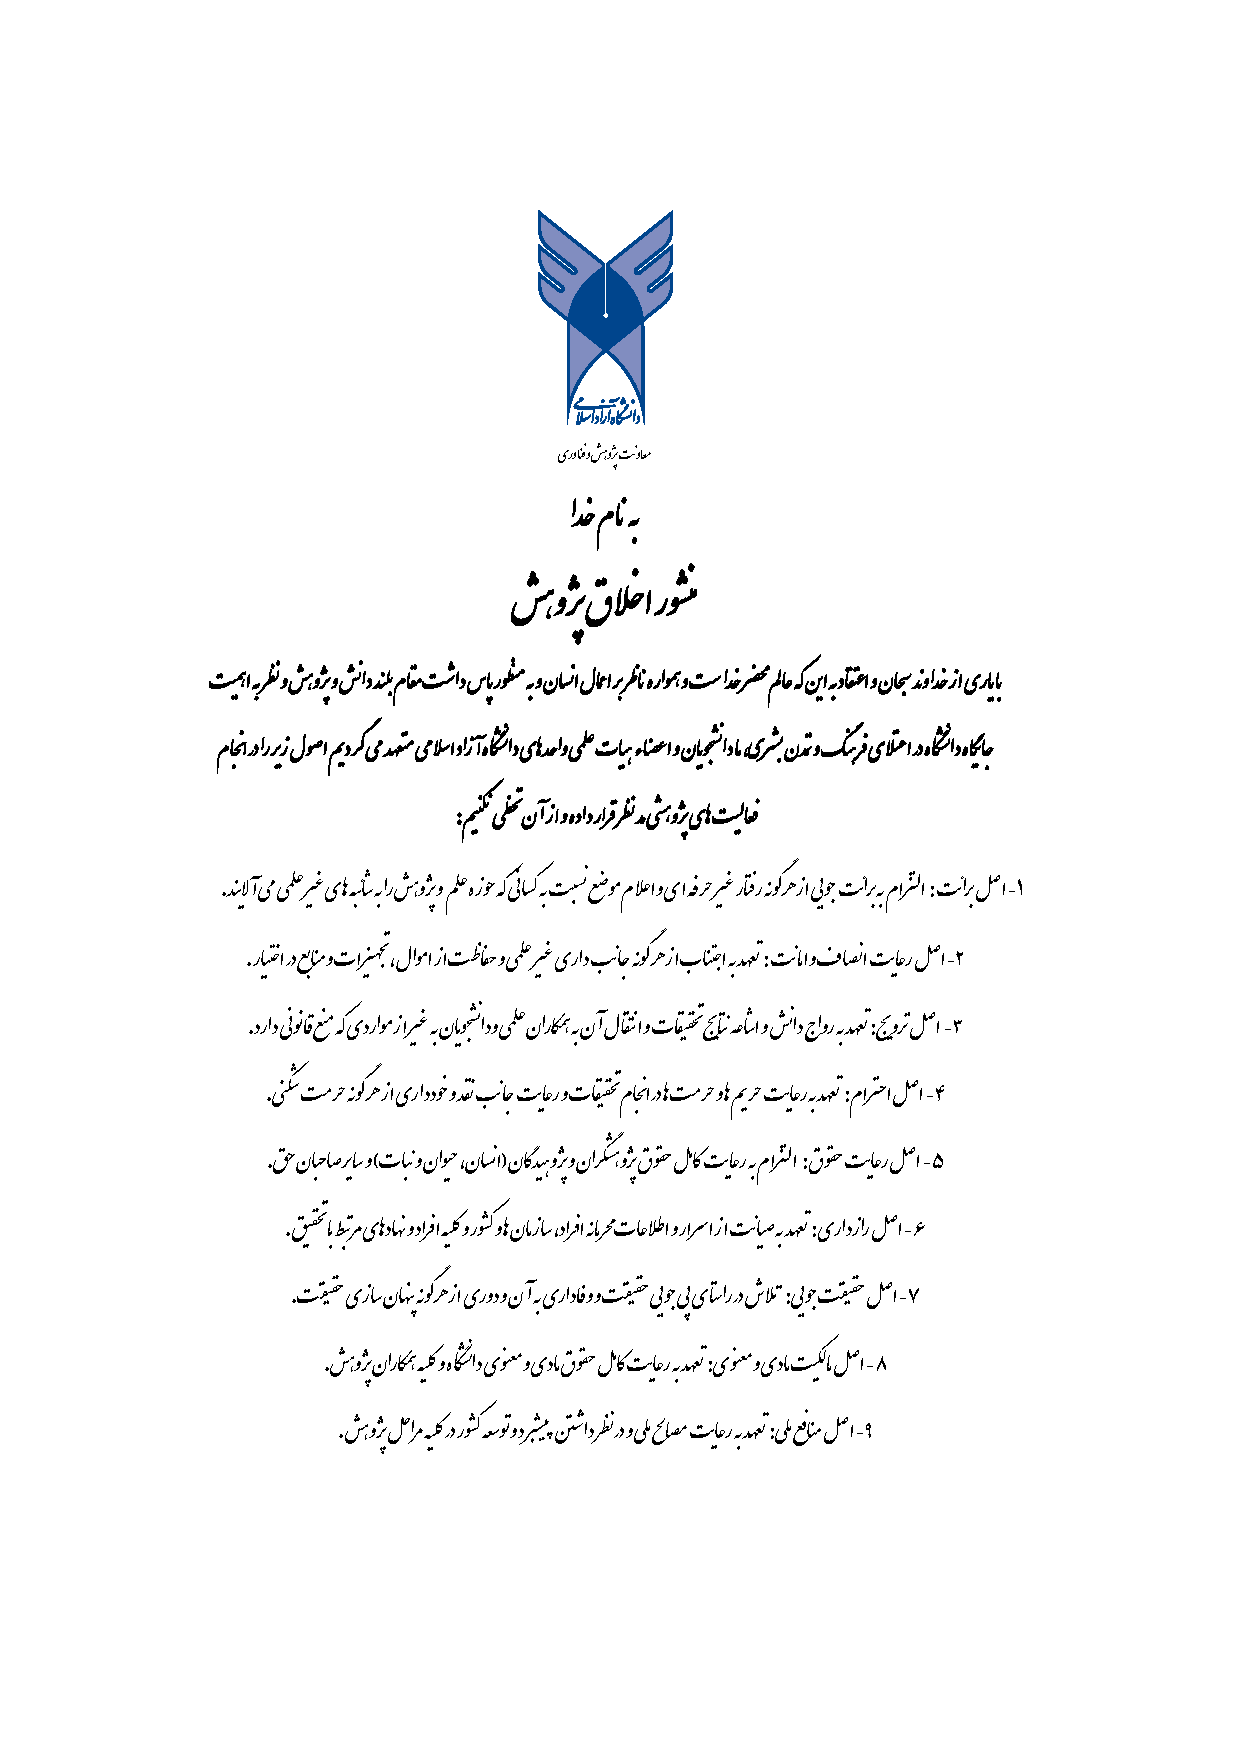
\includepdf[pages=-]{misc/Manshor.pdf}

\thispagestyle{empty}

\noindent
\textbf{\Large تقدیم به:}
\vskip 1cm

\newpage
\thispagestyle{empty}

\begin{center}
\textbf{\Large سپاسگزاری}
\end{center}
\vskip 1cm
\noindent ابتدا از استاد راهنمای خود، جناب آقای دکتر جلال‌الدین نصیری، بسیار سپاسگزارم. ایشان با راهنمایی و توصیه‌های ارزنده‌شان، بنده را در انجام این پژوهش بسیار یاری کردند. همچنین از سرکار خانم دکتر فتاحی  جهت مشاوره و راهنمایی در زمینه‌ی داده‌کاوی و روش تحقیق متشکر هستم. در آخر لازم به ذکر است که پیاده‌سازی و ارزیابی الگوریتم‌ها در آزمایشگاه متن‌کاوی و یادگیری ماشین  پژوهشگاه ایرانداک صورت گرفته است. لذا از ریاست محترم پژوهشگاه ایرانداک برای فراهم کردن امکانات مورد نیاز پژوهش تشکر می‌نمایم. 

\vskip 1cm


\pagenumbering{alph}

% Lists
\tableofcontents
\listoftables
\listoffigures
\listofalgorithms

% Lists customization
\addtocontents{toc}{\textbf{عنوان}~\hfill\textbf{صفحه}\par}
\addtocontents{lot}{\textbf{عنوان}~\hfill\textbf{صفحه}\par}
\addtocontents{lof}{\textbf{عنوان}~\hfill\textbf{صفحه}\par}
\addtocontents{loa}{\textbf{عنوان}~\hfill\textbf{صفحه}\par}

% Notations
% Notatation are summarized

\chapter*{فهرست علائم و نمادها}\markboth{فهرست علائم و نمادها}{فهرست علائم و نمادها}

\baselineskip=0.8cm
\notation{تعداد نمونه‌های آموزشی}{$m$}
\notation{تعداد ویژگی‌ها}{$n$}
\notation{نمونه $i$ام}{$x_i$}

% Reset line space for main content
\baselineskip=0.9cm

% Persian Abstarct

\thispagestyle{plain}
\pagenumbering{arabic}

% Adding abstract to TOC
\addcontentsline{toc}{section}{چکیده}

\noindent
\textbf{\Large چکیده}
\vskip 1 cm
\noindent در دهه اخیر، یادگیری ماشین برای حل کردن مسائل با الگوهای پیچیده استفاده شده است. دسته‌بندی یکی از روش‌های اصلی یادگیری است که مسائلی نظیر تشخیص چهره، تشخیص متون و تشخیص بیماری‌ها را حل می‌کند. ماشین بردار پشتیبان یکی از روش‌های شناخته شده  دسته‌بندی است که دقت و تعمیم پذیری خوبی دارد.

\vskip 3cm
\noindent
\textbf{واژه‌های کلیدی:}


% Chapters
\chapter{کلیات}
\section{مقدمه}

ماشین بردار پشتیبان\footnote{\lr{Support Vector Machine (SVM)}} توسط \lr{Vapnik} در سال 1995 ارائه شد \cite{vapnik1995}.

\lr{\textbf{Support Vector Machine}}
\lr{Support Vector Machine}

\newpage


% Chapter 2 Support Vector Machine

\chapter{پشینیه پژوهش} \label{ch:2}
\section{ماشین بردار پشتیبان} \label{sec:2:1}
در این بخش، ابتدا ماشین بردار پشتیبان خطی و غیر خطی شرح داده می‌شود. سپس پیشینه پژوهش در زمینه ماشین بردار پشتیبان بررسی می‌گردد.
\subsection{ماشین بردار پشتیبان با حاشیه سخت} \label{sec:2:1:1}
ماشین بردار پشتیبان با هدف جداسازی نمونه‌های دو کلاس در سال 1995 معرفی گردید \cite{vapnik1995}. ایده اصلی این روش یادگیری، بدست آوردن ابرصفحه بهینه‌ای است که از نمونه‌های دو کلاس تا جای ممکن بیشترین فاصله را داشته باشد. به عبارت دیگر، این روش یادگیری حاشیه دو کلاس را بیشینه می‌کند. برای فهم بهتر ایده این روش، فرض کنید مجموعه داده‌ی $T=\{(x_1, y_1),(x_2, y_2) \cdots , (x_m, y_m)\}$ را در اختیار داریم که شامل $m$ تا نمونه آموزشی است. هر نمونه آموزشی $x_{i} \in \mathbb{R}^{n}$ با $n$ ویژگی در فضای ورودی و $y_i \in \{-1,1\}$ برچسب نمونه‌ی $x_i$ می‌باشد. در ساده‌ترین حالت، نمونه‌های دو کلاس در مجموعه داده $T$ با یک ابرصفحه $w^{T}x+b$ بدون خطا دسته‌بندی می‌شود. این حالت مسئله حاشیه سخت\footnote{\lr{Hard margin}}  نامیده می‌شود. شکل \ref{fig:SVM-HM} مسئله حاشیه سخت در روش \lr{SVM} را نشان می‌دهد. (لازم به ذکر است، خطوط نقطه‌چین در شکل ‏\ref{fig:SVM-HM} نشان دهنده حاشیه است.) در این حالت، یک مسئله بهینه‌سازی برای بدست آوردن ابرصفحه باید حل گردد.

\begin{equation}
\begin{gathered} 
\mathop{min}\limits_{w}\frac{1}{2}{{\left\| w \right\|}^{2}} \\
\textrm{\lr{s.t. }} {{y}_{i}}({{w}^T}{{x}_{i}}+b)\ge 1,\forall i
\end{gathered}
\label{eq:1}
\end{equation}

\begin{figure}[!t]
	\centering
	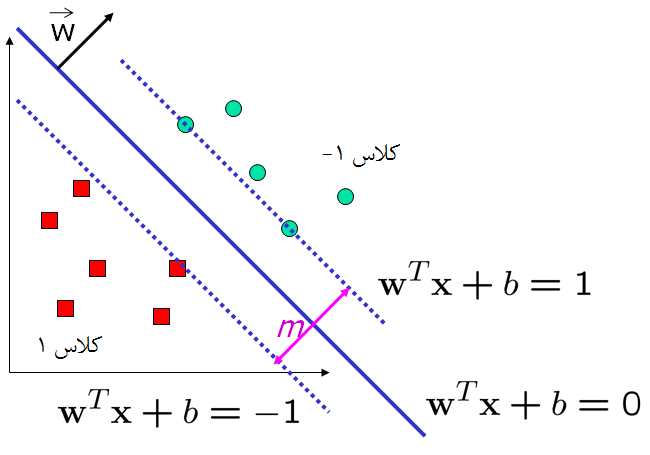
\includegraphics[scale=0.5]{SVM-HardMargin}
	\caption{مسئله حاشیه سخت در ماشین بردار پشتیبان}
	\label{fig:SVM-HM}
\end{figure}

\noindent در رابطه \ref{eq:1}، بردار $w$ مختصات ابرصفحه و $b$ بایاس است. قید این مسئله بهنیه‌سازی بیان می‌کند که تمام نمونه‌های آموزشی باید از ابرصفحه به مقدار 1 یا بیشتر فاصله داشته باشند. به عبارت دیگر، تمام نمونه‌های آموزشی باید روی خط حاشیه یا قبل از آن قرار بگیرند. برای حل کردن مسئله بهینه‌سازی \ref{eq:1} از تابع لاگرانژ\footnote{\lr{Lagrange}}  استفاده می‌شود که در رابطه زیر تعریف شده است. 
\begin{equation}
L(w,b,\alpha )=\frac{1}{2}{{\left\| w \right\|}^{2}}-\sum\limits_{i=1}^{m}{{{\alpha }_{i}}({{y}_{i}}({{w}^{T}}{{x}_{i}}+b)-1})
\label{eq:2}
\end{equation} 
در رابطه \ref{eq:2}، بردار $\alpha$ نشان دهنده ضرایب لاگرانژ است. برای حل کردن رابطه \ref{eq:2}، از تابع لاگرانژ نسبت به $w$ و  $b$ مشتق می‌گیریم.
\begin{align}
\label{eq:3}
\begin{split}
\frac{\partial L}{\partial b}=0&\quad \Rightarrow \quad \sum\limits_{i=1}^{m}{{{\alpha }_{i}}{{y}_{i}}}=0 
\end{split}\\ 
\label{eq:4}
\begin{split}
\frac{\partial L}{\partial w}=0& \quad \Rightarrow \quad w = \sum\limits_{i=1}^{m}{\alpha_{i}y_{i}x_{i}}. 
\end{split} 
\end{align}

با استفاده از اصل دوگانگی لاگرانژ، مسئله اصلی\footnote{\lr{Primal problem}}  در رابطه \ref{eq:1} می‌تواند به مسئله دوگان\footnote{\lr{Dual problem}}  تبدیل شود که حل کردن آن آسان‌تر از مسئله اصلی خواهد بود. با در نظر گرفتن روابط \ref{eq:3} و \ref{eq:4}، مسئله دوگان برای حالت حاشیه سخت به صورت زیر تعریف می‌شود.
\begin{equation}
\begin{split} 
\min\limits_{\alpha} \quad &\frac{1}{2}\sum\limits_{i=1}^{m}{\sum\limits_{j=1}^{m}{{{\alpha }_{i}}{{\alpha }_{j}}{{y}_{i}}{{y}_{j}}x_{i}^{T}{{x}_{j}}-\sum\limits_{k=1}^{m}{{{\alpha }_{k}}}}} \\
\textrm{\lr{s.t. }} \quad &\sum\limits_{i=1}^{m}{\alpha_{i}y_{i}}=0, \\
&\alpha_{i}\ge 0,\text{ }\forall i
\end{split}
\label{eq:5}
\end{equation}
بعد از حل کردن مسئله دوگان \ref{eq:5}، اکثر مقادیر بردار $\alpha$ برابر با صفر خواهد. با این حال ضرایب لاگرانژ  $\alpha_i$ متناظر با نمونه‌های $x_i$ بزرگتر از صفر خواهد بود، اگر معادله زیر برقرار باشد.
\begin{equation}
{{y}_{i}}({{w}^{T}}{{x}_{i}}+b)=1
\label{eq:6}
\end{equation}
\indent نمونه‌های  که رابطه \ref{eq:6} برای آن‌ها برقرار باشد، به اصطلاح بردار پشتیبان\footnote{\lr{Suppor Vector (SV)}}  نامیده می‌شود. ضرایب لاگرانژ متناظر با بردار‌های پشتیبان بزرگ‌تر از صفر است. همچنین این بردارها روی حاشیه قرار می‌گیرند. بردار $w$  و بایاس  $b$ از طریق رابطه  بدست می‌آید.
\begin{equation}
\begin{split}
w &= \sum\limits_{i=1}^{m}{\alpha_{i}y_{i}x_{i}} \\
b &= y_{i}-{w}^{T}{x}_{i}
\end{split}
\label{eq:7}
\end{equation}
یک نمونه جدید یا تست بر اساس تابع تصمیم در رابطه زیر به یکی از کلاس‌های 1 و 1- تعلق می‌گیرد.
\begin{equation}
D(x)=sign({{w}^{T}}x+b) = sign(\sum\limits_{i=1}^{m}{\alpha_{i}y_{i}x_{i}^{T}} x + b)
\label{eq:8}
\end{equation}
\indent در مسئله حاشیه سخت، فرض گرفته می‌شود که تمام نمونه‌های دو کلاس به صورت خطی جدا پذیر هستند. با این حال در دنیای واقعی داده‌ها اغلب به صورت خطی جدا پذیر نیستند. در حالتی که داده‌ها به صورتی خطی جداپذیر نیستند، مسئله حاشیه نرم\footnote{\lr{Soft margin}}  در ماشین بردار پشتیبان مطرح شده است.

\subsection{ماشین بردار پشتیبان با حاشیه نرم} \label{sec:2:1:2}
در این حالت اجازه خطا در دسته‌بندی نمونه‌ها داده می‌شود. به عبارت دیگر، با معرفی متغیر کمکی\footnote{\lr{Slack variable}} $\xi$ ، تاثیر بعضی از نمونه‌های آموزشی در ایجاد حاشیه و ابرصفحه کم می‌شود. برای درک بهتر، مسئله حاشیه نرم در ماشین بردار پشتیبان در شکل \ref{fig:SVM-SM}‏ نشان داده شده است. در حالت حاشیه نرم، برای بدست آوردن ابرصفحه مسئله بهینه‌سازی به صورت زیر تعریف می‌شود.

\begin{figure}[!t]
	\centering
	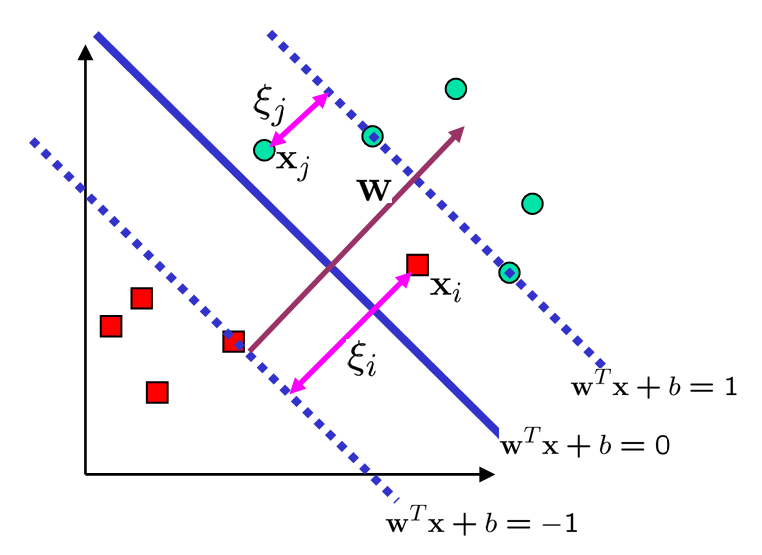
\includegraphics[scale=0.5]{SVM-SoftMargin}
	\caption{مسئله حاشیه نرم در ماشین بردار پشتیبان}
	\label{fig:SVM-SM}
\end{figure}

\begin{equation}
\begin{split}
\min_{w} \quad &\frac{1}{2}{{\left\| w \right\|}^{2}}+C\sum\limits_{i=1}^{n}{{{\xi }_{i}}} \\
\textrm{\lr{s.t. }}  \quad &{{y}_{i}}({{w}^{T}}{{x}_{i}}+b)\text{ }+{{\xi }_{i}}\ge 1,\forall i
\end{split}
\label{eq:9}
\end{equation}
در رابطه \ref{eq:9}، متغیر $\xi _{i}\ge 0$ خطای متناظر برای هر نمونه  $x_i$ است. پارامتر $C$ بیانگر تعادل بین بیشینه کردن حاشیه و خطای دسته‌بندی است. مقدار این پارامتر قبل از آموزش دسته‌بند باید مشخص گردد. مانند مسئله حاشیه سخت، برای حل کردن مسئله اصلی  از تابع لاگرانژ استفاده می‌شود که در رابطه زیر تعریف شده است.
\begin{equation}
L(w,b,\xi, \alpha, \beta )=\frac{1}{2}{{\left\| w \right\|}^{2}} + C\sum\limits_{i=1}^{m}{{{\xi }_{i}}}  -\sum\limits_{i=1}^{m}{{{\alpha }_{i}}({{y}_{i}}({{w}^{T}}{{x}_{i}}+b)-1 + \xi_{i} }) - \sum\limits_{i=1}^{m}{\beta_{i}\xi_{i}}
\label{eq:10}
\end{equation}
در رابطه \ref{eq:10}، بردار $\alpha$  و $\beta$  ضرایب لاگرانژ هستند. برای حل کردن رابطه \ref{eq:10}، نسبت به  $w$، $b$ و $\xi$  مشتق می‌گیریم.
\begin{align}
\label{eq:11}
\begin{split}
\frac{\partial L}{\partial b}&=0\quad \Rightarrow \quad \sum\limits_{i=1}^{m}{{{\alpha }_{i}}{{y}_{i}}}=0
\end{split}\\ 
\label{eq:12}
\begin{split}
\frac{\partial L}{\partial w}&=0 \quad \Rightarrow \quad w = \sum\limits_{i=1}^{m}{\alpha_{i}y_{i}x_{i}}.
\end{split}\\
\label{eq:13}
\begin{split}
\frac{\partial L}{\partial \xi}&=0 \quad \Rightarrow \quad \alpha_{i} + \beta_{i} = C
\end{split}  
\end{align}
با در نظر گرفتن روابط بالا، مسئله دوگان برای حالت حاشیه نرم به صورت زیر تعریف می‌شود.
\begin{equation}
\begin{split} 
\min\limits_{\alpha} \quad &\frac{1}{2}\sum\limits_{i=1}^{m}{\sum\limits_{j=1}^{m}{{{\alpha }_{i}}{{\alpha }_{j}}{{y}_{i}}{{y}_{j}}x_{i}^{T}{{x}_{j}}-\sum\limits_{k=1}^{m}{{{\alpha }_{k}}}}} \\
\textrm{\lr{s.t. }} \quad &\sum\limits_{i=1}^{m}{\alpha_{i}y_{i}}=0, \\
&0 \le \alpha_{i}\le C,\text{ }\forall i
\end{split}
\label{eq:14}
\end{equation}
\indent راه حل مسئله \ref{eq:14} شبیه به مسئله \ref{eq:5} در حالت حاشیه سخت است. با این تفاوت که برای ضرایب لاگرانژ یک حد بین صفر تا پارامتر  تعریف شده است. پارامتر  انعطاف‌پذیری دسته‌بند را افزایش می‌دهد. مقدار این پارامتر با داشتن دانش قبلی از مسئله و یا جستجوی شبکه‌ای تعیین می‌شود. همانطور که در شکل ‏\ref{fig:SVM-SM} نشان داده شده است، بردارهای پشتیبان لزوما روی خط حاشیه قرار ندارند. در مسئله حاشیه نرم، تابع تصمیم مشابه حالت حاشیه سخت به صورت زیر تعریف می‌شود.
\begin{equation}
D(x)=sign({{w}^{T}}x+b) = sign(\sum\limits_{i \in S}{\alpha_{i}y_{i}x_{i}^{T}} x + b)
\label{eq:15}
\end{equation}
در رابطه \ref{eq:15}، مجموعه $S$ نشان دهنده بردارهای پشتیبان است.

\subsection{ماشین بردار پشتیبان با هسته غیر خطی}\label{sec:2:1:3}
در مسائل حاشیه سخت و نرم، فرض گرفته می‌شود که نمونه‌ها در فضای ورودی به صورت خطی جدا پذیر هستند. با این حال در مواردی که نمونه‌ها به صورت خطی جدا پذیر نیستند، نمونه‌ها $x_i$ به فضای ویژگی\footnote{\lr{Feature space}}  با ابعاد بیشتر با تکنیک حقه‌ی هسته\footnote{\lr{Kernel trick}}  نگاشت می‌شود. در این فضا، ماشین بردار پشتیبان یک ابرصفحه جدا کننده بهینه برای جداسازی نمونه‌ها پیدا می‌کند. شکل \ref{fig:SVM-Ker} تکنیک حقه‌ی هسته را نشان می‌دهد.

\begin{figure}[!t]
	\centering
	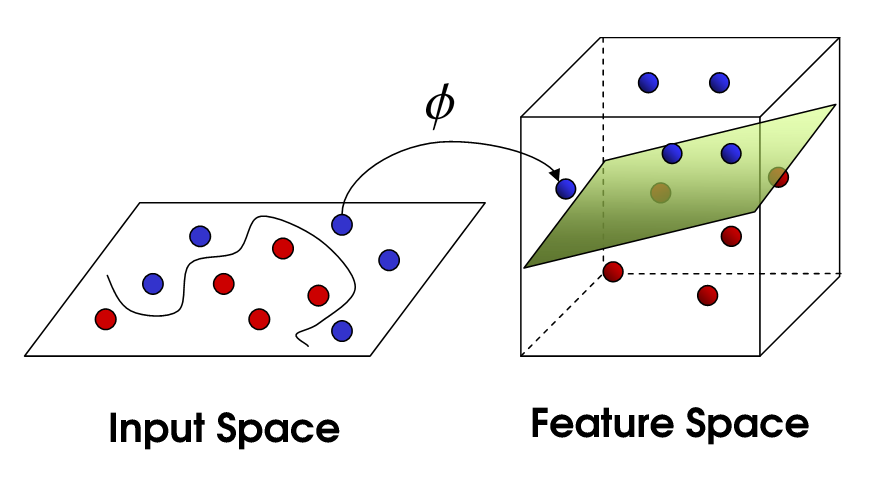
\includegraphics[scale=0.4]{SVM-Kernel}
	\caption{نگاشت نمونه‌ها با تکنیک حقه‌ی هسته}
	\label{fig:SVM-Ker}
\end{figure}

در نسخه غیر خطی ماشین بردار پشتیبان، مسئله \ref{eq:14} به صورت زیر تعریف می‌شود.
\begin{equation}
\begin{split} 
\min\limits_{\alpha} \quad &\frac{1}{2}\sum\limits_{i=1}^{m}{\sum\limits_{j=1}^{m}{{{\alpha }_{i}}{{\alpha }_{j}}{{y}_{i}}{{y}_{j}}K(x_{i},{{x}_{j}})-\sum\limits_{k=1}^{m}{{{\alpha }_{k}}}}} \\
\textrm{\lr{s.t. }} \quad &\sum\limits_{i=1}^{m}{\alpha_{i}y_{i}}=0, \\
&0 \le \alpha_{i}\le C,\text{ }\forall i
\end{split}
\label{eq:16}
\end{equation}
در رابطه \ref{eq:16}‏، تابع هسته  $K({{x}_{i}},{{x}_{j}})$ نمونه‌ها را به فضای ویژگی نگاشت می‌کند. تابع‌های هسته متداول شامل  \lr{RBF}\footnote{\lr{Radial basis function (RBF)}}، چند جمله‌ای و سیگموئید\footnote{\lr{Sigmoid}}  هستند. تابع تصمیم در نسخه غیر خطی به صورت زیر تعریف می‌شود.
\begin{equation}
D(x)= sign(\sum\limits_{i \in S}{\alpha_{i}y_{i}}K(x_{i}, x) + b)
\label{eq:17}
\end{equation}

\subsection{ماشین بردار پشتیبان چندکلاسه}\label{sec:2:1:5}
ماشین بردار پشتیبان برای دسته‌بندی دو کلاس ارائه شده است. به منظور تعمیم ماشین بردار پشتیبان به مسائل چند کلاسه، به طور کلی دو روش وجود دارد \cite{hsu2002}:
\begin{enumerate}
	\item  ایجاد و ترکیب چندین دسته‌بند دوکلاسه برای حل کردن مسائل چند کلاسه
	\item لحاظ کردن تمام نمونه‌های آموزشی در یک مسئله بهینه‌سازی بزرگ
\end{enumerate}

روش اول برای حل مسائل چند کلاسه بیشتر مورد توجه گرفته است. بطوریکه سه نوع روش ایجاد و ترکیب چندین دسته‌بند شامل یک-در مقابل-بقیه\footnote{\lr{One-Against-All}}، یک-در مقابل-یک\footnote{\lr{One-Against-One}} و گراف جهت‌دار یک-در مقابل-یک ارائه شده است \cite{hsu2002, shigeo2005}. در ادامه هر یک از این روش‌های چند کلاسه توضیح داده می‌شود.
\subsubsection{یک-در مقابل-بقیه}\label{sec:2:1:5:1}
 روش یک-در مقابل-بقیه قدیمی‌ترین روش چندکلاسه برای دسته‌بند \lr{SVM} است. برای تشریح این روش چند کلاسه، ابتدا یک مسئله دسته‌بندی $k$کلاسه با مجموعه داده $T=\{(x_1, y_1),(x_2, y_2) \cdots , (x_m, y_m)\}$ را در نظر می‌گیریم. $x_{i} \in \mathbb{R}^{n}$  نشان‌دهنده نمونه آموزشی و $y_i \in \{1,\dots, k\}$ کلاس نمونه $x_{i}$ را نشان می‌دهد. $k$دسته‌بند \lr{SVM} دو دسته‌ای در روش یک-در مقابل-بقیه آموزش داده می‌شود. بطوریکه $k$ برابر با تعداد کلاس‌ها است. در اینجا $i$مین تابع تصمیم $D_{i}(x) = w^{T}_{i}\varphi(x) + b_{i}$ کلاس $i$ام را از سایر کلاس‌ها جدا می‌کند.
 
به منظور پیدا کردن کلاس داده تست، ابتدا مقادیر تابع تصمیم $D_{i}(x)$ برای $k$دسته‌بند محاسبه می‌شود. چنانچه به ازای فقط یک  $i$ مقدار $D_{i}(x) > 0$ برقرار باشد، آنگاه داده تست به کلاس $i$ام تعلق دارد. با این حال امکان دارد که برای یک داده تست چندین مقدار $D_{i}$ مثبت یا مقادیر تمامی توابع تصمیم منفی شوند. در این حالت، امکان دسته‌بندی داده تست وجود ندارد. این مشکل تحت عنوان نواحی غیر قابل دسته‌بندی\footnote{\lr{Unclassifiable region}} شناخته می‌شود. شکل \ref{fig:SVM-OVA} نواحی غیر قابل دسته‌بندی در روش یک-در مقابل-بقیه را نشان می‌دهد. این نواحی در شکل با هاشور مشخص شده‌اند.

\begin{figure}[!t]
	\centering
	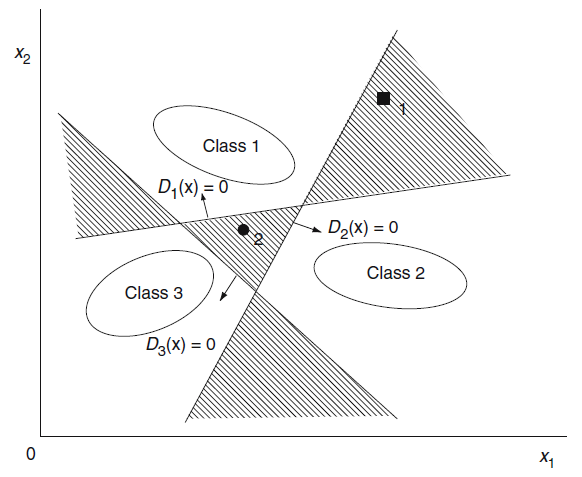
\includegraphics[scale=0.4]{SVM-OVA}
	\caption[نواحی غیر قابل دسته‌بندی در روش یک-در مقابل-بقیه]{نواحی غیر قابل دسته‌بندی در روش یک-در مقابل-بقیه \cite{shigeo2005}}
	\label{fig:SVM-OVA}
\end{figure}

برای مثال، نمونه ۱ در شکل \ref{fig:SVM-OVA} در ناحیه تصمیم دو کلاس ۱ و ۲ قرار دارد. بطوریکه مقدار $D_{1}(x_{1}) > 0$  و $D_{2}(x_{1}) > 0$ برقرار است. بنابراین کلاس نمونه ۱ غیر قابل تشخیص است.  

\subsubsection{یک-در مقابل-یک}\label{sec:2:1:5:2}
این روش برای یک مسئله دسته‌بندی با $k$ کلاس، $k(k-1)/2$ دسته‌بند دودسته‌ای ایجاد می‌کند \cite{hsu2002}. در اینجا هر دسته‌بند فقط با نمونه‌های دو کلاس آموزش داده می‌شود. تابع تصمیم $D_{ij}(x) = w^{T}_{ij}\varphi(x) + b_{ij}$  در روش یک-در مقابل-یک کلاس $i$ام را از کلاس $j$ام جدا می‌کند.

به منظور تعیین کلاس داده تست در روش یک-در مقابل-یک، از رای‌گیری\footnote{\lr{Voting}} استفاده می‌شود. چنانچه $sign(w^{T}_{ij}\varphi(x) + b_{ij})$ مشخص کند که نمونه تست $x$ به کلاس $i$ام تعلق دارد، آنگاه رای برای کلاس $i$ام یکی افزایش پیدا می‌کند. در غیر این صورت، رای کلاس $j$ام یکی افزایش می‌یابد. در آخر نمونه تست $x$ به کلاسی با بیشترین رای تعلق می‌گیرد. شکل \ref{fig:SVM-OVO} نواحی غیر قابل دسته‌بندی در روش یک-در مقابل-یک را نشان می‌دهد.

\begin{figure}[!t]
	\centering
	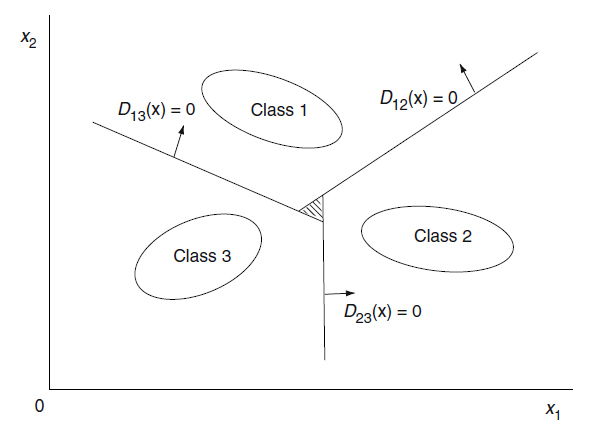
\includegraphics[scale=0.4]{SVM-OVO}
	\caption[نواحی غیر قابل دسته‌بندی در روش یک-در مقابل-یک]{نواحی غیر قابل دسته‌بندی در روش یک-در مقابل-یک \cite{shigeo2005}}
	\label{fig:SVM-OVO}
\end{figure}

همانطور که در شکل \ref{fig:SVM-OVO} مشخص است، نواحی غیر قابل دسته‌بندی در روش یک-در مقابل-یک بسیار کوچکتر از روش یک-در مقابل-بقیه است. روش یک-در مقابل-یک با وجود داشتن دقت دسته‌بندی بهتر، پیچیدگی محاسباتی زیادی دارد. برای مثال‌، یک مسئله با ۱۰ کلاس نیاز به آموزش دادن ۴۵ دسته‌بند دودسته‌ای دارد. 

\subsubsection{گراف جهت‌دار یک-در مقابل-یک}\label{sec:2:1:6}
به منظور برطرف کردن نواحی غیر قابل دسته‌بندی در روش یک-در مقابل-یک، گراف تصمیم جهت‌دار غیرچرخه‌ای\footnote{\lr{Directed Acyclic Graph (DAG)}} ارائه شده است \cite{platt2000}. فرآیند آموزش این روش همانند روش یک-در مقابل-یک است و $k(k-1)/2$ دسته‌بند دودسته‌ای را ایجاد می‌کند. با این حال بدست آوردن کلاس نمونه تست با استفاده از یک گراف دودویی \lr{DAG} با $k(k-1)/2$ گره میانی و $k$ برگ انجام می‌شود. در واقع هر گره در این گراف،  یک دسته‌بند دودسته‌ای برای کلاس $i$ و $j$ است. شکل \ref{fig:SVM-DAG} گراف دودویی \lr{DAG} برای سه کلاس نشان می‌دهد.

\begin{figure}[!t]
	\centering
	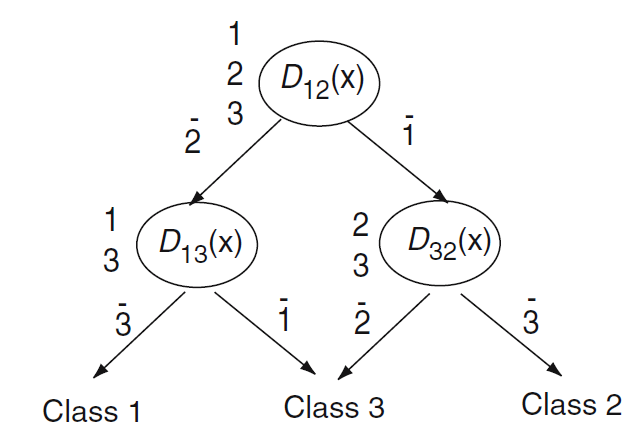
\includegraphics[scale=0.4]{SVM-DAG}
	\caption[گراف دودویی \lr{DAG} برای سه کلاس]{گراف دودویی \lr{DAG} برای سه کلاس \cite{shigeo2005}}
	\label{fig:SVM-DAG}
\end{figure}

پیدا کردن کلاس داده تست از گره ریشه آغاز می‌شود و سپس با توجه به خروجی تابع تصمیم حرکت به سمت چپ یا راست گراف صورت می‌گیرد. حرکت  تا رسیدن به گره برگ ادامه می‌یابد. گره برگ نشان‌دهنده کلاس داده تست است. دیگر مزیت روش \lr{DAG} نسبت به روش یک-در مقابل-یک کمتر بودن زمان تست می‌باشد.


\subsection{پیشینه پژوهش در ماشین بردار پشتیبان}\label{sec:2:1:4}
ماشین بردار پشتیبان بنیان ریاضی قوی‌ای دارد و دارای قدرت تعمیم‌پذیری بالایی است. از این رو در مسائل مختلف انند تشخیص آریتمی‌های قلبی \cite{nasiri2009}، شناسایی نفوذ به شبکه‌های کامپیوتری \cite{raman2017}، دسته‌بندی متن\cite{lee2012} و شناسایی 
هرزنامه \cite{zoubi2018} مورد استفاده قرار گرفته است. با این حال ماشین بردار پشتیبان نقاط ضعفی نیز دارد که مهم‌ترین آن‌ها عبارتند از:
\begin{enumerate}
	\item ماشین بردار پشتیبان برای بدست آوردن ابرصفحه بهینه یک مسئله بهینه‌سازی از نوع برنامه‌ریزی درجه دو حل می‌کند. مرتبه زمانی حل کردن چنین مسئله‌ای برابر با   $\mathcal{O}({{m}^{3}})$ است.  $m$ تعداد نمونه‌های آموزشی می‌باشد. این مرتبه زمانی، آموزش روش ماشین بردار پشتیبان را برای مجموعه داده‌های بزرگ به طور قابل توجه‌ای کند می‌کند.
	\item در روش \lr{SVM}، بردارهای پشتیبان نقش مهمی در ایجاد مدل دارند. در صورتی که این بردارها از نمونه‌های پرت یا نویزی باشد، دقت و تعمیم‌پذیری مدل خروجی کاهش می‌یابد. در نتیجه روش \lr{SVM} به نمونه‌های پرت و نویزی حساس است.
	\item چنانچه نمونه‌های یک کلاس از کلاس دیگر بسیار بیشتر باشد (مجموعه داده نامتوازن باشد.)، مدل ایجاد شده توسط  \lr{SVM} به سمت کلاس اکثریت گرایش پیدا می‌کند. در نتیجه مدل در تشخیص کلاس اقلیت ناتوان است.
\end{enumerate}

\indent در دو دهه اخیر، روش‌های یادگیری جدیدی مبتنی \lr{SVM} ارائه شده است که برخی از آن‌ها نقاط ضعف بالا را حل می‌کند. در سال 1999، ماشین بردار پشتیبان کمترین مربعات\footnote{\lr{Least squares support vector machines  (LS-SVM)}}  ارائه شد \cite{suykens1999}. در این روش قید در مسئله بهینه‌سازی از نامساوی به مساوی تبدیل شده است. بطوریکه به جای حل کردن مسئله بهینه‌سازی از نوع برنامه‌ریزی درجه دو، دستگاه معادلات خطی حل می‌گردد. در نتیجه سرعت یادگیری برای مجموعه داده‌های بزرگ بسیار بیشتر می‌شود و نقطه ضعف مورد اول تا حد زیادی حل شده است.

در سال 2001، ماشین بردار پشتیبان مبتنی بر مفهوم نزدیکی\footnote{\lr{Proximal Support Vector Machine (PSVM)}}  (\lr{PSVM}) ارائه شد \cite{mang2001}. در این روش دو ابرصفحه موازی برای دسته‌بندی نمونه‌ها ایجاد می‌شود. در سال 2002، ماشین بردار پشتیبان فازی\footnote{\lr{Fuzzy Support Vector Machine (FSVM)}}  (\lr{FSVM}) \cite{lin2002} ارائه گردید. در این روش به هر یک از نمونه‌های هر دو کلاس، تعلق فازی داده می‌شود. بطوریکه اثر نمونه‌های نویزی و پرت در ایجاد مدل خروجی کم خواهد شد. در سال 2006، ماشین بردار پشتیبان با رویکرد مقدار ویژه تعمیم یافته\footnote{\lr{Generalized Eigenvalue Proximal Support Vector Machine (GEPSVM)}}  (\lr{GEPSVM}) ارائه شد \cite{mang2006}. برخلاف روش \lr{PSVM}، این روش دو ابرصفحه غیر موازی ایجاد می‌کند که هر یک از این ابرصفحه‌ها به نمونه‌های کلاس خود نزدیک است و از نمونه‌های کلاس مقابل تا جای ممکن فاصله می‌گیرد. همچنین روش \lr{PSVM} بر روی مسئله \lr{XOR} عملکرد بهتری نسبت به روش \lr{SVM} اصلی دارد.

در سال 2007، ماشین بردار پشتیبان دو قلو\footnote{\lr{Twin Support Vector Machine (TSVM)}}  (\lr{TSVM}) با هدف بهبود پیچیدگی زمانی \lr{SVM} ارائه گردید \cite{jayadeva2007}. ایده اصلی این روش یادگیری، بدست آوردن دو ابرصفحه غیر موازی است. بطوریکه هر ابرصفحه غیر موازی به نمونه‌های کلاس خود نزدیک است و نمونه‌های کلاس مقابل دور می‌شود. دو مسئله بهینه‌سازی کوچک از نوع برنامه‌ریزی درجه دو برای بدست آوردن این دو ابرصفحه غیر موازی حل می‌گردد. در حالی‌که در روش \lr{SVM} یک مسئله بهینه‌سازی بزرگ حل می‌شود. در نتیجه، روش ماشین بردار پشتیبان دو قلو در تئوری 4 برابر سریعتر از روش \lr{SVM} است. در بخش ‏2-2 ماشین بردار پشتیبان دو قلو و پیشینه پژوهش آن به طور کامل بررسی می‌شود.

در سال‌های اخیر نیز، روش‌های جدید مبتنی بر \lr{SVM} ارائه شده است. در سال 2018، می‌توان به روش یادگیری برخط مبتنی بر بدترین نمونه‌ی نقض‌کننده\footnote{\lr{Online Learning Algorithm using Worst-Violators (OLLAWV)}}  اشاره کرد \cite{melki2018}. این الگوریتم بر اساس گرادیان نزولی تصادفی\footnote{\lr{Stochastic Gradient Descent (SGD)}}  طراحی شده است و مسئله اصلی در روش \lr{SVM} را به جای مسئله دوگان حل می‌کند. مزایای این روش، دقت بهتر، سرعت یادگیری بیشتر برای مجموعه داده‌های بزرگ و همچنین مدل خلوت\footnote{\lr{Sparse}}  می‌باشد.

\section{ماشین بردار پشتیبان دو قلو}\label{sec:2:2}
در این بخش، ابتدا نسخه خطی ماشین بردار پشتیبان دو قلو شرح داده می شود. سپس نسخه غیر خطی این روش توضیح داده شده و در آخر پیشینه پژوهش آن و روش‌های مبتنی بر \lr{TSVM} بررسی می‌شود.

\subsection{ماشین بردار پشتیبان دو قلو خطی}\label{sec:2:2:1}
ایده اصلی روش \lr{TSVM}، ایجاد دو ابرصفحه غیر موازی است \cite{jayadeva2007}. بطوریکه هر ابرصفحه غیر موازی از نمونه‌های کلاس خود کمترین فاصله را دارد و از نمونه‌های کلاس مقابل حداکثر فاصله ممکن را خواهد داشت. برای تشریح بهتر این روش، یک مسئله دسته‌بندی دوکلاسه با $m_1$  نمونه آموزشی کلاس مثبت و  $m_2$ نمونه آموزشی کلاس منفی را در نظر می‌گیریم. همچنین فرض می‌کنیم که ماتریس   $A\in {{\mathbb{R}}^{{{m}_{1}}\times n}}$ بیانگر نمونه‌های کلاس مثبت و ماتریس  $B\in {{\mathbb{R}}^{{{m}_{2}}\times n}}$ بیانگر نمونه‌های کلاس منفی است. روش \lr{TSVM} در حالت خطی به دنبال دو ابرصفحه غیر موازی در فضای  ${{\mathbb{R}}^{n}}$ است که در رابطه زیر تعریف شده است.
\begin{equation}
{{x}^T}{{w}_{1}}+{{b}_{1}}=0 \quad \textrm{\lr{and }} \quad {{x}^T}{{w}_{2}}+{{b}_{2}}=0
\label{eq:18}
\end{equation}
در رابطه \ref{eq:18}،  ${{w}^{(1)}},{{w}^{(2)}}\in {{\mathbb{R}}^{n}}$ نشان دهنده مختصات دو ابرصفحه و  ${{b}^{(1)}},{{b}^{(2)}}\in {\mathbb{R}}$ نشان دهنده بایاس است. شکل ‏2 4 تفسیر هندسی روش ماشین بردار پشتیبان دوقلو خطی را نشان می‌دهد. در روش \lr{TSVM}، دو مسئله بهینه‌سازی از نوع برنامه‌ریزی درجه دو برای بدست آوردن دو ابرصفحه غیر موازی به صورت زیر تعریف می‌شود.
\begin{figure}[!t]
	\centering
	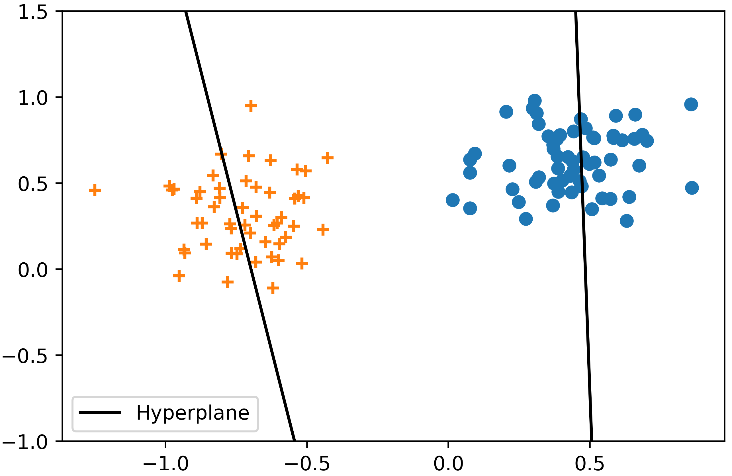
\includegraphics[scale=0.75]{TSVM-idea}
	\caption{تفسیر هندسی روش ماشین بردار پشتیبان دو قلو خطی}
	\label{fig:TSVM-idea}
\end{figure}
\begin{align}
\label{eq:19}
\begin{split}
\underset{{{w}_{(1)}},{{b}_{(1)}}}{\mathop{min}}\,\qquad  & \frac{1}{2}{{\left\| A{{w}^{(1)}}+{{e}_{1}}{{b}^{(1)}} \right\|}^{2}}+{{C}_{1}}e_{2}^{T}{{y}_{2}}  \\
\text{\lr{s.t.}} \qquad  & -(B{{w}^{(1)}}+{{e}_{2}}{{b}^{(1)}})+{{y}_{2}}\ge {{e}_{2}}\text{ },{{y}_{2}}\ge 0  
\end{split} \\
%\end{equation}
%\begin{equation}
\label{eq:20}
\begin{split}
\underset{{{w}_{(2)}},{{b}_{(2)}}}{\mathop{min}}\,\qquad  & \frac{1}{2}{{\left\| B{{w}^{(2)}}+{{e}_{2}}{{b}^{(2)}} \right\|}^{2}}+{{C}_{2}}e_{1}^{T}{{y}_{1}}  \\
\text{\lr{s.t.}} \qquad  & (A{{w}^{(2)}}+{{e}_{1}}{{b}^{(2)}})+{{y}_{1}}\ge {{e}_{1}}\text{ },{{y}_{1}}\ge 0  
\end{split}
\end{align}
\bigbreak
در روابط \ref{eq:19} و \ref{eq:20}،  $C_1$ و $C_2$  پارامترهای خطا،  $e_1$ و  $e_2$ بردار با درایه‌های یک در ابعاد متناسب،  $y_1$ و $y_2$  متغیر کمکی هستند. لازم به ذکر است که تعداد نمونه‌ها در مسائل بهینه‌سازی روش \lr{TSVM} تقریبا برابر با $m/2$ در نظر گرفته می‌شود. با این حال در روش \lr{SVM}، در قید مسئله بهینه‌سازی تمام نمونه‌های آموزشی نقش دارند. بنابراین زمان اجرای روش \lr{TSVM} از روش \lr{SVM} حدود 4 برابر سریع‌تر است که زیر نشان داده شده است.
\begin{equation}
\Big[({{m}^{3}})/(2\times {{(\frac{m}{2})}^{3}})\Big] = 4.
\label{eq:21}
\end{equation}

مانند روش \lr{SVM}، برای حل کردن مسائل بهینه‌سازی \ref{eq:19}، از تابع لاگرانژ استفاده می‌کنیم.
\begin{equation}
\begin{split}
L(w_{1},b_{1},y_{2}, \alpha, \beta )= &\frac{1}{2}(A{{w}^{(1)}}+{{e}_{1}}{{b}^{(1)}})^{T}(A{{w}^{(1)}}+{{e}_{1}}{{b}^{(1)}}) + {{C}_{1}}e_{2}^{T}y_{2} \\
&-\alpha^{T}(-(Bw^{(1)}+e_{2}b^{(1)})+y_{2} - e_{2}) - \beta^{T}y_{2}
\end{split}
\label{eq:22}
\end{equation}

در رابطه \ref{eq:22}، $\alpha=(\alpha_{1}, \alpha_{2}, \dots,\alpha_{m_{2}})^{T}$ و $\beta=(\beta_{1}, \beta_{2}, \dots,\beta_{m_{2}})^{T}$ بردارهای ضرایب لاگرانژ هستند.  با مشتق‌گیری از رابطه \ref{eq:22}، شرایط \lr{KKT}\footnote{\lr{Karush-Kuhn-Tucker}}  زیر برقرار می‌شود.
\begin{align}
\label{eq:23}
\begin{split}
A^{T}(A{{w}^{(1)}}+{{e}_{1}}{{b}^{(1)}}) + B^{T}\alpha = 0.
\end{split} \\
\label{eq:24}
\begin{split}
e_{1}^{T}(A{{w}^{(1)}}+{{e}_{1}}{{b}^{(1)}}) + e_{2}^{T}\alpha = 0.
\end{split}\\
\label{eq:25}
\begin{split}
C_{1}e_{2} - \alpha - \beta = 0.
\end{split} 
\end{align}
با توجه اینکه $\beta \ge 0$، از رابطه \ref{eq:25} خواهیم داشت:
\begin{equation}
0 \le \alpha \le {C}_{1}
\label{eq:26}
\end{equation}

سپس با ترکیب کردن \ref{eq:23} و \ref{eq:24}، رابطه زیر بدست می‌آید.
\begin{equation}
[A^{T}\ e^{T}_{1}][A\ e_{1}][w^{(1)}\ b^{(1)}]^{T} + [B^{T}\ e^{T}_{2}]\alpha = 0.
\label{eq:27}
\end{equation}

با تعریف کردن ماتریس $H$ و $G$ به صورت $H=[A\text{ }e]$ و $G=[B\text{ }e]$، رابطه \ref{eq:27} به صورت زیر بازنویسی می‌شود.
\begin{equation}
\left[ \begin{matrix}
{{w}^{(1)}} \\
{{b}^{(1)}} \\
\end{matrix} \right]= -{{({{H}^{T}}H)}^{-1}}{{G}^{T}}\alpha
\label{eq:28}
\end{equation}

برای جلوگیری از شرایط ماتریس منفرد\footnote{\lr{Singular}}  در ماتریس $H^{T}H$، یک عدد ثابت بسیار کوچک  $\varepsilon > 0, \varepsilon I$ به عناصر قطر این ماتریس اضافه می‌شود. بنابراین دستگاه معادلات در رابطه \ref{eq:28} به صورت زیر تغییر می‌یابد.
\begin{equation}
\left[ \begin{matrix}
{{w}^{(1)}} \\
{{b}^{(1)}} \\
\end{matrix}\right]= -{{({{H}^{T}}H + \varepsilon I)}^{-1}}{{G}^{T}}\alpha
\label{eq:29}
\end{equation}

با توجه به شرایط \lr{KKT} و مسئله اصلی \ref{eq:19}، مسئله دوگان برای \ref{eq:19} به صورت زیر تعریف می‌گردد.
\begin{equation}
\begin{split}
\mathop{{ min}}\limits_{\alpha} \qquad & \frac{1}{2}{{\alpha }^{T}}G{{({{H}^{T}}H)}^{-1}}{{G}^{T}}\alpha -e_{2}^{T}\alpha  \\
\textrm{\lr{s.t. }} \qquad & 0{{e}_{2}}\le \alpha \le {{C}_{1}}{{e}_{2}}
\end{split}
\label{eq:30}
\end{equation}

مشابه راه حل کلاس مثبت، مسئله دوگان برای کلاس منفی \ref{eq:20} به صورت زیر تعریف می‌شود.
\begin{equation}
\begin{split}
\mathop{{ min}}\limits_{\alpha} \qquad & \frac{1}{2}{{\alpha }^{T}}G{{({{H}^{T}}H)}^{-1}}{{G}^{T}}\alpha -e_{2}^{T}\alpha  \\
\textrm{\lr{s.t. }} \qquad & 0{{e}_{2}}\le \alpha \le {{C}_{1}}{{e}_{2}}
\end{split}
\label{eq:31}
\end{equation}

بعد از حل کردن مسئله دوگان \ref{eq:31}، ابرصفحه کلاس منفی از طریق رابطه زیر بدست می‌آید.
\begin{equation}
\left[ \begin{matrix}
{{w}^{(2)}} \\
{{b}^{(2)}} \\
\end{matrix}\right]= {{({{G}^{T}}G)}^{-1}}{{H}^{T}}\beta
\label{eq:32}
\end{equation}

در نسخه خطی روش \lr{TSVM}، برای بدست آوردن مدل خروجی دو گام محاسباتی وجود دارد که عبارتند از:
\begin{enumerate}
	\item ضرایب لاگرانژ $\alpha$  و $\beta$  به ترتیب با حل کردن مسائل دوگان \ref{eq:31} و \ref{eq:32} بدست می‌آید. مرتبه زمانی این گام برابر با$\mathcal{O}({1/4{m}^{3}})$  می‌باشد.
	\item	دو دستگاه معادلات خطی در روابط   \ref{eq:29} و \ref{eq:32} باید حل گردد. در این گام، معکوس ماتریس های  $H^{T}H$ و  $G^{T}G$ باید محاسبه شود. ابعاد این دو ماتریس برابر $(n + 1) \times (n + 1)$  است. بطوریکه   $n$ بسیار کوچکتر از تعداد نمونه‌های   کلاس مثبت و منفی می‌باشد.
\end{enumerate}

بعد از بدست آمدن دو ابرصفحه غیرموازی \ref{eq:18}، داده جدید با تابع تصمیم زیر به یکی از کلاس‌های مثبت یا منفی تعلق می‌گیرد.
\begin{equation}
\underset{j=1,2}{\mathop{arg\min }}\,\text{ } \left| {{x}^{T}}{{w}^{(j)}}+{{b}^{(j)}} \right|
\label{eq:33}
\end{equation}

\subsection{ماشین بردار پشتیبان دو قلو غیر خطی}\label{sec:2:2:2}
مسائل یادگیری ماشین در دنیای واقعی غالبا به صورت خطی جدا پذیر نیستند. روش \lr{TSVM} برای جدا سازی مسائل غیر خطی، نمونه‌ها را به فضای ویژگی با ابعاد بالاتر نگاشت می‌کند. بدین منظور دو ابرسطح\footnote{\lr{Hypersurface}}  به صورت زیر تعریف می‌شود.
\begin{equation}
K({{x}^{T}},~{{C}^{T}}){{u}^{\left( 1 \right)}}+{{b}^{\left( 1 \right)}}=0 \text{\lr{ and }} K({{x}^{T}},~{{C}^{T}}){{u}^{\left( 2 \right)}}+{{b}^{\left( 2 \right)}}=0
\label{eq:34}
\end{equation}

در رابطه \ref{eq:34}، ماتریس $C$ برابر با  $C=~\left[ A \  B \right]^{T}$ است و $K$ تابع هسته دلخواه می‌باشد. در نسخه غیر خطی، مسائل بهینه‌سازی اصلی برای کلاس مثبت و منفی به ترتیب در روابط \ref{eq:35} و \ref{eq:36} تعریف شده است. 
\begin{equation}
\begin{split}
\mathop{{ min}}\limits_{u^{(1)} ,b^{(1)}} \qquad & \frac{1}{2}{{\left\| K(A, C^{T}){{u}^{(1)}}+{{e}_{1}}{{b}^{(1)}} \right\|}^{2}}+{{C}_{1}}e_{2}^{T}y_{2} \\
\textrm{\lr{s.t. }} \qquad & -(K(B, C^{T}){{u}^{(1)}}+{{e}_{2}}{{b}^{(1)}})+ y_{2} \ge {{e}_{2}}\text{ },y_{2}\ge 0
\end{split}
\label{eq:35}
\end{equation}
\begin{equation}
\begin{split}
\mathop{{ min}}\limits_{u^{(2)} ,b^{(2)}} \qquad & \frac{1}{2}{{\left\| K(B, C^{T}){{u}^{(2)}}+{{e}_{2}}{{b}^{(2)}} \right\|}^{2}}+{{C}_{2}}e_{1}^{T}y_{1} \\
\textrm{\lr{s.t. }} \qquad & (K(A, C^{T}){{u}^{(2)}}+{{e}_{1}}{{b}^{(2)}})+ y_{1} \ge {{e}_{1}}\text{ },y_{1}\ge 0
\end{split}
\label{eq:36}
\end{equation}

تابع لاگرانژ برای مسئله اصلی در رابطه \ref{eq:35} به صورت زیر تعریف می‌شود.
\begin{equation}
\begin{split}
L(u_{1},b_{1},y_{2}, \alpha, \beta )= & \frac{1}{2}{{\left\| K(A, C^{T}){{u}^{(1)}}+{{e}_{1}}{{b}^{(1)}} \right\|}^{2}} + {{C}_{1}}e_{2}^{T}y_{2} \\
&-\alpha^{T}(-(K(B, C^{T})u^{(1)}+e_{2}b^{(1)})+y_{2} - e_{2}) - \beta^{T}y_{2}
\end{split}
\label{eq:37}
\end{equation}

مشابه نسخه خطی، شرایط \lr{KKT} برای رابطه \ref{eq:37} زیر تعریف شده است.
\begin{align}
\label{eq:38}
\begin{split}
K(A, C^{T})^{T}(K(A,C^{T}){{u}^{(1)}}+{{e}_{1}}{{b}^{(1)}}) + K(B, C^{T})^{T}\alpha = 0.
\end{split} \\
\label{eq:39}
\begin{split}
e_{1}^{T}(K(A,C^{T}){{u}^{(1)}}+{{e}_{1}}{{b}^{(1)}}) + e_{2}^{T}\alpha = 0.
\end{split}\\
\label{eq:40}
\begin{split}
C_{1}e_{2} - \alpha - \beta = 0.
\end{split} 
\end{align}

با ترکیب کردن روابط \ref{eq:38} و \ref{eq:39}، رابطه زیر بدست می‌آید.
\begin{equation}
[K(A,C^{T})^{T}\ e^{T}_{1}][K(A,C^{T})\ e_{1}][u^{(1)}\ b^{(1)}]^{T} + [K(B, C^{T})\ e^{T}_{2}]\alpha = 0.
\label{eq:41}
\end{equation}

با تعریف کردن ماتریس $S$ و $R$  به صورت $S=[K(A,C^{T})\text{ }e_{1}]$ و $R=[K(B,C^{T})\text{ }e_{2}]$ ، رابطه \ref{eq:41} به صورت بازنویسی می‌شود.
\begin{equation}
\left[ \begin{matrix}
{{u}^{(1)}} \\
{{b}^{(1)}} \\
\end{matrix}\right]= -{{({{S}^{T}}S)}^{-1}}{{R}^{T}}\alpha
\label{eq:42}
\end{equation}

با توجه به شرایط \lr{KKT} و مسئله اصلی \ref{eq:35}، مسئله دوگان برای بدست آوردن ضریب لاگرانژ $\alpha$ به صورت زیر تعریف می‌شود.
\begin{equation}
\begin{split}
\mathop{{ min}}\limits_{\alpha} \qquad & \frac{1}{2}{{\alpha }^{T}}R{{({{S}^{T}}S)}^{-1}}{{R}^{T}}\alpha -e_{2}^{T}\alpha  \\
\textrm{\lr{s.t. }} \qquad & 0{{e}_{2}}\le \alpha \le {{C}_{1}}{{e}_{2}}
\end{split}
\label{eq:43}
\end{equation}

به طرز مشابه‌ای، مسئله دوگان مسئله اصلی \ref{eq:36} در رابطه زیر تعریف شده است.
\begin{equation}
\begin{split}
\mathop{{ min}}\limits_{\beta} \qquad & \frac{1}{2}{{\beta }^{T}}S{{({{R}^{T}}R)}^{-1}}{{S}^{T}}\beta -e_{1}^{T}\beta  \\
\textrm{\lr{s.t. }} \qquad & 0{{e}_{1}}\le \beta \le {{C}_{2}}{{e}_{1}}
\end{split}
\label{eq:44}
\end{equation}

بعد از حل کردن مسئله دوگان و بدست آمدن ضرایب لاگرانژ $\beta$، ابرسطح کلاس منفی از طریق رابطه زیر بدست می‌آید.
\begin{equation}
\left[ \begin{matrix}
{{u}^{(2)}} \\
{{b}^{(2)}} \\
\end{matrix}\right]= {{({{R}^{T}}R)}^{-1}}{{S}^{T}}\alpha
\label{eq:45}
\end{equation}

بعد از حل کردن مسائل دوگان \ref{eq:43} و \ref{eq:44}، مشابه نسخه خطی یک نمونه جدید به کلاس مثبت یا منفی نسبت داده می‌شود. به عبارت دیگر، براساس فاصله عمودی نمونه جدید از دو ابرسطح، کلاس آن مشخص می‌گردد. 

برخلاف نسخه خطی، حل کردن روابط \ref{eq:42} و \ref{eq:45} نیاز به محاسبه معکوس ماتریس در ابعاد  $m  \times m$  دارد. بطوریکه  $m$ برابر با کل نمونه‌های آموزشی است. زمانی که مجموعه داده‌ها بزرگ باشد، بدست آوردن مدل غیر خطی بسیار زمان‌بر می‌شود. تکنیک هسته‌ی مستطیلی\footnote{\lr{Rectangular kernel}} \cite{mang2001} برای کاهش ابعاد مسئله و بهبود محاسبه استفاده می‌شود.

\subsection{پیشینه پژوهش در ماشین بردار پشتیبان دو قلو}\label{sec:2:2:3}
روش \lr{TSVM} نسبت به روش \lr{SVM} دو نقطه قوت مهم دارد که عبارتند از:
\begin{enumerate}
	\item 	حساسیت کمتری به مجموعه داده‌های نامتوزان دارد و دقت آن روی این گونه داده‌ها بیشتر است.
	\item دو مسئله دوگان کوچکتر برای بدست آوردن مدل خروجی حل می شود. به عبارتی هر مسئله دوگان فقط شامل نمونه‌های یک کلاس است. در حالی که در \lr{SVM} تمام نمونه‌ها در مسئله دوگان نقش دارند.
\end{enumerate}

با این حال ماشین بردار پشتیبان دوقلو نقاط ضعفی نیز دارد. در دهه اخیر، دسته‌بند‌هایی مبتنی بر \lr{TSVM} ارائه شده است که نقاط ضعف \lr{TSVM} را حل می‌کند \cite{ding2014,ding2017,huang2018}. در ادامه برخی از گسترش‌های مهم روش \lr{TSVM} در زیربخش‌های جداگانه توضیح داده شده است. در آخر سایر روش‌های مبتنی بر \lr{TSVM} در یک زیربخش به طور خلاصه معرفی شده است.

\subsubsection{ماشین بردار پشتیبان دو قلو کمترین مربعات}\label{sec:2:2:3:1}
روش \lr{TSVM} اصلی دو مسئله دوگان برای ایجاد مدل خروجی حل می‌کند. بطوریکه سرعت آموزش و ایجاد مدل در \lr{TSVM} برای مجموعه داده‌های بزرگ به طور قابل توجه‌ای کاهش می‌یابد. به منظور افزایش سرعت آموزش، ماشین بردار پشتیبان دو قلو کمترین مربعات\footnote{\lr{Least Squares Twin Support Vector Machine (LS-TSVM)}}  (\lr{LS-TSVM})  در سال 2009 ارائه گردید \cite{kumar2009}. در این روش، برای بدست آوردن دو ابرصفحه غیر موازی دو مسئله بهینه‌سازی به صورت زیر تعریف می‌شود.
\begin{equation}
\begin{split}
 \underset{{{w}^{(1)}},{{b}^{(1)}},y}{\mathop{Min}} \qquad &\frac{1}{2}{{\left\| A{{w}^{(1)}}+{{e}_{1}}{{b}^{(1)}} \right\|}^{2}}+\frac{{{C}_{1}}}{2}e_{2}^{T}y \\ 
\textrm{\lr{s.t. }} \qquad & -(B{{w}^{(1)}}+{{e}_{2}}{{b}^{(1)}})+y={{e}_{2}}
\end{split}
\label{eq:46}
\end{equation}
\begin{equation}
\begin{split}
\underset{{{w}^{(2)}},{{b}^{(2)}},y}{\mathop{Min}} \qquad & \frac{1}{2}{{\left\| B{{w}^{(2)}}+{{e}_{2}}{{b}^{(2)}} \right\|}^{2}}+\frac{{{C}_{2}}}{2}e_{1}^{T}y \\ 
\textrm{\lr{s.t. }} \qquad & (A{{w}^{(2)}}+{{e}_{1}}{{b}^{(2)}})+y={{e}_{1}}
\end{split}
\label{eq:47}
\end{equation}

مسائل اصلی \ref{eq:46} و \ref{eq:47}، یک تغییر مهم نسبت به مسائل اصلی در \lr{TSVM} دارد. قید مسئله بهینه‌سازی به یک معادله تبدیل شده است. به عبارت دیگر، ابرصفحه غیرموازی باید به فاصله 1 از کلاس مقابل دور شود. با جای‌گذاری قید در تابع هدف و گرفتن مشتق از ${{w}^{(1)}}$ و ${{b}^{(1)}}$، راه حل بدست می‌آید. در آخر مدل خروجی با حل کردن دو دستگاه معادلات خطی زیر ایجاد می‌شود.
\begin{equation}
\left[ \begin{matrix}
{{w}^{(1)}} \\
{{b}^{(1)}} \\
\end{matrix}\right]=\text{ }-{{({{F}^{T}}F+\frac{1}{{{C}_{1}}}{{E}^{T}}E)}^{-1}}{{F}^{T}}e
\label{eq:48}
\end{equation}
\begin{equation}
\left[ \begin{matrix}
{{w}^{(2)}} \\
{{b}^{(2)}} \\
\end{matrix}\right]=\text{ }{{({{E}^{T}}E+\frac{1}{{{C}_{2}}}{{F}^{T}}F)}^{-1}}{{E}^{T}}e
\label{eq:49}
\end{equation}

ماتریس  $E$ و $F$  به صورت  $E=[A\text{ }e]$ و $F=[B\text{ }e]$ تعریف می‌شود.  روش \lr{LS-TSVM} برای مسائل غیر خطی نیز استفاده می‌شود. همانند \lr{TSVM}، نمونه‌ها با استفاده از تابع هسته به فضای ویژگی با ابعاد بالا نگاشت می‌شود. جزئیات نسخه غیر خطی این روش در مقاله اصلی \cite{kumar2009} ذکر شده است. مزیت اصلی روش \lr{LS-TSVM}، سرعت بسیار زیاد یادگیری و ایجاد مدل است. زیرا این روش به الگوریتم‌های حل مسائل بهینه‌سازی نیازی ندارد.

\subsubsection{ماشین بردار پشتیبان دو قلو مبتنی بر مرز}\label{sec:2:2:3:2}
روش \lr{TSVM} ریسک تجربی را در مسئله بهینه‌سازی خود کمینه می‌کند. به عبارت دیگر، خطا روی نمونه‌های آموزشی کمینه می‌شود. این موضوع باعث به وجود آمدن پدیده برازش بیش از حد می‌گردد. در سال 2011، شائو و همکاران، ماشین بردار پشتیبان دو قلو مبتنی بر مرز\footnote{\lr{Twin Bounded Support Vector Machine (TBSVM)}}  (\lr{TSVM}) را ارائه کردند \cite{shao2011}. روش \lr{TBSVM} ریسک ساختاری را کمینه می‌کند و مانند \lr{SVM}، حاشیه را بیشینه می‌کند. در این روش دو مسئله بهینه‌سازی اصلی به صورت زیر تعریف می‌شود.
\begin{equation}
\begin{split}
   \underset{{{w}_{1}},{{b}_{1}}}{\mathop{min}}\,\quad  & \frac{1 }{2} C_{3} (\left\|w_{1}\right\|^{2}+b^{2}_{1}) + \frac{1}{2}{{\left\| A{{w}_{1}}+{{e}_{1}}{{b}_{1}} \right\|}^{2}}+{{C}_{1}}e_{2}^{T}{{y}_{2}}  \\
\textrm{\lr{s.t. }} \quad  & -(B{{w}_{1}}+{{e}_{2}}{{b}_{1}})+{{y}_{2}}\ge {{e}_{2}}\text{ },{{y}_{2}}\ge 0  \\
\end{split}
\label{eq:50}
\end{equation}
\begin{equation}
\begin{split}
\underset{{{w}_{2}},{{b}_{2}}}{\mathop{min}}\,\quad  & \frac{1 }{2} C_{4} (\left\|w_{2}\right\|^{2}+b^{2}_{2}) + \frac{1}{2}{{\left\| B{{w}_{2}}+{{e}_{2}}{{b}_{2}} \right\|}^{2}}+{{C}_{2}}e_{1}^{T}{{y}_{1}}  \\
\textrm{\lr{s.t. }} \quad  & (A{{w}_{2}}+{{e}_{1}}{{b}_{2}})+{{y}_{1}}\ge {{e}_{1}}\text{ },{{y}_{1}}\ge 0  \\
\end{split}
\label{eq:51}
\end{equation}

در رابطه \ref{eq:50} و \ref{eq:51}،  $C_1$،  $C_2$،  $C_3$ و  $C_4$ پارامترهای مثبت هستند. این دو مسئله بهینه‌سازی اصلی شبیه به مسائل \lr{TSVM} است. با این تفاوت که جمله رگولاریسون $\frac{1}{2}{{C}_{3}}({{\left\| {{w}_{1}} \right\|}^{2}}+b_{1}^{2})$ به مسئله اضافه شده است. بخاطر این جمله، ریسک ساختاری در مسئله بهینه-سازی \ref{eq:50} کمینه می‌شود.

با استفاده از تابع لاگرانژ و شرایط \lr{KKT}، مسئله دوگان \ref{eq:50} و \ref{eq:51} در زیر تعریف شده است. 
\begin{equation}
\begin{split}
\mathop{{ min}}\limits_{\alpha} \qquad & \frac{1}{2}{{\alpha }^{T}}G{{({{H}^{T}}H + C_{3}I)}^{-1}}{{G}^{T}}\alpha -e_{2}^{T}\alpha  \\
\textrm{\lr{s.t. }} \qquad & 0{{e}_{2}}\le \alpha \le {{C}_{1}}{{e}_{2}}
\end{split}
\label{eq:52}
\end{equation}
\begin{equation}
\begin{split}
\mathop{{ min}}\limits_{\beta} \qquad & \frac{1}{2}{{\beta }^{T}}H{{({{G}^{T}}G + C_{4}I)}^{-1}}{{H}^{T}}\beta -e_{1}^{T}\beta  \\
\textrm{\lr{s.t. }} \qquad & 0{{e}_{1}}\le \beta \le {{C}_{2}}{{e}_{1}}
\end{split}
\label{eq:53}
\end{equation}

در روابط \ref{eq:52} و \ref{eq:53}، پارامتر  $C_3$ و  $C_4$ تعادل بین جمله رگولاریسون و ریسک تجربی است. نتایج در مقاله اصلی \cite{shao2011} نشان می‌دهد که تنظیم کردن این پارامتر می‌تواند دقت دسته‌بندی را افزایش دهد. بعد از بدست آوردن ضرایب لاگرانژ، دو ابرصفحه غیر موازی از طریق روابط زیر بدست می‌آید.
\begin{equation}
\left[ \begin{matrix}
{{w}^{(1)}} \\
{{b}^{(1)}} \\
\end{matrix}\right]= -{{({{H}^{T}}H+C_{3}I)}^{-1}}{{G}^{T}}\alpha
\label{eq:54}
\end{equation}
\begin{equation}
\left[ \begin{matrix}
{{w}^{(2)}} \\
{{b}^{(2)}} \\
\end{matrix}\right]= {{({{G}^{T}}G + C_{4}I)}^{-1}}{{H}^{T}}\beta
\label{eq:55}
\end{equation}

نسخه غیر خطی روش \lr{TBSVM} در مقاله اصلی توضیح داده شده است \cite{shao2011}.

\subsubsection{ماشین بردار پشتیبان دو قلو وزن دار با اطلاعات محلی }\label{sec:2:2:3:3}
یکی از مشکلات روش \lr{TSVM} اصلی این است که در ساخت مدل به تمام نمونه‌ها اهمیت یکسانی می‌دهد. بطوریکه نمونه‌های پرت و نویزی باعث کاهش دقت مدل می‌شوند. در سال 2012، ماشین بردار پشتیبان دو قلو وزن دار با اطلاعات محلی\footnote{\lr{Weighted Twin Support Vector Machine with Local Information (WLTSVM}}  (\lr{WLTSVM}) ارائه شد \cite{ye2012}. این روش با ساخت گراف درون کلاسی\footnote{\lr{Intra-class graph}}  $W_{s}$  به نمونه‌های هر کلاس بر اساس تعداد همسایه‌هایش وزن می‌دهد. همچنین نمونه‌های حاشیه‌ای\footnote{\lr{Margin points}}  نیز توسط گراف برون کلاسی\footnote{\lr{Inter-class graph}}  $W_d$ مشخص می‌شود. ایده اصلی روش \lr{WLTSVM} این است که ابرصفحه غیر موازی باید به نمونه‌های با وزن بیشتر نزدیک شود و از نمونه‌های حاشیه‌ای حداکثر فاصله را داشته باشد. ایده اصلی روش \lr{WLTSVM} این است که ابرصفحه غیر موازی باید به نمونه‌های با وزن بیشتر نزدیک شود و از نمونه‌های حاشیه‌ای حداکثر فاصله را داشته باشد. شکل \ref{fig:TSVM-WLTSVM} مقایسه هندسی روش \lr{WLTSVM} با روش \lr{TSVM} اصلی را نشان می‌دهد.   

\begin{figure}[!t]
	\centering
	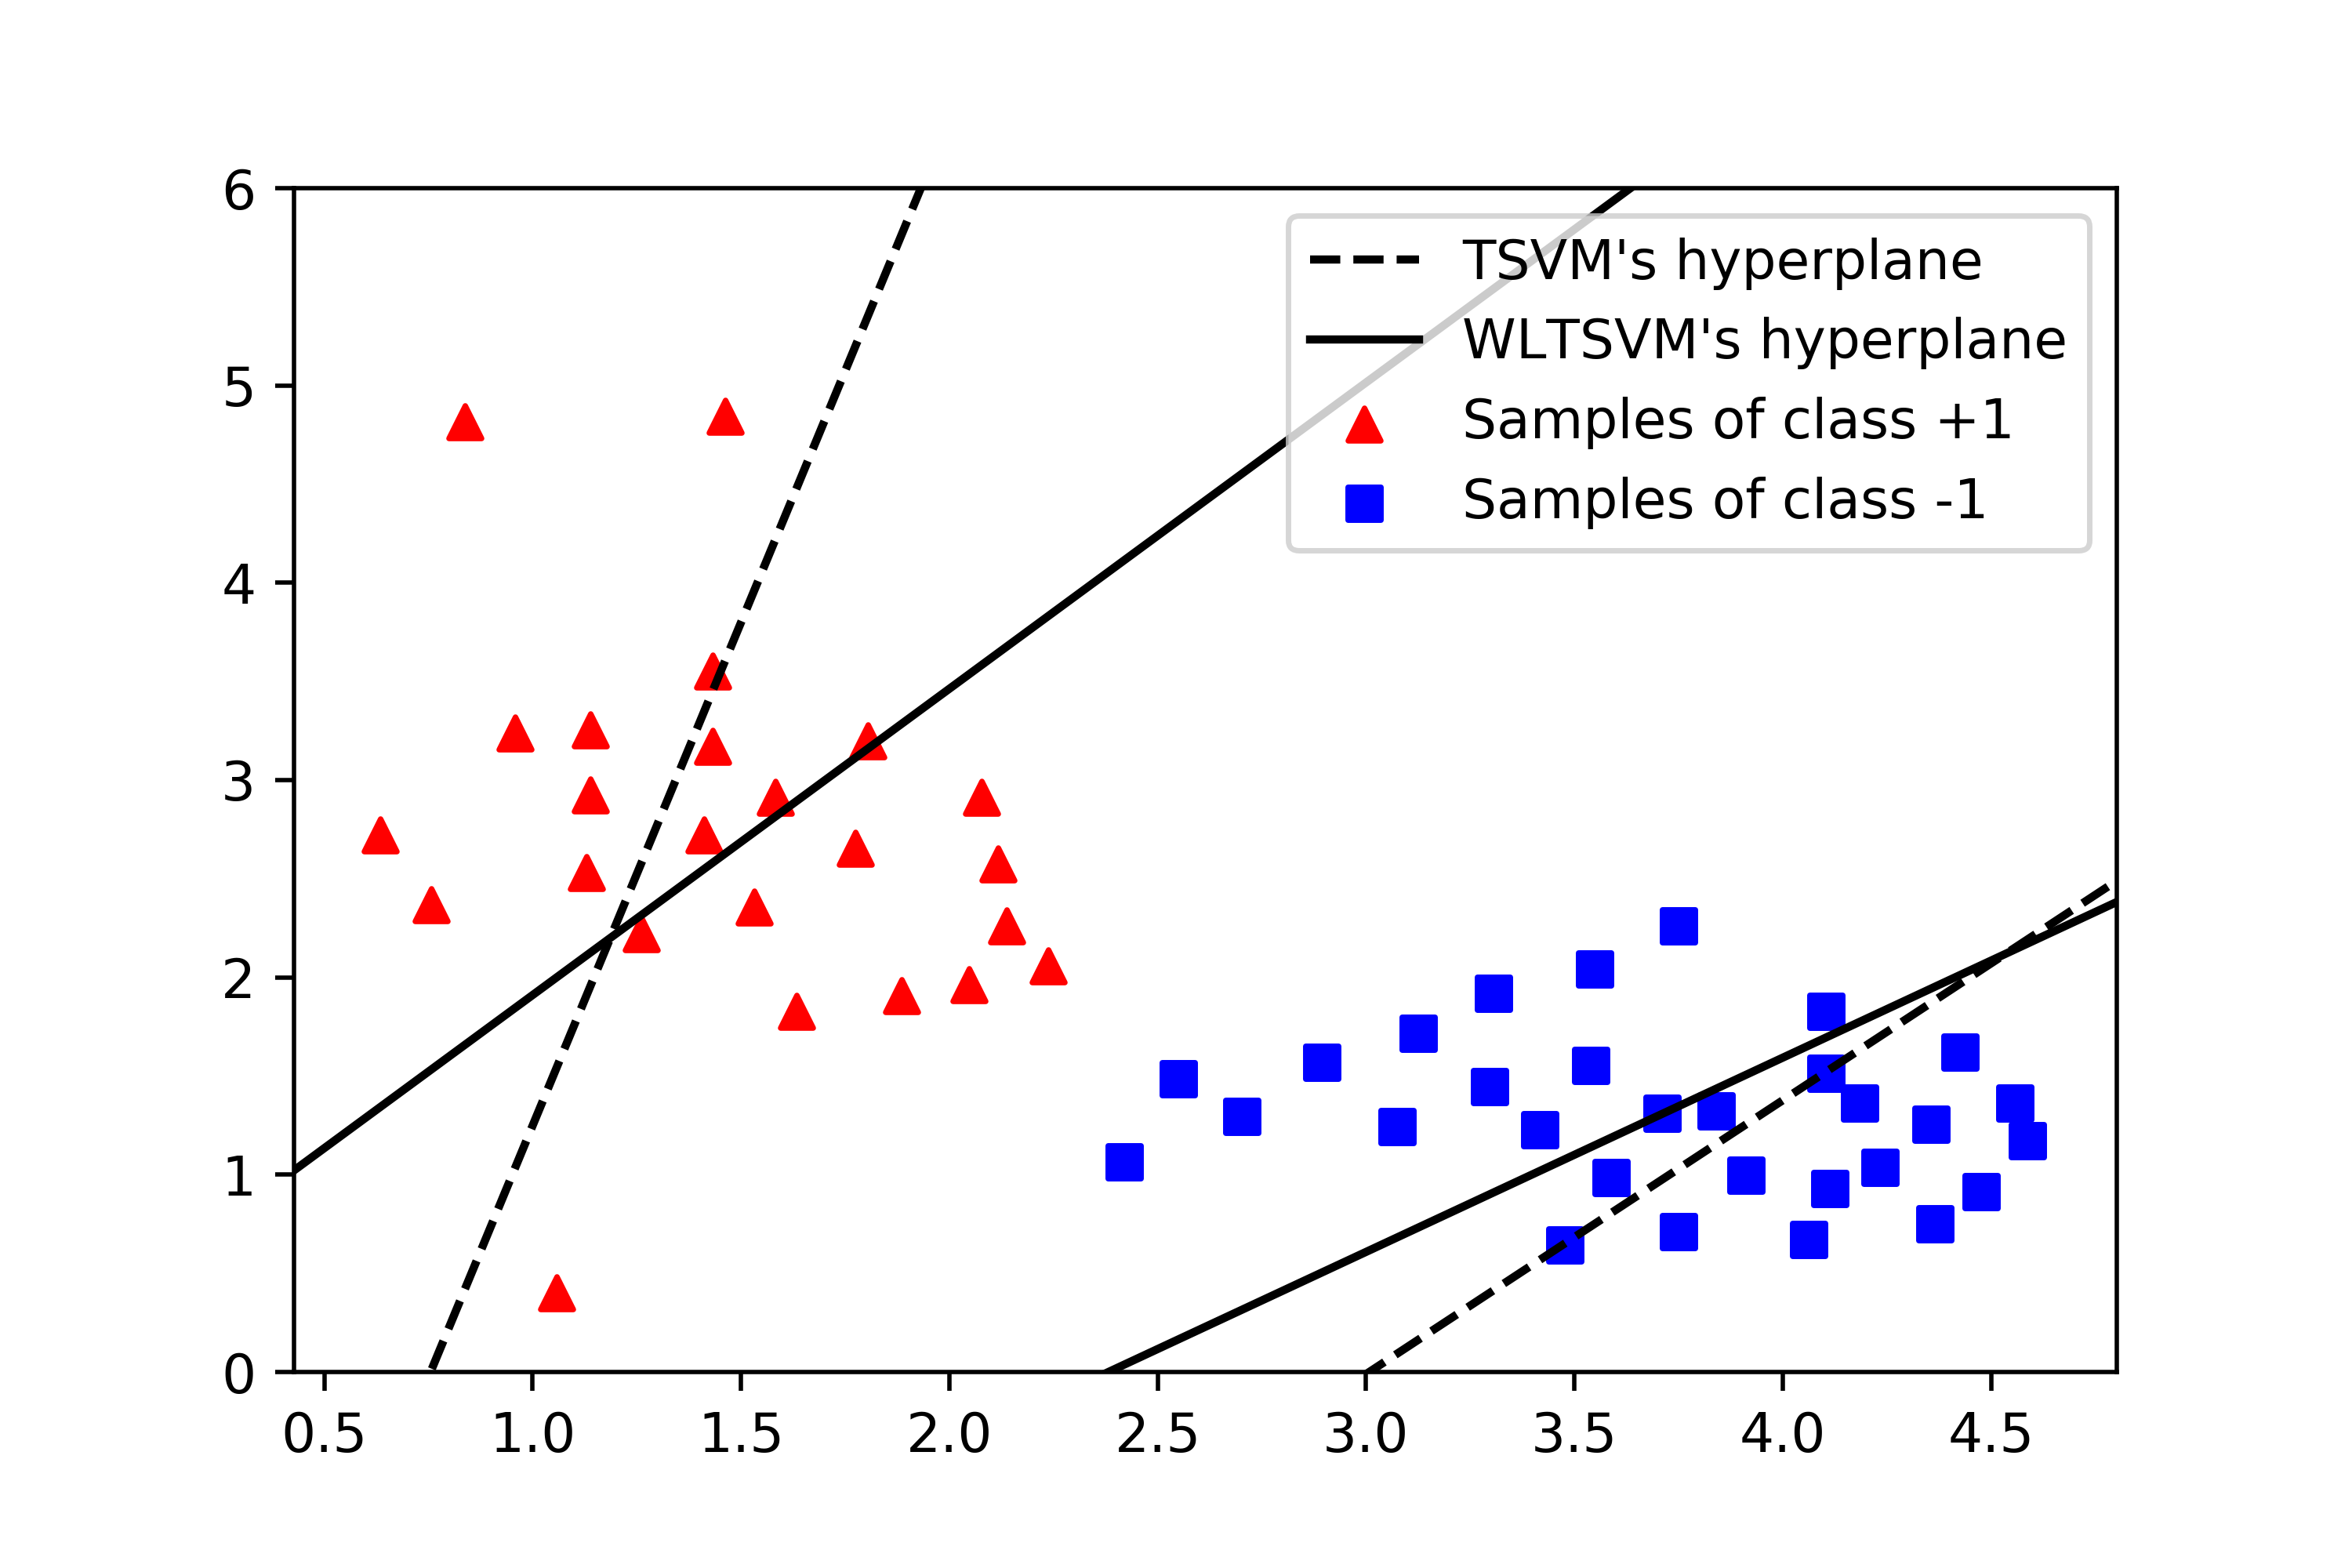
\includegraphics[scale=0.5]{TSVM-vs-WLTSVM}
	\caption{مقایسه هندسی روش \lr{WLTSVM} با روش \lr{TSVM} }
	\label{fig:TSVM-WLTSVM}
\end{figure}

همانطور که شکل ‏\ref{fig:TSVM-WLTSVM} در نشان داده شده است، ابرصفحه غیرموازی در روش \lr{WLTSVM} به نمونه‌های پرتراکم نزدیک‌تر و از نمونه‌های پرت فاصله بیشتری دارد. در این روش دو مسئله بهینه‌سازی اصلی به صورت زیر تعریف می‌شود.
\begin{equation}
\begin{split}
\mathop{{ min}}\limits_{w_{1} ,b_{1}} \qquad & \frac{1}{2}\sum\limits_{i=1}^{m_{1}}{\sum\limits_{j=1}^{m_{1}}{W^{(1)}_{s,ij}(w^{T}_{1}x^{(1)}_{j}+b_{1})^{2}}}+c\sum\limits_{j=1}^{m_{2}}\xi_j \\
\textrm{\lr{s.t. }} \qquad & -f^{(2)}_{j}(w^{T}_{1}x^{(2)}_{j}+b_{1})+\xi_{j} \ge f^{(2)}_{j} \\
& \xi_{j} \ge 0,\quad j=1,...,m_{2}
\end{split}
\label{eq:56}
\end{equation}
\begin{equation}
\begin{split}
\mathop{{ min}}\limits_{w_{2} ,b_{2}} \qquad & \frac{1}{2}\sum\limits_{i=1}^{m_{2}}{\sum\limits_{j=1}^{m_{2}}{W^{(2)}_{s,ij}(w^{T}_{2}x^{(2)}_{j}+b_{2})^{2}}}+c\sum\limits_{j=1}^{m_{1}}\eta_j \\
\textrm{\lr{s.t. }} \qquad & f^{(1)}_{j}(w^{T}_{2}x^{(1)}_{j}+b_{2})+\eta_{j} \ge f^{(1)}_{j} \\
& \eta_{j} \ge 0,\quad j=1,...,m_{2}
\end{split}
\label{eq:57}
\end{equation}
در روابط \ref{eq:56} و \ref{eq:57}،  $c$ پارامتر خطا،  $\xi$ و $\eta$ متغیر لغزش،  $W_{s,ij}^{(1)}$ و  $W_{s,ij}^{(2)}$ به ترتیب نشان دهنده گراف درون کلاسی کلاس مثبت و منفی است. همچنین  $f_{j}^{(1)}$ و $f_{j}^{(2)}$ به ترتیب بیانگر نمونه‌های حاشیه‌ای کلاس مثبت و منفی است. در اینجا نکته حائز اهمیت این است که در قید مسئله بهینه‌سازی فقط نمونه‌های حاشیه‌ای کلاس مقابل در نظر گرفته می‌شود. در حالی که در روش \lr{TSVM} اصلی، تمام نمونه‌های کلاس مقابل در قید مسئله بهینه‌سازی لحاظ شده است. در نتیجه با در نظر گرفتن نمونه‌های حاشیه‌ای، مرتبه زمانی روش \lr{WLTSVM} نسبت به \lr{TSVM} کاهش می‌یابد.

با استفاده از تابع لاگرانژ و شرایط \lr{KKT} حالت دوگان مسئله اصلی \ref{eq:56} و \ref{eq:57} در زیر تعریف شده است.
\begin{equation}
\begin{split}
\mathop{{ min}}\limits_{\alpha} \qquad & \frac{1}{2}{{\alpha }^{T}}(F^{T}G){{({{H}^{T}}DH)}^{-1}}{({G}^{T}F)}\alpha -e_{2}^{T}F\alpha  \\
\textrm{\lr{s.t. }} \qquad & 0{{e}_{2}}\le \alpha \le {{c}}{{e}_{2}}
\end{split}
\label{eq:58}
\end{equation}
\begin{equation}
\begin{split}
\mathop{{ min}}\limits_{\beta} \qquad & \frac{1}{2}{{\beta }^{T}}(P^{T}H){{({{G}^{T}}QG)}^{-1}}{({H}^{T}P)}\beta -e_{1}^{T}P\beta  \\
\textrm{\lr{s.t. }} \qquad & 0{{e}_{1}}\le \beta \le {{c}}{{e}_{1}}
\end{split}
\label{eq:59}
\end{equation}

در رابطه \ref{eq:58} و \ref{eq:59}،  $D=diag(d^{(1)}_{1},d^{(1)}_{2},\dots,d^{(1)}_{m_{1}})$ و  $Q=diag(d^{(2)}_{1},d^{(2)}_{2},\dots,d^{(2)}_{m_{2}})$ نشان دهنده ماتریس وزن کلاس مثبت و منفی است.  همچنین  $P=diag(f^{(1)}_{1},f^{(1)}_{2},\dots,f^{(1)}_{m_{1}})$  و $F=diag(f^{(2)}_{1},f^{(2)}_{2},\dots,f^{(2)}_{m_{2}})$ نشان دهنده نمونه‌های حاشیه‌ای کلاس مثبت و منفی است. بعد از حل کردن مسئله بهینه‌سازی دوگان، مدل خروجی با حل کردن روابط زیر بدست می‌آید.
\begin{equation}
\left[ \begin{matrix}
{{w}_{1}} \\
{{b}_{1}} \\
\end{matrix}\right]= -{{({{H}^{T}}DH)}^{-1}}{{G}^{T}}F\alpha
\label{eq:60}
\end{equation}
\begin{equation}
\left[ \begin{matrix}
{{w}_{2}} \\
{{b}_{2}} \\
\end{matrix}\right]= {{({{G}^{T}}QG)}^{-1}}{{H}^{T}}P\beta
\label{eq:61}
\end{equation}

نسخه غیر خطی روش \lr{WLTSVM} در مقاله اصلی شرح داده شده است \cite{ye2012}. روش \lr{WLTSVM} نسبت به \lr{TSVM} اصلی برتری‌های نظیر دقت دسته‌بندی بیشتر و مرتبه‌زمانی بهتر را دارد. با این حال روش \lr{WLTSVM} دارای نقاط ضعفی است که عبارتند از:
\begin{enumerate}
	\item روش  \lr{WLTSVM}به هر نمونه بر اساس تعداد نزدیک‌ترین همسایه‌هایش وزن نسبت می‌دهد. به عنوان مثال، وزن نمونه‌های کلاس مثبت از طریق رابطه زیر محاسبه می‌شود.
	\begin{equation}
	{{d}_{j}^{(1)}}=~\underset{i=1}{\overset{{{m}_{1}}}{\mathop \sum }}\,{{W}_{s,ij}}~,~j=1,2,\ldots ,{{m}_{1}}
	\label{eq:62}
	\end{equation}
	در رابطه \ref{eq:62}، متغیر $d_{j}^{(1)}$ نشان دهنده وزن نمونه $x_{j}$ است و  $W_{s,ij}$ مقدار 0 یا 1 دارد. در حالی که می‌توان به همسایه‌های یک نمونه مقداری بین 0 تا 1 براساس فاصله شان نسبت داد. 
	
	\item این روش نیز مانند \lr{TSVM} ریسک تجربی را در مسائل اصلی \ref{eq:56} و \ref{eq:57} کمینه می‌کند. بطوریکه برای جلوگیری از شرایط ماتریس منفرد، معکوس ماتریس‌های   $({H}^{T}DH)^{-1}$ و  $({G}^{T}QG)^{-1}$  به ترتیب با   $({H}^{T}DH + \varepsilon I)^{-1}$ و $({G}^{T}QG + \varepsilon I)^{-1}$  جایگزین میشود. بنابراین تنها راه حل تقریبی مسائل \ref{eq:58} و \ref{eq:59} بدست می‌آید.
	\item با وجود اینکه روش  \lr{WLTSVM} مرتبه زمانی را با لحاظ کردن نمونه‌های حاشیه‌ای در قید مسئله بهینه‌سازی کاهش می‌دهد. در این روش، \lr{k} تا از نزدیک‌ترین همسایه‌های تمام نمونه‌های آموزشی باید محاسبه شود. بنابراین پیچیدگی محاسباتی کلی این روش برابر با  $\mathcal{O}(2m_{1}^{3}+m^{2}logm)$ است. با فرض اینکه  $m_{1}=m_{2}$  و  $m_{1},m_{2} \ll m$. روش‌های جدید و سریع \lr{KNN} برای حل کردن این مشکل می‌تواند استفاده شود.
\end{enumerate}

\subsubsection{سایر گسترش‌های ماشین بردار پشتیبان دو قلو}\label{sec:2:2:3:4}
در این زیربخش، سایر روش‌های مبتنی بر \lr{TSVM} به طور خلاصه معرفی می‌شود. هر کدام از این از گسترش ها، یک نقطه ضعف روش \lr{TSVM} را حل کرده‌اند \cite{ding2014,ding2017,huang2018}. در سال 2013، ماشین بردار پشتیبان دو قلو ساختاری  \footnote{\lr{Structural Twin Support Vector Machine (STSVM)}}(\lr{STSVM}) ارائه گردید \cite{qi2013}.  این روش یادگیری اطلاعات مفید ساختاری درون هر کلاس و توزیع نمونه‌ها را از طریق خوشه‌بندی سلسله مراتبی در مدل خروجی لحاظ می‌کند.  

در سال 2014، ماشین بردار پشتیبان دو قلو مبتنی بر انرژی\footnote{\lr{Energy-based Model of Least Squares Twin Support Vector Machine (ELS-TSVM)}}  (\lr{ELS-TSVM}) ارائه شد \cite{nasiri2014}. در این روش، پارامتر انرژی برای دو ابرصفحه غیرموازی تعریف شده است. بطوریکه مقدار این پارامتر باتوجه به دانش قبلی تعیین می‌شود تا اثر نمونه‌های نویزی و پرت کاهش یابد. در سال 2015، ماشین بردار پشتیبان دو قلو ساختاری با رویکرد گراف نزدیک‌ترین همسایه (\lr{KNN-STSVM}) معرفی شد \cite{pan2015}. در این روش، علاوه بر در نظر گرفتن اطلاعات ساختاری نمونه‌ها، با استفاده از گراف نزدیک‌ترین همسایه به نمونه‌ها وزن داده می‌شود. در نتیجه، دقت مدل خروجی افزایش می‌یابد.

در سال 2016، ماشین بردار پشتیبان دو قلو چند کلاسه با رویکرد مبتنی بر نزدیک‌ترین همسایه\footnote{\lr{ K-nearest neighbor-based weighted multi-class twin support vector machine (KWM-TSVM)}}  (\lr{KWM-TSVM}) معرفی شد \cite{xu2016}. این روش با استفاده از گراف نزدیک‌ترین همسایه، اطلاعات درون کلاسی و برون کلاسی را در تابع هدف مسئله بهینه‌سازی لحاظ می‌کند. در نتیجه پیچیدگی زمانی و دقت مدل بهبود یافته است. در سال 2018، یک روش امن برای کاهش تعداد نمونه‌ها\footnote{\lr{Safe instance reduction rule}}  در روش \lr{KWM-TSVM } ارائه گردید \cite{pang2018}. این روش بخش زیادی از نمونه‌های دو کلاس را قبل از آموزش مدل حذف می‌کند. بنابراین پیچیدگی محاسباتی به طور قابل توجه‌ای کاهش یافته است. 

\begin{table}
	\small
	\centering
	\caption{مرور کلی گسترش‌های مبتنی بر روش  \lr{TSVM}}
	
	\begin{tabular}{c c p{8cm}}
		\hline
		روش یادگیری & سال معرفی & \multicolumn{1}{c}{ایده اصلی} \\
		\hline
		\lr{LS-TSVM} \cite{kumar2009} & 2009 & حل دستگاه معادلات خطی به جای مسئله دوگان که باعث افزایش چشم‌گیر سرعت یادگیری شده است. \\
		\lr{TBSVM} \cite{shao2011} & 2011 & ریسک ساختاری را در مسئله بهینه‌سازی خود کمینه می‌کند. همچنین از شرایط ماتریس منفرد جلوگیری می‌کند. \\
		\lr{WLTSVM} \cite{ye2012} & 2012 & با استفاده از گراف نزدیک‌ترین همسایه به هر نمونه وزن می‌دهد و نمونه‌های حاشیه‌ای هر کلاس را مشخص می‌کند. \\
		\lr{STSVM} \cite{qi2013} & 2013 & اطلاعات ساختاری را از طریق خوشه‌بندی سلسله مراتبی در مدل خروجی لحاظ می‌کند. \\
		\lr{ELS-TSVM} \cite{nasiri2014} & 2014 & پارامتر انرژی برای دو ابرصفحه معرفی شده است که اثر نمونه‌های نویزی و پرت را در مدل خروجی کمتر می‌کند. \\
		\lr{KNN-STSVM} \cite{pan2015} & 2015 & اطلاعات ساختاری با گراف نزدیک‌ترین همسایه برای بهبود دقت مدل خروجی ترکیب شده است. \\
		\lr{KWM-TSVM} \cite{xu2016} & 2016 & روش \lr{TSVM} چندکلاسه را با استفاده از گراف نزدیک‌ترین همسایه از تظر دقت و پیچیدگی زمانی بهبود داده است. \\
		\lr{SIR-KMTSVM} \cite{pang2018} & 2018 & بخش زیادی از نمونه‌های دو کلاس را با استفاده از یک قاعده امن حذف می‌کند. بطوریکه پیچیدگی زمانی روش \lr{TSVM} چند کلاسه بهبود یافته است. \\
		\hline
	\end{tabular}
\label{tab:2:1}
\end{table}


% Chapter 3 KNN-LSTSVM

\chapter{ماشین بردار پیشتیبان دو قلو کمترین مربعات مبتنی بر نزدیک‌ترین همسایه }\label{ch:3}
\section{مقدمه}\label{sec:3:1}
نقطه ضعف بزرگ روش \lr{TSVM} و \lr{LS-TSVM} این است که این روش‌ها اطلاعات شباهت  بین نمونه‌های آموزشی را در نظر نمی‌گیرند. به عبارت دیگر، به تمام نمونه‌های آموزشی اهمیت یکسانی داده می‌شود. بطوریکه نمونه‌های نویزی و پرت دقت مدل خروجی را روی داده‌های جدید کاهش می‌دهد. روش \lr{WLTSVM} این نقطه ضعف مهم را حل کرده است. این روش با ساخت گراف نزدیک‌ترین همسایه، اطلاعات درون و برون کلاسی را در تابع هدف مسئله بهینه‌سازی لحاظ کرده است. بطوریکه به هر یک از نمونه‌های آموزشی وزن نسبت می‌دهد و همچنین نمونه‌های حاشیه‌ای هر کلاس را استخراج می‌کند.

روش \lr{WLTSVM} مانند \lr{TSVM} اصلی، دو مسئله بهینه‌سازی دوگان از نوع برنامه‌ریزی درجه دو حل می‌کند. بطوریکه آموزش روش \lr{WLTSVM} بر روی مجموعه داده‌های بزرگ کند و زمان‌بر خواهد بود. در این فصل، با گرفتن ایده از روش‌های \lr{LS-TSVM} و \lr{WLTSVM}، روش جدید ماشین بردار پشتیبان دو قلو کمترین مربعات مبتنی بر رویکرد نزدیک‌ترین همسایه (\lr{KNN-LSTSVM}) ارائه می‌شود \cite{mir2018}. روش پیشنهادی دارای مزایای زیر است:

\begin{itemize}[label=$\bullet$]
	\item روش پیشنهادی (\lr{KNN-LSTSVM})، مشابه روش \lr{WLTSVM} به طور کامل از اطلاعات شباهت بین نمونه‌ها استفاده می‌کند. بطوریکه با ساخت گراف نزدیک‌ترین همسایه اطلاعات درون و برون کلاسی را در مسئله بهینه‌سازی لحاظ می‌کند. به عبارت دیگر، به هر نمونه آموزشی بر اساس شمارش تعداد نزدیک‌ترین همسایه‌هایش وزن داده می‌شود. همچنین نمونه‌های حاشیه‌ای هر کلاس نیز مشخص می‌گردد.
	\item روش پیشنهادی مشابه روش \lr{LS-TSVM}، دو دستگاه معادلات خطی برای بدست آوردن مدل خروجی حل می‌کند. این مزیت روش پیشنهادی را به یک الگوریتم ساده با پیچیدگی محاسباتی کمتر از \lr{WLTSVM} تبدیل می‌کند. به طور کلی، روش \lr{KNN-LSTSVM} نیازی به الگوریتم‌های بهینه‌سازی برای حل مسائل دوگان ندارد.
	\item روش پیشنهادی برخلاف روش \lr{LS-TSVM} نسبت به نمونه‌های پرت حساسیت کمتری دارد. زیرا با استفاده از گراف نزدیک‌ترین همسایه به نمونه‌های پرت و نویزی ورن کمتری نسبت داده می‌شود. بنابراین مدل خروجی دقت بهتری خواهد داشت.
\end{itemize}

در ادامه این فصل، ابتدا نحوه ساخت ماتریس وزن‌ها از طریق گراف \lr{k} نزدیک‌ترین همسایه شرح داده می‌شود. سپس نسخه خطی و غیر خطی روش \lr{KNN-LSTSVM} توضیح داده شده است.

\section{ساخت ماتریس وزن‌ها}\label{sec:3:2}
ایده اصلی روش پیشنهادی (\lr{KNN-LSTSVM}) و \lr{WLTSVM} این است که به نمونه‌های با تراکم بیشتر وزن بیشتری بدهد و از کلاس مقابل نمونه‌های حاشیه‌ای را مشخص کند. به عبارت دیگر، ابرصفحه غیرموازی در روش \lr{KNN-LSTSVM} به نمونه‌های پرتراکم نزدیک‌تر است و از نمونه‌های حاشیه‌ای کلاس مقابل حداکثر فاصله را می‌گیرد. شکل \ref{fig:KNN-LSTSVM-LSTSVM} تفسیر هندسی روش \lr{LS-TSVM} و \lr{KNN-LSTSVM} را نشان می‌دهد.

\begin{figure}[!b]
	\centering
	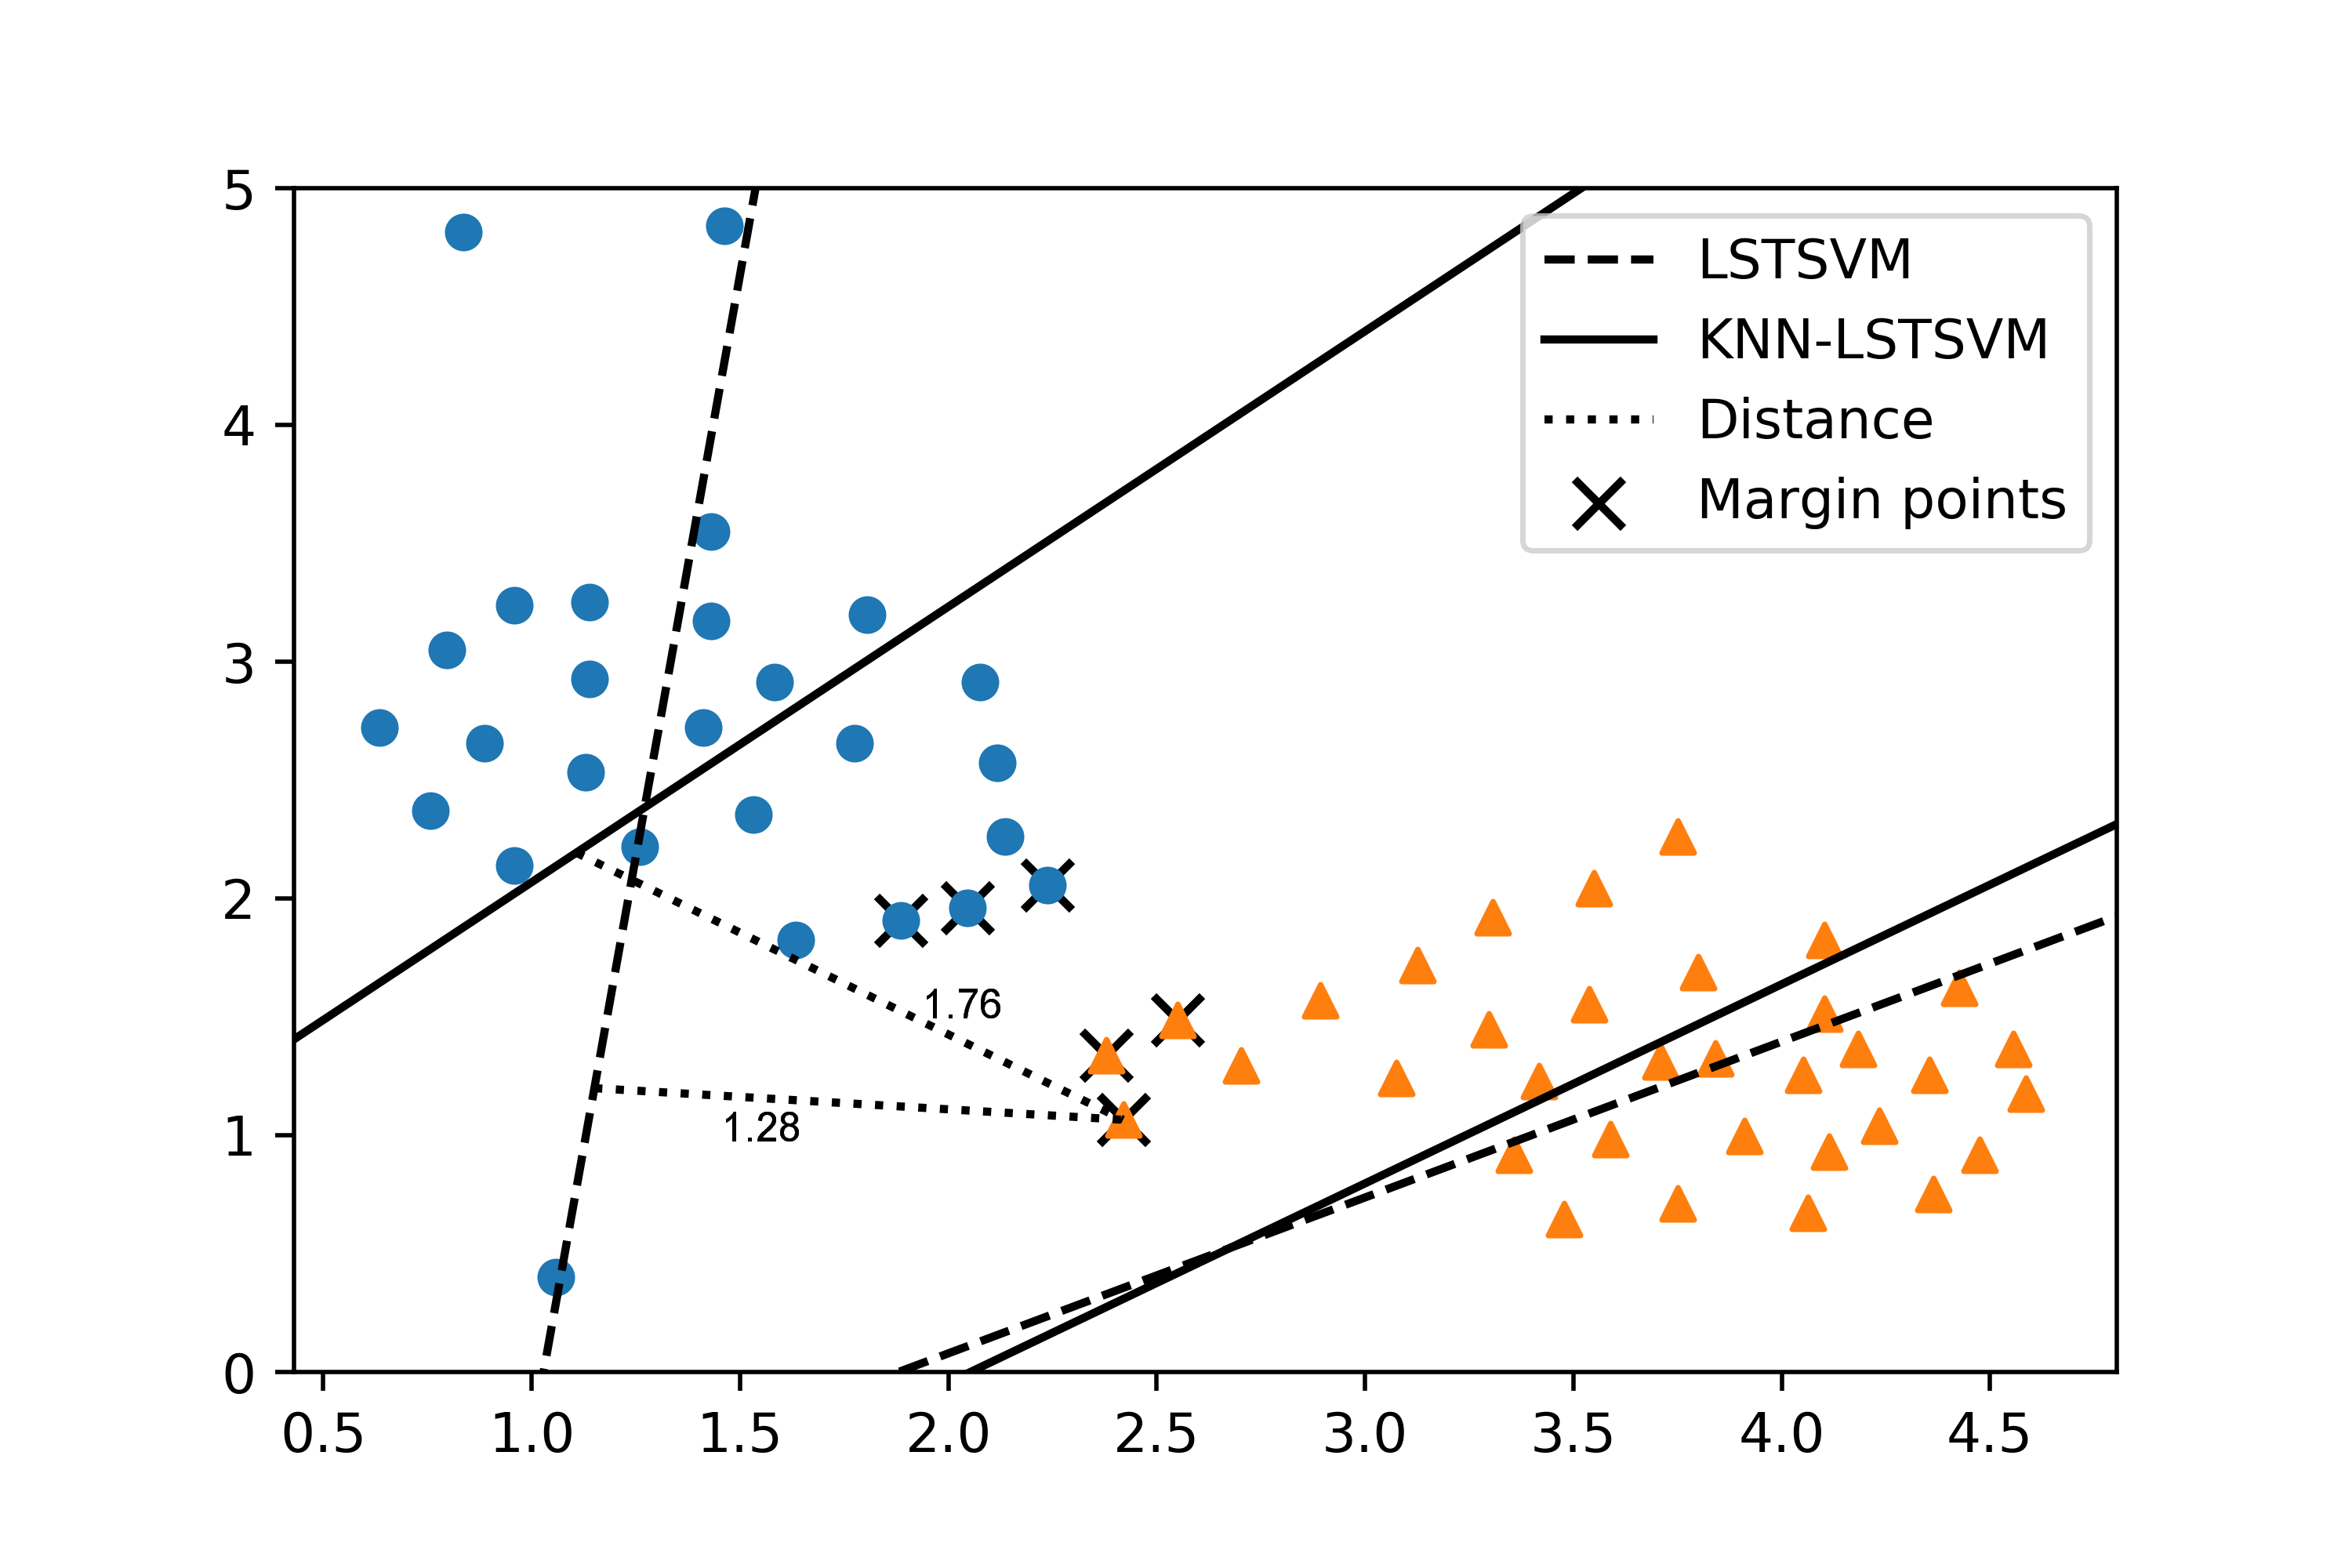
\includegraphics[scale=0.1]{KNN-LSTSVM-vs-LSTSVM}
	\caption{ تفسیر هندسی روش \lr{LS-TSVM} و \lr{KNN-LSTSVM}}
	\label{fig:KNN-LSTSVM-LSTSVM}
\end{figure}

همانطور که در شکل \ref{fig:KNN-LSTSVM-LSTSVM} مشخص شده است، ابرصفحه غیرموازی در \lr{LS-TSVM} به نمونه‌های پرت (کلاس دایره) بسیار نزدیک است. در حالی که روش پیشنهادی (\lr{KNN-LSTSVM}) از نمونه‌های پرت فاصله قابل توجه‌ای دارد و به نواحی پرتراکم نزدیک تر است. همچنین فاصله عمودی یک نمونه حاشیه‌ای از ابرصفحه هر دو روش در شکل ‏\ref{fig:KNN-LSTSVM-LSTSVM} محاسبه شده است. روش پیشنهادی از نمونه‌های حاشیه‌ای فاصله بیشتری دارد.

ابتدا گراف \lr{k} نزدیک‌ترین همسایه جهت بدست آوردن ماتریس وزن‌ها به صورت زیر تعریف می‌شود.
\begin{equation}\label{eq:63}
W_{ij} =
\begin{cases}
1, & \textrm{\lr{if }} x_i \in Nea\left(x_j\right)\textrm{\lr{ or }} x_j \in Nea\left(x_i\right),  \\
0, & \textrm{\lr{otherwise }}.
\end{cases}
\end{equation}

در رابطه \ref{eq:63}، مجموعه  شامل $k$ نزدیک‌ترین همسایه نمونه  $x_i$ است که در رابطه زیر تعریف شده است.
\begin{equation}\label{eq:64}
N(x_j) = \{x^1_j, x^2_j, \dots , x^k_j\}
\end{equation}

گراف $W$ به تنهایی نمی‌تواند تفکیک پذیری در داده‌ها را پیدا کند. در عوض یک گراف درون کلاسی  $W_{w,ij}$ و برون کلاسی   $W_{b,ij}$ ایجاد می‌شود تا به ترتیب فشردگی درون کلاسی\LTRfootnote{\lr{Intra-class compactness}}  و جداپذیری برون کلاسی\LTRfootnote{\lr{Inter-class separability}}  مشخص شود. ماتریس وزن $W_{w}$ و  $W_{b}$ به ترتیب در روابط \ref{eq:65} و \ref{eq:66} تعریف شده است.
\begin{equation}\label{eq:65}
W_{w,ij} =
\begin{cases}
1, & \textrm{\lr{if }} x_i \in N_w(x_j) \textrm{\lr{ or }} x_j \in N_w(x_i)  \\
0, & \textrm{\lr{otherwise }}.
\end{cases}
\end{equation}
\begin{equation}\label{eq:66}
W_{b,ij} =
\begin{cases}
1, & \textrm{\lr{if }} x_i \in N_b(x_j) \textrm{\lr{ or }} x_j \in N_b(x_i)  \\
0, & \textrm{\lr{otherwise}}.
\end{cases}
\end{equation}

در رابطه \ref{eq:65} و \ref{eq:66}، مجموعه $N_w(x_j)$ نشان‌دهنده $k$ نزدیک‌ترین همسایه نمونه $x_j$ از کلاس خودش و $N_b(x_j)$ مجموعه   شامل $k$ نزدیک‌ترین همسایه نمونه  $x_j$ از کلاس مقابل است. دو مجموعه $N_w(x_j)$ و $N_b(x_j)$ به ترتیب در روابط \ref{eq:67} و \ref{eq:68} تعریف شده‌اند.
\begin{align}
\label{eq:67}
\begin{split}
N_w\left(x_i\right) = \{x^j_i \mid l(x^j_i) = l(x_i), 1 \leq j \leq k \}
\end{split} \\
\label{eq:68}
\begin{split}
N_b\left(x_i\right) = \{x^j_i \mid l(x^j_i) \neq l(x_i), 1 \leq j \leq k \}
\end{split}
\end{align}

در رابطه \ref{eq:67} و \ref{eq:68}،  $l(x_i)$ نشان‌دهنده برچسب نمونه $x_i$ است. بدیهی است که  $N_w(x_i)\, \cap \, N_b(x_i) = \varnothing $ و  $N_w(x_i)\, \cup \, N_b(x_i) = N(x_i)$. فاصله بین هر کدام از نمونه‌های آموزشی توسط قاعده اقلیدس محاسبه می‌شود. به منظور پیدا کردن نمونه‌های حاشیه‌ای کلاس منفی، ماتریس وزن  $W_{b}$ به صورت زیر بازتعریف می‌شود.
\begin{equation}\label{eq:69}
f_{j} =
\begin{cases}
1, & \textrm{\lr{if }} \exists i, W_{b,ij} \neq 0  \\
0, & \textrm{\lr{otherwise}}.
\end{cases}
\end{equation}   

وزن هر کدام از نمونه‌های کلاس مثبت به صورت زیر محاسبه می‌شود.
\begin{equation}\label{eq:70}
{{d}_{j}}=~\underset{i=1}{\overset{{{m}_{1}}}{\mathop \sum }}\,{{W}_{w,~ij}}~,~j=1,2,\ldots ,~{{m}_{1}}
\end{equation}

در رابطه \ref{eq:70}، $d_j$  نشان‌دهنده وزن نمونه $x_j$ است. در اینجا تعداد همسایه‌ها با برچسب یکسان، وزن یک نمونه را مشخص می‌کند.

\section{نسخه خطی}\label{sec:2:3}
روش پیشنهادی مشابه روش \lr{WLTSVM}، دو ابرصفحه غیر موازی ایجاد می‌کند. بطوریکه هر کدام از این ابرصفحه‌ها به نمونه‌های پرتراکم نزدیک‌تر است و از نمونه‌های حاشیه‌ای کلاس مقابل حداکثر فاصله را دارد. با این حال روش پیشنهادی (\lr{KNN-LSTSVM})، مسائل اصلی روش \lr{WLTSVM} را تغییر می‌دهد. به این صورت که نامعادله در قید مسئله بهینه‌سازی به قید مساوی تغییر می‌یابد و همچنین متغیر لغزش به توان دو رسیده است.

راه حل دو مسئله اصلی تغییر یافته نیاز به حل کردن دو دستگاه معادلات خطی دارد. در حالی که در روش \lr{WLTSVM}، دو مسئله دوگان باید حل شود. مسئله اصلی تغییر یافته کلاس مثبت به صورت زیر تعریف می‌شود.
\begin{equation}\label{eq:71}
\begin{split}
\mathop{{ min}}\limits_{w_{(1)} ,b_{(1)}} \qquad & \frac{1}{2}{{(A{{w}^{\left( 1 \right)}}+e{{b}^{\left( 1 \right)}})}^{T}}D(A{{w}^{\left( 1 \right)}} +e{{b}^{\left( 1 \right)}}) +\frac{C}{2}{{y}^{T}}y \\
\textrm{\lr{s.t. }} \qquad & -F(B{{w}^{\left( 1 \right)}}+e{{b}^{\left( 1 \right)}})+y=Fe
\end{split}
\end{equation} 

 در رابطه \ref{eq:71}،  $D=diag(d_1,\dots,d_{m_{1}})$ نشان‌دهنده ماتریس وزن کلاس مثبت و $F=diag(f_1,\dots, f_{m_{2}})$ نشان دهنده نمونه‌های حاشیه‌ای کلاس منفی است. مقدار $f_j$ برابر با 0 یا 1 است و $d_i$ برزگتر یا مساوی با صفر است ($d_i \geq 0$).
 
 مزیت مهم مسئله اصلی \ref{eq:71} این است که که می‌توان قید مساوی را در آن در جایگذاری کرد. بنابراین تابع لاگرانژ مسئله اصلی \ref{eq:71} به صورت تعریف می‌شود.
\begin{equation}\label{eq:72}
 \mathop{{ min}}\limits_{w_{(1)} ,b_{(1)}} L = \quad \frac{1}{2}{{\left\| D(A{{w}^{(1)}}+{{e}}{{b}^{(1)}}) \right\|}^{2}} +{\frac{C}{2}}{{\left\|F( B{{w}^{(1)}}+{{e}}{{b}^{(1)}})+F{e} \right\|}^{2}}
\end{equation}

با گرفتن مشتق‌گیری جزئی از رابطه \ref{eq:72} نسبت به  $w^{(1)}$ و $b^{(1)}$  خواهیم داشت:
 \begin{align}
 \label{eq:73}
 \begin{split}
 \frac{\partial L}{\partial w^{(1)}} &= {{A}^{T}}D(A{{w}^{\left(1\right)}}+e{{b}^{\left( 1 \right)}} ) + C{{B}^{T}}F(B{{w}^{\left( 1 \right)}}+e{{b}^{\left( 1 \right)}}+Fe)=0e
 \end{split}\\
 \label{eq:74}
 \begin{split}
 \frac{\partial L}{\partial b^{(1)}} &= {{e}^{T}}D(A{{w}^{\left( 1 \right)}}+e{{b}^{\left( 1 \right)}}) + C{{e}^{T}}F(B{{w}^{\left( 1 \right)}}+e{{b}^{\left( 1 \right)}}+e)=0
 \end{split}
 \end{align}
 
 در ادامه با ترکیب کردن روابط \ref{eq:73} و \ref{eq:74} دستگاه معادلات خطی زیر بدست می‌آید.
 \begin{equation}\label{eq:75}
 \left[ \begin{matrix}
 {{B}^{T}}FB\, & {{B}^{T}}Fe  \\
 {{e}^{T}}FB\, & {{e}^{T}}Fe  \\
 \end{matrix} \right]\left[ \begin{matrix}
 {{w}^{\left( 1 \right)}}  \\
 {{b}^{\left( 1 \right)}}  \\
 \end{matrix} \right]+\frac{1}{C}\left[ \begin{matrix}
 {{A}^{T}}DA\, & {{A}^{T}}De  \\
 {{e}^{T}}DA\, & {{e}^{T}}De  \\
 \end{matrix} \right]\left[ \begin{matrix}
 {{w}^{\left( 1 \right)}}  \\
 {{b}^{\left( 1 \right)}}  \\
 \end{matrix} \right] +\left[ \begin{matrix}
 {{B}^{T}}Fe  \\
 {{e}^{T}}Fe  \\
 \end{matrix} \right]=0e.
 \end{equation}
 \begin{equation}\label{eq:76}
 \left[ \begin{matrix}
 {{w}^{\left( 1 \right)}}  \\
 {{b}^{\left( 1 \right)}}  \\
 \end{matrix} \right]={{\left[ \begin{matrix}
 		{{B}^{T}}FB+~\frac{1}{C}{{A}^{T}}DA\, & {{B}^{T}}Fe+\frac{1}{C}{{A}^{T}}De\,  \\
 		{{e}^{T}}FB+~\frac{1}{C}{{e}^{T}}DA\, & {{e}^{T}}Fe+\frac{1}{C}{{e}^{T}}De\,  \\
 		\end{matrix} \right]}^{-1}} \times \left[ \begin{matrix}
 -{{B}^{T}}Fe  \\
 -{{e}^{T}}Fe  \\
 \end{matrix} \right]
 \end{equation}
 \begin{equation}\label{eq:77}
 \left[ \begin{matrix}
 {{w}^{\left( 1 \right)}}  \\
 {{b}^{\left( 1 \right)}}  \\
 \end{matrix} \right]={{\left[ \begin{matrix}
 		\left[ \begin{matrix}
 		{{B}^{T}}  \\
 		{{e}^{T}}  \\
 		\end{matrix} \right]F & \left[ \begin{matrix}
 		B & e  \\
 		\end{matrix} \right]+~\frac{1}{C}\left[ \begin{matrix}
 		{{A}^{T}}  \\
 		{{e}^{T}}  \\
 		\end{matrix} \right]D\left[ \begin{matrix}
 		A & e  \\
 		\end{matrix} \right]  \\
 		\end{matrix} \right]}^{-1}} \times \left[ \begin{matrix}
 \left[ \begin{matrix}
 -{{B}^{T}}  \\
 -{{e}^{T}}  \\
 \end{matrix} \right] & Fe  \\
 \end{matrix} \right]
 \end{equation}
 
با تعریف کردن ماتریس $H$ و $G$ به صورت $H=[A\text{ }e]$ و $G=[B\text{ }e]$، راه حل مسئله بهینه‌سازی \ref{eq:71} به صورت زیر تعریف می‌شود.
\begin{equation}\label{eq:78}
\left[ \begin{matrix}
{{w}^{\left( 1 \right)}}  \\
{{b}^{\left( 1 \right)}}  \\
\end{matrix} \right] = -{{({{G}^{T}}FG+\frac{1}{C}{{H}^{T}}DH)}^{-1}}{{G}^{T}}Fe
\end{equation}

مسئله اصلی تغییر یافته کلاس منفی به صورت زیر تعریف می‌شود.
\begin{equation}\label{eq:79}
\begin{split}
\mathop{{ min}}\limits_{w_{(2)} ,b_{(2)}} \qquad & \frac{1}{2}{{(B{{w}^{\left( 2 \right)}}+e{{b}^{\left( 2 \right)}})}^{T}}Q(B{{w}^{\left( 2 \right)}}+e{{b}^{\left( 2 \right)}})+\frac{C}{2}{{y}^{T}}y \\
\textrm{\lr{s.t. }} \qquad & P(A{{w}^{\left( 2 \right)}}+e{{b}^{\left( 2\right)}})+y=Pe
\end{split}
\end{equation}

در رابطه \ref{eq:79}،  $Q=diag(q_1,\dots,q_{m_{2}})$ نشان‌دهنده ماتریس وزن کلاس منفی و  $P=diag(p_1,\dots  ,p_{m_{1}})$ نشان‌دهنده نمونه‌های حاشیه‌ای کلاس مثبت است. مانند ماتریس $F$، مقدار $p_j$  برابر 0 یا 1 است.

راه حل مسئله اصلی \ref{eq:79} همانند کلاس مثبت با جایگذاری قید مساوی، گرفتن مشتق‌گیری جزئی به صورت زیر تعریف می‌شود.
\begin{equation}\label{eq:80}
\left[ \begin{matrix}
{{w}^{\left( 2 \right)}}  \\
{{b}^{\left( 2 \right)}}  \\
\end{matrix} \right] = {{({{H}^{T}}PH+\frac{1}{C}{{G}^{T}}QG)}^{-1}}{{H}^{T}}Pe
\end{equation}

راه حل‌های \ref{eq:78} و \ref{eq:80} شامل دو معکوس ماتریس با اندازه $(n+1)\times (n +1)$ است. بطوریکه $n$ بسیار کوچکتر از تعداد نمونه‌های کلاس مثبت و منفی می‌باشد. بنابراین سرعت یادگیری نسخه خطی روش \lr{KNN-LSTSVM} بسیار زیاد است.

تابع تصمیم نسخه خطی به صورت زیر تعریف می‌شود.
\begin{equation}\label{eq:81}
D(x_i) =
\begin{cases}
+1, & \textrm{\lr{if }} |{{x}^T}{{w}^{(1)}}+{{b}^{(1)}}|\, < \, |{{x}^T}{{w}^{(2)}}+{{b}^{(2)}}|  \\
-1, & \textrm{\lr{otherwise }}.
\end{cases}
\end{equation}

مراحل ایجاد مدل خطی روش \lr{KNN-LSTSVM} در الگوریتم \ref{Algo:Linear-KNN-LSTSVM} خلاصه شده است.
\\
\begin{algorithm}[h]
\begin{steps}

 	ابتدا فرض می‌گیریم که نمونه‌های کلاس مثبت با ماتریس  $A\in {{\mathbb{R}}^{{{m}_{1}}\times n}}$ و نمونه‌های کلاس منفی با ماتریس  $B\in {{\mathbb{R}}^{{{m}_{2}}\times n}}$ نشان داده شده است.
 	
 	\begin{enumerate}
 		\item ابتدا پارامتر  $k$ برای ساخت گراف نزدیک‌ترین همسایه تعیین می‌شود. سپس ماتریس وزن‌های  $W_{w}$ و   $W_{b}$ برای کلاس مثبت و منفی با استفاده از روابط \ref{eq:65} و \ref{eq:66} بدست می‌آید.
 		\item ماتریس‌های قطری  $D$،$F$ ،$Q$  و $P$ باید تعریف گردد. سپس ماتریس‌های $H$ و  $G$ به صورت  $H=[A\text{ } e]$ و $G=[B\text{ }e]$  تعریف می‌شود.
 		\item مقدار پارامتر خطا $C$ باید تعیین گردد. این پارامتر معمولا براساس \gls{Vset} مشخص می‌شود.
 		\item مختصات دو ابرصفحه غیرموازی از طریق روابط \ref{eq:78} و \ref{eq:80} بدست می‌آید.
 		\item فاصله عمودی از $|{{x}^T}{{w}^{(1)}}+{{b}^{(1)}}|$  و  $|{{x}^T}{{w}^{(2)}}+{{b}^{(2)}}|$ برای نمونه جدید   $x \in \mathbb{R}^{n}$ محاسبه می‌شود.
 		\item کلاس نمونه جدید از طریق تابع تصمیم \ref{eq:81} مشخص می‌گردد.
 	\end{enumerate}
\end{steps}
\caption{ ایجاد مدل خطی روش \lr{KNN-LSTSVM}}
\label{Algo:Linear-KNN-LSTSVM}
\end{algorithm}
 
\section{نسخه غیر خطی}\label{sec:3:3}
به منظور حل کردن مسائل غیر خطی، نسخه خطی روش \lr{KNN-LSTSVM} با در نظرگرفتن دو ابرسطح  زیر می‌توان به نسخه غیر خطی گسترش داد.
\begin{equation}\label{eq:82}
K({{x}^{T}},~{{C}^{T}}){{u}^{\left( 1 \right)}}+{{b}^{\left( 1 \right)}}=0 \text{\lr{ and }} K({{x}^{T}},~{{C}^{T}}){{u}^{\left( 2 \right)}}+{{b}^{\left( 2 \right)}}=0
\end{equation}

در رابطه \ref{eq:82}، ماتریس برابر $C$ با  $C=\left[ A \  B \right]^{T}$ است و $K$  تابع هسته دلخواه می‌باشد. همانند نسخه خطی، مسائل بهینه‌سازی اصلی نسخه غیر خطی روش  \lr{KNN-LSTSVM} با مساوی قرار دادن قید برای کلاس مثبت و منفی به ترتیب در روابط \ref{eq:83} و \ref{eq:84} تعریف شده است.
\begin{align}
\mathop{{ min}}\limits_{u_{(1)} ,b_{(1)}} \quad & \frac{1}{2}{{(K(A,~{{C}^{T}}){{u}^{\left( 1 \right)}}+e{{b}^{\left( 1 \right)}})}^{T}}D(K( A,~{{C}^{T}}){{u}^{\left( 1 \right)}} \nonumber +e{{b}^{\left( 1 \right)}}) +\frac{C}{2}{{y}^{T}}y \nonumber \\
\textrm{\lr{s.t. }} \quad & 	-F(K(B,~{{C}^{T}}){{u}^{\left( 1 \right)}}+e{{b}^{\left( 1 \right)}})+y=Fe
\label{eq:83}
\end{align}
\begin{align}
\mathop{{ min}}\limits_{u_{(2)} ,b_{(2)}} \quad & \frac{1}{2}{{(K(B,{{C}^{T}}){{u}^{(2)}}+e{{b}^{(2)}})}^{T}}Q(K(B,{{C}^{T}}){{u}^{(2)}} \nonumber +e{{b}^{(2)}})+\frac{C}{2}{{y}^{T}}y \nonumber \\
\textrm{\lr{s.t. }} \quad & P(K(A,{{C}^{T}}){{u}^{(2)}}+e{{b}^{(2)}})+y=Pe
\label{eq:84}
\end{align}

در روابط \ref{eq:83} و \ref{eq:84}، ماتریس  $K(A,{{C}^{T}})$ و $K(B,{{C}^{T}})$  نشان‌دهنده ماتریس هسته به ترتیب با اندازه‌های  $m_1 \times m$ و  $m_2 \times m$ هستند $(m=m_1+m_2)$. مسائل بهینه‌سازی اصلی \ref{eq:83} و \ref{eq:84} با جایگذاری قید در تابع هدف به صورت زیر تعریف می‌شود.
\begin{equation}\label{eq:85}
\begin{split}
\mathop{{ min}}\limits_{u_{(1)} ,b_{(1)}}~ & \frac{1}{2}\left\|D(K(A,~{{C}^{T}}){{u}^{\left( 1 \right)}}+e{{b}^{\left( 1 \right)}})\right\|^{2} +\frac{C}{2}\left\|F(K(B,~{{C}^{T}}){{u}^{\left( 1 \right)}}+e{{b}^{\left( 1 \right)}}+F{{e}})\right\|^{2}
\end{split}
\end{equation}
\begin{equation}\label{eq:86}
\begin{split}
\mathop{{ min}}\limits_{u_{(2)} ,b_{(2)}}~ & \frac{1}{2}\left\|Q(K(B,~{{C}^{T}} ){{u}^{\left( 2 \right)}}+e{{b}^{\left( 2 \right)}})\right\|^{2} +\frac{C}{2}\left\|P(K(A,~{{C}^{T}} ){{u}^{\left( 2 \right)}}+e{{b}^{\left( 2 \right)}}+P{{e}})\right\|^{2}
\end{split}
\end{equation}

راه حل مسائل \ref{eq:85} و \ref{eq:86} به طرز مشابه نسخه خطی در زیر تعریف شده است.
\begin{align}
\left[\begin{matrix}
{{u}^{(1)}}  \\
{{b}^{(1)}}  \\
\end{matrix} \right]= & -{({{S}^{T}}FS+\frac{1}{C}{{R}^{T}}DR)^{-1}}{{S}^{T}}Fe \label{eq:87} \\
\left[ \begin{matrix}
{{u}^{(2)}}  \\
{{b}^{(2)}}  \\
\end{matrix} \right]= & {({{R}^{T}}PR+\frac{1}{C}{{S}^{T}}QS)^{-1}}{{R}^{T}}Pe \label{eq:88}
\end{align}

در رابطه \ref{eq:87} و \ref{eq:88}، ماتریس $R$ و $S$  به صورت  $R=\left[ \begin{matrix} K(A,{{C}^{T}})\ & e  \\ \end{matrix} \right]$ و   $S=\left[ \begin{matrix} K(B,{{C}^{T}})\ & e  \\ \end{matrix} \right]$ تعریف می‌شود. کلاس یک نمونه جدید مشابه نسخه خطی تعیین می‌شود. بطوریکه فاصله عمودی از دو ابرسطح محاسبه می‌گردد. تابع تصمیم در نسخه غیر خطی به صورت زیر تعریف شده است. 
\begin{equation}\label{eq:89}
D(x) =
\begin{cases}
+1, & \textrm{\lr{if }} |K(x,{C}^{T}){{u}^{(1)}}+{{b}^{(1)}}|\, < \, |K(x,{C}^{T}){{u}^{(2)}}+{{b}^{(2)}}|  \\
-1, & \textrm{\lr{otherwise}}.
\end{cases}
\end{equation}

لازم به ذکر است که راه حل نسخه غیر خطی روش \lr{KNN-LSTSVM} شامل دو معکوس ماتریس با ابعاد  $(m+1)\times (m+1)$ است. بطوریکه $m$  تعداد کل نمونه‌های آموزشی است. جهت کاهش پیچیدگی محاسباتی، می‌توان از فرمول \gls{SMW}  استفاده کرد \cite{golub2012}. در این صورت راه حل‌های \ref{eq:87} و \ref{eq:88} را می‌توان با چهار عمل معکوس ماتریس با ابعاد کوچک‌تر از $(m+1)\times (m+1)$ محاسبه کرد. 

بنابراین راه حل‌های \ref{eq:87} و \ref{eq:88} به صورت زیر بازنویسی می‌شود.
\begin{align}
\left[ \begin{matrix}
{{u}^{(1)}}  \\
{{b}^{(1)}}  \\
\end{matrix} \right]& = -(Y-Y{{R}^{T}}D{{(CI+RY{{R}^{T}}D)}^{-1}}RY){{S}^{T}}Fe \label{eq:90} \\
\left[ \begin{matrix}
{{u}^{(2)}}  \\
{{b}^{(2)}}  \\
\end{matrix} \right] & = (Z-Z{{S}^{T}}Q{{(CI+SZ{{S}^{T}}Q)}^{-1}}SZ){{R}^{T}}Pe \label{eq:91}
\end{align}

در رابطه \ref{eq:90} و \ref{eq:91}، ماتریس‌های $Y$ و $Z$  به صورت  $Y={{({{S}^{T}}FS)}^{-1}}$ و  $Z={{({{R}^{T}}PR)}^{-1}}$ تعریف می‌شوند. با این حال ماتریس‌های $({{S}^{T}}FS)$ و $({{R}^{T}}PR)$  ممکن که دچار شرایط منفرد شوند. یک عدد ثابت بسیار کوچک  $\varepsilon I$ , $\varepsilon > 0$ به این ماتریس‌ها اضافه می‌شود تا از شرایط منفرد جلوگیری شود. بعد از اضافه شدن $\varepsilon I$، می‌توان از \lr{SMW} برای پیدا کردن ماتریس‌های $Y$ و $Z$ به صورت زیر استفاده کرد.
\begin{align}
Y&= \frac{1}{\varepsilon }(I-{{S}^{T}}F{{(\varepsilon I+S{{S}^{T}}F)}^{-1}}S) \label{eq:92} \\
Z&= \frac{1}{\varepsilon }(I-{{R}^{T}}P{{(\varepsilon I+R{{R}^{T}}P)}^{-1}}R) \label{eq:93}
\end{align}

بعد از استفاده کردن از فرمول \lr{SMW}، راه حل نسخه غیر خطی شامل دو معکوس ماتریس به اندازه  $(m_1 \times m_1)$ و دو معکوس ماتریس به اندازه $(m_2 \times m_2)$  می‌شود. مراحل ایجاد مدل غیر خطی روش \lr{KNN-LSTSVM} در الگوریتم \ref{Algo:Non-Linear-KNN-LSTSVM} خلاصه شده است.

\begin{algorithm}[!t]
\begin{steps}
	
	ابتدا فرض می‌گیریم که نمونه‌های کلاس مثبت با ماتریس  $A\in {{\mathbb{R}}^{{{m}_{1}}\times n}}$ و نمونه‌های کلاس منفی با ماتریس  $B\in {{\mathbb{R}}^{{{m}_{2}}\times n}}$ نشان داده شده است.
	
	\begin{enumerate}
		\item ابتدا یک تابع هسته برای نگاشت نمونه‌های آموزشی به فضای ویژگی انتخاب می‌شود. غالبا از تابع \lr{RBF} در این مرحله استفاده می‌شود.
		\item ابتدا پارامتر  $k$ برای ساخت گراف نزدیک‌ترین همسایه تعیین می‌شود. سپس ماتریس وزن‌های  $W_{w}$ و   $W_{b}$ برای کلاس مثبت و منفی با استفاده از روابط \ref{eq:65} و \ref{eq:66} بدست می‌آید.
		\item ماتریس‌های قطری  $D$،$F$ ،$Q$  و $P$ باید تعریف گردد. سپس ماتریس‌های $R$ و  $S$ به صورت  $R=\left[ \begin{matrix} K(A,{{C}^{T}})\ & e  \\ \end{matrix} \right]$  و $S=\left[ \begin{matrix} K(B,{{C}^{T}})\ & e  \\ \end{matrix} \right]$  تعریف می‌شود.
		\item مقدار پارامتر خطا $C$ باید تعیین گردد. این پارامتر معمولا براساس مجموعه داده صحت  مشخص می‌شود.
		\item مختصات دو ابرسطح از طریق روابط \ref{eq:90} و \ref{eq:91} بدست می‌آید.
		\item فاصله عمودی از $|K(x,{C}^{T}){{u}^{(1)}}+{{b}^{(1)}}|$ و  $|K(x,{C}^{T}){{u}^{(2)}}+{{b}^{(2)}}|$ برای نمونه جدید  $x \in \mathbb{R}^{n}$ محاسبه می‌شود.
		\item کلاس نمونه جدید از طریق تابع تصمیم \ref{eq:89} مشخص می‌گردد.
	\end{enumerate}
\caption{ ایجاد مدل غیر خطی روش \lr{KNN-LSTSVM}}
\label{Algo:Non-Linear-KNN-LSTSVM}
\end{steps}
\end{algorithm}

\section{تحلیل روش \lr{KNN-LSTSVM}}\label{sec:3:4}
در مقایسه با \lr{LSTSVM}، روش پیشنهادی با استفاده از گراف نزدیک‌ترین همسایه اطلاعات درون کلاسی و برون کلاسی را در مسئله بهینه‌سازی لحاظ می‌کند. بنابراین روش \lr{KNN-LSTSVM} حساسیت کمتری نسبت به نمونه‌های نویزی و پرت دارد. همچنین روش پیشنهادی مانند \lr{LSTSVM} دو دستگاه معادلات خطی حل می‌کند. در نتیجه سرعت یادگیری هر دو روش بسیار زیاد است.

دو روش \lr{WLTSVM } و \lr{KNN-LSTSVM} با ساخت گراف نزدیک‌ترین همسایه به نمونه‌های آموزشی وزن می‌دهند و همچنین نمونه‌های حاشیه‌ای هر دو کلاس را مشخص می‌کنند. با این حال روش پیشنهادی دو دستگاه معادلات خطی حل می‌کند. در حالی که در \lr{WLTSVM} دو مسئله دوگان حل می‌شود. بنابراین سرعت یادگیری روش پیشنهادی بسیار بیشتر از \lr{WLTSVM} است.

با وجود اینکه مدل خروجی در روش پیشنهادی دقت بیشتری نسبت به \lr{LSTSVM} دارد، دو محدودیت مهم نیز دارد که عبارتند از:
\begin{enumerate}
	\item در راه‌های حل نسخه خطی و غیر خطی، عمل معکوس کردن ماتریس اجتناب ناپذیر است. از طرفی، مرتبه زمانی معکوس کردن ماتریس برابر با  $\mathcal{O}({{m}^{3}})$ است. بنابراین زمان محاسبه با افزایش ابعاد ماتریس، به طور قابل توجه‌ای بیشتر می‌شود.
	\item مصرف حافظه روش پیشنهادی برای مجموعه داده‌های بزرگ (بیش از 50 هزار نمونه) بسیار زیاد است. زیرا دو گراف نزدیک‌ترین همسایه و ماتریس وزن‌ها برای ساخت مدل باید ذخیره گردد.
\end{enumerate}

\section{جمع‌بندی}\label{sec:3:5}
در این فصل دسته‌بند \lr{KNN-LSTSVM } ارائه شد. روش پیشنهادی همانند \lr{WLTSVM} با ساخت گراف نزدیک‌ترین همسایه، به نمونه‌های آموزشی وزن می‌دهد و نمونه‌های حاشیه‌ای هر کلاس را مشخص می‌کند. ایده اصلی روش پیشنهادی این است که ابرصفحه غیر موازی به نمونه‌های پرتراکم کلاس خود نزدیک می‌شود و از نمونه‌های حاشیه‌ای کلاس مقابل حداکثر فاصله را می‌گیرد. با این حال دسته‌بند \lr{KNN-LSTSVM} مزیت اصلی روش \lr{LSTSVM} دارد. بطوریکه دو دستگاه معادلات خطی برای ساخت مدل خروجی حل می‌شود. همچنین نقطه ضعف روش \lr{LSTSVM} یعنی حساسیت به نمونه‌های نویزی و پرت در روش پیشنهادی برطرف شده است. روش \lr{KNN-LSTSVM} در بخش \ref{sec:5:2} به طور جامع ارزیابی شده است.

روش \lr{KNN-LSTSVM} در مجله زیر به چاپ رسیده است.
\begin{LTR}
\begin{itemize}[label=$\bullet$]
	\item \lr{KNN-based least squares twin support vector machine for pattern classification, Applied Intelligence (2018): 1-14}
\end{itemize}
\end{LTR}


% Chapter 4 RKNN-TSVM

\chapter{ماشین بردار پشتیبان دو قلو مبتنی بر رگولارسیون و نزدیک‌ترین همسایه}\label{ch:4}
\section{مقدمه}\label{sec:4:1}
در بخش ‏\ref{sec:2:2:3} برخی از گسترش‌های \lr{TSVM} معرفی شد. بعضی از این گسترش‌ها مبتنی بر رویکرد نزدیک‌ترین همسایه هستند. با وجود اینکه گسترش‌های با رویکرد نزدیک‌ترین همسایه مزیت‌هایی مانند دقت بیشتر را دارند، این روش‌ها سه نقطه ضعف دارند که عبارتند از:
\begin{enumerate}
	\item این روش‌ها به نمونه‌ها بر اساس شمارش تعداد همسایه‌های نزدیک‌شان وزن می‌دهند. بطوریکه فاصله بین نزدیک‌ترین همسایه‌های یک نمونه در نظر گرفته نمی‌شود. نسبت دادن وزن براساس فاصله می‌تواند باعث شناسایی بهتر نواحی پرتراکم شود. به عبارت دیگر، وزن بیشتری به یک نمونه با همسایه‌های نزدیک‌تر داده می‌شود تا به یک نمونه با همسایه‌های دورتر.
	\item این روش‌ها همانند \lr{TSVM} خطای آموزشی (ریسک تجربی) را کمینه می‌کنند. از این رو امکان برازش بیش از حد وجود دارد و تعمیم‌پذیری مدل خروجی کاهش می‌یابد. این نقطه ضعف با در نظر گرفتن ریسک ساختاری در تابع هدف مسئله بهینه‌سازی برطرف می‌شود.
	\item در این روش‌ها، گراف نزدیک‌ترین همسایه با الگوریتم جستجوی کامل\footnote{\lr{Full search algorithm}}  (\lr{FSA}) ساخته می‌شود. مرتبه زمانی این الگوریتم جستجو برابر با  $\mathcal{O}(m^2)$ است. بنابراین اجرای این الگوریتم روی مجموعه داده‌های بزرگ زمان‌بر خواهد بود. اگرچه الگوریتم‌های جدیدی برای ساخت گراف نزدیک‌ترین همسایه ارائه شده است که مرتبه زمانی کمتر از روش \lr{FSA} دارند. در سال 2015، الگوریتم گراف نزدیک‌ترین همسایه مبتنی بر تفاوت مکانی فاصله‌ها\footnote{\lr{Location difference of multiple distances based k-nearest neighbors algorithm (LDMDBA)}}  (\lr{LDMDBA}) ارائه شد \cite{xia2015}. مرتبه زمانی روش \lr{LDMDBA} برابر با $\mathcal{O}(\log nm\log m)$ است. این روش جدید می‌تواند به منظور ساخت گراف نزدیک‌ترین همسایه استفاده شود. در نتیجه پیچیدگی محاسباتی کلی دسته بند بهبود می‌یابد.
\end{enumerate} 

در این فصل، با انگیزه‌ی برطرف کردن نقاط ضعف اشاره شده، دسته‌بند ماشین بردار پشتیبان دو قلو مبتنی بر رگولارسیون و نزدیک‌ترین همسایه  (\lr{RKNN-TSVM}) ارائه شده است. روش پیشنهادی برخلاف روش‌های \lr{WLTSVM} و \lr{KNN-LSTSVM}، به نمونه‌های آموزشی بر اساس فاصله بین نزدیک‌ترین همسایه‌هایش وزن می‌دهد. بطوریکه شناسایی نمونه‌های با تراکم بالا و فشردگی درون کلاسی بهبود می‌یابد. همچنین روش \lr{RKNN-TSVM} ریسک ساختاری را کمینه می‌کند. بنابراین مسائل بهینه‌سازی در این روش معین مثبت  \footnote{\lr{Positive definite}}هستند.

چالش اصلی روش \lr{RKNN-TSVM}، پیچیدگی محاساباتی بالا برای مجموعه داده‌های بزرگ است. زیرا این روش دو مسئله بهینه‌سازی دوگان حل می‌کند و همچنین \lr{k} نزدیک‌ترین همسایه برای تمام نمونه‌های آموزشی باید محاسبه شود. به منظور بهبود مرتبه زمانی گراف نزدیک‌ترین همسایه، روش‌هایی مانند درخت \lr{k} بعدی\footnote{\lr{K-dimensional tree}}  (\lr{k-d tree}) \cite{friedman1977}، درخت \lr{LB}\footnote{\lr{Lower bound tree}}  \cite{chen2007} و روش \lr{LDMDBA} ارائه شده است. روش \lr{LDMDBA} دارای مرتبه زمانی  $\mathcal{O}(\log nm\log m)$ است که از روش \lr{FSA} و بیشتر الگوریتم‌های گراف نزدیک‌ترین همسایه بهتر است. روش \lr{RKNN-TSVM} برای ساخت گراف نزدیک‌ترین همسایه از روش \lr{LDMDBA} استفاده می‌کند.

روش ارائه شده در این فصل، یعنی \lr{RKNN-TSVM} دارای مزایای زیر است:  
\begin{itemize}[label=$\bullet$]
	\item	روش \lr{RKNN-TSVM} به نمونه‌ها براساس فاصله نزدیک‌ترین همسایه‌هایش وزن می‌دهد. به عبارت دیگر، نواحی پرتراکم بهتر شناسایی می‌گردد و ابرصفحه به نمونه‌های با تراکم بالا نزدیک‌تر می‌شود. بطوریکه به نمونه‌های با همسایه‌های نزدیک‌تر وزن بیشتری نسبت داده می‌شود.
	\item برخلاف روش \lr{WLTSVM} و \lr{KNN-LSTSVM}، ریسک ساختاری در مسائل بهینه‌سازی روش \lr{RKNN-TSVM} لحاظ شده است. بدین ترتیب دقت و تعمیم‌پذیری مدل خروجی افزایش بهبود می‌یابد.
	\item روش \lr{LDMDBA} جهت بهبود پیچیدگی محاسباتی دسته‌بند بکار گرفته شده است. همچنین این روش برای نسخه غیر خطی دسته‌بند \lr{RKNN-TSVM} نیز موثر می‌باشد. بطوریکه پیدا کردن \lr{k} نزدیک‌ترین همسایه در فضای ویژگی با ابعاد بسیار بالا توسط روش \lr{LDMDBA} بسیار سریعتر از روش \lr{FSA} است.
	\item شیوه وزن‌دهی به یک نمونه در روش \lr{RKNN-TSVM}، براساس فاصله نمونه مورد نظر از نزدیک‌ترین همسایه‌هایش است. بطوریکه مدل خروجی حساسیت کمتری نسبت به نمونه‌های نویزی و پرت دارد.
\end{itemize}

در ادامه این فصل، ابتدا روش \lr{LDMDBA} به طور خلاصه معرفی می‌شود. شیوه جدید وزن دهی در بخش بیان شده است. نسخه خطی و غیر خطی روش \lr{RKNN-TSVM} شرح داده می‌شود. سپس روش \lr{RKNN-TSVM} در بخش تحلیل و بررسی می‌شود.

\section{الگوریتم نزدیک‌ترین همسایه مبتنی بر تفاوت مکانی فاصله‌ها}\label{sec:4:2}




% Results and Evaluation

\chapter{نتایج و ارزیابی}\label{ch:5}
\section{مقدمه}\label{sec:5:1}
در این فصل دو روش \lr{KNN-LSTSVM} و \lr{RKNN-TSVM} به ترتیب در بخش‌های ‏\ref{sec:5:2} و ‏\ref{sec:5:3} به صورت جامع بررسی و ارزیابی می‌شود. این روش‌ها در دو بخش جداگانه مورد بررسی قرار گرفته‌اند. زیرا ایده و هدف اصلی این دو روش با یکدیگر متفاوت است. 
\begin{enumerate}
	\item هدف اصلی در روش \lr{KNN-LSTSVM} ضمن حفظ مزیت اصلی روش \lr{LSTSVM}، اضافه کردن گراف نزدیک‌ترین همسایه به منظور بهبود دقت این مدل است.
	\item 	روش \lr{RKNN-TSVM} با کمینه کردن ریسک ساختاری و شیوه جدید وزن‌دهی، دقت روش \lr{WLTSVM} را بهبود می‌دهد. با این حال در روش \lr{RKNN-TSVM}، افزایش سرعت آموزش هم مد نظر است.
\end{enumerate}

در ادامه عملکرد دو دسته‌بند پیشنهادی از نظر دقت و سرعت روی مجموعه داده‌های مختلف سنجیده می‌شود.

\section{ارزیابی روش \lr{KNN-LSTSVM}}\label{sec:5:2}
ابتدا نحوه پیاده‌سازی و انتخاب پارامترهای بهینه توضیح داده شده است. سپس عملکرد روش \lr{KNN-LSTSVM} روی مجموعه داده‌های مصنوعی بررسی می‌شود. بطوریکه ناحیه تصمیم خطی و غیر خطی این روش در فضای دو بعدی نشان داده شده است. در آخر نتایج روی مجموعه داده‌های \lr{UCI} و \lr{NDC} مورد بحث قرار می‌گیرد.

\subsection{نحوه پیاده‌سازی و اجرای الگوریتم‌ها}\label{sec:5:2:1}
تمام روش‌ها در زبان برنامه‌نویسی پایتون\LTRfootnote{\lr{Python}}  \cite{ceder2010} پیاده‌سازی شده است. آزمایش‌ها روی یک کامپیوتر شخصی با پردازنده \lr{Core i7 6700K}، سیستم عامل \lr{Windows 8} و 32 گیگابایت حافظه صورت گرفته است. اعمال جبر خطی با کتابخانه \lr{NumPy} \cite{walt2011} انجام شده است. همچنین کتابخانه \lr{SciPy} \cite{jones2014} برای محاسبه فاصله و توابع آماری بکار گرفته شده است. همچنین الگوریتم بهینه‌سازی \lr{clipDCD} جهت بهبود سرعت اجرا، در \lr{Cython} \cite{behnel2011} پیاده‌سازی شده است.

دقت روش \lr{TSVM} و گسترش‌هایش به انتخاب پارامترهای بهینه بسیار وابسته است. بدین منظور \gls{GS}  برای پیدا کردن پارامترهای بهینه استفاده می‌شود. همچنین تابع \lr{TSVM} را به عنوان تابع هسته  $k(x_i, x_j)=\exp({-\left\|x_i - x_j\right\|^2}/\gamma^2)$ اغلب بکار می‌گیرند. پارامترهای خطا در روش‌های \lr{TSVM}، \lr{WLTSVM}، \lr{LSTSVM} و \lr{KNN-LSTSVM} از مجموعه  $\{2^i \mid i=-10, -9, \dots, 9, 10\}$ انتخاب شده است.  پارامتر تابع هسته $\gamma$  نیز از مجموعه  $\{2^i \mid i=-15, -14, \dots, 5\}$ تعیین می‌شود. تعداد نزدیک‌ترین همسایه  $k$ از مجموعه  $\{2,3, \dots, 10\}$ انتخاب می‌گردد.

\subsection{مجموعه داده مصنوعی}\label{sec:5:2:2}
به منظور نشان دادن برتری روش \lr{KNN-LSTSVM} نسبت به روش \lr{LSTSVM} به صورت هندسی، آزمایش روی مجموعه داده \lr{Ripley}  \cite{ripley2007} و \lr{Checkerboard} \cite{ho1996} انجام گرفته است که به ترتیب شامل 250 و 1000 نمونه آموزشی هستند. شکل ‏\ref{fig:LSTSVM-vs-KNN-LSTSVM-R} و شکل \ref{fig:LSTSVM-vs-KNN-LSTSVM-C} عملکرد و ناحیه تصمیم روش \lr{LS-TSVM} و \lr{KNN-LSTSVM} را به ترتیب برای روی مجموعه داده \lr{Ripley} و \lr{Checkerboard} نشان می‌دهد.

همانطور که در شکل ‏\ref{fig:LSTSVM-vs-KNN-LSTSVM-R} و شکل ‏\ref{fig:LSTSVM-vs-KNN-LSTSVM-C} نشان داده شده است، روش پیشنهادی \lr{KNN-LSTSVM} دقت بیشتر و ناحیه تصمیم بهتری دارد. بطوریکه تعداد نمونه‌های تست کمتری به طور اشتباه دسته‌بندی شده‌اند. به عبارت دیگر، تعمیم‌پذیری روش \lr{KNN-LSTSVM} بیشتر است.

\begin{figure}[!t]
	\centering
	\subfloat[\lr{LSTSVM} (\lr{$C=2^{-10}, \gamma=2^{1}$})]{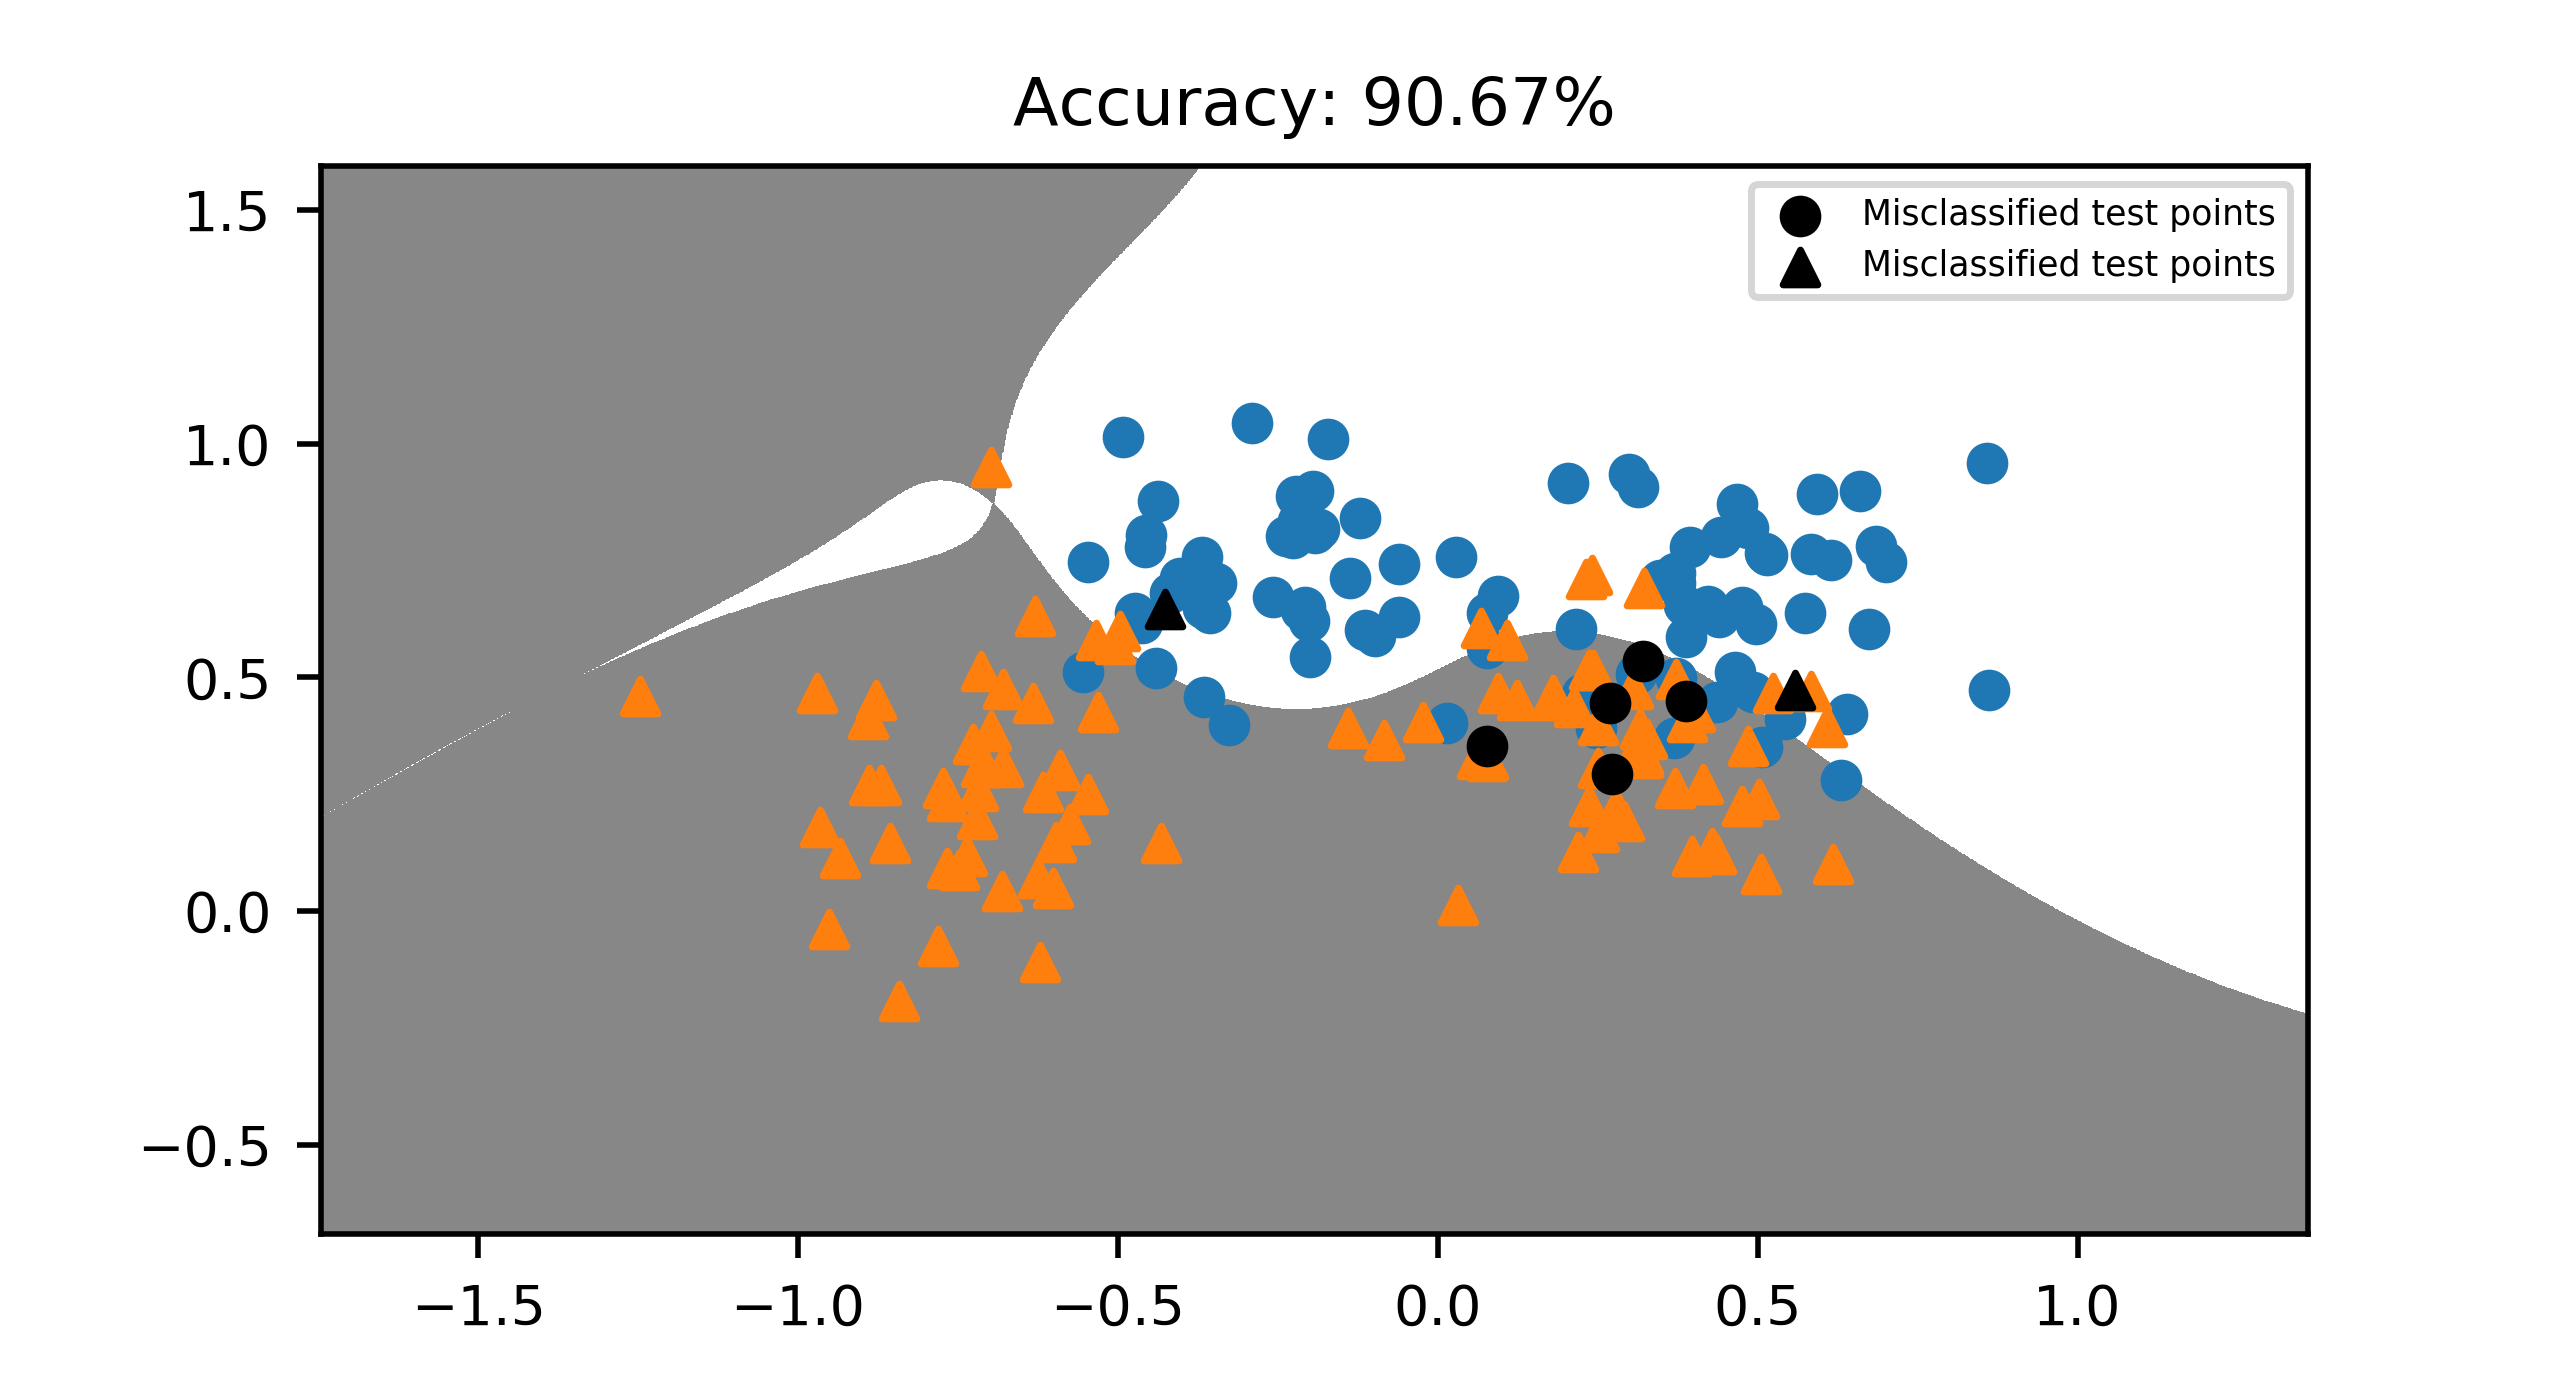
\includegraphics[width=0.5\textwidth]{LSTSVM-Ripley}}
	\subfloat[\lr{KNN-LSTSVM} \lr{($C=2^{-7}, k=6, \gamma=1$)}]{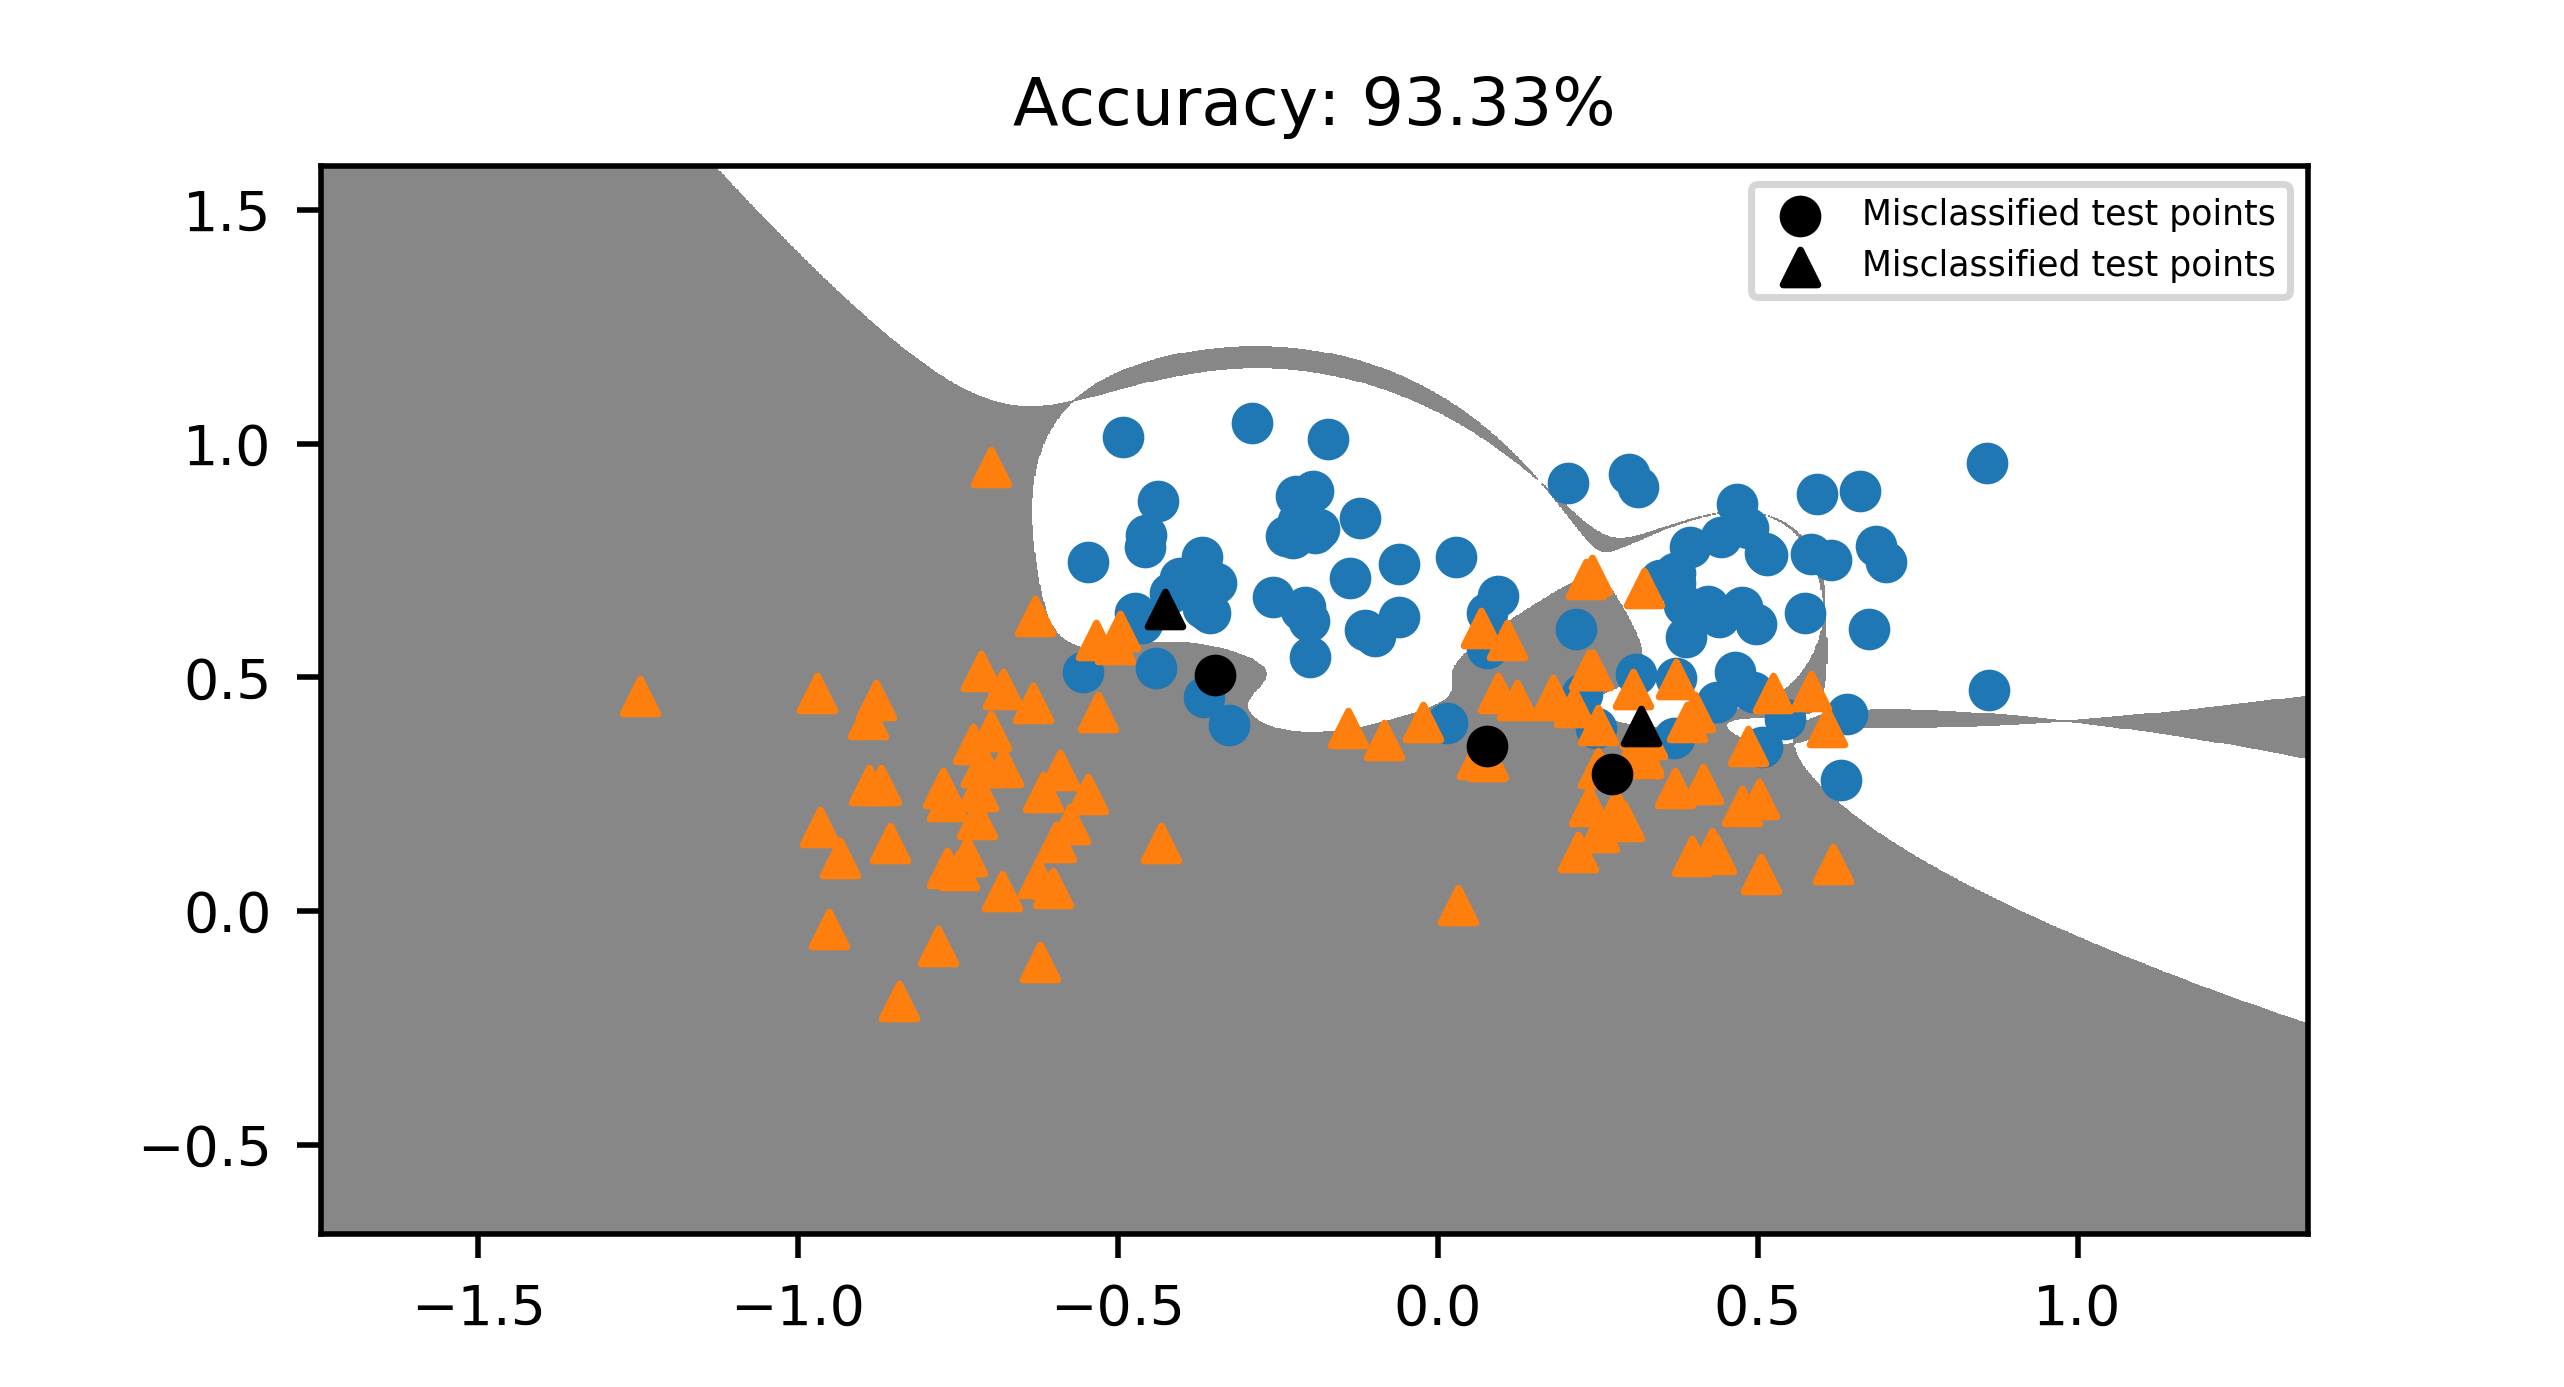
\includegraphics[width=0.5\textwidth]{KNN-LSTSVM-Ripley}}
	\caption{عملکرد و ناحیه تصمیم روش  \lr{LS-TSVM} و  \lr{KNN-LSTSVM} را برای روی داده  \lr{Ripley}}
		\label{fig:LSTSVM-vs-KNN-LSTSVM-R}
\end{figure}

\begin{figure}[!ht]
	\centering
	\subfloat[\lr{LSTSVM} (\lr{$C=2^{-10}, \gamma=2^{1}$})]{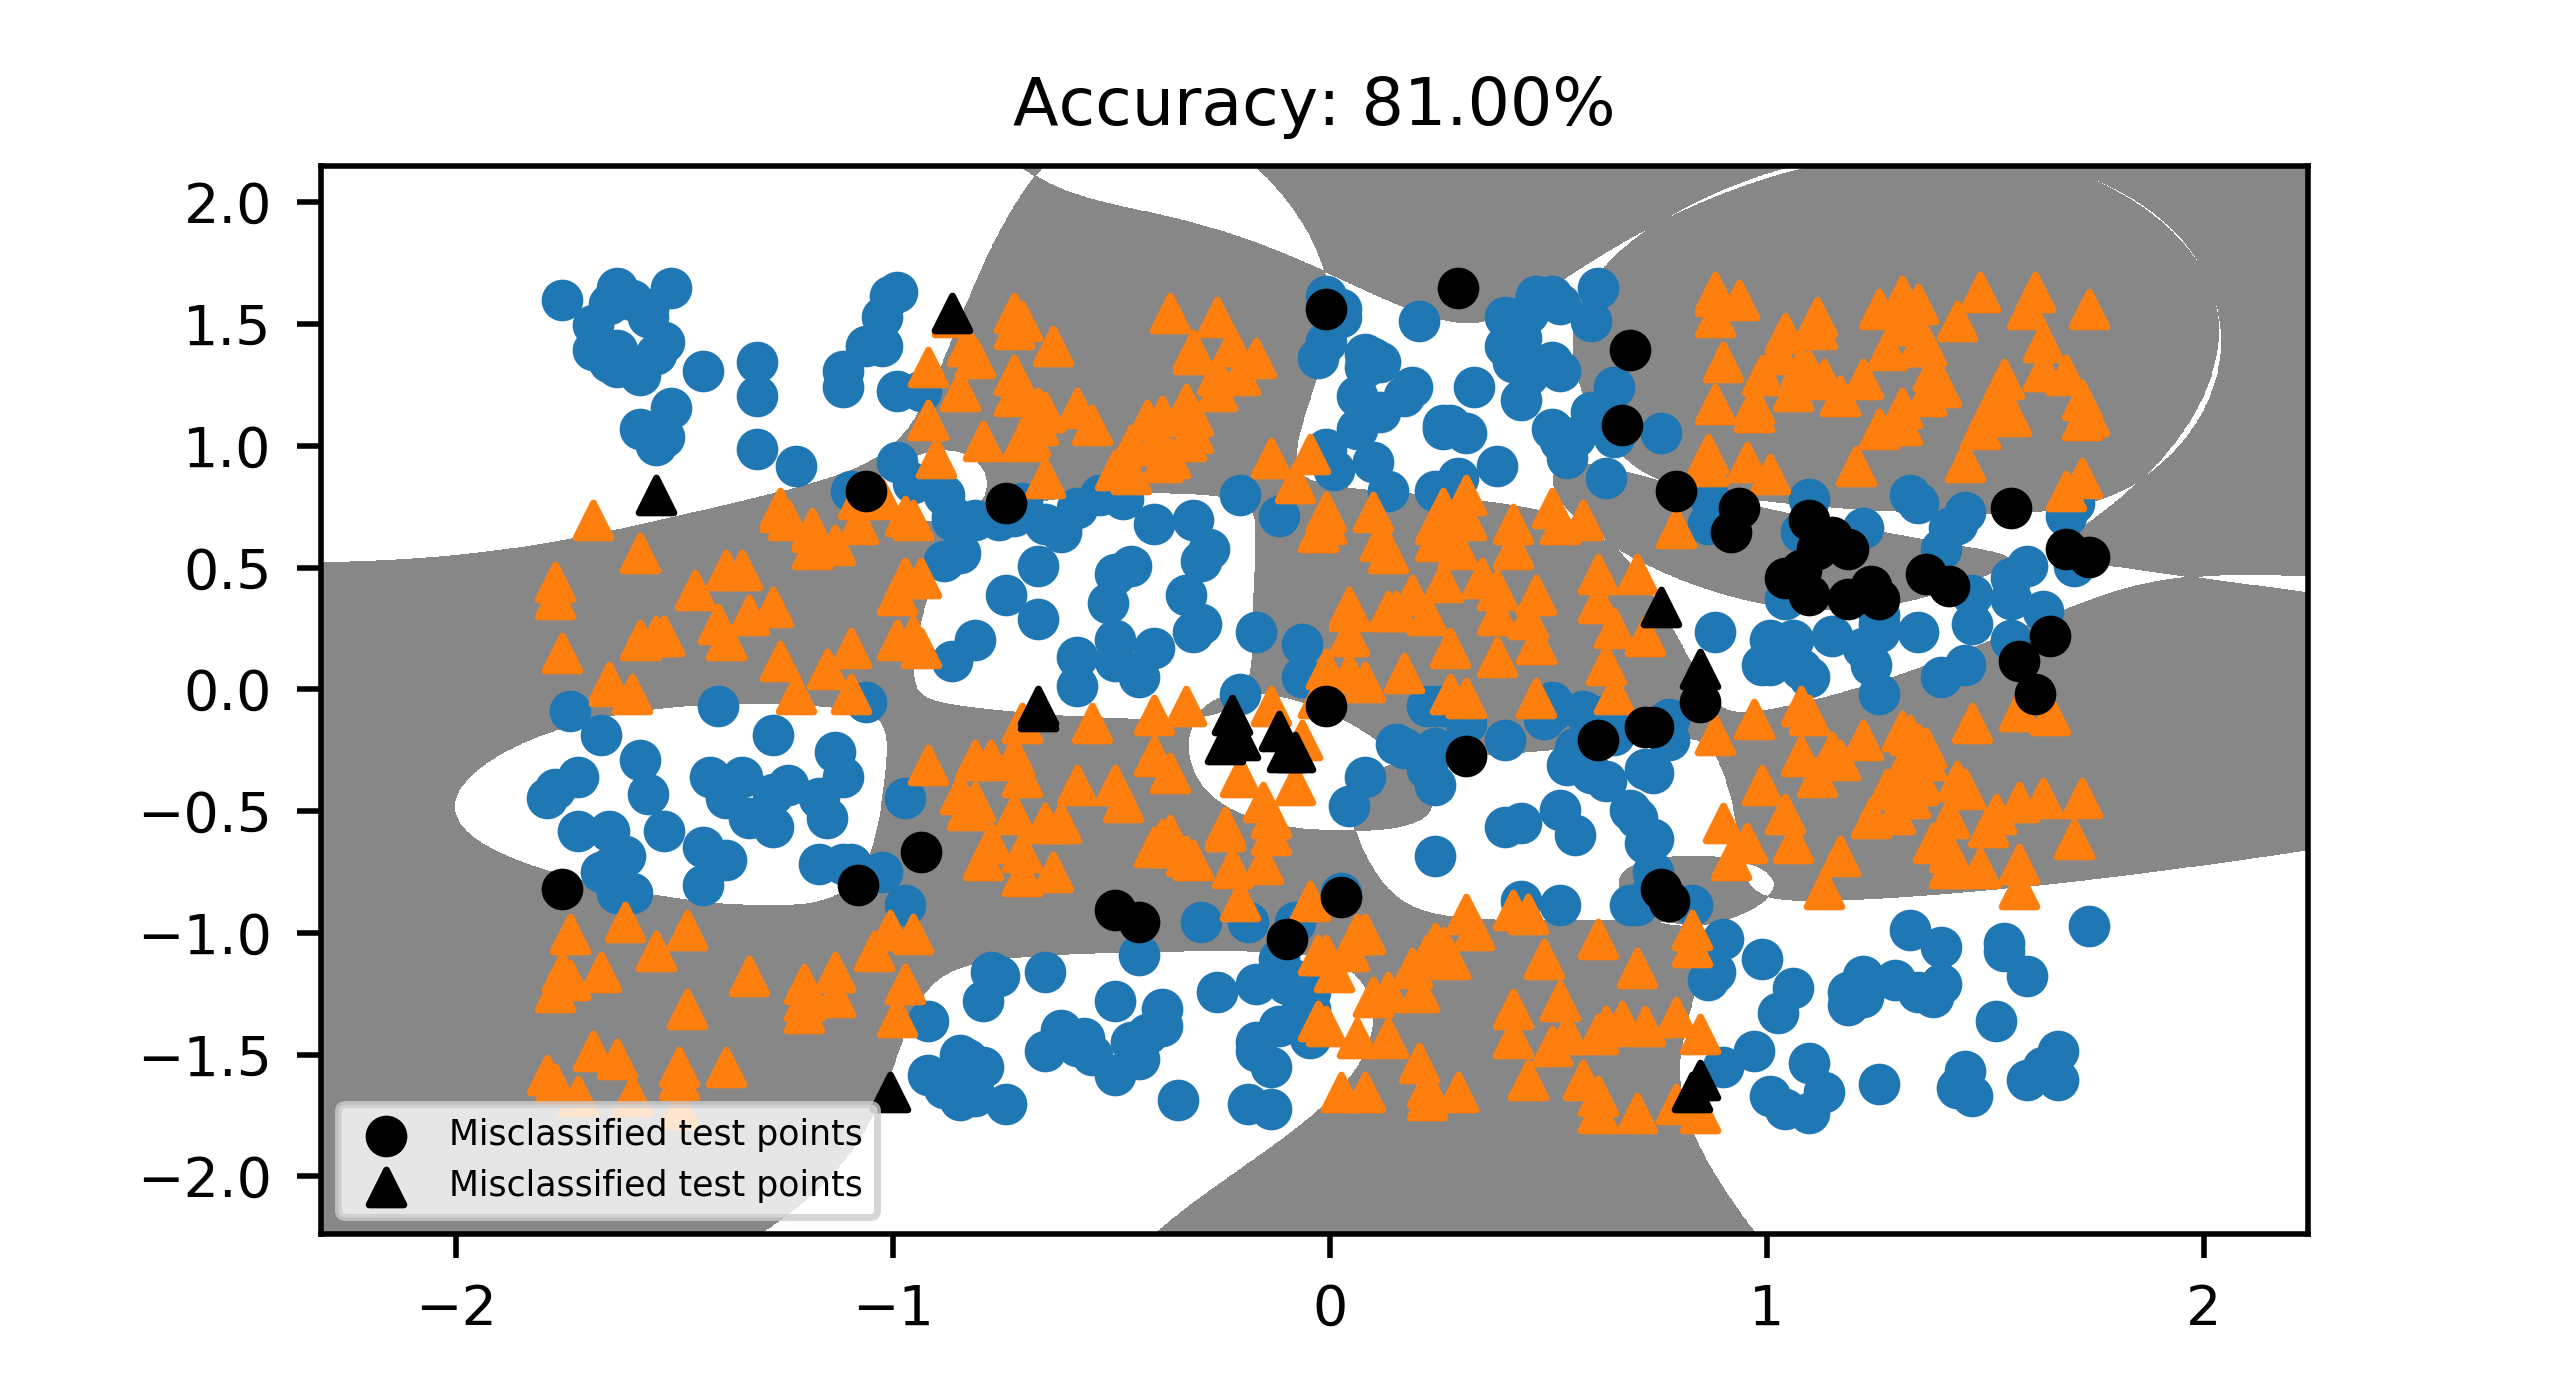
\includegraphics[width=0.5\textwidth]{LSTSVM-check}}
	\subfloat[\lr{KNN-LSTSVM} \lr{($C=2^{-10}, k=6, \gamma=2^{1}$)}]{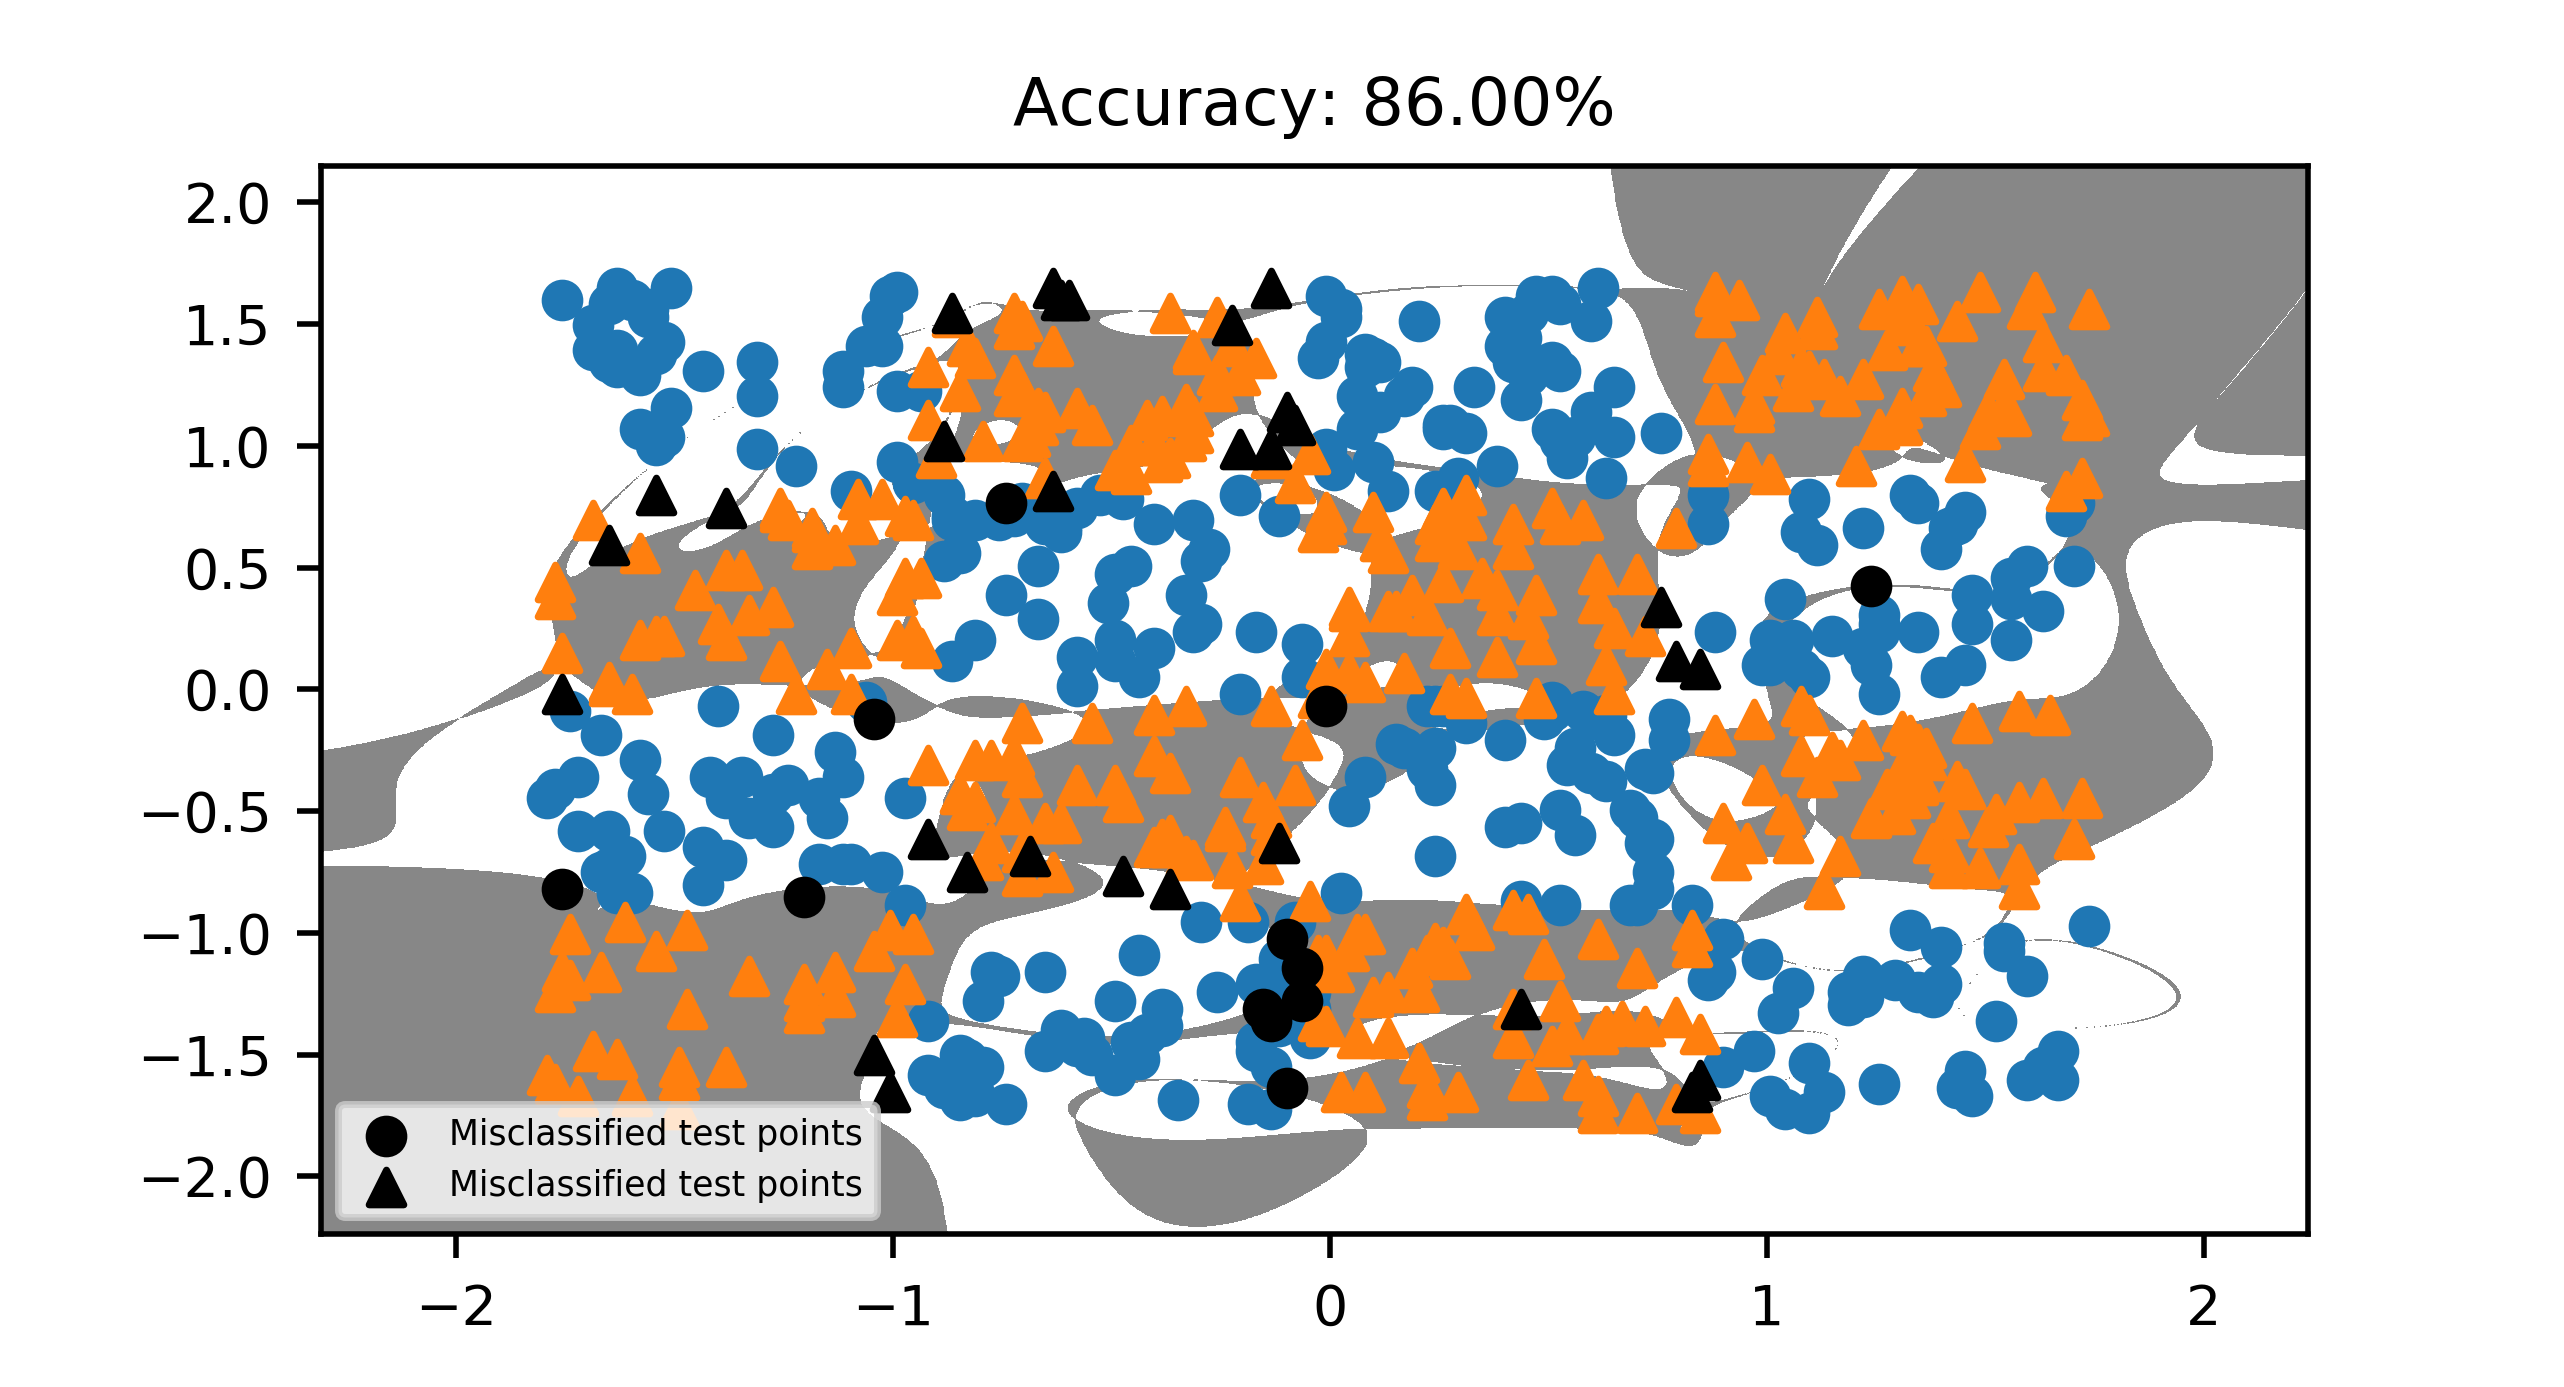
\includegraphics[width=0.5\textwidth]{KNN-LSTSVM-check}}
	\caption{عملکرد و ناحیه تصمیم روش  \lr{LS-TSVM} و  \lr{KNN-LSTSVM} را برای روی داده  \lr{Checkerboard}}
	\label{fig:LSTSVM-vs-KNN-LSTSVM-C}
\end{figure}

\newpage

\subsection{نتایج ارزیابی بر روی مجموعه داده \lr{UCI}}\label{sec:5:2:3}
در این زیر بخش، عملکرد روش \lr{KNN-LSTSVM} روی 14 مجموعه داده از مخرن  \lr{UCI}\LTRfootnote{\lr{https://archive.ics.uci.edu/ml/index.php}} ارزیابی و بررسی می‌شود. مشخصات این مجموعه داده‌ها در جدول \ref{tab:1} ذکر شده است.

\begin{table}[!t]
	\centering
	\caption{مشخصات مجموعه داده‌ها برای ارزیابی روش \lr{KNN-LSTSVM}}
	%\tabcolsep=0.11cm
	\begin{tabular}{l c c c c}
		\hline
		% after \\: \hline or \cline{col1-col2} \cline{col3-col4} ...
		مجموعه داده & تعداد نمونه‌ها & نمونه‌های مثبت & نمونه‌های منفی &تعداد ویژگی‌ها \\
		\hline
	\lr{{Austrailian}} & {690} & {307} & {383} & {14} \\
	\lr{{Bupa-Liver}} & {345} & {145} & {200} & {6} \\
	\lr{{Cleveland}} & {303} & {139} & {164} & {13} \\
	\lr{{Haber-Man}} & {306} & {225} & {81} & {3} \\
	\lr{{Heart-Statlog}} & {270} & {120} & {150} & {13} \\
	\lr{{Hepatits}} & {155} & {32} & {123} & {19} \\
	\lr{{Ionsphere}} & {351} & {225} & {126} & {34} \\
	\lr{{Monk3}} & {554} & {288} & {266} & {6} \\
	\lr{{Pima-Indian}} & {768} & {268} & {500} & {8} \\
	\lr{{Sonar}} & {208} & {97} & {111} & {60} \\
	\lr{{Titanic}} & {891} & {342} & {549} & {7} \\
	\lr{{Votes}} & {435} & {267} & {168} & {16} \\
	\lr{{Wdbc}} & {569} & {212} & {357} & {30} \\
	\lr{{Wpbc}} & {198} & {47} & {151} & {33} \\
		\hline
	\end{tabular}
	
	\label{tab:1}
\end{table}

دقت دسته‌بندی هر کدام از روش‌ها توسط معیار ارزیابی اعتبارسنج ضربدری  ۱۰تایی سنجیده می‌شود. بطوریکه نمونه‌های آموزشی به صورت تصادفی به 10 بخش تقیسم می‌شوند. یکی از این بخش‌ها به عنوان نمونه‌های تست در نظر گرفته می‌شود و سایر بخش‌ها برای آموزش دسته‌بند استفاده می‌گردد. این فرآیند 10 بار تکرار می‌شود تا زمانی که تمام بخش‌ها به عنوان نمونه تست استفاده شود \cite{bishop2006}.

جدول ‏5 2 میانگین و انحراف معیار دقت (به درصد) را برای دسته‌بندهای \lr{TSVM}، \lr{WLTSVM}، \lr{LSTSVM} و \lr{KNN-LSTSVM }نشان می‌دهد. همچنین زمان آموزش دسته‌بندها (به ثانیه) و مقادیر بهینه ‍پارامترها نیز در جدول ‏\ref{tab:3} درج شده است. لازم به ذکر است که محاسبه گراف نزدیک‌ترین همسایه در زمان آموزش دسته‌بندهای \lr{WLTSVM} و \lr{KNN-LSTSVM} لحاظ شده است. 

\begin{table*}[!t]
	\small
	\centering
	\caption{مقایسه دقت و زمان آموزش دسته‌بندهای \lr{TSVM}، \lr{WLTSVM}،  \lr{LSTSVM} و \lr{KNN-LSTSVM}}
	\ra{1.3} % Space between rows
	\tabcolsep=0.13cm % Adjusts column width
	\resizebox{\textwidth}{!}{\begin{tabular}{p{1.95cm} p{1.95cm} p{1.1cm} c p{1.95cm} p{1.1cm} c p{1.95cm} p{1.1cm} c p{1.95cm} p{1.1cm}}
		\toprule
		
		% after \\: \hline or \cline{col1-col2} \cline{col3-col4} ...
		مجموعه داده & \multicolumn{2}{c}{\lr{TSVM}} && \multicolumn{2}{c}{\lr{WLTSVM}} && \multicolumn{2}{c}{\lr{LSTSVM}} && \multicolumn{2}{c}{\lr{KNN-LSTSVM}} \\
		\cmidrule{2-3} \cmidrule{5-6} \cmidrule{8-9} \cmidrule{11-12}
		($m\times n$) & دقت (\%) & زمان اجرا && دقت (\%) & زمان اجرا && دقت (\%) & زمان اجرا &&  دقت (\%) & زمان اجرا \\
		& $(C_1, C_2, \gamma)$  &  && $(C_, \gamma, k)$ &  && $(C_1, C_2, \gamma)$  &  && $(C, \gamma, k)$  &  \\
		\midrule
		\lr{Australian} & \textbf{$87.97\pm2.75$} & $0.070$ && $87.25\pm3.65$ & $0.264$ && $87.68\pm3.79$ & $0.058$ &&  $87.39\pm3.31$ & $0.230$ \\
		($690\times 14$) & ($2^{-4}, 2^{-4}, 2^{-6}$) &  && ($2^{-1}, 2^{-14}, 6$) &  && ($2^{-7}, 2^{-5}, 2^{-6}$) &  && ($2^{3}, 2^{-13}, 7$) &  \\
		\lr{Bupa-Liver} & $73.62\pm4.77$ & $0.082$ && $74.82\pm3.84$ & $0.193$ && $74.51\pm6.89$ & $0.007$ &&  \textbf{$75.96\pm5.40$} & $0.041$ \\
		($345\times 6$) & ($2^{-3}, 2^{-3}, 2^{-6}$) &  && ($2^{2}, 2^{-7}, 4$) &  && ($2^{5}, 2^{4}, 2^{-6}$) &  && ($2^{10}, 2^{-6}, 7$) &  \\
		\lr{Cleveland} & $84.86\pm3.76$ & $0.037$ && $84.48\pm6.29$ & $0.082$ && $85.49\pm4.92$ & $0.005$ &&  \textbf{$85.51\pm6.41$} & $0.026$ \\
		($303\times 13$) & ($2^{0}, 2^{-1}, 2^{-11}$) &  && ($2^{3}, 2^{-9}, 7$) &  && ($2^{2}, 2^{1}, 2^{-11}$) &  && ($2^{-2}, 2^{-15}, 5$) &  \\
		\lr{Haber-Man} & $76.14\pm3.60$ & $0.082$ && $75.80\pm5.22$ & $0.138$ && $76.73\pm7.83$ & $0.005$ &&  \textbf{$76.81\pm5.82$} & $0.031$ \\
		($306\times 3$) & ($2^{1}, 2^{-1}, 2^{-9}$) &  && ($2^{3}, 2^{-4}, 2$) &  && ($2^{9}, 2^{9}, 2^{-7}$) &  && ($2^{-10}, 2^{-9}, 9$) &  \\
		\lr{Heart-Statlog} & \textbf{$85.56\pm5.84$} & $0.041$ && $85.19\pm5.49$ & $0.032$ && $85.19\pm6.20$ & $0.004$ &&  $85.19\pm5.74$ & $0.022$ \\
		($270\times 13$) & ($2^{1}, 2^{0}, 2^{-11}$) &  && ($2^{1}, 2^{-13}, 6$) &  && ($2^{0}, 2^{-1}, 2^{-12}$) &  && ($2^{-1}, 2^{-14}, 7$) &  \\
		\lr{Hepatits} & $85.79\pm8.65$ & $0.003$ && $86.50\pm8.79$ & $0.040$ && \textbf{$87.79\pm6.57$} & $0.001$ &&  $87.13\pm7.59$ & $0.006$ \\
		($155\times 19$) & ($2^{-4}, 2^{-2}, 2^{-8}$) &  && ($2^{8}, 2^{-3}, 3$) &  && ($2^{3}, 2^{5}, 2^{-11}$) &  && ($2^{-1}, 2^{-5}, 7$) &  \\
		\lr{Ionsphere} & \textbf{$92.59\pm3.19$} & $0.028$ && $92.04\pm5.50$ & $0.126$ && $91.74\pm4.32$ & $0.006$ &&  \textbf{$92.59\pm4.47$} & $0.040$ \\
		($351\times 34$) & ($2^{-1}, 2^{-3}, 2^{-5}$) &  && ($2^{1}, 2^{1}, 3$) &  && ($2^{6}, 2^{1}, 2^{-5}$) &  && ($2^{1}, 2^{-5}, 5$) &  \\
		\lr{Monk3} & $98.37\pm1.26$ & $0.150$ && $98.38\pm1.69$ & $0.494$ && $98.55\pm1.36$ & $0.032$ &&  \textbf{$98.56\pm1.34$} & $0.126$ \\
		($554\times 6$) & ($2^{-4}, 2^{2}, 2^{-3}$) &  && ($2^{3}, 2^{-6}, 2$) &  && ($2^{-6}, 2^{-3}, 2^{-3}$) &  && ($2^{0}, 2^{-3}, 5$) &  \\
		\lr{Pima-Indian} & $77.87\pm4.73$ & $0.147$ && $77.86\pm3.49$ & $0.566$ && $77.61\pm5.89$ & $0.073$ &&  \textbf{$78.01\pm3.64$} & $0.339$ \\
		($768\times 8$) & ($2^{1}, 2^{1}, 2^{-3}$) &  && ($2^{4}, 2^{-5}, 2$) &  && ($2^{-1}, 2^{-1}, 2^{-4}$) &  && ($2^{-1}, 2^{-4}, 10$) &  \\
		\lr{Sonar} & $86.14\pm8.35$ & $0.012$ && \textbf{$87.50\pm3.17$} & $0.033$ && $85.55\pm8.31$ & $0.002$ &&  $87.48\pm6.65$ & $0.011$ \\
		($208\times 60$) & ($2^{-5}, 2^{-1}, 2^{-3}$) &  && ($2^{5}, 2^{-4}, 7$) &  && ($2^{-10}, 2^{3}, 2^{-3}$) &  && ($2^{-4}, 2^{-6}, 4$) &  \\
		\lr{Titanic} & $81.94\pm3.23$ & $0.225$ && $81.49\pm4.70$ & $0.692$ && \textbf{$82.38\pm4.63$} & $0.108$ &&  $82.27\pm3.80$ & $0.486$ \\
		($891\times 7$) & ($2^{-4}, 2^{-5}, 2^{-3}$) &  && ($2^{0}, 2^{-6}, 7$) &  && ($2^{1}, 2^{1}, 2^{-5}$) &  && ($2^{8}, 2^{-5}, 10$) &  \\
		\lr{Votes} & $96.78\pm2.11$ & $0.145$ && $97.01\pm1.79$ & $0.098$ && \textbf{$97.02\pm2.89$} & $0.012$ &&  $97.01\pm3.11$ & $0.064$ \\
		($435\times 16$) & ($2^{-6}, 2^{-3}, 2^{-6}$) &  && ($2^{7}, 2^{-13}, 7$) &  && ($2^{-6}, 2^{-3}, 2^{-9}$) &  && ($2^{6}, 2^{-9}, 3$) &  \\
		\lr{Wdbc} & \textbf{$98.42\pm1.23$} & $0.003$ && $97.54\pm2.51$ & $0.206$ && $98.07\pm2.54$ & $0.034$ &&  $97.72\pm1.12$ & $0.154$ \\
		($569\times 30$) & ($2^{-3}, 2^{-1}, 2^{-8}$) &  && ($2^{-2}, 2^{-5}, 6$) &  && ($2^{-4}, 2^{-2}, 2^{-8}$) &  && ($2^{-5}, 2^{-7}, 5$) &  \\
		\lr{Wpbc} & $82.39\pm9.20$ & $0.006$ && $80.84\pm8.94$ & $0.019$ && $81.32\pm9.01$ & $0.002$ &&  \textbf{$82.76\pm5.48$} & $0.010$ \\
		($198\times 33$) & ($2^{-4}, 2^{-5}, 2^{-6}$) &  && ($2^{1}, 2^{-10}, 2$) &  && ($2^{-2}, 2^{-4}, 2^{-7}$) &  && ($2^{-2}, 2^{-7}, 6$) &  \\
		\midrule
		میانگین دقت  & \multicolumn{2}{c}{$86.31$} && \multicolumn{2}{c}{$86.19$} && \multicolumn{2}{c}{$86.40$} && \multicolumn{2}{c}{\textbf{$86.74$}} \\
		\bottomrule
	\end{tabular}}
	
	\label{tab:3}
\end{table*}

نتایج بدست آمده به این صورت تحلیل و بررسی می‌شود:
\begin{enumerate}
	\item از نظر دقت دسته‌بندی، روش پیشنهادی (\lr{KNN-LSTSVM}) از سه روش دیگر بهتر عمل کرده است. زیرا روش \lr{KNN-LSTSVM} با استفاده از گراف نزدیک‌ترین همسایه، اطلاعات شباهت نمونه‌ها را در تابع هدف لحاظ می‌کند. از این رو ابرصفحه غیر موازی در روش پیشنهادی به نمونه‌های پرتراکم نزدیک‌تر و از نمونه‌های حاشیه‌ای حداکثر فاصله را می‌گیرد. در حالی که روش‌های \lr{TSVM} و \lr{LSTSVM}  نمونه‌های حاشیه‌ای را در نظر نمی‌گیرد.
	\item از نظر زمان آموزش و پیچیدگی محاسباتی، روش \lr{LSTSVM} از سایر روشها سریع‌تر است. زیرا در این روش فقط دو دستگاه معادلات خطی حل می‌گردد. با این حال روش پیشنهادی (\lr{KNN-LSTSVM}) از روش \lr{WLTSVM} و \lr{TSVM} به طور قابل توجه‌ای سریع‌تر است. زیرا روش پیشنهادی دو دستگاه معادلات خطی حل می‌کند، در حالی‌که روش \lr{WLTSVM} و \lr{TSVM} دو مسئله دوگان درجه دو را حل می‌کنند.
	\item به منظور بررسی اثر پارامتر  $k$ روی دقت روش \lr{KNN-LSTSVM}، آزمایش روی مجموعه داده‌های \lr{Australian} و \lr{Hepatitis} صورت گرفته است. مقادیر پارامتر  $k$ بین 2 تا 30 با گام 2 تعیین شده است. شکل ‏ \ref{fig:KNN-LSTSVM-Aust-Hepa} اهمیت انتخاب پارامتر   را نشان می‌دهد. بیشترین دقت برای مجموعه داده \lr{Australian} با پارامتر  $k=12$ بدست آمده است. به عبارت دیگر،  پارامتر بهینه برای مجموعه داده \lr{Australian} می‌باشد. از طرف دیگر، افزایش مقدار  $k$ برای مجموعه داده \lr{Hepatitis} باعث بهبود دقت روش \lr{KNN-LSTSVM} می‌شود. به طور کلی، انتخاب بهینه پارامتر  $k$ روی عملکرد روش پیشنهادی تاثیر زیادی دارد.
\end{enumerate}

\begin{figure}[!t]
	\centering
	\subfloat[مجموعه داده \lr{Australian}]{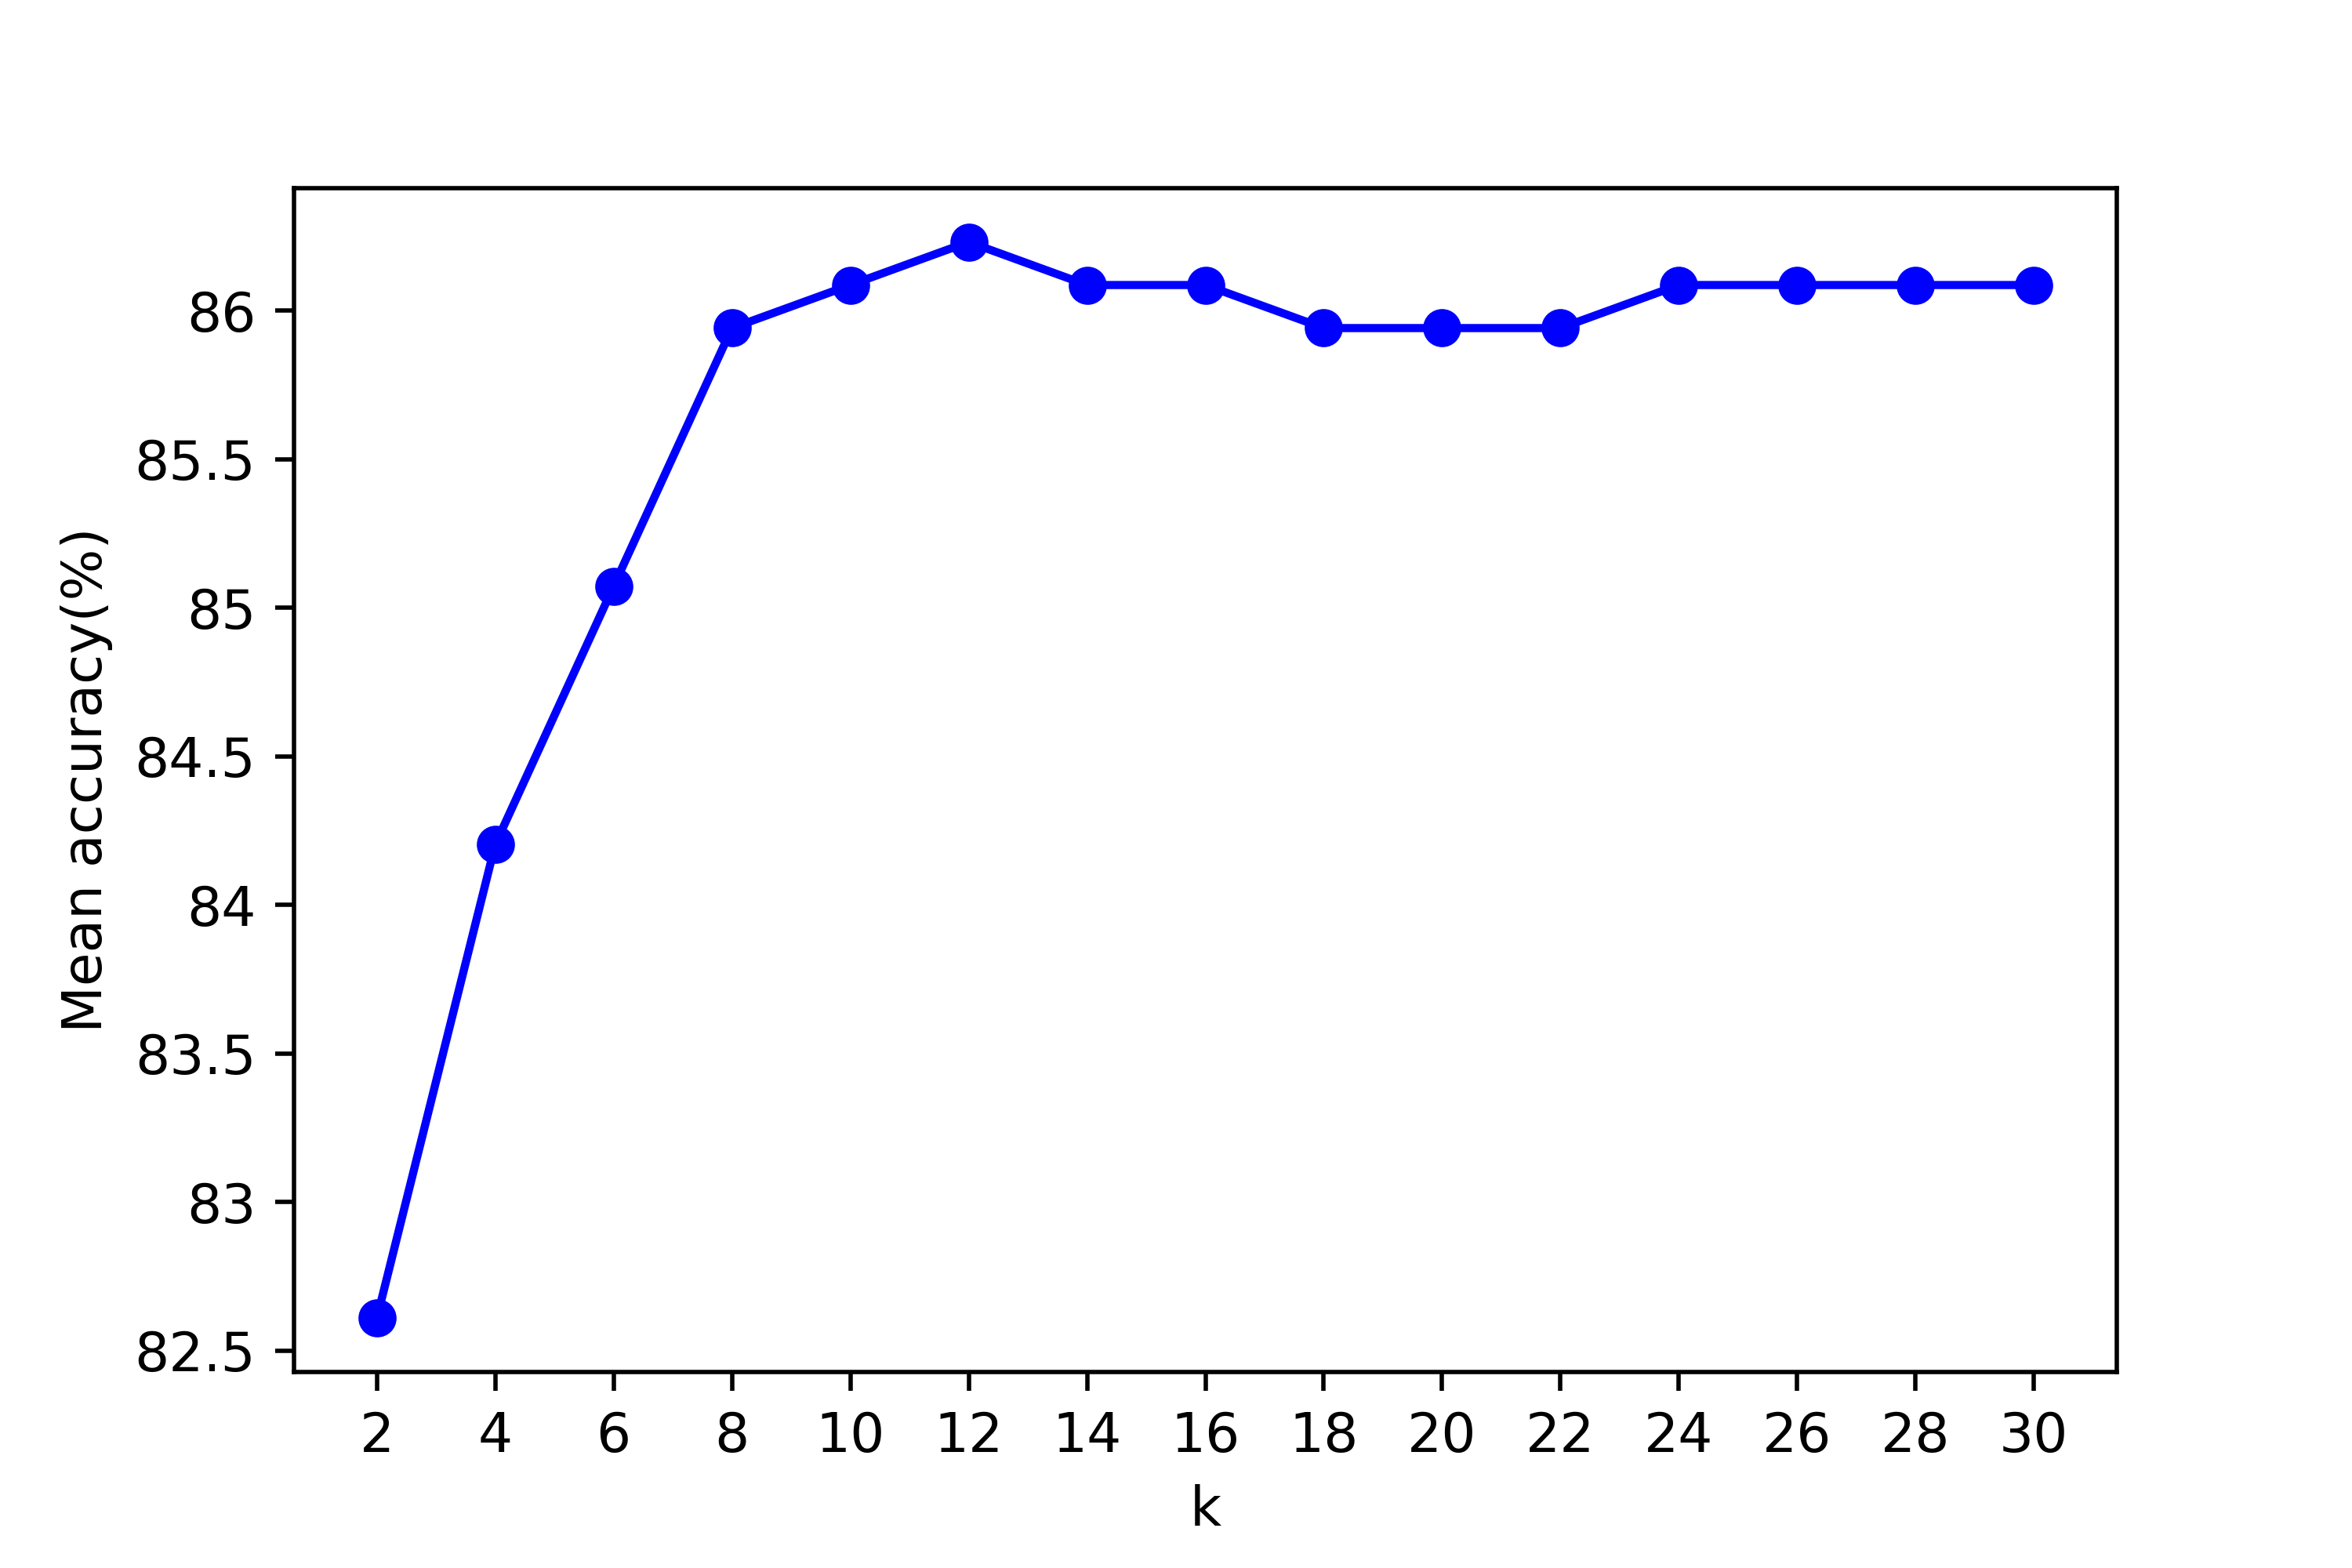
\includegraphics[width=0.5\textwidth]{KNN-LSTSVM-Aust}}
	\subfloat[مجموعه داده \lr{Hepatitis}]{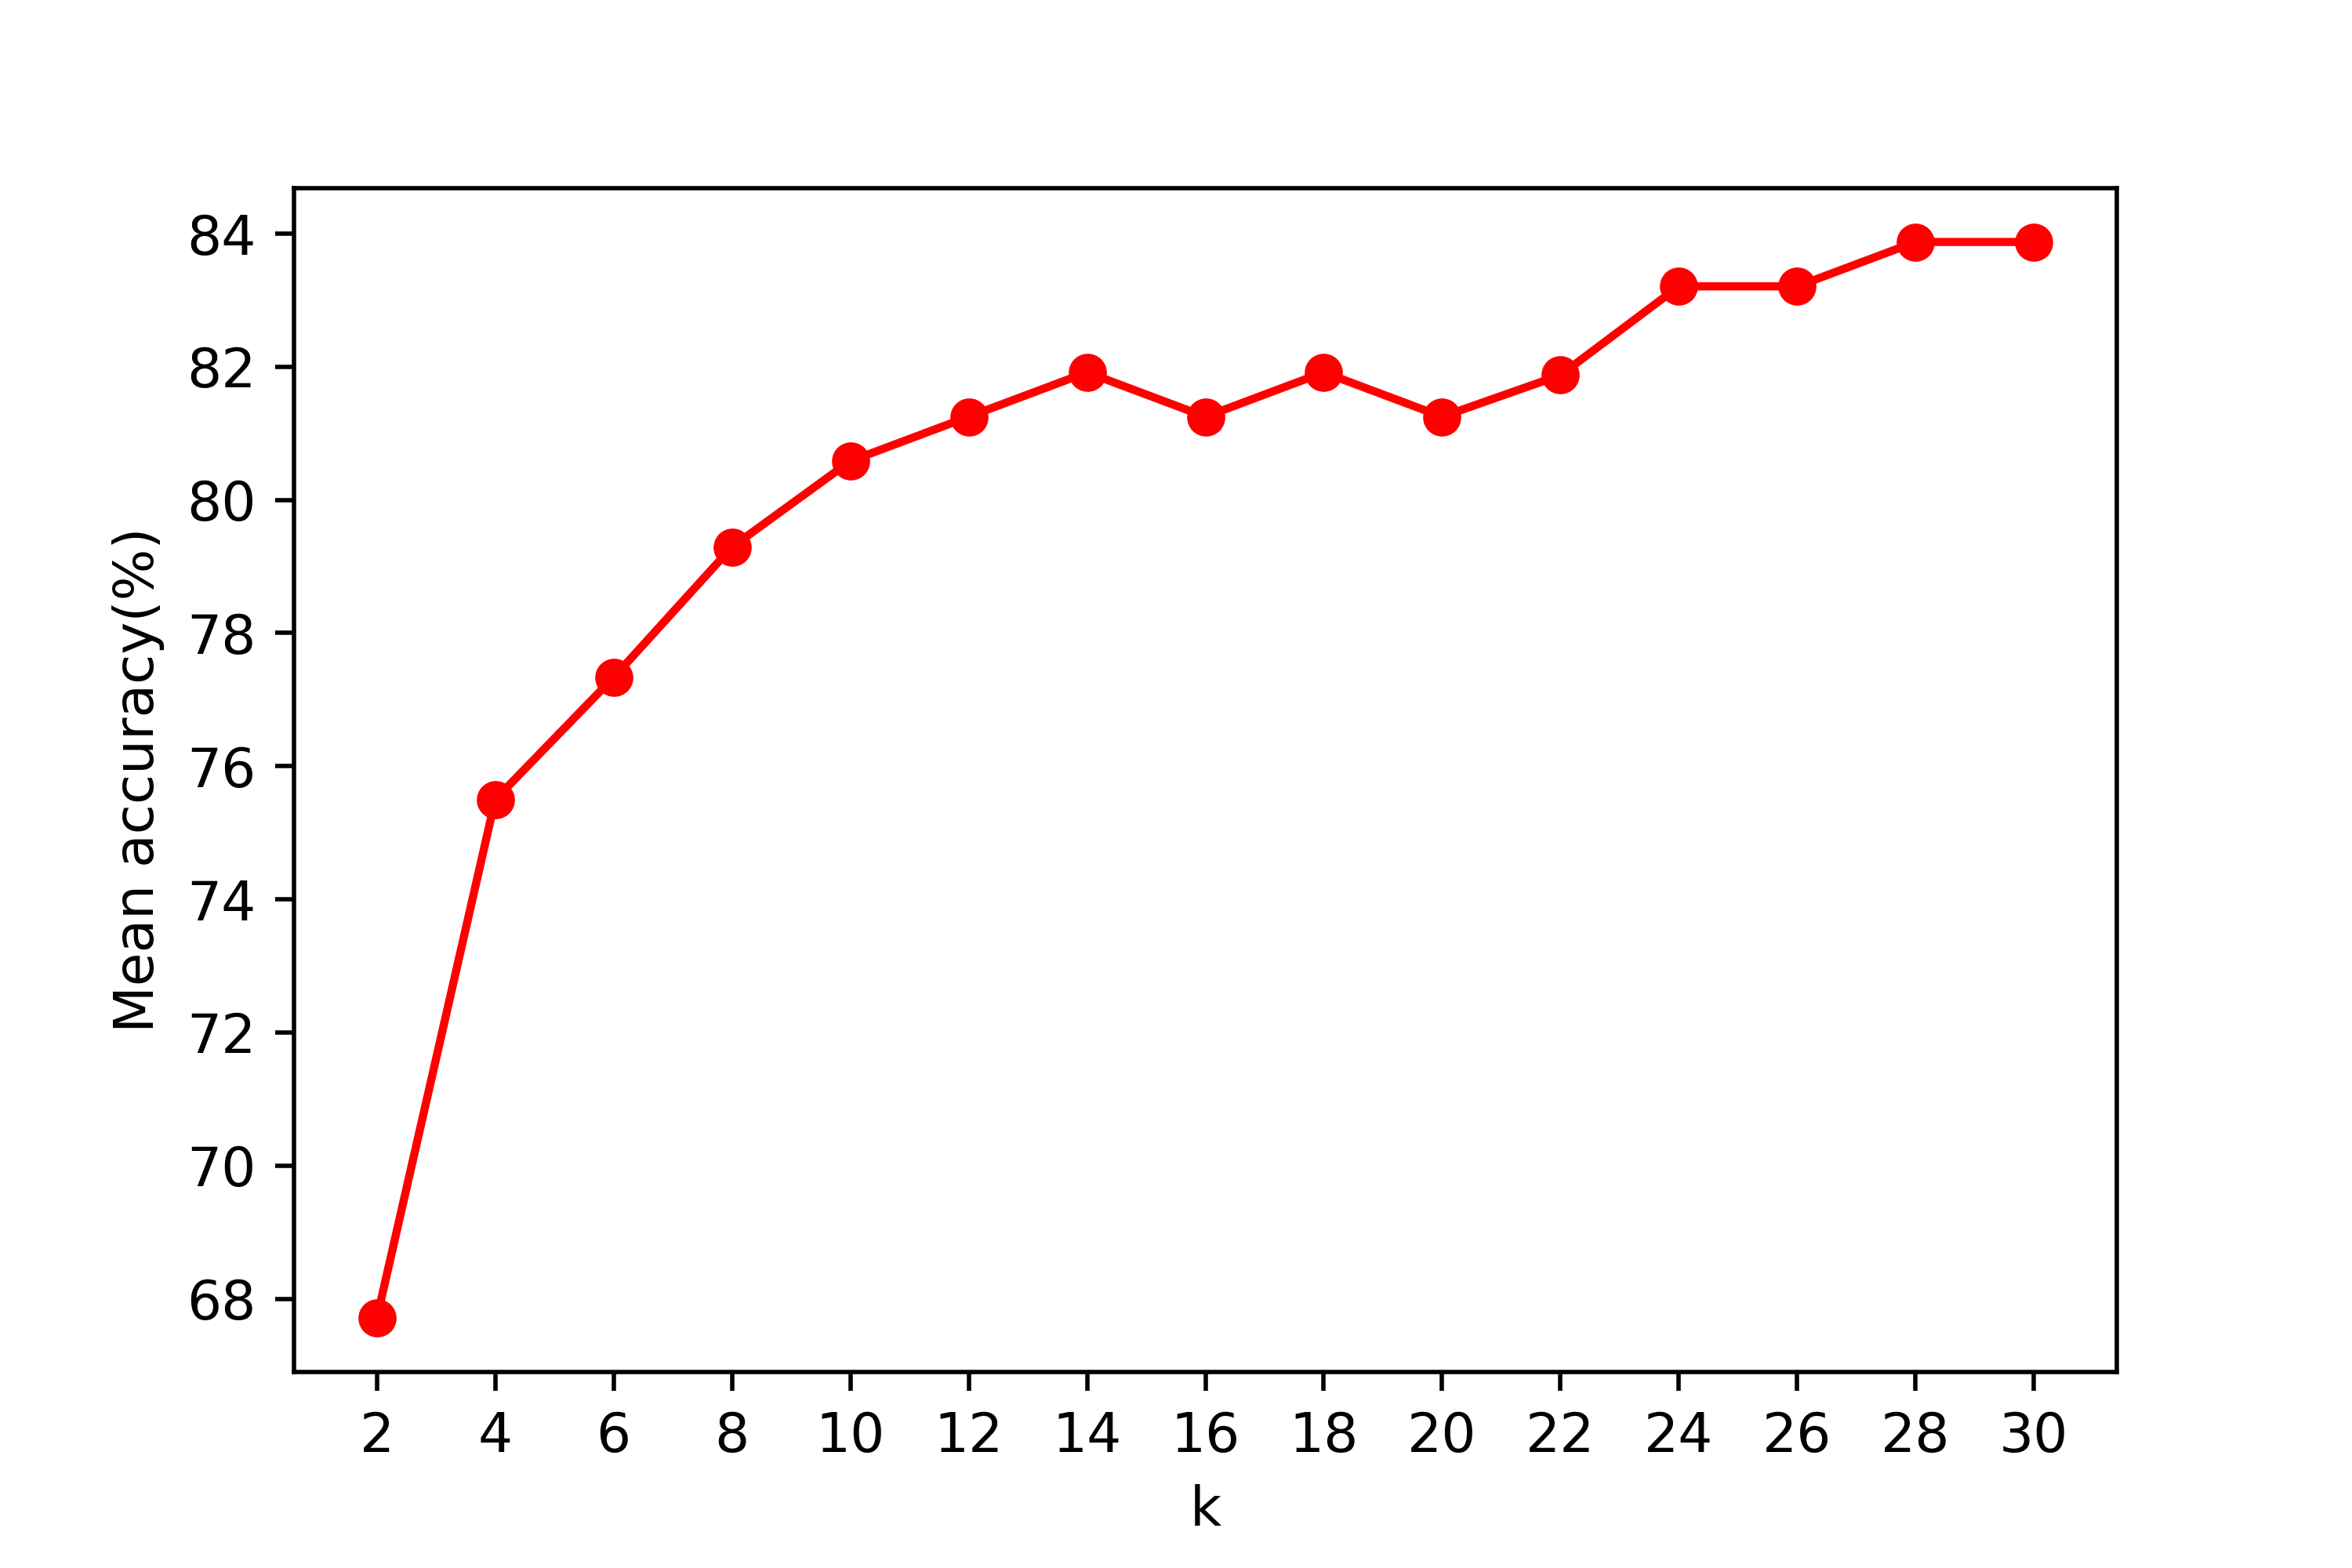
\includegraphics[width=0.5\textwidth]{KNN-LSTSVM-Hepa}}
	\caption{اثر افزایش پارامتر $k$ روی دقت دسته‌بند \lr{KNN-LSTSVM}}
	\label{fig:KNN-LSTSVM-Aust-Hepa}
\end{figure}

\subsubsection{بررسی آماری}\label{sec:5:2:3:1}
به منظور تحلیل بیشتر عملکرد چهار روش روی 14 مجموعه داده (\ref{tab:3})، آزمون‌های آماری طبق پیشنهاد دمسار\LTRfootnote{\lr{Demsar}} \cite{demsar2006} استفاده می‌شود. بدین منظور آزمون آماری ساده و ناپارامتریک فریدمن\LTRfootnote{\lr{Friedman}}  مورد استفاده قرار گرفته است. به منظور انجام آزمون آماری، میانگین رتبه چهار روش بر اساس دقت محاسبه شده و در جدول ‏\ref{tab:4} نشان داده شده است. ابتدا بر اساس فرض صفر، تمام روش‌ها را یکسان در نظر می‌گیریم. سپس آزمون فریدمن با رابطه زیر محاسبه می‌شود.
\begin{equation}\label{eq:5:1}
\chi^2_F = \frac{12N}{k(k + 1)}\bigg[\sum_{j} R^2_j - \frac{k(k + 1)^2}{4} \bigg],
\end{equation}

در رابطه \ref{eq:5:1}،  $R_j=\frac{1}{N}\sum_{i}r^j_i$ و $r_{i}^{j}$  نشان‌دهنده رتبه $j$مین روش بر روی $i$مین مجموعه داده از  $N$ است. 

\begin{table}[!t]
	\centering
	\caption{میانگین رتبه براساس دقت (ارزیابی \lr{KNN-LSTSVM})}
	\ra{1.3} % Space between rows
	\tabcolsep=0.10cm
	\begin{tabular}{c c c c c c c c c c c c}
		\toprule
		% after \\: \hline or \cline{col1-col2} \cline{col3-col4} ...
		مجموعه داده & \lr{TSVM} & \lr{WLTSVM} & \lr{LSTSVM} & \lr{KNN-LSTSVM} \\
		\midrule
	\lr{Austrailian} & 1 & 4 & 2 & 3\\
	\lr{Bupa-Liver} & 4 & 2 & 3 & 1\\
	\lr{Cleveland} & 3 & 4 & 2 & 1\\
	\lr{Haber-Man} & 3 & 4 & 2 & 1\\
	\lr{Heart-Statlog} & 1 & 3 & 3 & 3\\
	\lr{Hepatits} & 4 & 3 & 1 & 2\\
	\lr{Ionsphere} & $1.5$ & 3 & 4 & $1.5$\\
	\lr{Monk3} & 4 & 3 & 2 & 1\\
	\lr{Pima-Indian} & 2 & 3 & 4 & 1\\
	\lr{Sonar} & 3 & 1 & 4 & 2\\
	\lr{Titanic} & 3 & 4 & 1 & 2\\
	\lr{Votes} & 4 & $2.5$ & 1 & $2.5$\\
	\lr{Wdbc} & 1 & 4 & 2 & 3\\
	\lr{Wpbc} & 2 & 4 & 3 & 1\\
	میانگین رتبه & $2.61$ & $3.18$ & $2.43$ & \textbf{$1.79$} \\
		\bottomrule
	\end{tabular}
	
	\label{tab:4}
\end{table}

سپس مقدار $F_F$  براساس  $\chi^2_F$ به صورت زیر محاسبه می‌شود. بطوریکه $F_F$ از توزیع $F$ با $(k-1)$ و $(k-1)(N-1)$ درجه آزادی پیروی می‌کند.
\begin{equation}\label{eq:5:2}
F_F = \frac{(N - 1)\chi^2_F}{N(k - 1) - \chi^2_F}
\end{equation}

بر اساس روابط \ref{eq:5:1} و \ref{eq:5:2}، مقادیر $\chi^2_F = 8.293$ و  $F_F = 3.198$ بدست آمده است. در اینجا $F_F$ از توزیع $F$  با (39، 3) درجه آزادی پیروی می‌کند. مقادیر ویژه $F(3, 39)$ برای سطوح معناداری 25/0، 1/0 و 05/0 به ترتیب برابر  42/1، 23/2 و 84/2 است. مقدار  $F_F$ به طور قابل توجه‌ای بیشتر از مقدار ویژه است. بنابراین از آزمون آماری استنتاج می‌شود که تفاوت قابل توجه‌ای بین 4 روش وجود دارد. همچنین جدول ‏\ref{tab:6} نشان می‌دهد که روش پیشنهادی (\lr{KNN-LSTSVM}) در مجموع عملکرد بهتری نسبت به سایر روش‌ها دارد. زیرا میانگین رتبه روش پیشنهادی در میان سایر روش‌ها کمترین است.

\subsection{مجموعه داده \lr{NDC}}\label{sec:5:2:4}
به منظور بررسی سرعت آموزش روش پیشنهادی (\lr{RKNN-TSVM}) و مقایسه آن با سایر روش‌ها، آزمایش بر روی مجموعه داده‌های بزرگ صورت گرفته است. مجموعه داده \lr{NDC} \cite{musicant1998} برای این منظور انتخاب شده است. جدول ‏\ref{tab:5} مشخصات این مجموعه داده را نشان می‌دهد.

\begin{table}[!t]
	\centering
	\caption{مشخصات مجموعه داده \lr{NDC}}
	\begin{tabular}{l c c c}
		\toprule
		% after \\: \hline or \cline{col1-col2} \cline{col3-col4} ...
		مجموعه داده & تعداد نمونه‌های آموزش & تعداد نمونه‌های تست & تعداد ویژگی‌ها\\
		\midrule
\lr{{NDC-500}} & {500} & {50} & {32} \\
\lr{{NDC-700}} & {700} & {70} & {32} \\
\lr{{NDC-900}} & {900} & {90} & {32} \\
\lr{{NDC-1K}} & {1000} & {100} & {32} \\
\lr{{NDC-2K}} & {2000} & {200} & {32} \\
\lr{{NDC-3K}} & {3000} & {300} & {32} \\
\lr{{NDC-4K}} & {4000} & {400} & {32} \\
\lr{{NDC-5K}} & {5000} & {500} & {32} \\
\lr{{NDC-10K}} & {10000} & {1000} & {32} \\
\lr{{NDC-25K}} & {25000} & {2500} & {32} \\
\lr{{NDC-50K}} & {50000} & {5000} & {32} \\
		\bottomrule
	\end{tabular}
	
	\label{tab:5}
\end{table}

جهت آزمایش با مجموعه داده \lr{NDC}، پارامتر $C$ برای تمام روش برابر با یک است. در نسخه غیر خطی از تابع \lr{RBF} با پارامتر $\gamma=2^{-15}$ استفاده شده است. همچنین پارامتر  $k$ برای روش‌های \lr{WLTSVM} و \lr{KNN-LSTSVM} برابر با 5 است. جدول \ref{tab:6} زمان آموزش چهار روش بر روی مجموعه داده \lr{NDC} با تابع هسته خطی و \lr{RBF} را نشان می‌دهد.

\begin{sidewaystable*}
%\begin{table*}[!t]
	\centering
	\caption{مقایسه زمان آموزش روش \lr{KNN-LSTSVM} و سایر روش‌ها بر روی مجموعه داده \lr{NDC}}
	\ra{1.3} % Space between rows
	\begin{threeparttable}
		\begin{tabular}{c c c c c c c c c c c c c}
			\toprule
			% after \\: \hline or \cline{col1-col2} \cline{col3-col4} ...
			&& \multicolumn{2}{c}{\lr{TSVM}} && \multicolumn{2}{c}{\lr{WLTSVM}} && \multicolumn{2}{c}{\lr{LSTSVM}} && \multicolumn{2}{c}{\lr{KNN-LSTSVM}} \\
			مجموعه داده && \multicolumn{2}{c}{زمان اجرا} && \multicolumn{2}{c}{زمان اجرا} && \multicolumn{2}{c}{زمان اجرا} && \multicolumn{2}{c}{زمان اجرا} \\
			\cmidrule{3-4} \cmidrule{6-7} \cmidrule{9-10} \cmidrule{12-13}
		&تابع هسته	& خطی & \lr{RBF} && خطی & \lr{RBF} && خطی & \lr{RBF} && خطی & \lr{RBF} \\
			\midrule
			\lr{NDC-500} && $0.222$ & $0.324$ && $0.583$ & $0.838$ && $0.004$ & $0.034$ && $0.031$ & $0.399$ \\
			\lr{NDC-700} && $0.45$ & $0.744$ && $1.115$ & $1.741$ && $0.004$ & $0.064$ && $0.053$ & $0.757$ \\
			\lr{NDC-900} && $0.83$ & $1.111$ && $1.884$ & $2.761$ && $0.004$ & $0.223$ && $0.084$ & $1.362$ \\
			\lr{NDC-1K} && $0.976$ & $1.599$ && $2.315$ & $3.499$ && $0.004$ & $0.266$ && $0.1$ & $1.657$ \\
			\lr{NDC-2K} && $6.606$ & $12.746$ && $16.297$ & $22.474$ && $0.004$ & $1.055$ && $0.387$ & $6.21$ \\
			\lr{NDC-3K} && $25.387$ & $41.908$ && $73.451$ & $70.213$ && $0.004$ & $2.588$ && $0.904$ & $14.041$ \\
			\lr{NDC-4K} && $72.19$ & $129.932$ && $163.249$ & $176.899$ && $0.005$ & $5.314$ && $1.647$ & $25.812$ \\
			\lr{NDC-5K}\lr{\textsuperscript{b}} && $137.909$ & $277.463$ && $319.574$ & $339.347$ && $0.005$ & $10.024$ && $2.618$ & $39.788$ \\
			\lr{NDC-10K}\lr{\textsuperscript{b}} && $696.562$ & \lr{\tnote{a}} && \lr{\tnote{a}} & \lr{\tnote{a}} && $0.007$ & $67.475$ && $11.249$ & $164.655$ \\
			\lr{NDC-25K}\lr{\textsuperscript{b}} && \lr{\tnote{a}} & \lr{\tnote{a}} && \lr{\tnote{a}} & \lr{\tnote{a}} && $0.011$ & $967.458$ && $75.707$ & \lr{\tnote{a}} \\
			\lr{NDC-50K}\lr{\textsuperscript{b}} && \lr{\tnote{a}} & \lr{\tnote{a}} && \lr{\tnote{a}} & \lr{\tnote{a}} && $0.02$ & \lr{\tnote{a}} && $383.829$ & \lr{\tnote{a}} \\
			
			\bottomrule
		\end{tabular}
		\begin{tablenotes}
			\item[\lr{a}] اجرای روش به دلیل زیاد بودن زمان آزمایش خاتمه یافته است.
			\item[\lr{b}] از تابع هسته مستطیلی با اندازه 10 درصد نمونه‌های آموزشی استفاده شده است.
		\end{tablenotes}
	\end{threeparttable}
	\label{tab:6}
%\end{table*}
\end{sidewaystable*}

روش پیشنهادی (\lr{KNN-LSTSVM}) چندین برابر سریع‌تر از روش \lr{WLTSVM} روی تمام مجموعه داده‌های \lr{NDC} ظاهر شده است. زیرا روش پیشنهادی نیازی به الگوریتم‌های حل مسائل بهینه‌سازی ندارد، در حالی‌که روش \lr{WLTSVM} با استفاده از الگوریتم \lr{clipDCD} پیاده‌سازی شده است. همانطور که در جدول \ref{tab:6} مشخص است، روش \lr{KNN-LSTSVM} سریع‌تر از روش \lr{LSTSVM} نمی‌باشد. چون در روش پیشنهادی علاوه بر حل کردن دو دستگاه معادلات خطی، گراف نزدیک‌ترین همسایه نیز برای تمام نمونه‌ها محاسبه می‌شود. 

رویکرد تابع هسته مستطیلی با 10 درصد از نمونه‌ها در نسخه غیر خطی استفاده شده است. نتایج نسخه غیر خطی نشان می‌دهد که روش \lr{KNN-LSTSVM} و \lr{LSTSVM} از روش \lr{WLTSVM} و \lr{TSVM} بسیار سریع‌تر هستند. زیرا حتی با تابع هسته تقلیل یافته  $(m \times \bar{m})$، در روش \lr{WLTSVM} و \lr{TSVM} دو مسئله دوگان حل می‌شود.

به منظور نشان دادن تاثیر پارامتر $k$  بر روی زمان آموزش روش \lr{KNN-LSTSVM}، یک آزمایش بر روی مجموعه داده بزرگ \lr{NDC-10K} انجام گرفته است. همانطور که در شکل \ref{fig:KNN-LSTSVM-k} نشان داده شده است، افزایش پارامتر  $k$ روی زمان آموزش روش پیشنهادی تاثیر بسیار اندکی دارد. به طور خلاصه، نتایج روی مجموعه داده \lr{NDC} نشان می‌دهد که روش \lr{KNN-LSTSVM} نسبت به \lr{TSVM} و \lr{WLTSVM} برای مجموعه داده‌های بزرگ مناسب‌تر است. 

\begin{figure}[!t]
	\centering
	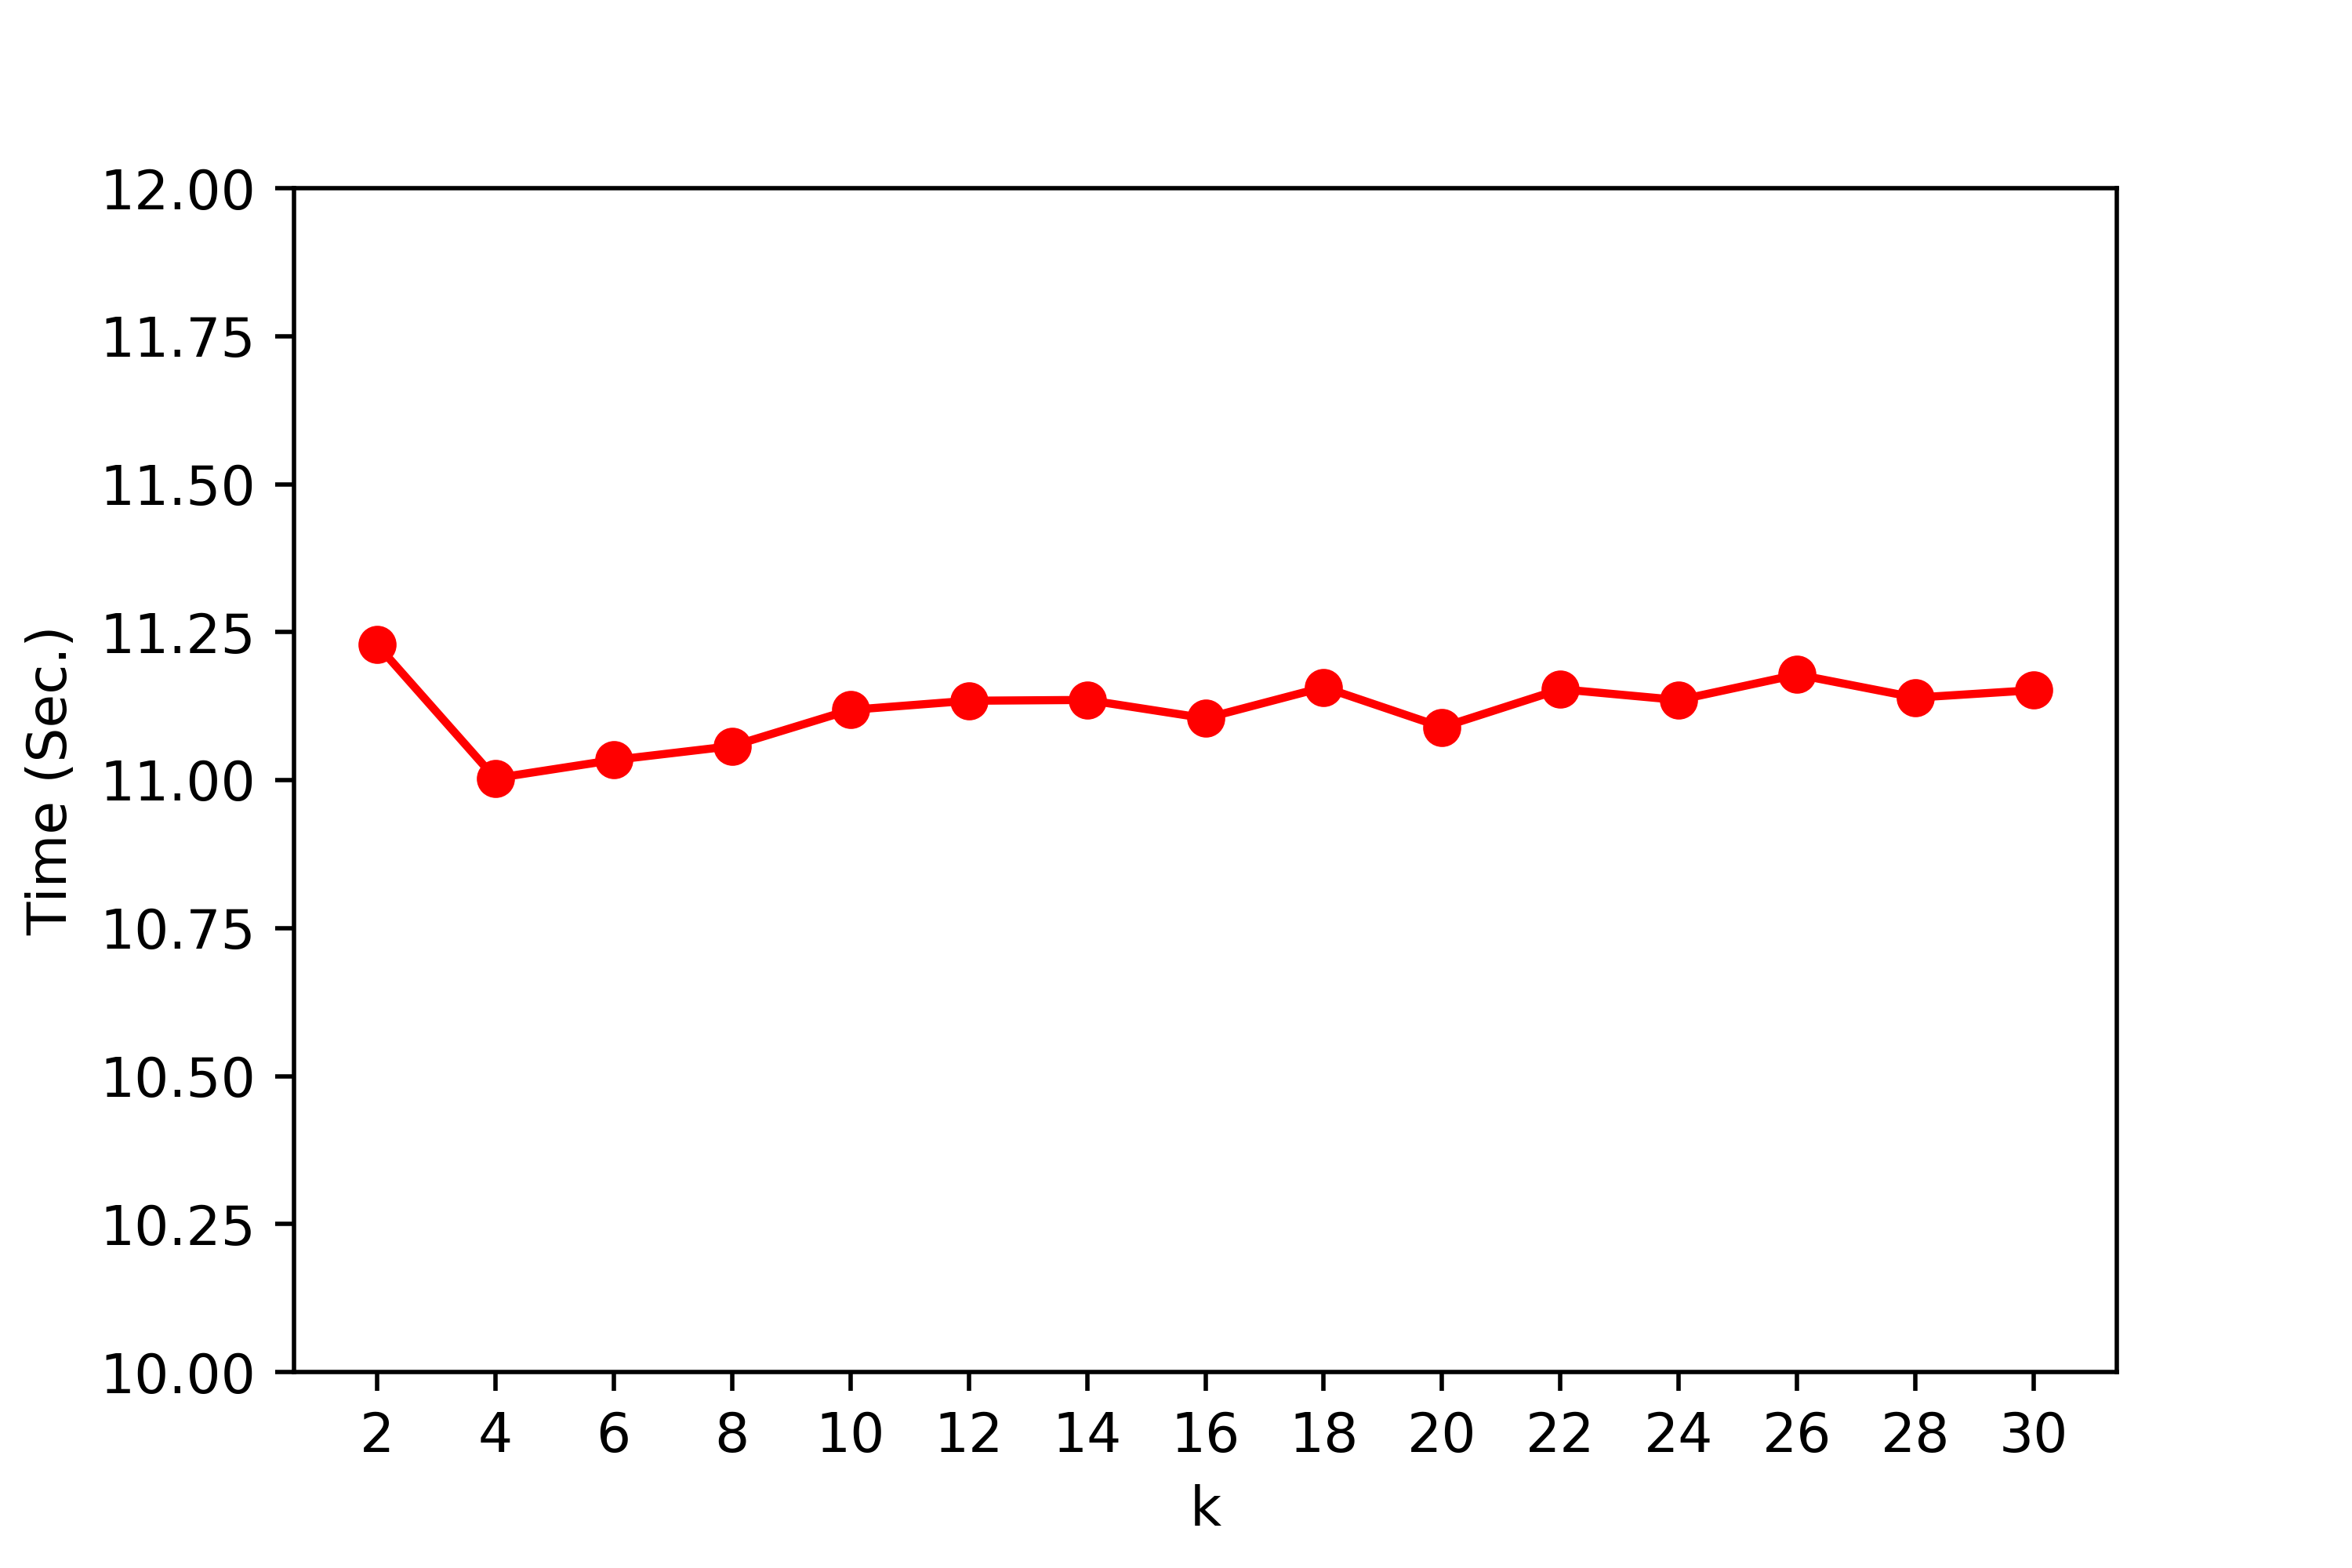
\includegraphics[scale=0.5]{KNN-LSTSVM-k}
	\caption{تاثیر پارامتر \lr{k} روی زمان آموزش روش \lr{KNN-LSTSVM}}
	\label{fig:KNN-LSTSVM-k}
\end{figure}

\newpage

\section{ارزیابی روش \lr{RKNN-TSVM}}\label{sec:5:3}
در این زیر بخش، ابتدا نحوه پیاده‌سازی و اجرای الگوریتم‌ها شرح داده شده است. سپس نحوه انتخاب پارامترهای بهینه توضیح داده شده است. در زیر بخش ، روش \lr{RKNN-TSVM} روی مجموعه داده‌های مصنوعی و واقعی به طور جامع بررسی می‌شود.

\subsection{نحوه پیاده‌سازی و اجرای الگوریتم‌ها}\label{sec:5:3:1}
نرم افزار  \lr{LightTwinSVM} برای اجرای روش \lr{TSVM} در بخش ‏\ref{sec:5:3} مورد استفاده قرار گرفته است. این نرم افزار شامل پیاده‌سازی ساده و سریع روش \lr{TSVM} می‌باشد که به عنوان بخشی از این پژوهش به طور رایگان در اختیار عموم قرار گرفته است\LTRfootnote{https://github.com/mir-am/LightTwinSVM}. روش \lr{RKNN-TSVM} و سایر روش‌ها در زبان برنامه‌نویسی پایتون نسخه \lr{3.5} پیاده‌سازی شده و همچنین الگوریتم \lr{clipDCD} و \lr{LDMDBA} در زبان برنامه‌نویسی \lr{C++} پیاده‌سازی شده است. تمامی آزمایش‌ها روی یک کامپیوتر شخصی با پردازنده \lr{Core i7 6700K}، سیستم عامل \lr{Ubuntu 16.04 LTS} و 32 گیگابایت حافظه انجام شده است. کتابخانه و نرم افزار‌های استفاده شده برای آزمایش روش \lr{RKNN-TSVM} را نشان می‌دهد. جدول \ref{tab:7} کتابخانه و نرم افزارهای استفاده شده برای آزمایش روش \lr{RKNN-TSVM} را نشان می‌دهد.


\begin{table}[!h]
	\small
	\centering
	\caption{کتابخانه و نرم افزارهای استفاده شده برای ارزیابی روش \lr{RKNN-TSVM}}
	\begin{tabular}{l c c c}
		\toprule
		% after \\: \hline or \cline{col1-col2} \cline{col3-col4} ...
		کتابخانه/نرم افزار & توضیح \\
		\midrule
		\lr{NumPy} \cite{walt2011} & اعمال جبر خطی در پایتون مانند ضرب و معکوس ماتریس \\
		\lr{SciPy} \cite{jones2014} & محاسبه فاصله و توابع آماری  \\
		\lr{Scikit-learn} \cite{pedregosa2011} & یادگیری ماشین و ارزیابی دسته‌بندها  \\
		\lr{GCC}\footnote{\lr{GNU Compiler Collection}} & کامپایلر برای زبان برنامه‌نویسی \lr{C++}   \\
		\lr{Pybind11}\footnote{\lr{https://pybind11.readthedocs.io/en/master/index.html}} & اجرای کد \lr{C++} در پایتون  \\
	
		\bottomrule
	\end{tabular}
	\label{tab:7}
\end{table}

\subsection{نحوه انتخاب پارامترها}\label{sec:5:3:2}
 همانطور که در زیر بخش \ref{sec:5:2:1} ذکر شد، عملکرد روش \lr{TSVM} و گسترش‌هایش بسیار وابسته به پارامترهای بهینه است. روش جستجوی شبکه‌ای برای انتخاب پارامترهای بهینه در آزمایش‌های بخش ‏\ref{sec:5:3} استفاده شده است. تابع \lr{RBF} به عنوان تابع هسته   $k(x_i, x_j)=\exp({-\left\|x_i - x_j\right\|^2}/\sigma^2)$ در نسخه غیر خطی بکار گرفته شده است. پارامتر تابع هسته  $\sigma$ از مجموعه  $\{2^{i} \mid i=-10,-9,\dots,2 \}$ انتخاب شده است. مقادیر بهینه پارامترهای  $c_{1}$،  $c_{2}$ و   $c_{3}$ از مجموعه   $\{2^{i} \mid i=-8,-7,\dots,2 \}$ تعیین شده است. به منظور کاهش بار محاسباتی انتخاب پارامترها،  $c_{1}=c_{2}$ و  $c_{3}=c_{4}$ در روش \lr{TBSVM}  و  $c_{2}=c_{3}$ در روش \lr{RKNN-TSVM} مساوی قرار داده شده است. همچنین مقدار بهینه پارامتر  $k$ از مجموعه   $\{2,3,\dots,15\}$ مشخص شده است.
 
\subsection{نتایج ارزیابی و بحث}\label{sec:5:3:3}
 در این زیر بخش، روش پیشنهادی (\lr{RKNN-TSVM}) روی مجموعه داده‌های مختلف مصنوعی و واقعی از نظر دقت و سرعت یادگیری بررسی می‌شود.
 
\subsubsection{مجموعه داده مصنوعی}\label{sec:5:3:3:1}
 به منظور نشان دادن برتری روش پیشنهادی نسبت به روش \lr{WLTSVM} به صورت هندسی، آزمایش روی دو مجموعه داده مصنوعی صورت گرفته است. 70 درصد نمونه‌های این مجموعه داده‌ها برای آموزش دسته‌بند به صورت تصادفی انتخاب شده است.
 
 در مثال اول، مجموعه داده مصنوعی \lr{Ripley} با 250 نمونه استفاده شده است. شکل ‏\ref{fig:WLTSVM-vs-RKNN-TSVM-R} ناحیه تصمیم روش \lr{WLTSVM} و \lr{RKNN-TSVM} را روی مجموعه داده \lr{Ripley} با تابع هسته خطی را نشان می‌دهد. همانطور که در شکل \ref{fig:WLTSVM-vs-RKNN-TSVM-R} مشخص است، روش پیشنهادی دقت بیشتری نسبت به روش \lr{WLTSVM} دارد. زیرا روش پیشنهادی به نمونه‌ها براساس فاصله نزدیک‌ترین همسایه‌هایش وزن می‌دهد. همچنین ابرصفحه‌ها در روش \lr{RKNN-TSVM} به نمونه‌های پرتراکم نزدیک‌تر دارد. 
 
 \begin{figure}[!t]
 	\centering
 	\subfloat[نسخه خطی \lr{WLTSVM} ($c=2^{3}, k=2$)]{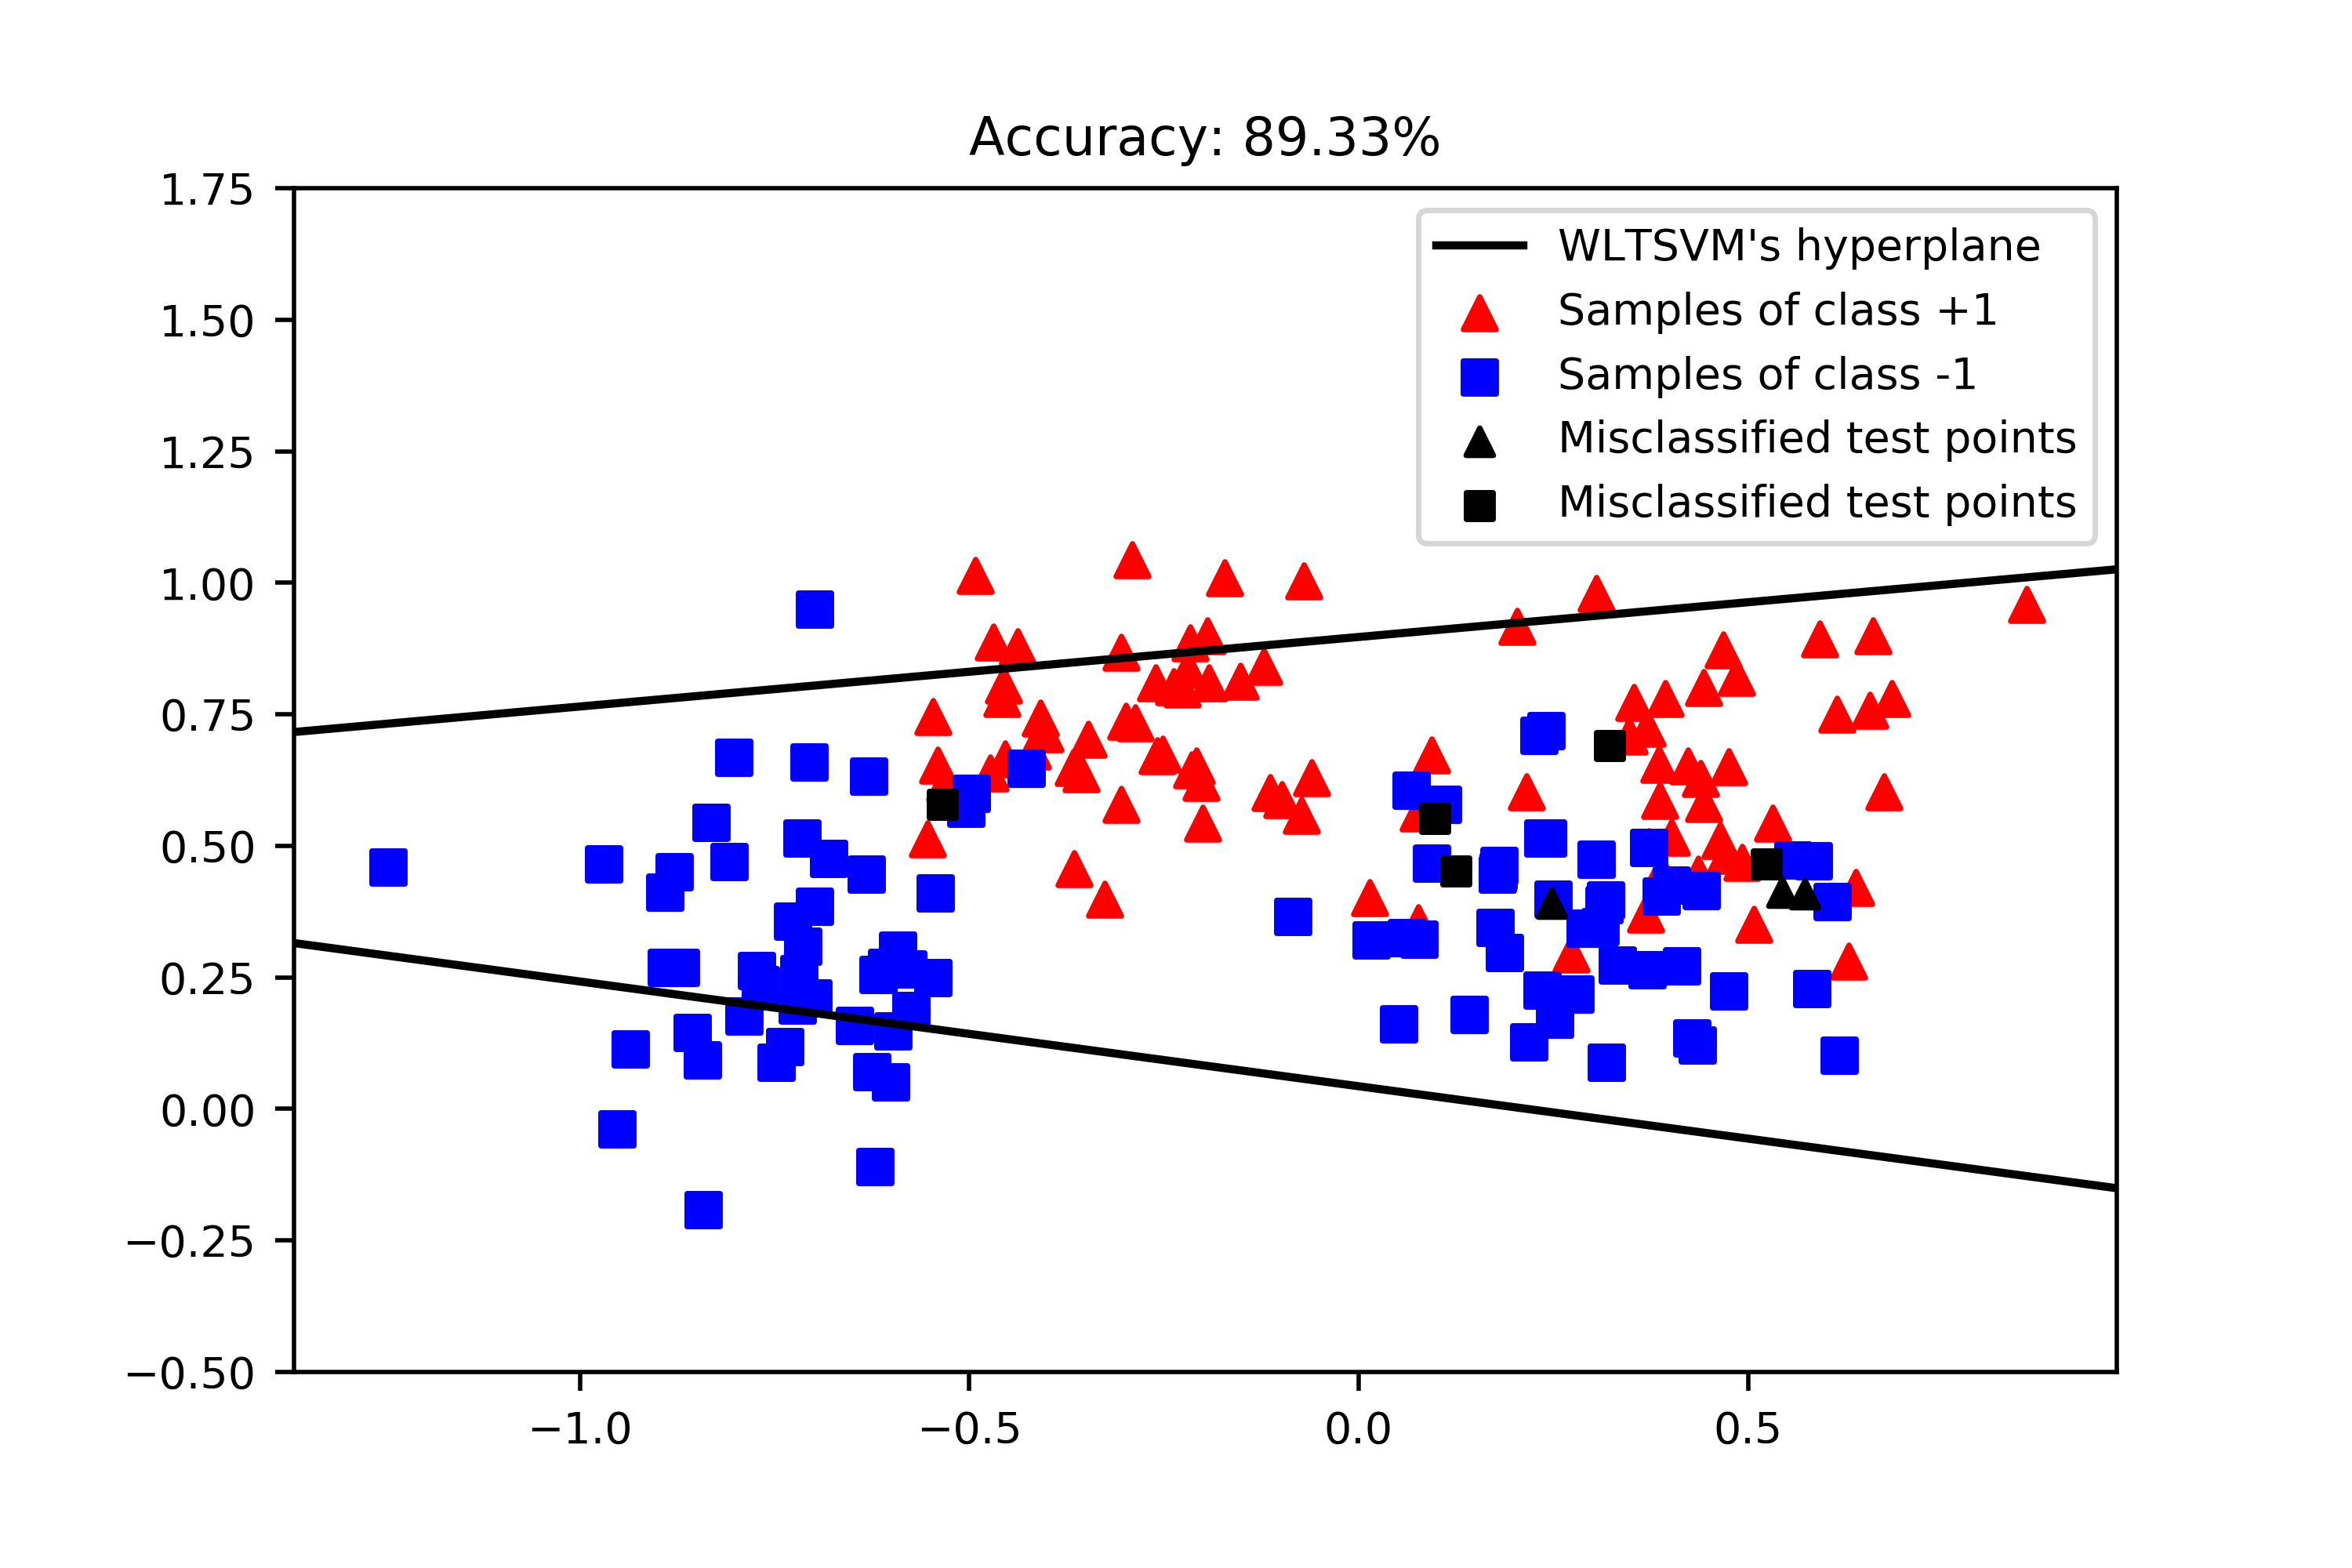
\includegraphics[width=0.5\textwidth]{WLTSVM-Ripley}}
 	\subfloat[نسخه خطی \lr{RKNN-TSVM} ($c_{1}=2^{2}, c_{2}=2^{-7}, c_{3}=2^{-2}, k=6$)]{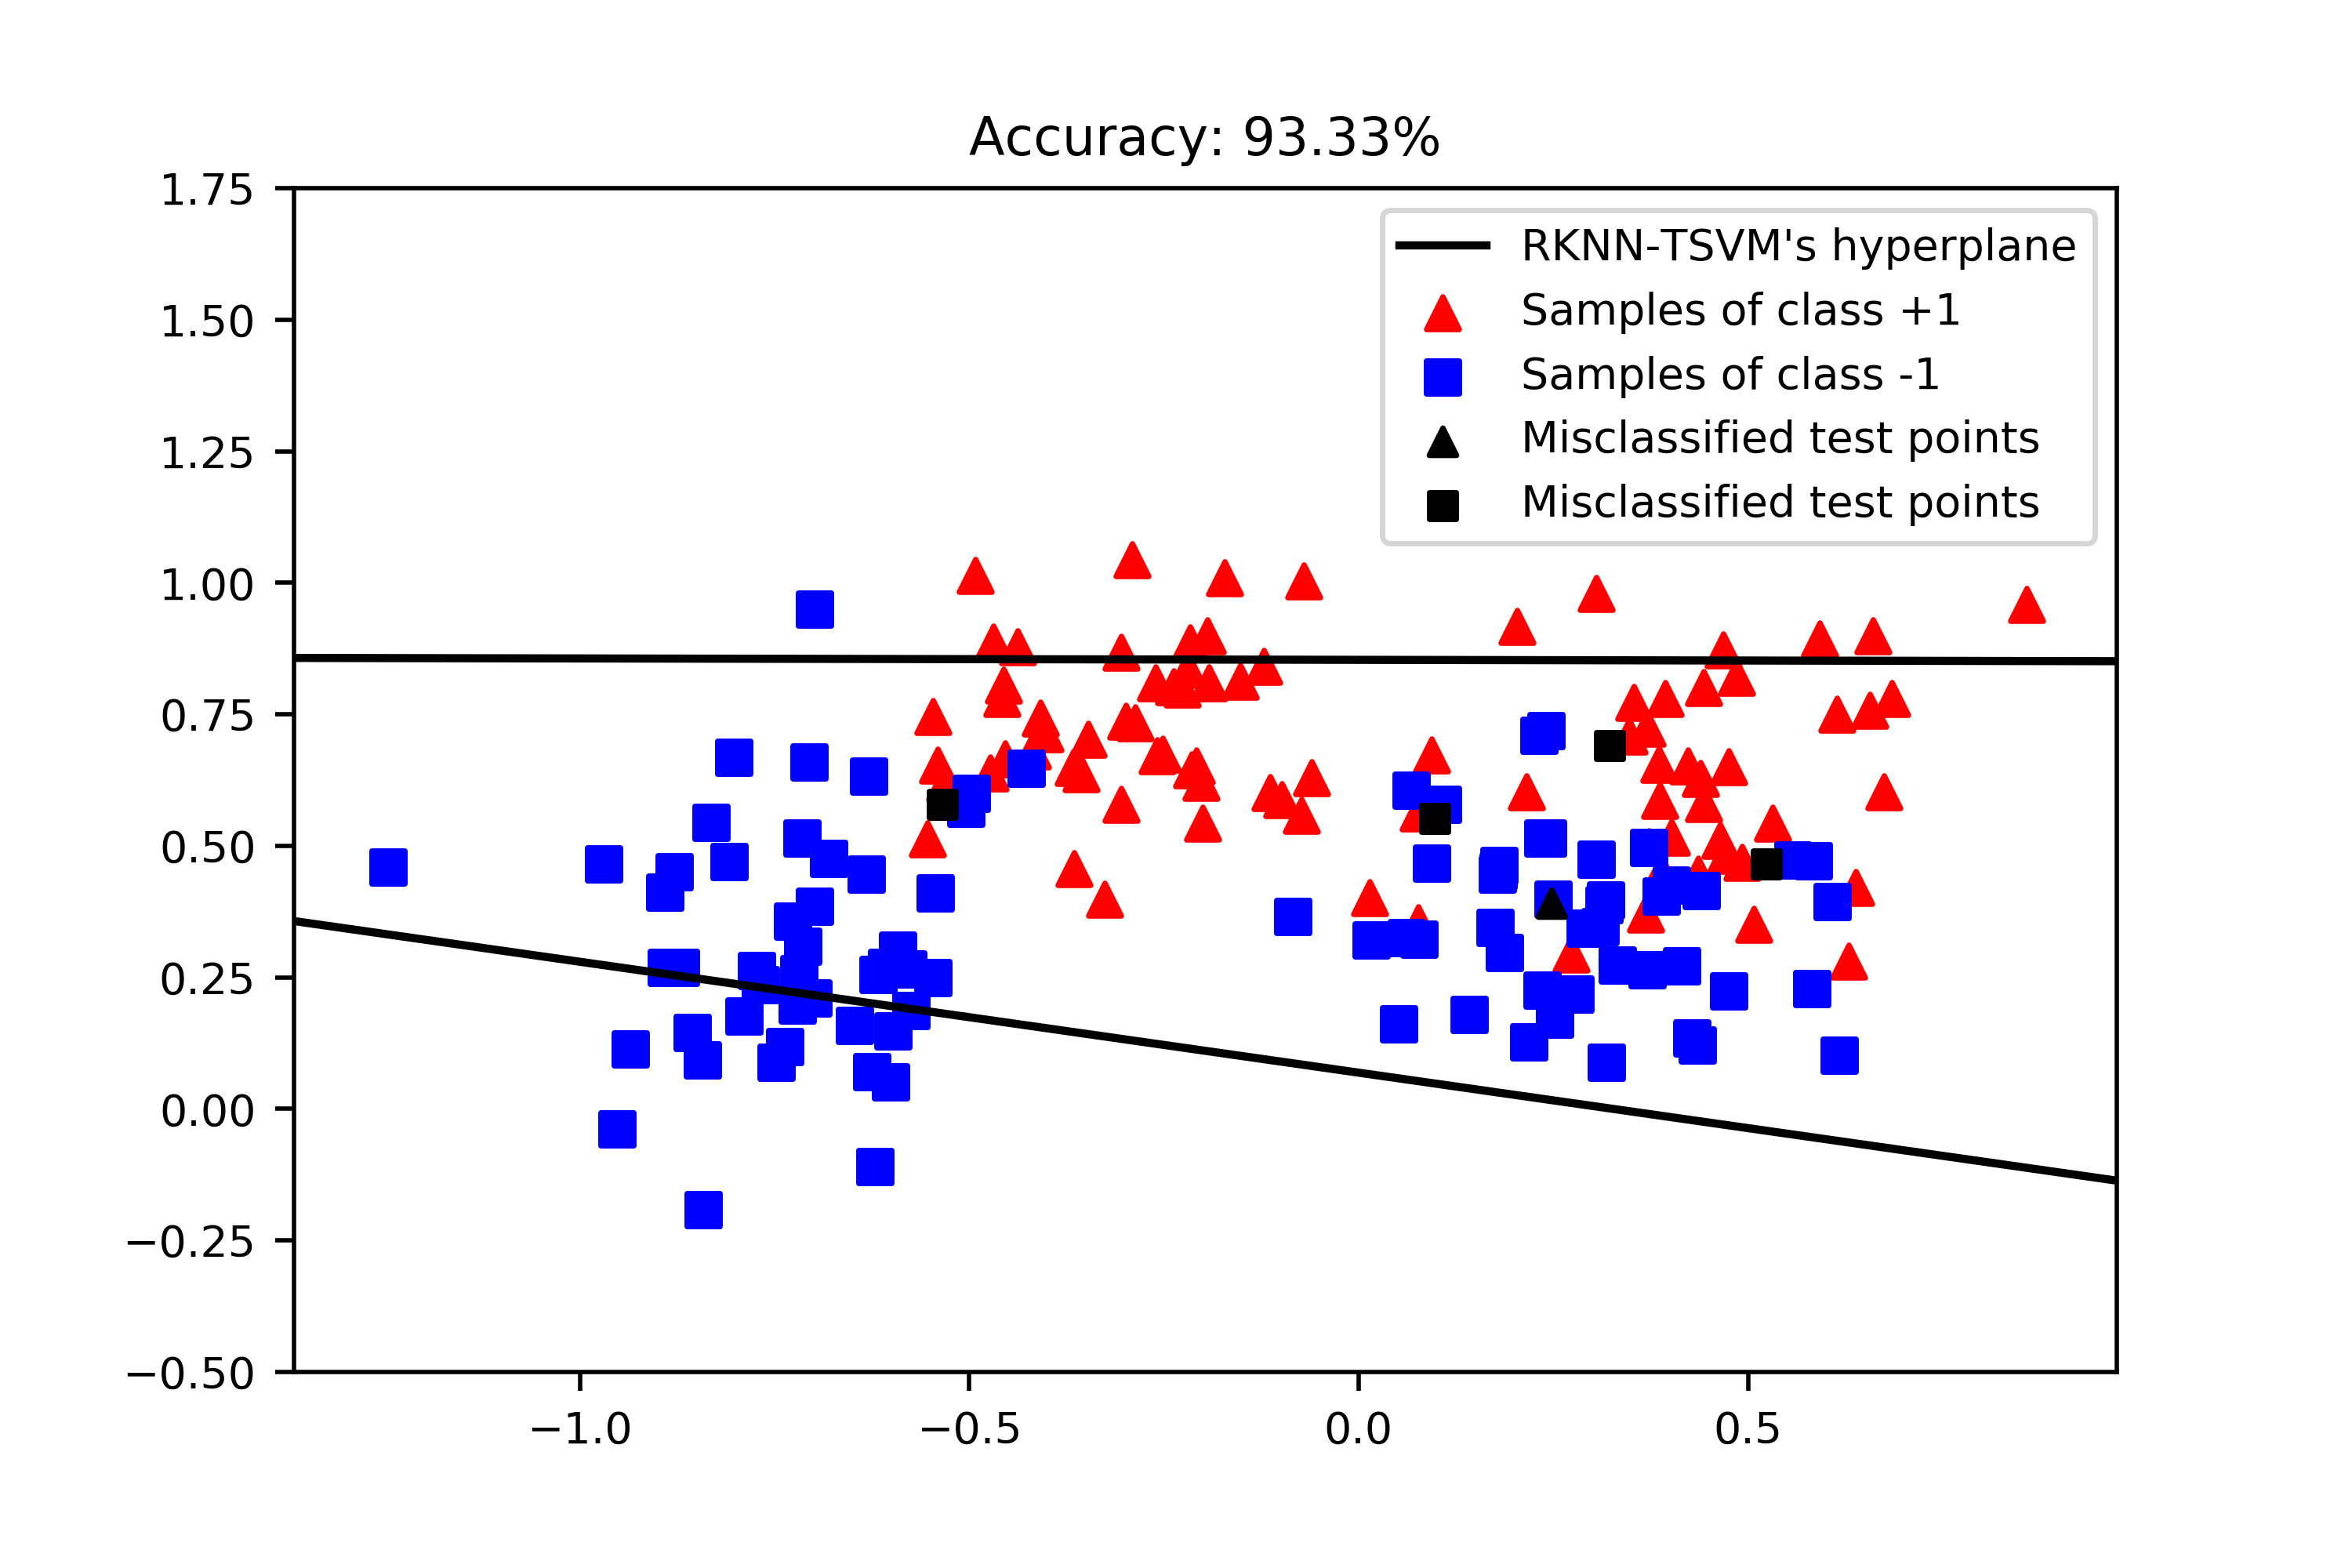
\includegraphics[width=0.5\textwidth]{RKNN-TSVM-Ripley}}
 	\caption{ناحیه تصمیم روش \lr{WLTSVM} و \lr{RKNN-TSVM} روی مجموعه داده \lr{Ripley} با تابع هسته خطی}
 	\label{fig:WLTSVM-vs-RKNN-TSVM-R}
 \end{figure}
\begin{figure}[!t]
	\centering
	\subfloat[نسخه غیر خطی \lr{WLTSVM} ($c=2^{-3}, k=8, \sigma=2^{0}$)]{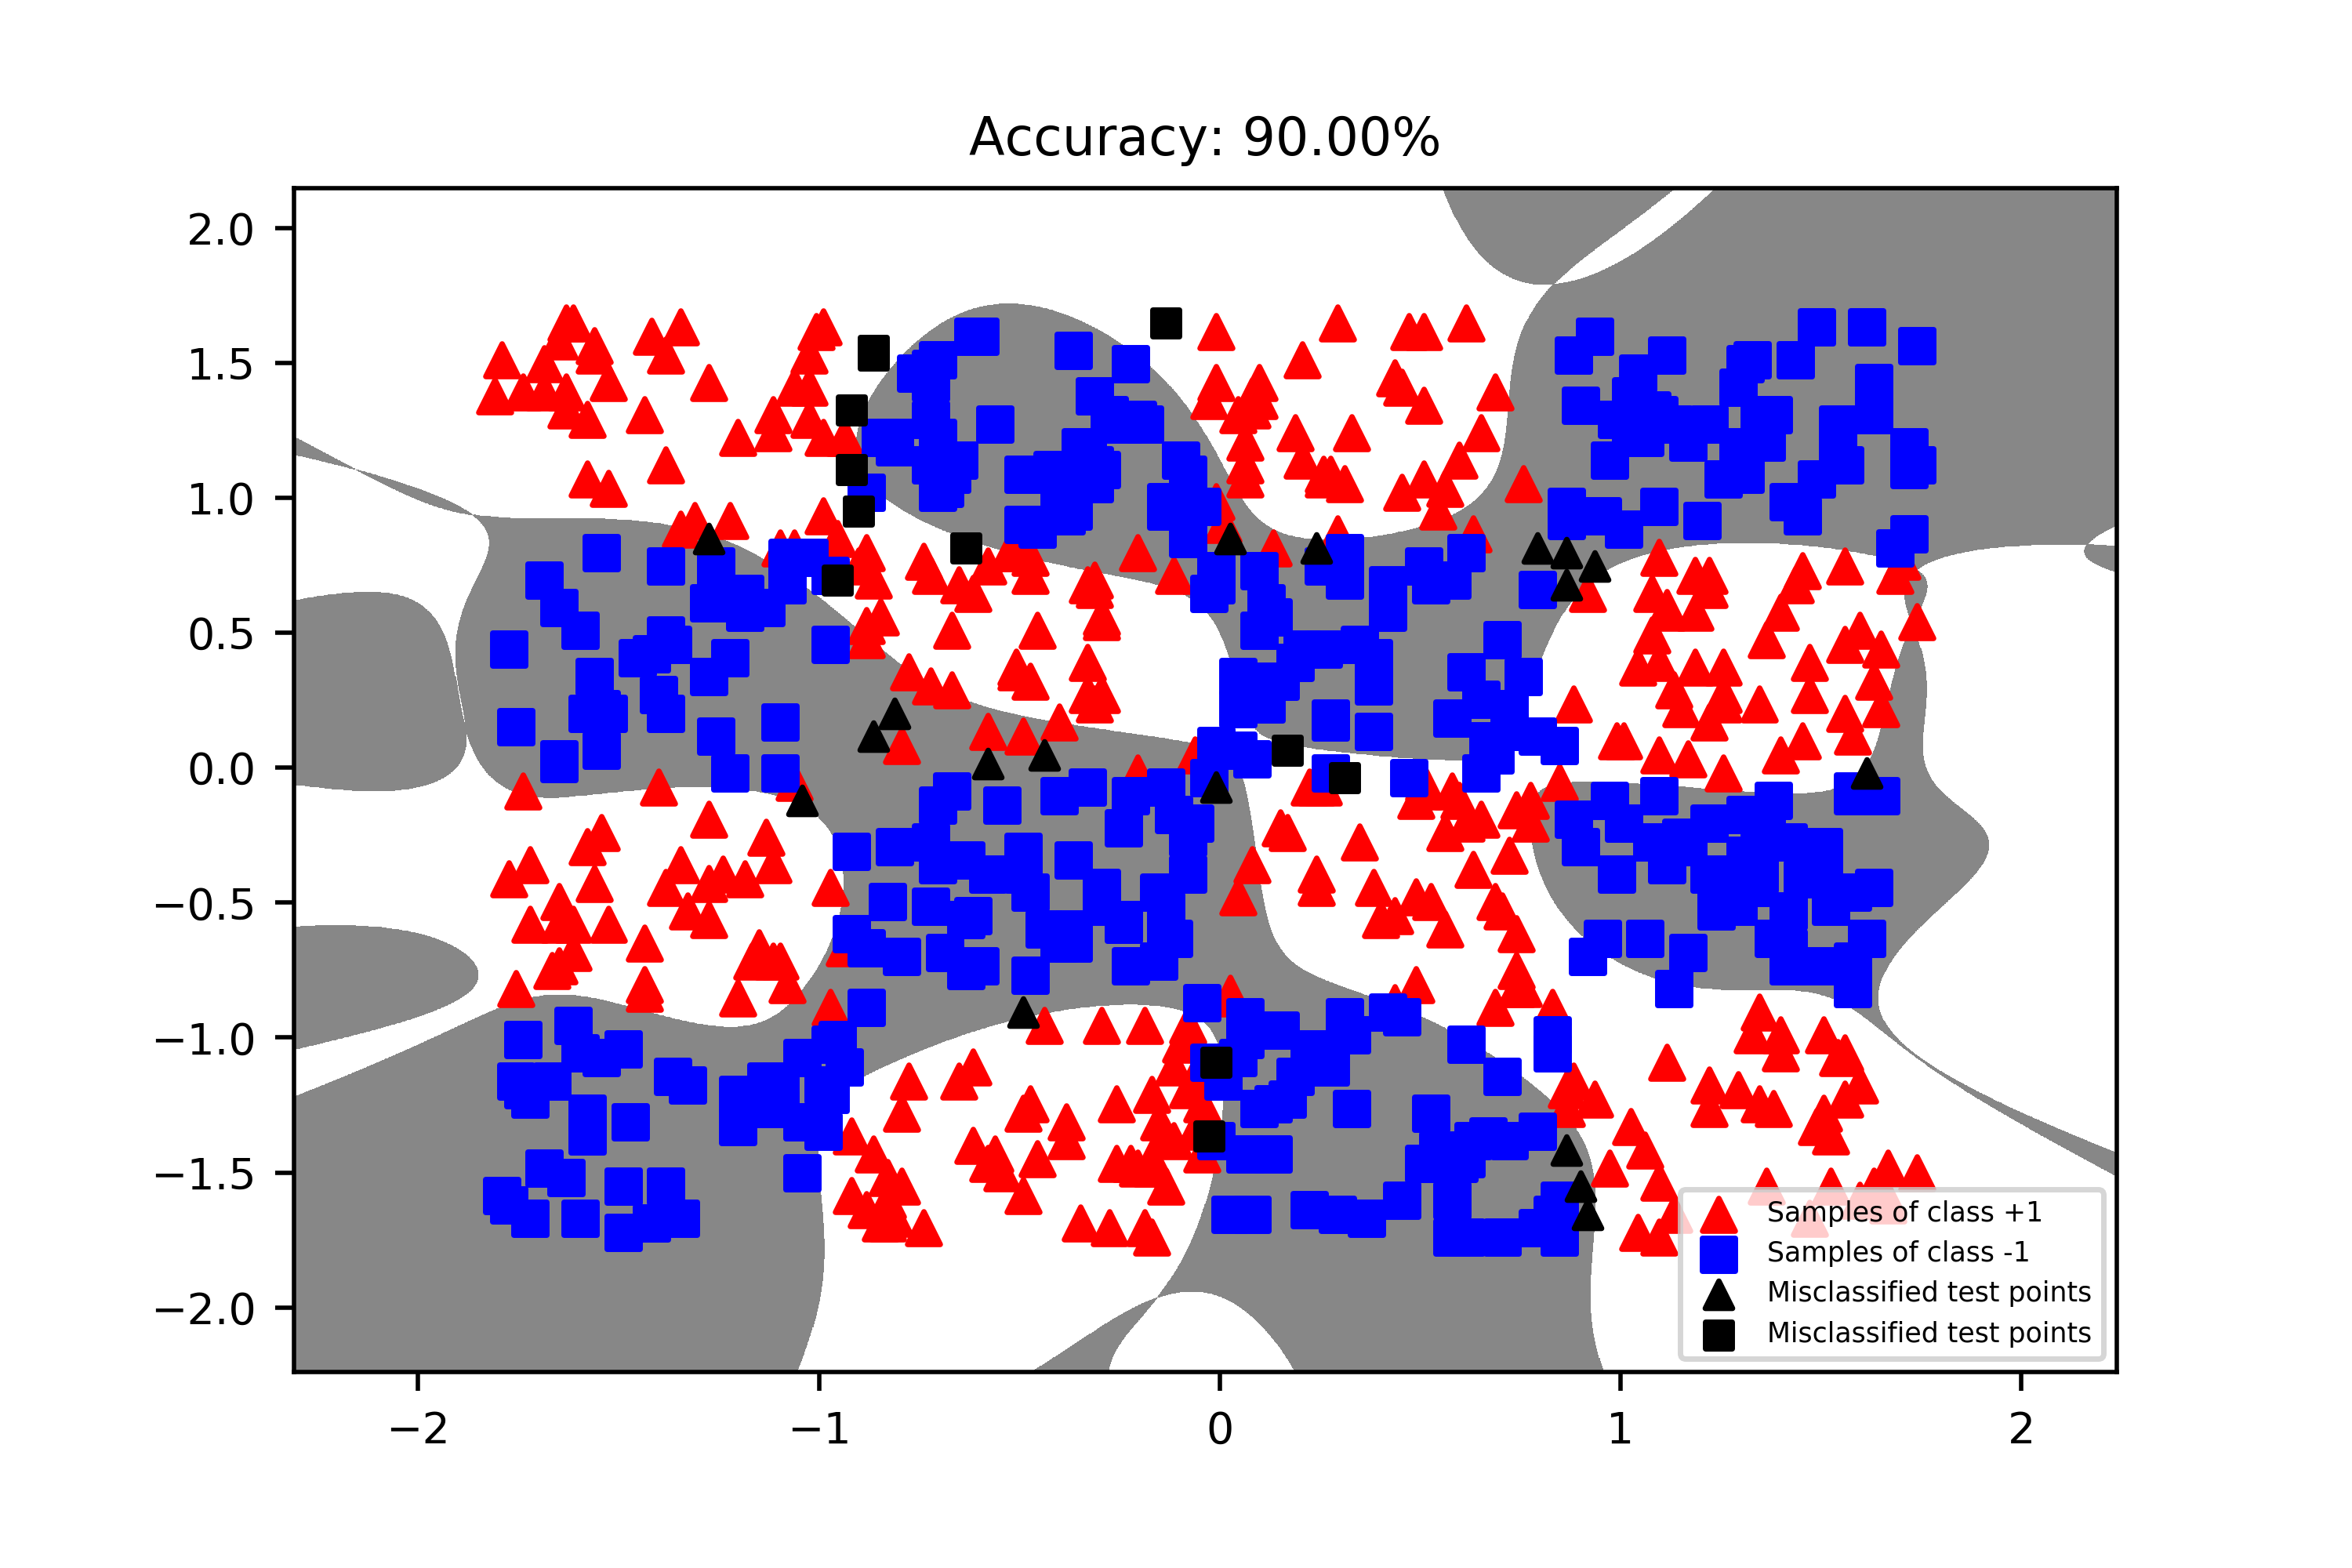
\includegraphics[width=0.5\textwidth]{WLTSVM-Check}}
	\subfloat[نسخه غیر خطی \lr{RKNN-TSVM} ($c_{1}=2^{-7}, c_{2}=2^{-6}, c_{3}=2^{-6}, k=10, \sigma=2^{1}$)]{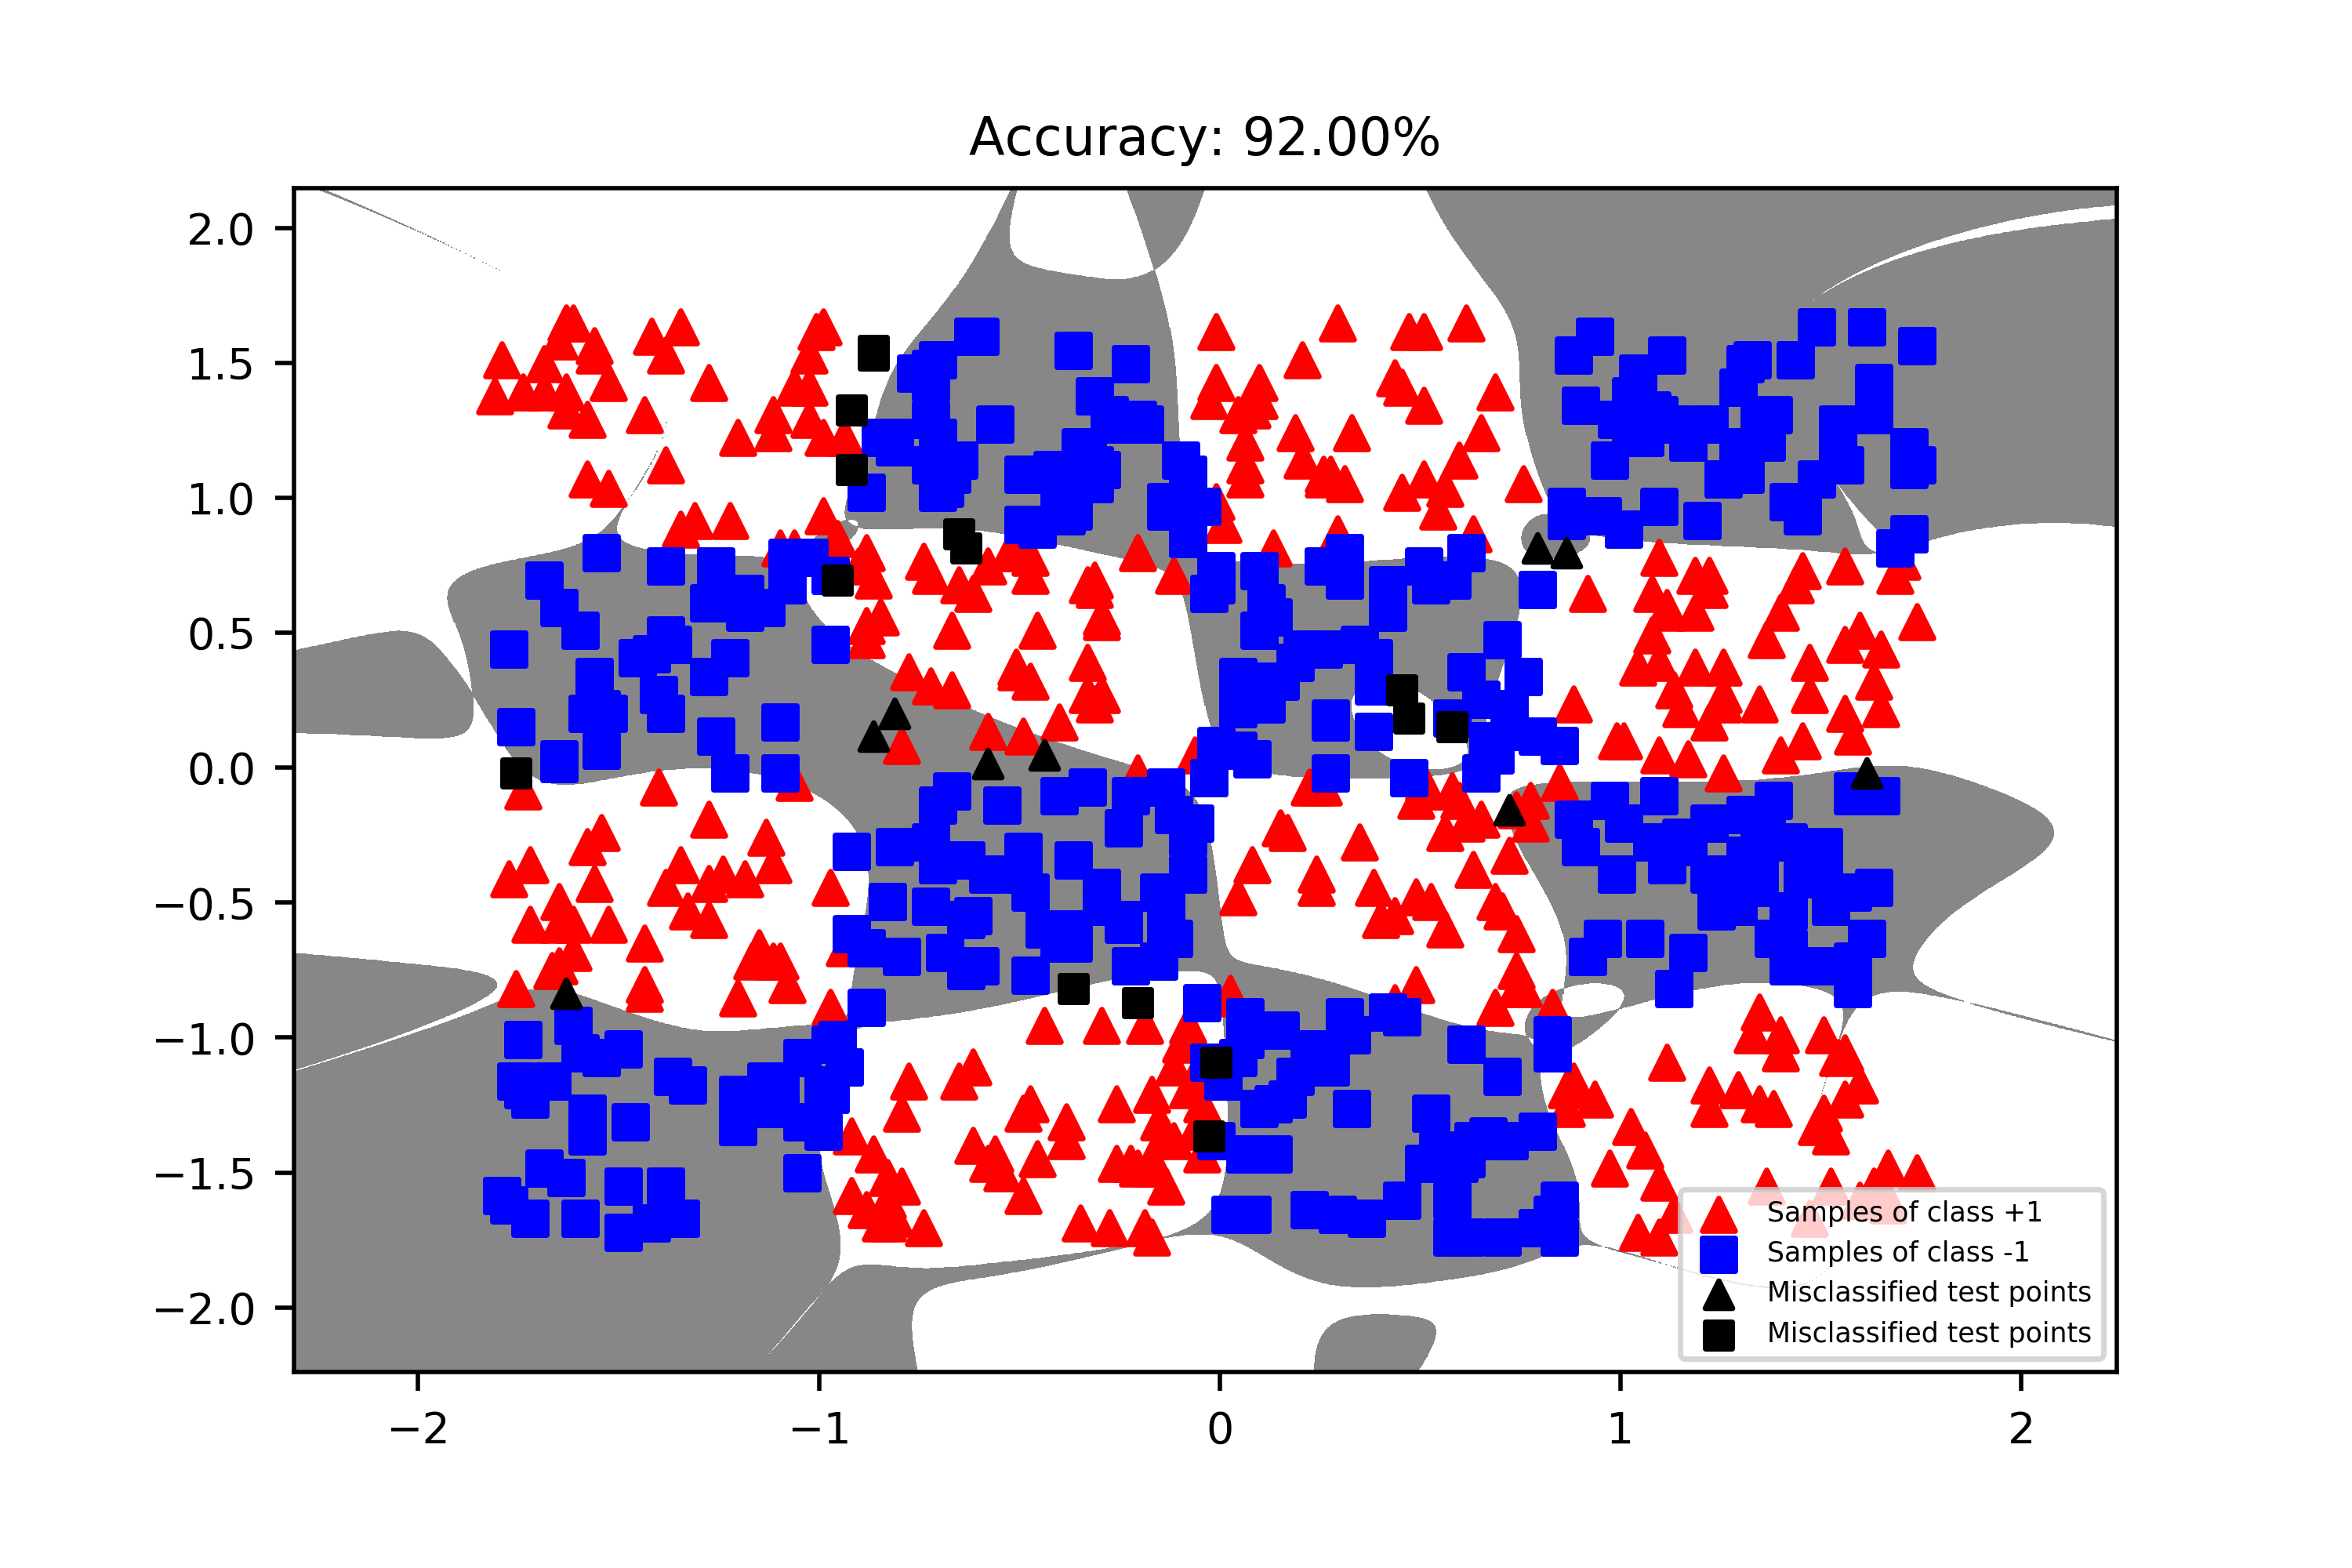
\includegraphics[width=0.5\textwidth]{RKNN-TSVM-Check}}
	\caption{ناحیه تصمیم روش  \lr{WLTSVM} و \lr{RKNN-TSVM} روی مجموعه داده \lr{Checkerboard} با تابع هسته \lr{RBF}}
	\label{fig:WLTSVM-vs-RKNN-TSVM-C}
\end{figure}

در مثال دوم، مجموعه داده مصنوعی \lr{Checkerboard} با 1000 نمونه استفاده شده است. شکل \ref{fig:WLTSVM-vs-RKNN-TSVM-C} ناحیه تصمیم روش \lr{WLTSVM} و \lr{RKNN-TSVM} را روی مجموعه داده \lr{Checkerboard} با تابع هسته \lr{RBF} را نشان می‌دهد. دقت نسخه غیر خطی روش پیشنهادی از نسخه غیر خطی روش \lr{WLTSVM} روی این مجموعه داده بیشتر است. زیرا روش پیشنهادی ریسک ساختاری را کمینه می‌کند و همچنین وزن‌دهی به نمونه‌ها براساس فاصله‌شان از نزدیک همسایه‌ها می‌باشد.

\subsubsection{مجموعه داده \lr{UCI}}\label{sec:5:3:3:2}
به منظور بررسی بیشتر عملکرد روش پییشنهادی (\lr{RKNN-TSVM})، مقایسه‌ای با روش‌های \lr{TSVM}، \lr{TBSVM} و \lr{WLTSVM} روی مجموعه داده‌های \lr{UCI} صورت گرفته است. لازم به ذکر است که تمامی مجموعه داده‌ها نرمال شده است. بطوریکه مقادیر ویژگی‌ها در بازه‌ی   $\left[0,1\right]$ قرار دارد. جدول \ref{tab:8} مشخصات این مجموعه داده‌ها را نشان می‌دهد.

\begin{table}[!t]
	\small
	\centering
	\caption{مشخصات مجموعه داده‌ها برای ارزیابی روش \lr{RKNN-TSVM}}
	\tabcolsep=0.11cm
	\begin{tabular}{l c c c c}
		\hline
		مجموعه داده & تعداد نمونه‌ها & نمونه‌های مثبت & نمونه‌های منفی & تعداد ویژگی‌ها \\
		\hline
\lr{{Australian}} & {690} & {307} & {383} & {14} \\
\lr{{Heart-Statlog}} & {270} & {120} & {150} & {13} \\
\lr{{Bupa-Liver}} & {345} & {145} & {200} & {6} \\
\lr{{WPBC}} & {198} & {47} & {151} & {33} \\
\lr{{WDBC}} & {569} & {212} & {357} & {30} \\
\lr{{Hepatitis}} & {155} & {32} & {123} & {19} \\
\lr{{Ionosphere}} & {351} & {225} & {126} & {34} \\
\lr{{Haberman}} & {306} & {225} & {81} & {3} \\
\lr{{Pima-Indian}} & {768} & {268} & {500} & {8} \\
\lr{{Fertility}} & {100} & {88} & {12} & {9} \\
\lr{{Votes}} & {435} & {267} & {168} & {16} \\
		
		\hline
	\end{tabular}
	\label{tab:8}
\end{table}

ارزیابی عملکرد روش‌ها و تنظیم کردن پارامترها با اعتبارسنج ضربدری 5 تایی انجام شده است. از این رو مجموعه داده به 5 بخش به صورت تصادفی تقسیم می‌شود و یکی از این زیربخش‌ها به عنوان نمونه‌های تست استفاده می‌گردد. فرآیند تقسیم‌بندی داده‌ها 5 بار تکرار می‌شود و میانگین این 5 بار به عنوان دقت دسته‌بند بشمار می‌رود.

دقت دسته‌بندی و زمان اجرای روش‌های \lr{TSVM}، \lr{TBSVM}، \lr{WLTSVM} و \lr{RKNN-TSVM} در جدول ذکر شده است. در اینجا دقت نشان دهنده میانگین نتایج روی داده‌های تست (به درصد) می‌باشد. زمان اجرا نیز به ثانیه است.

\begin{sidewaystable*}
	%\begin{table*}[!t]
	
	\small
	\centering
	\caption{مقایسه روش‌های \lr{TSVM}، \lr{TBSVM}، \lr{WLTSVM} و \lr{RKNN-TSVM} روی مجموعه داده‌های \lr{UCI} با تابع هسته \lr{RBF} }
	\ra{1.3} % Space between rows
	\tabcolsep=0.13cm % Adjusts column width
	%\begin{sideways}
	\begin{tabular}{p{2.70cm} \acol \tcol c \acol \tcol c \acol \tcol c \acol \tcol c \acol \tcol}
		\toprule
		
		% after \\: \hline or \cline{col1-col2} \cline{col3-col4} ...
		مجموعه داده  & \multicolumn{2}{c}{\lr{TSVM}} && \multicolumn{2}{c}{\lr{TBSVM}} && \multicolumn{2}{c}{\lr{WLTSVM}} && \multicolumn{2}{c}{\lr{RKNN-TSVM(FSA)}} && \multicolumn{2}{c}{\lr{RKNN-TSVM(LDMDBA)}} \\
		\cmidrule{2-3} \cmidrule{5-6} \cmidrule{8-9} \cmidrule{11-12} \cmidrule{14-15}
		($n\times d$) & دقت (\%) & زمان اجرا && دقت (\%) & زمان اجرا && دقت (\%) & زمان اجرا && دقت (\%) & زمان اجرا && دقت (\%) & زمان اجرا \\
		& $(c_{1}, c_{2}, \sigma)$  &  && $(c_{1}, c_{3}, \sigma)$  & && $(c, \sigma, k)$ &  && $(c_{1}, c_{2}, \sigma, k)$  &  && $(c_{1}, c_{2}, \sigma, k)$  &  \\
		\midrule
		\lr{Australian} & $87.10\pm3.09$ & $0.066$ && $87.39\pm3.39$ & $0.062$ && $86.52\pm3.53$ & $0.144$ && $87.54\pm3.65$ & $0.147$ && \textbf{$87.97\pm3.85$} & $0.226$ \\
		($690\times 14$) & ($2^{-4}, 2^{-5}, 2^{-7}$) &  && ($2^{-5}, 2^{2}, 2^{-6}$) &  && ($2^{2}, 2^{-8}, 14$) &  && ($2^{1}, 2^{-3}, 2^{-9}, 2$) &  && ($2^{-4}, 2^{-3}, 2^{-6}, 5$) & \\ 
		\lr{Heart-Statlog} & $84.81\pm2.72$ & $0.010$ && \textbf{$85.93\pm2.51$} & $0.013$ && $83.70\pm1.39$ & $0.023$ && \textbf{$85.93\pm3.01$} & $0.023$ && $85.56\pm2.16$ & $0.028$ \\
		($270\times 13$) & ($2^{0}, 2^{-1}, 2^{-10}$) &  && ($2^{0}, 2^{-3}, 2^{-10}$) &  && ($2^{0}, 2^{-7}, 12$) &  && ($2^{2}, 2^{-1}, 2^{-10}, 4$) &  && ($2^{1}, 2^{-5}, 2^{-10}, 5$) & \\ 
		\lr{Bupa-Liver} & \textbf{$74.78\pm2.35$} & $0.016$ && $73.62\pm2.13$ & $0.029$ && $73.91\pm2.05$ & $0.049$ && $73.91\pm4.30$ & $0.036$ && $73.91\pm4.58$ & $0.066$ \\
		($345\times 6$) & ($2^{1}, 2^{1}, 2^{-7}$) &  && ($2^{-2}, 2^{-7}, 2^{-5}$) &  && ($2^{0}, 2^{-6}, 10$) &  && ($2^{2}, 2^{-2}, 2^{-5}, 10$) &  && ($2^{2}, 2^{-3}, 2^{-5}, 7$) & \\ 
		\lr{WPBC} & $79.27\pm5.48$ & $0.017$ && $78.81\pm7.47$ & $0.012$ && $78.82\pm8.05$ & $0.016$ && $80.29\pm3.78$ & $0.013$ && \textbf{$80.32\pm3.98$} & $0.028$ \\
		($198\times 33$) & ($2^{-2}, 2^{-5}, 2^{-6}$) &  && ($2^{0}, 2^{-5}, 2^{-9}$) &  && ($2^{-3}, 2^{-7}, 7$) &  && ($2^{-1}, 2^{-2}, 2^{-5}, 11$) &  && ($2^{-2}, 2^{-5}, 2^{-6}, 10$) & \\ 
		\lr{WDBC} & $98.24\pm1.36$ & $0.072$ && $98.24\pm0.78$ & $0.055$ && $97.54\pm1.02$ & $0.090$ && \textbf{$98.59\pm0.70$} & $0.123$ && \textbf{$98.59\pm0.70$} & $0.157$ \\
		($569\times 30$) & ($2^{-4}, 2^{-2}, 2^{-9}$) &  && ($2^{-5}, 2^{-7}, 2^{-8}$) &  && ($2^{1}, 2^{-7}, 8$) &  && ($2^{-3}, 2^{-4}, 2^{-6}, 6$) &  && ($2^{0}, 2^{-3}, 2^{-7}, 8$) & \\ 
		\lr{Hepatitis} & $85.81\pm7.80$ & $0.004$ && $87.10\pm5.77$ & $0.004$ && $85.16\pm5.98$ & $0.012$ && $87.74\pm7.18$ & $0.017$ && \textbf{$88.39\pm6.95$} & $0.015$ \\
		($155\times 19$) & ($2^{-4}, 2^{-5}, 2^{-9}$) &  && ($2^{-5}, 2^{0}, 2^{-5}$) &  && ($2^{-5}, 2^{-7}, 11$) &  && ($2^{-4}, 2^{-3}, 2^{-6}, 7$) &  && ($2^{-4}, 2^{-3}, 2^{-6}, 3$) & \\ 
		\lr{Ionosphere} & $90.89\pm4.07$ & $0.031$ && $92.02\pm4.91$ & $0.015$ && $92.60\pm3.97$ & $0.057$ && \textbf{$93.73\pm3.45$} & $0.047$ && $93.17\pm3.87$ & $0.066$ \\
		($351\times 34$) & ($2^{-2}, 2^{-4}, 2^{-5}$) &  && ($2^{-8}, 2^{-5}, 2^{0}$) &  && ($2^{-5}, 2^{1}, 10$) &  && ($2^{-3}, 2^{1}, 2^{0}, 5$) &  && ($2^{-5}, 2^{2}, 2^{0}, 12$) & \\ 
		\lr{Haberman} & $75.46\pm5.06$ & $0.015$ && $75.82\pm3.17$ & $0.012$ && $76.11\pm7.36$ & $0.027$ && $76.77\pm5.30$ & $0.031$ && \textbf{$76.79\pm3.97$} & $0.049$ \\
		($306\times 3$) & ($2^{-2}, 2^{0}, 2^{-3}$) &  && ($2^{-3}, 2^{-4}, 2^{-3}$) &  && ($2^{0}, 2^{-6}, 11$) &  && ($2^{0}, 2^{-2}, 2^{-3}, 3$) &  && ($2^{0}, 2^{2}, 2^{-2}, 3$) & \\ 
		\lr{Pima-Indian} & $78.65\pm4.11$ & $0.089$ && $78.26\pm3.52$ & $0.059$ && $77.22\pm3.90$ & $0.193$ && $78.78\pm3.36$ & $0.191$ && \textbf{$78.91\pm2.45$} & $0.248$ \\
		($768\times 8$) & ($2^{-2}, 2^{-2}, 2^{-2}$) &  && ($2^{-1}, 2^{-6}, 2^{-2}$) &  && ($2^{2}, 2^{-3}, 10$) &  && ($2^{1}, 2^{-3}, 2^{-1}, 4$) &  && ($2^{2}, 2^{-2}, 2^{-1}, 7$) & \\ 
		\lr{Fertility} & $88.00\pm8.12$ & $0.003$ && $89.00\pm10.68$ & $0.002$ && $88.00\pm6.78$ & $0.005$ && $90.00\pm7.07$ & $0.005$ && \textbf{$91.00\pm3.74$} & $0.017$ \\
		($100\times 9$) & ($2^{-8}, 2^{-3}, 2^{-2}$) &  && ($2^{-8}, 2^{2}, 2^{1}$) &  && ($2^{-5}, 2^{1}, 2$) &  && ($2^{-3}, 2^{-1}, 2^{1}, 2$) &  && ($2^{-8}, 2^{-3}, 2^{-1}, 3$) & \\ 
		\lr{Votes} & $96.55\pm2.41$ & $0.047$ && \textbf{$97.01\pm2.00$} & $0.021$ && $96.55\pm2.91$ & $0.042$ && \textbf{$97.01\pm1.38$} & $0.040$ && \textbf{$97.01\pm1.56$} & $0.092$ \\
		($435\times 16$) & ($2^{-5}, 2^{-1}, 2^{-8}$) &  && ($2^{1}, 2^{-2}, 2^{-7}$) &  && ($2^{1}, 2^{-10}, 15$) &  && ($2^{2}, 2^{0}, 2^{-7}, 10$) &  && ($2^{2}, 2^{-5}, 2^{-9}, 11$) & \\
		&  &  && &  && &  &&  &  && & \\ 
		%\textbf{Win/draw/loss} &  &  && &  && &  &&  &  && & \\ 
		%\tiny RKNN-TSVM(LDMDBA) & 10/0/1  &  && 9/1/1 &  && 10/1/0 &  && 6/3/2 &  && & \\
		\midrule
		میانگین دقت & \multicolumn{2}{c}{$85.41$} && \multicolumn{2}{c}{$85.75$} && \multicolumn{2}{c}{$85.10$} && \multicolumn{2}{c}{$86.39$} && \multicolumn{2}{c}{\textbf{$86.51$}} \\
		\bottomrule
	\end{tabular}
	%\end{sideways}
	
	\label{tab:9}
	%\end{table*}
\end{sidewaystable*}

از جنبه دقت دسته‌بندی، روش پیشنهادی (\lr{RKNN-TSVM}) بهتر از سایر روش‌ها مانند \lr{TSVM} و \lr{WLTSVM} روی بیشتر مجموعه داده‌ها عمل کرده است. ويژگی‌های روش پیشنهادی باعث بهبود دقت شده است که در زیر توضیح داده شده است.
\begin{enumerate}
	\item روش پیشنهادی به نمونه‌ها بر اساس فاصله شان از نزدیک‌ترین همسایه‌ها وزن می‌دهد. در حالی‌که در روش  \lr{WLTSVM} صرفا  براساس شماره تعداد همسایه‌های نزدیک به نمونه وزن نسبت داده می‌شود. بطوریکه ماتریس وزن ها در روش \lr{WLTSVM} شامل مقادیر دودویی است.
	\item مشابه روش \lr{TBSVM}، روش پیشنهادی ریسک ساختاری را در مسئله بهینه سازی خود در نظر می‌گیرد. در حالی‌که روش‌های  \lr{TSVM}و  \lr{WLTSVM}ریسک تجربی را کمینه می‌کنند. به عبارت دیگر، مقادیر پارامترهای  $c_{2}$ و  $c_{3}$ دقت دسته بندی روش بهبود داده است. با این حال مقادیر این پارامتر در روش‌های \lr{TSVM} و \lr{WLTSVM} یک عدد ثابت بسیار کوچک است.
\end{enumerate}

با توجه به جدول \ref{tab:9}، نه تنها روش پیشنهادی با الگوریتم \lr{LDMDBA} از سایر روش‌های \lr{TSVM}، \lr{TBSVM} و \lr{WLTSVM} بهتر عمل کرده است، بلکه نسبت به روش پیشنهادی با الگوریتم \lr{FSA} نیز دقت بیشتری دارد. هدف از بکارگیری الگوریتم \lr{LDMDBA} بهبود سرعت آموزش روش ‍پیشنهادی بوده است. با این حال این الگوریتم دقت دسته‌بندی روش ‍پیشنهادی را هم افزایش داده است.

از جنبه زمان اجرا و سرعت آموزش، روش \lr{TSVM} از روش پیشنهادی و \lr{WLTSVM} سریع‌تر است. زیرا روش فقط دو مسئله دوگان را حل می‌کند. در حالی‌که در روش پیشنهادی و \lr{WLTSVM} علاوه بر حل کردن دو مسئله دوگان، نزدیک‌ترین همسایه‌های تمام نمونه‌ها باید محاسبه گردد. به منظور بهبود مرتبه زمانی روش پیشنهادی (\lr{RKNN-TSVM})، الگوریتم \lr{LDMDBA} برای ساخت گراف نزدیک‌ترین همسایه استفاده شده است. در بخش ، سرعت آموزش روش پیشنهادی بر روی مجموعه داده‌های بزرگ بررسی شده است.

شکل \ref{fig:RKNN-TSVM-k} تاثیر مقدار پارامتر $k$ روی زمان آموزش روش پیشنهادی با الگوریتم \lr{FSA} و \lr{LDMDBA} روی مجموعه داده \lr{Pima-Indian} را نشان می‌دهد. همانطور که در شکل \ref{fig:RKNN-TSVM-k} مشخص است، زمان آموزش روش پیشنهادی با افزایش مقدار $k$ بیشتر می‌شود. با این حال روش پیشنهادی با الگوریتم \lr{LDMDBA} به طور قابل توجه‌ای از الگوریتم \lr{FSA} برای هر تمامی مقادیر سریع‌تر است.

\begin{figure}[!t]
	\centering
	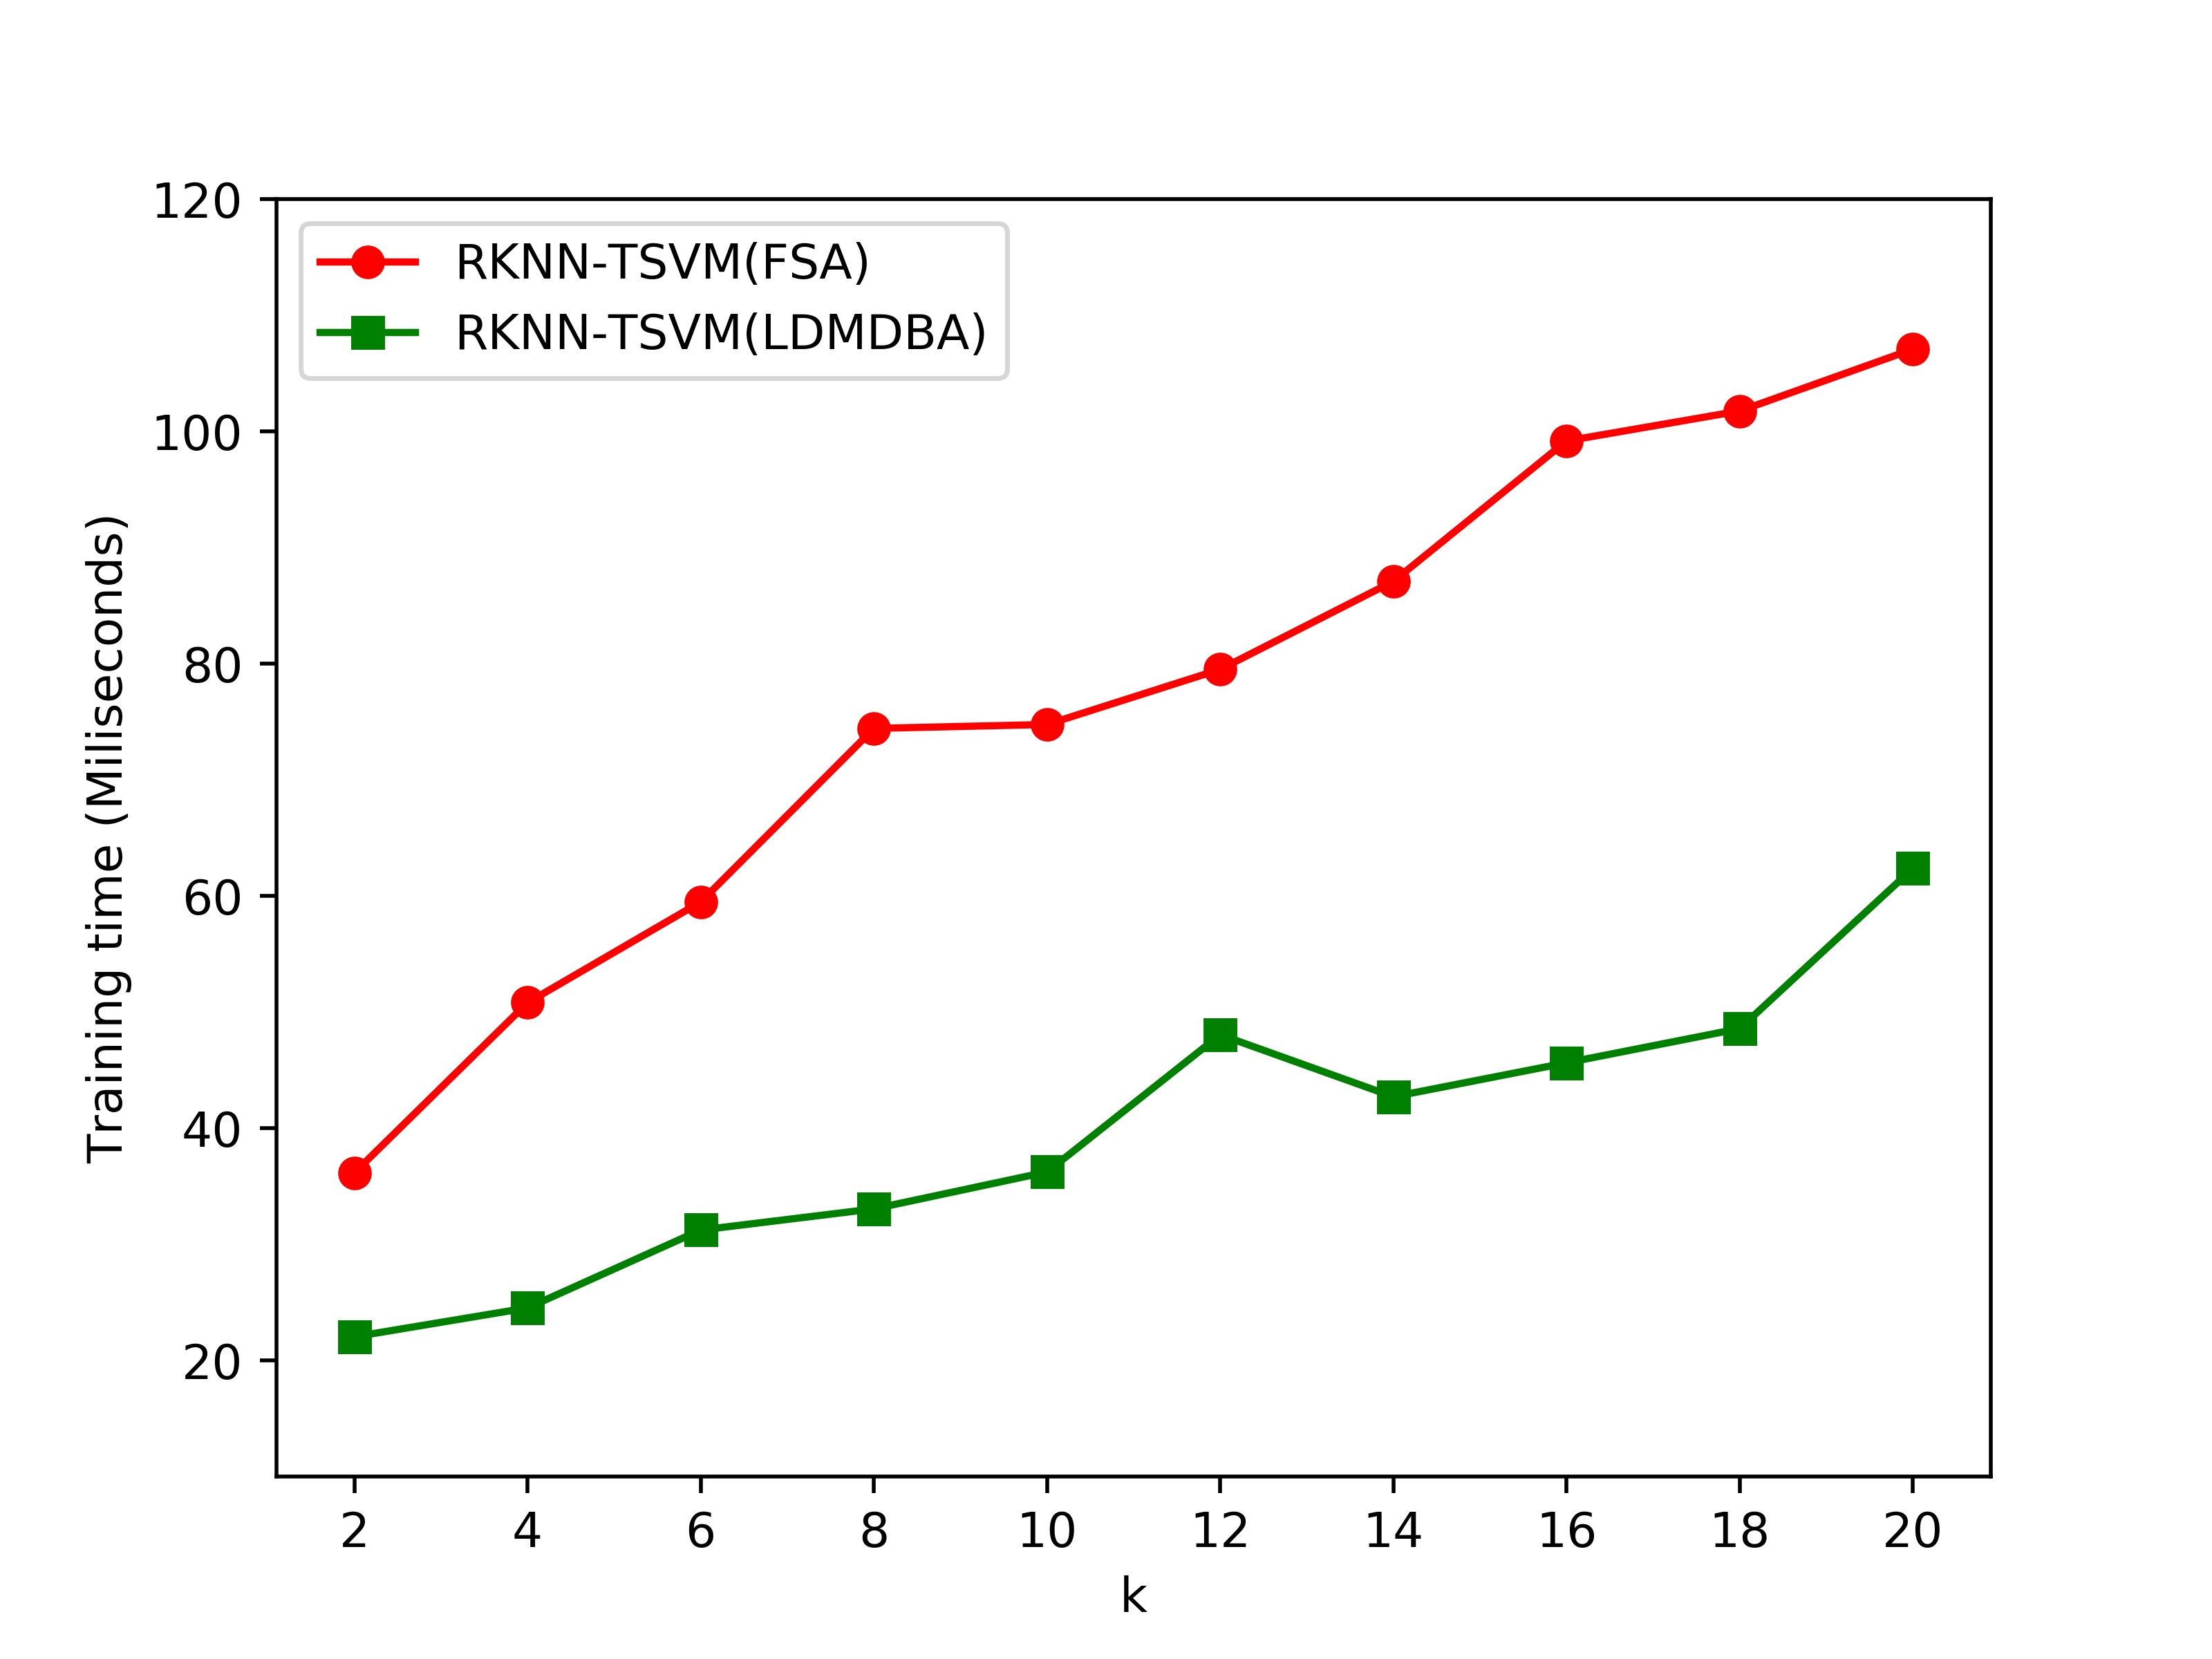
\includegraphics[scale=0.5]{RKNN-TSVM-k}
	\caption{تاثیر پارامتر $k$ روی زمان آموزش روش \lr{RKNN-TSVM} روی مجموعه داده \lr{Pima-Indian} }
	\label{fig:RKNN-TSVM-k}
\end{figure}

\subsubsection{بررسی آماری}\label{sec:5:3:3:3}
به منظور تحلیل آماری عملکرد پنج دسته‌بند روی مجموعه داده‌های \lr{UCI}، آزمون فریدمن بکار گرفته شده است (نحوه محاسبه این آزمون آماری در بخش \ref{sec:5:2:3:1} بیان شده است.). بدین منظور میانگین رتبه پنج روش براساس دقت محاسبه شده و در جدول نمایش داده شده است. ابتدا فرض گرفته می‌شود که بر اساس فرضیه صفر تمام دسته‌بندها یکسان هستند.

\begin{table}[!t]
	\centering
	\caption{میانگین رتبه براساس دقت (ارزیابی \lr{RKNN-TSVM})}
	\ra{1.3} % Space between rows
	\tabcolsep=0.10cm
	\begin{tabular}{c c c c c c c c c c c c c}
		\toprule
		% after \\: \hline or \cline{col1-col2} \cline{col3-col4} ...
		مجموعه داده  & \lr{TSVM }& \lr{TBSVM} & \lr{WLTSVM} & \lr{RKNN-TSVM(FSA)} & \lr{RKNN-TSVM(LDMDBA) }\\
		\midrule
\lr{Australian} & 4 & 3 & 5 & 2 & 1\\ 
\lr{Heart-Statlog} & 4 & $1.5$ & 5 & $1.5$ & 3\\ 
\lr{Bupa-Liver} & 1 & 5 & 3 & 3 & 3\\ 
\lr{WPBC} & 3 & 5 & 4 & 2 & 1\\ 
\lr{WDBC} & $3.5$ & $3.5$ & 5 & $1.5$ & $1.5$\\ 
\lr{Hepatitis} & 4 & 3 & 5 & 2 & 1\\ 
\lr{Ionosphere} & 5 & 4 & 3 & 1 & 2\\ 
\lr{Haberman} & 5 & 4 & 3 & 2 & 1\\ 
\lr{Pima-Indian} & 3 & 4 & 5 & 2 & 1\\ 
\lr{Fertility} & $4.5$ & 3 & $4.5$ & 2 & 1\\ 
\lr{Votes} & $4.5$ & 2 & $4.5$ & 2 & 2\\ 
میانگین رتبه & $3.77$ & $3.45$ & $4.27$ & $1.91$ & \textbf{$1.59$} \\ 
		\bottomrule
	\end{tabular}
	
	\label{tab:10}
\end{table}

بعد از انجام آزمون آماری فریدمن، مقادیر $\chi^2_F = 24.636$ و $F_F = 12.723$ بدست آمده است. با در نظرگرفتن 5 دسته‌بند و 11 مجموعه داده، $F_F$ از توزیع $F$ با (4, 40) درجه آزادی پیروی می‌کند. مقادیر ویژه $F(4,40)$ برای سطوح معناداری $0.25$، $0.1$ و $0.05$ به ترتیب برابر با $1.40$، $2.09$ و $2.61$ است. مقدار $F_F$ به طور قابل توجه‌ای بیشتر از مقدار ويژه است. بنابر با توجه به نتایج آزمون آماری، فرضیه صفر رد می‌شود. در نتیجه تفاوت معنادار و قابل توجه‌ای بین ۵ دسته‌بند وجود دارد. همچنین جدول \ref{tab:10} نشان می‌دهد که روش پیشنهادی (\lr{RKNN-TSVM}) بهتر از سایر روش ها عمل کرده است. زیرا میانگین رتبه روش پیشنهادی در میان سایر روش‌ها کمترین است.

\subsubsection{بررسی حساسیت روش \lr{RKNN-TSVM} به پارامترها}\label{sec:5:3:3:4}
به منظور دست‌یابی به دقت بهتر، انتخاب پارامترهای بهینه برای روش پیشنهادی اهمیت زیادی دارد. آزمایش روی دو مجموعه داده \lr{Australian} و \lr{Hepatitis} صورت گرفته است تا حساسیت روش پیشنهادی به پارامترهای $c_{1}$، $c_{2}$ و $k$ بررسی شود.

\begin{figure}[!t]
	\centering
	\subfloat[مجموعه داده \lr{Australian}]{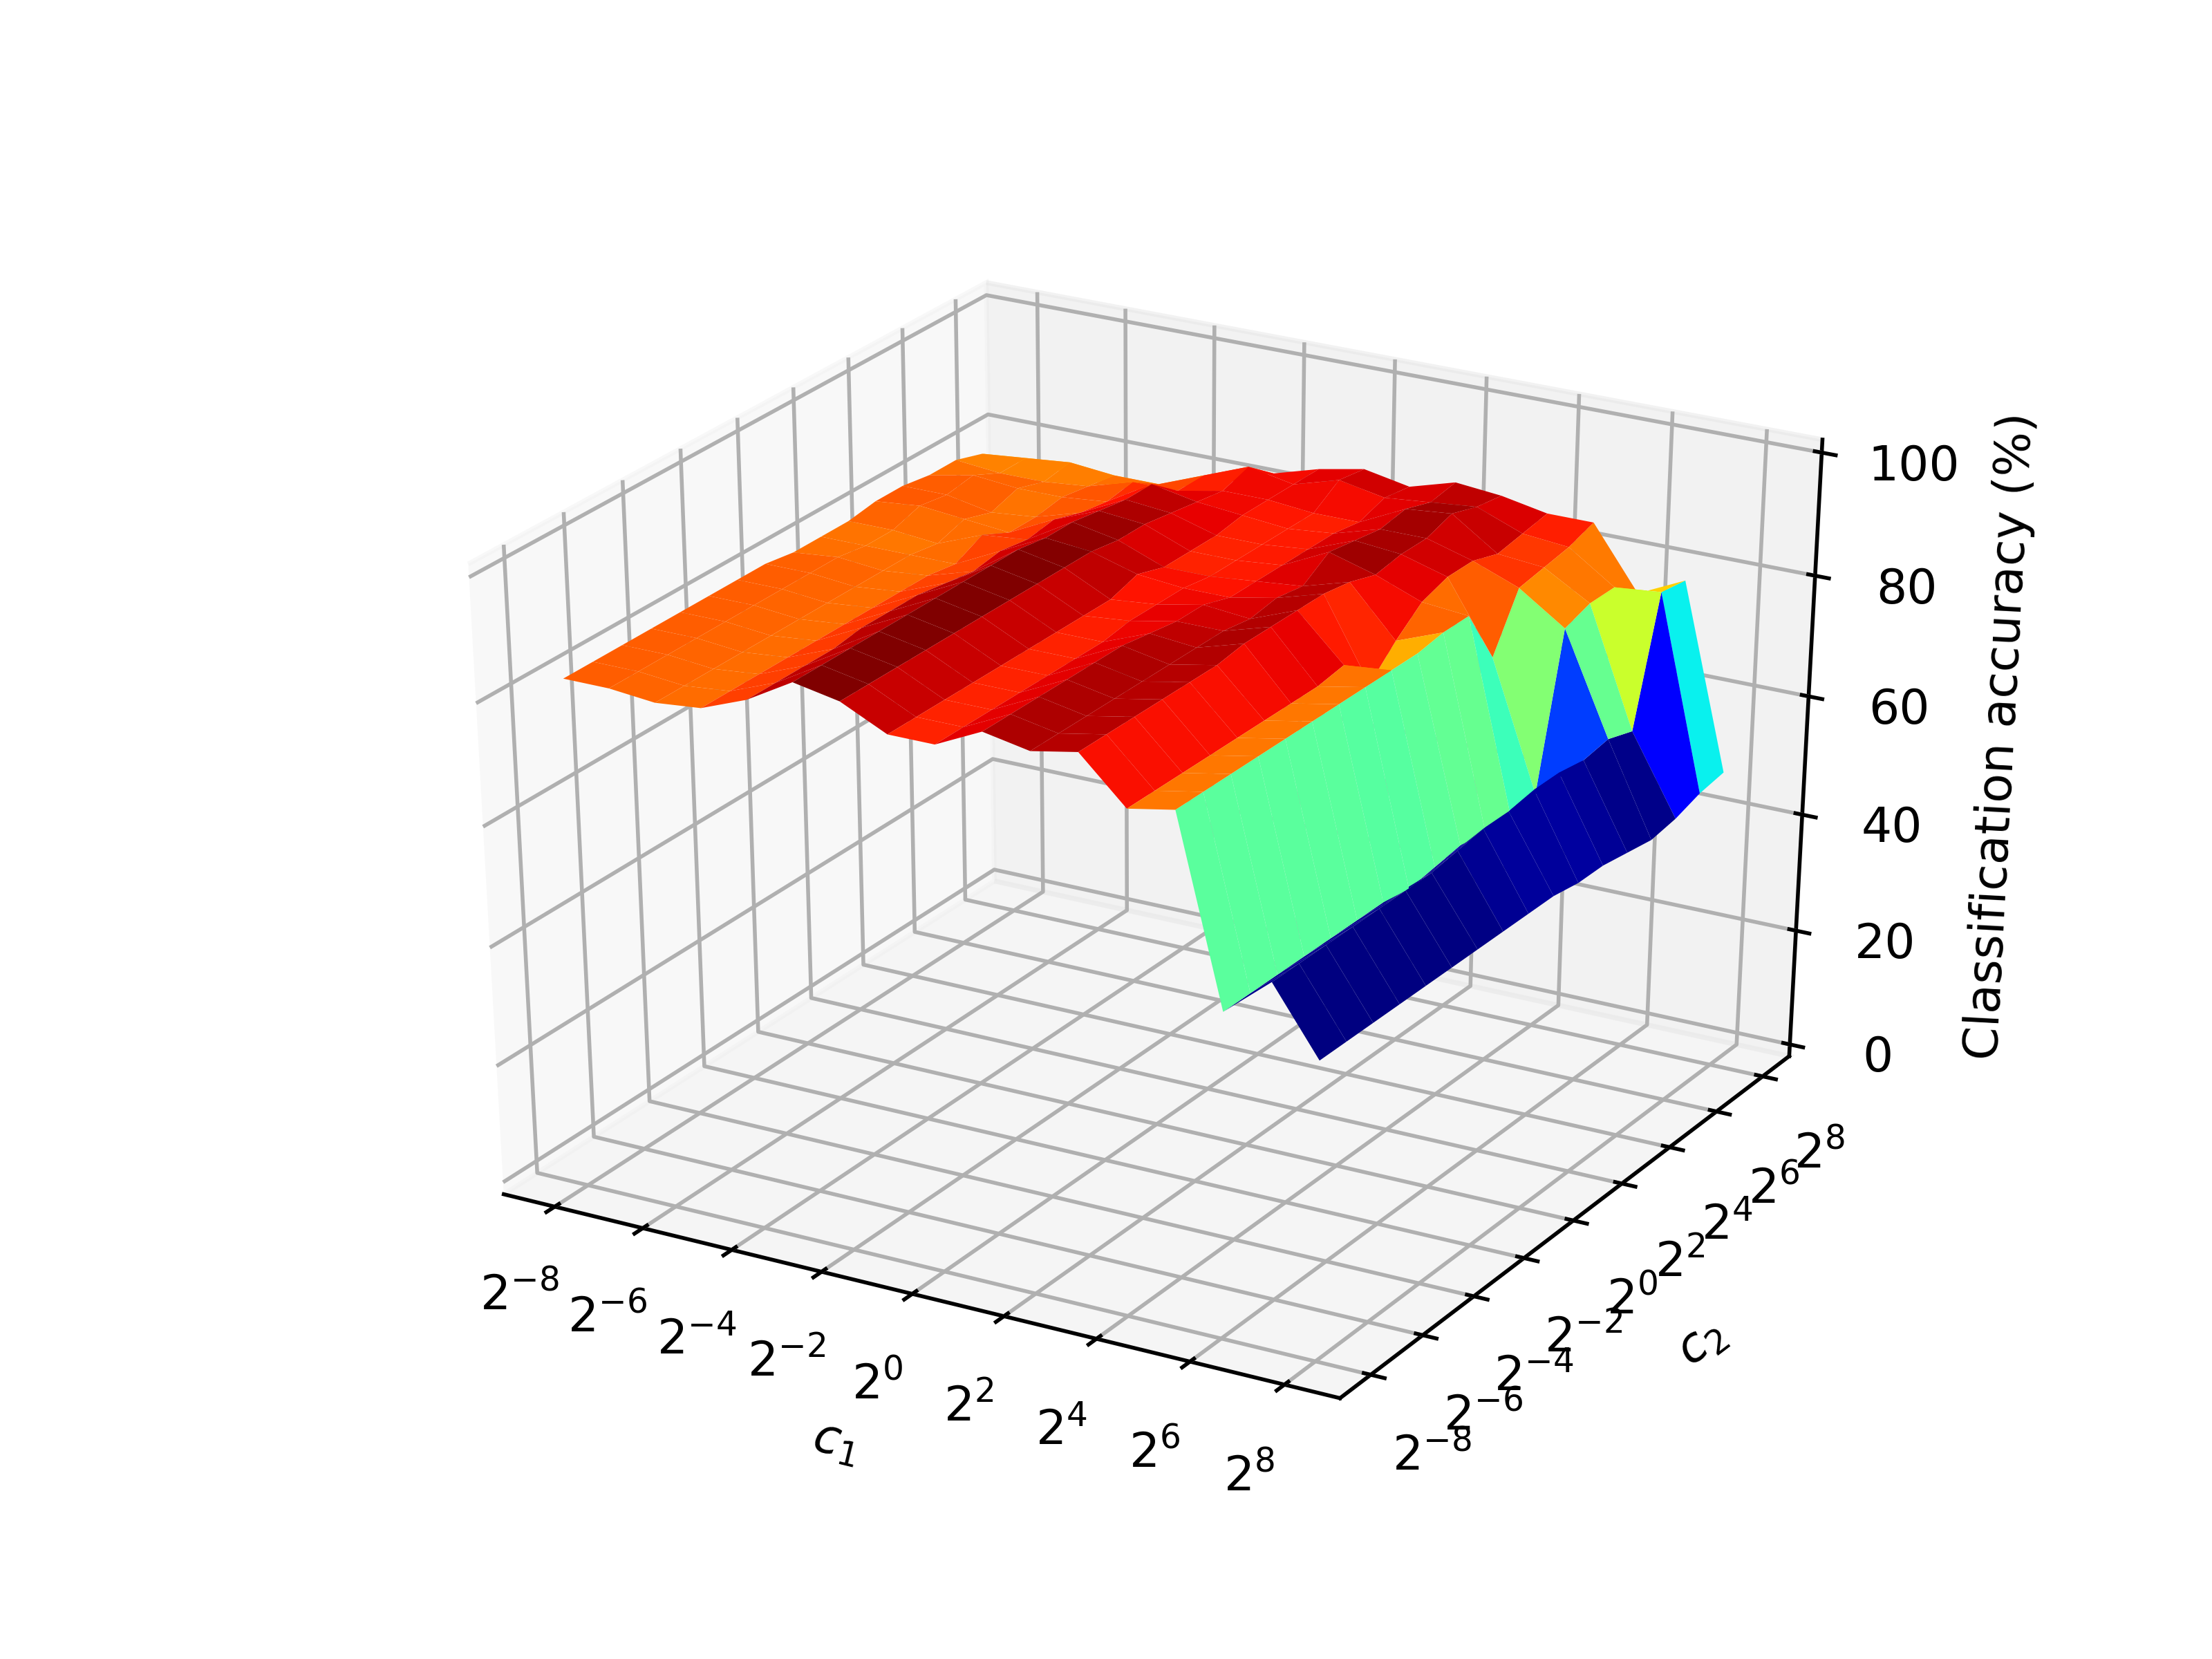
\includegraphics[width=0.5\textwidth]{RKNN-TSVM-Aust-C_1_2}}
	\subfloat[مجموعه داده \lr{Hepatitis}]{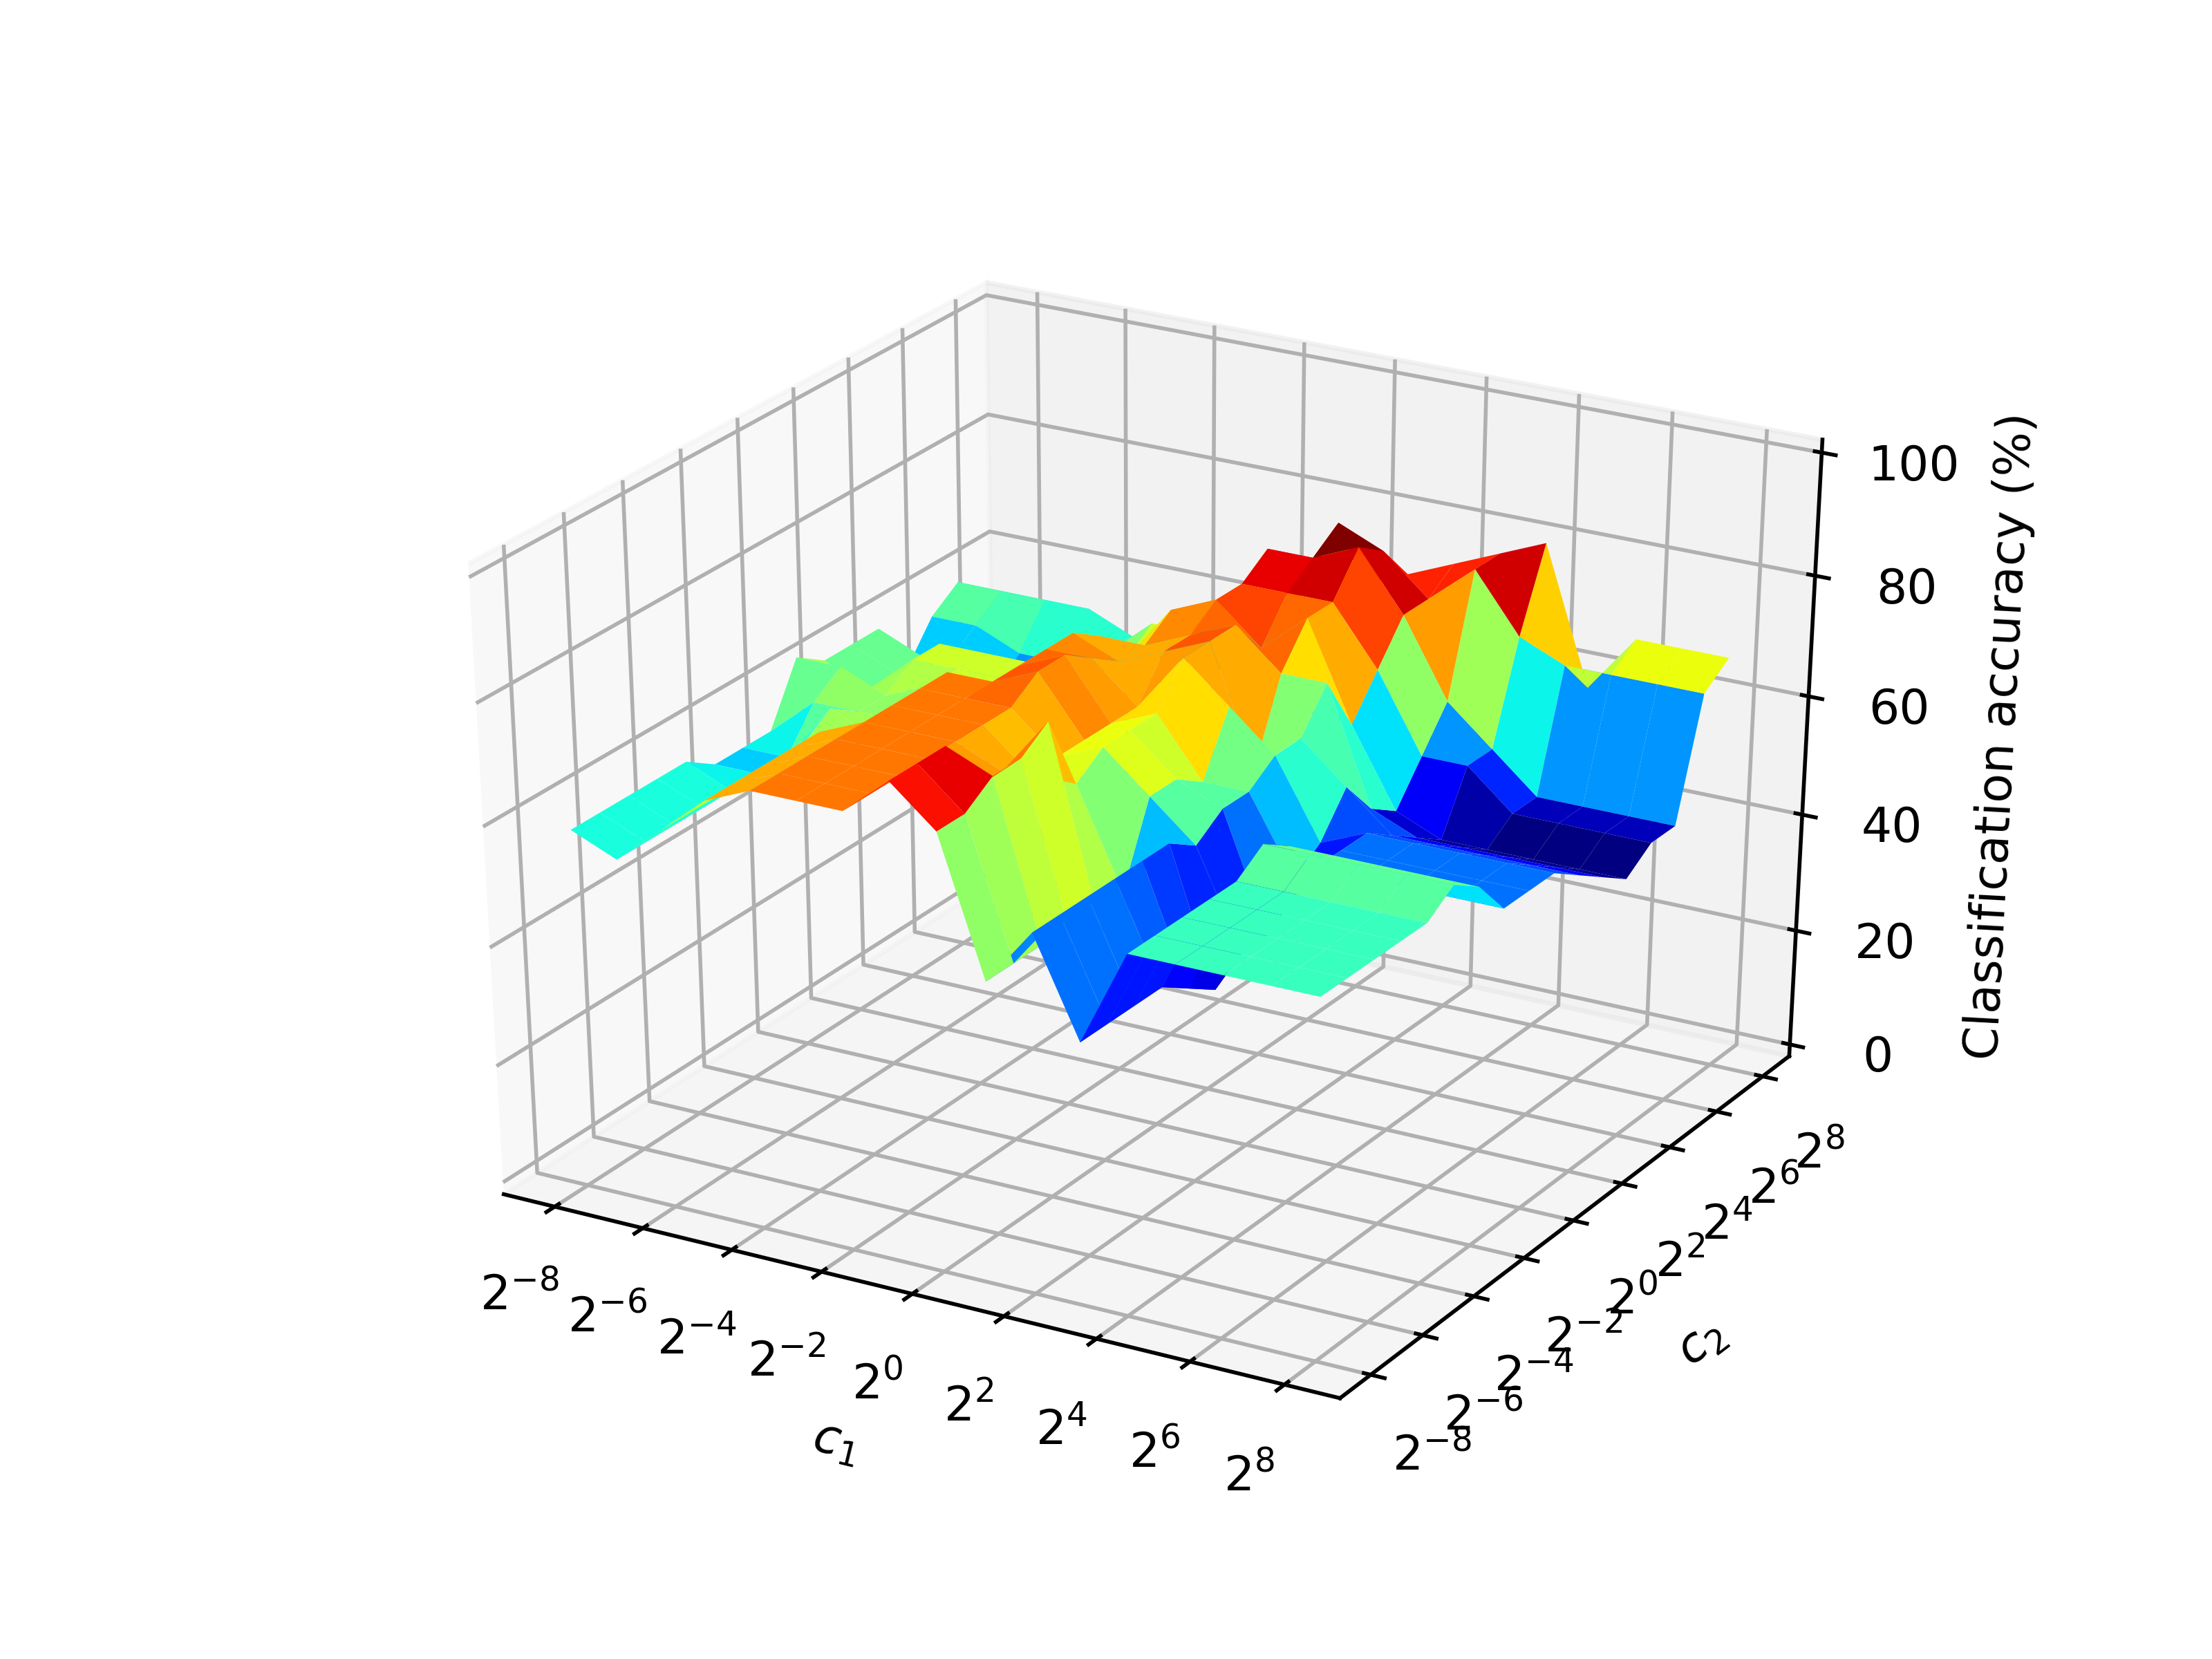
\includegraphics[width=0.5\textwidth]{RKNN-TSVM-Hep-C_1_2}}
	\caption{عملکرد نسخه خطی روش \lr{RKNN-TSVM} روی پارامترهای مختلف $c_{1}$ و $c_{2}$}
	\label{fig:RKNN-TSVM-Aust-Hep-C_1_2}
\end{figure}
\begin{figure}[!t]
	\centering
	\subfloat[مجموعه داده \lr{Australian}]{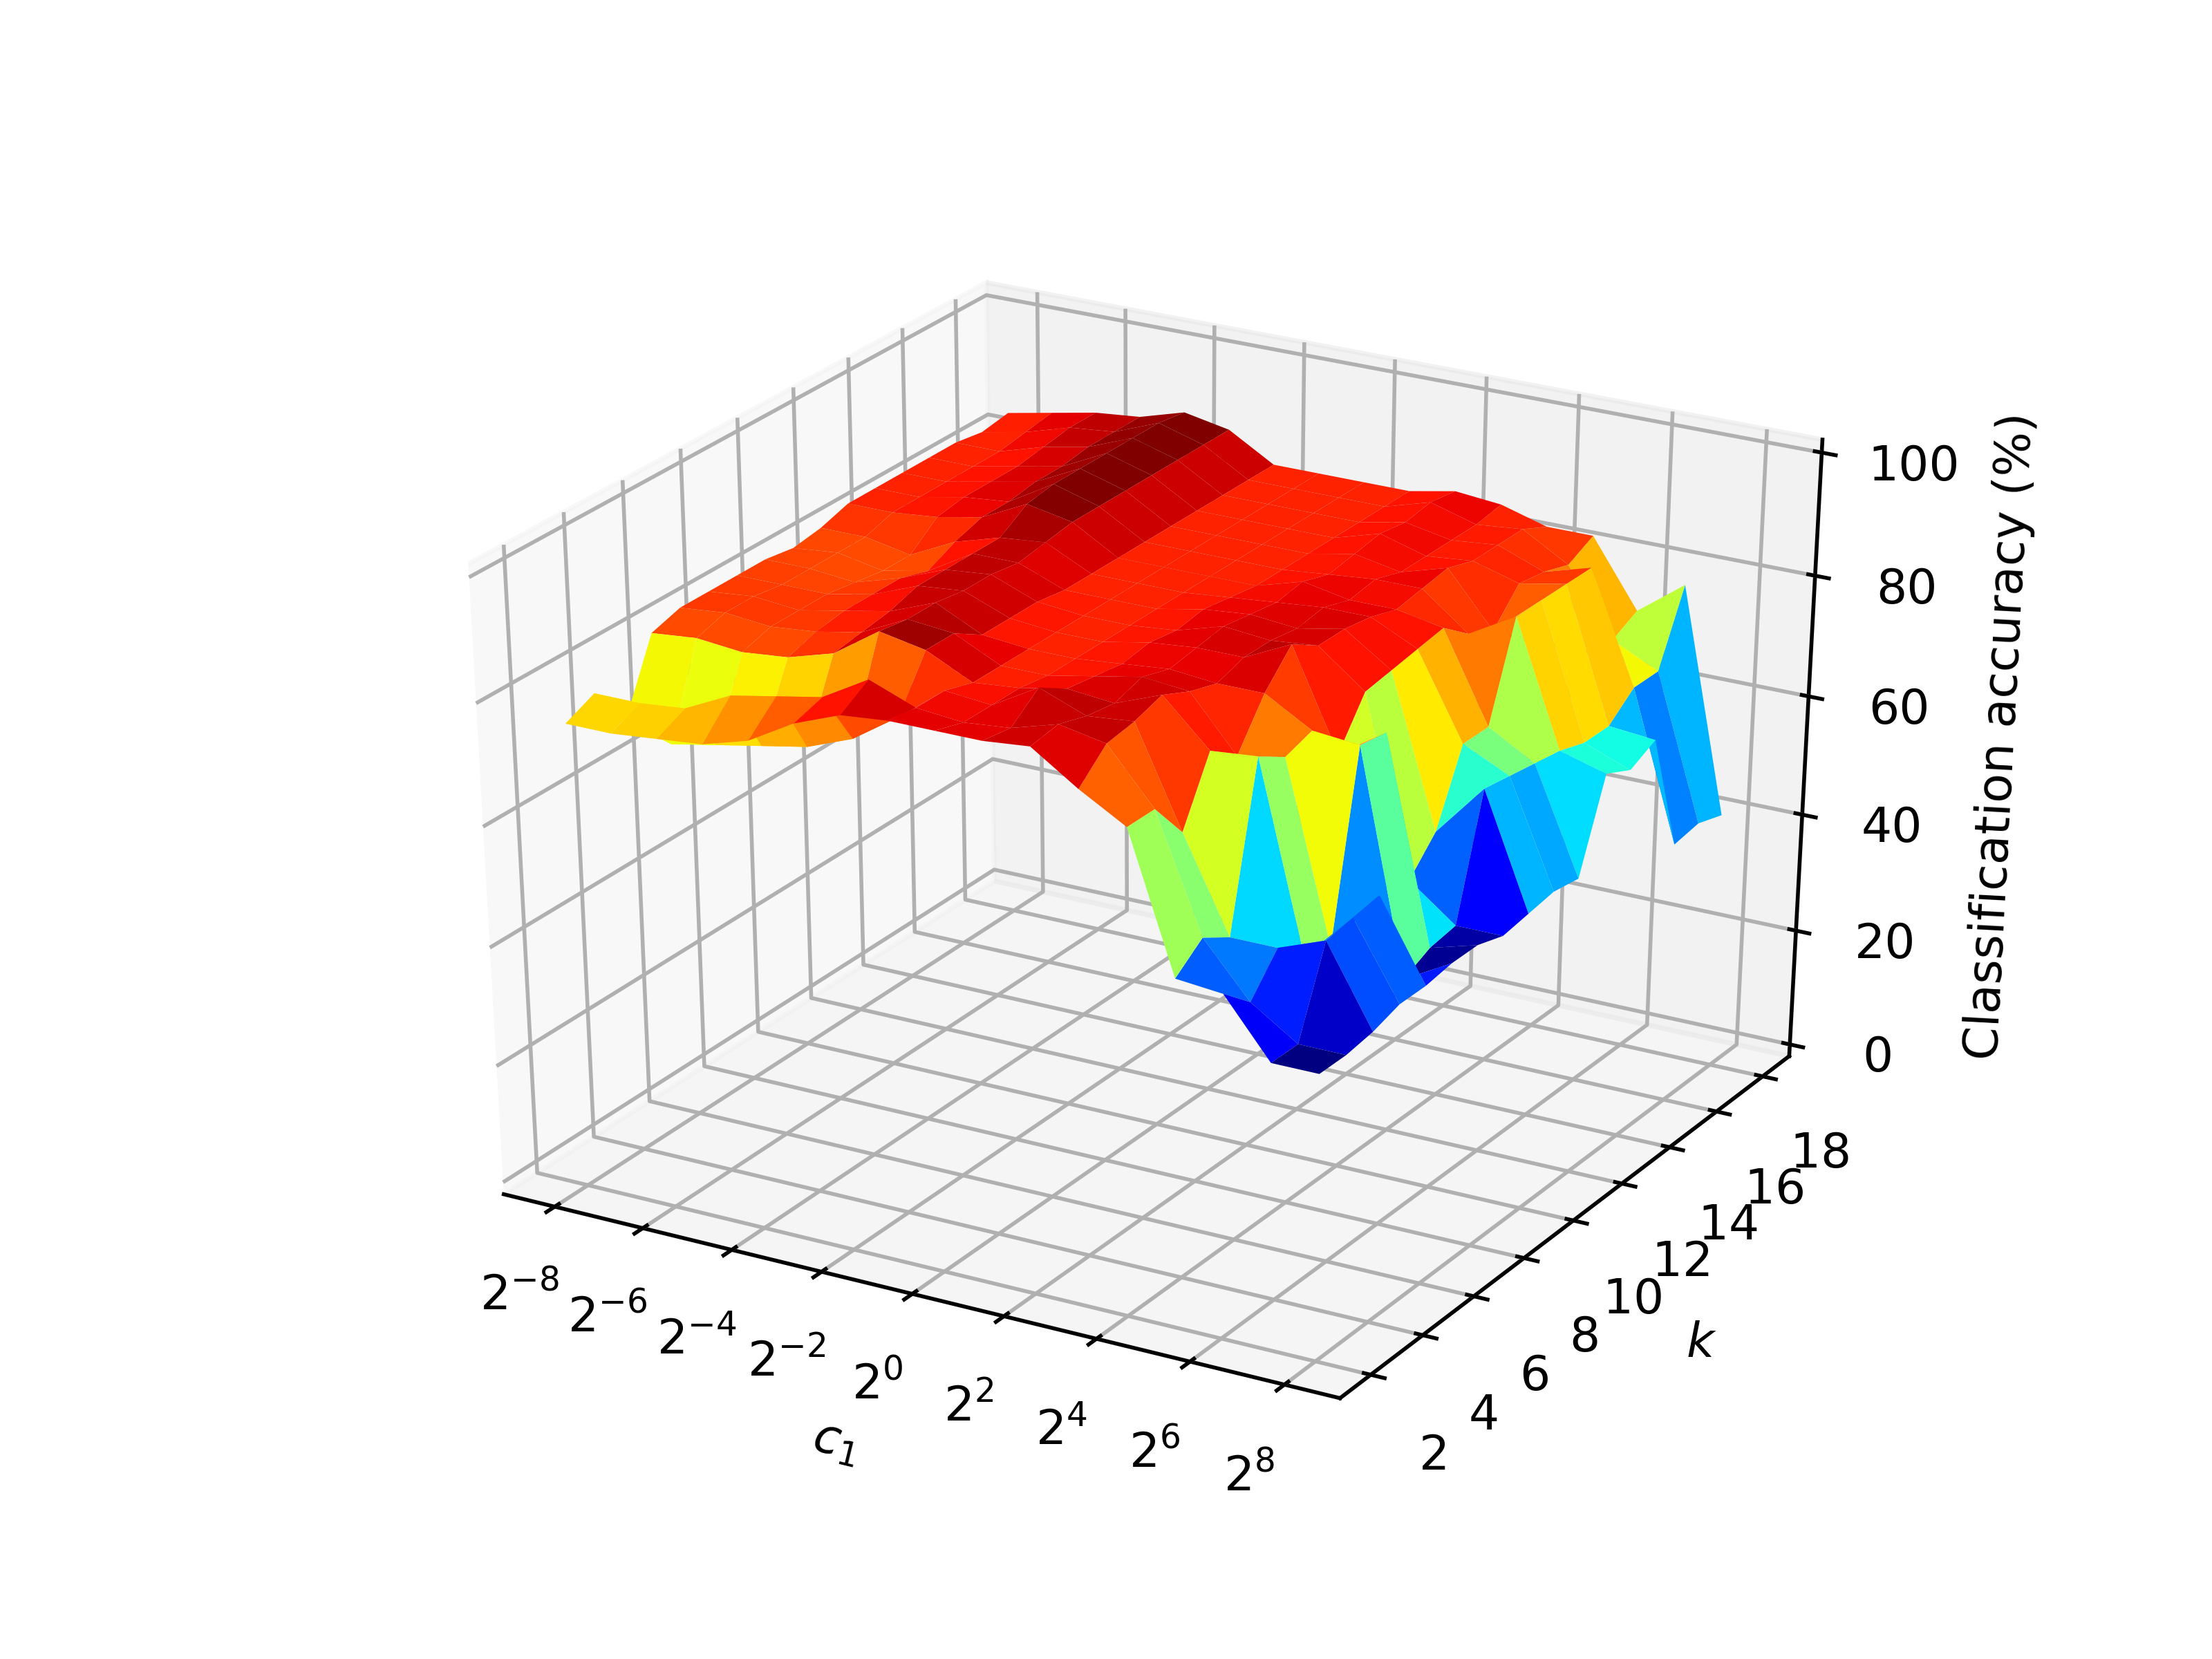
\includegraphics[width=0.5\textwidth]{RKNN-TSVM-Aust-C_1_k}}
	\subfloat[مجموعه داده \lr{Hepatitis}]{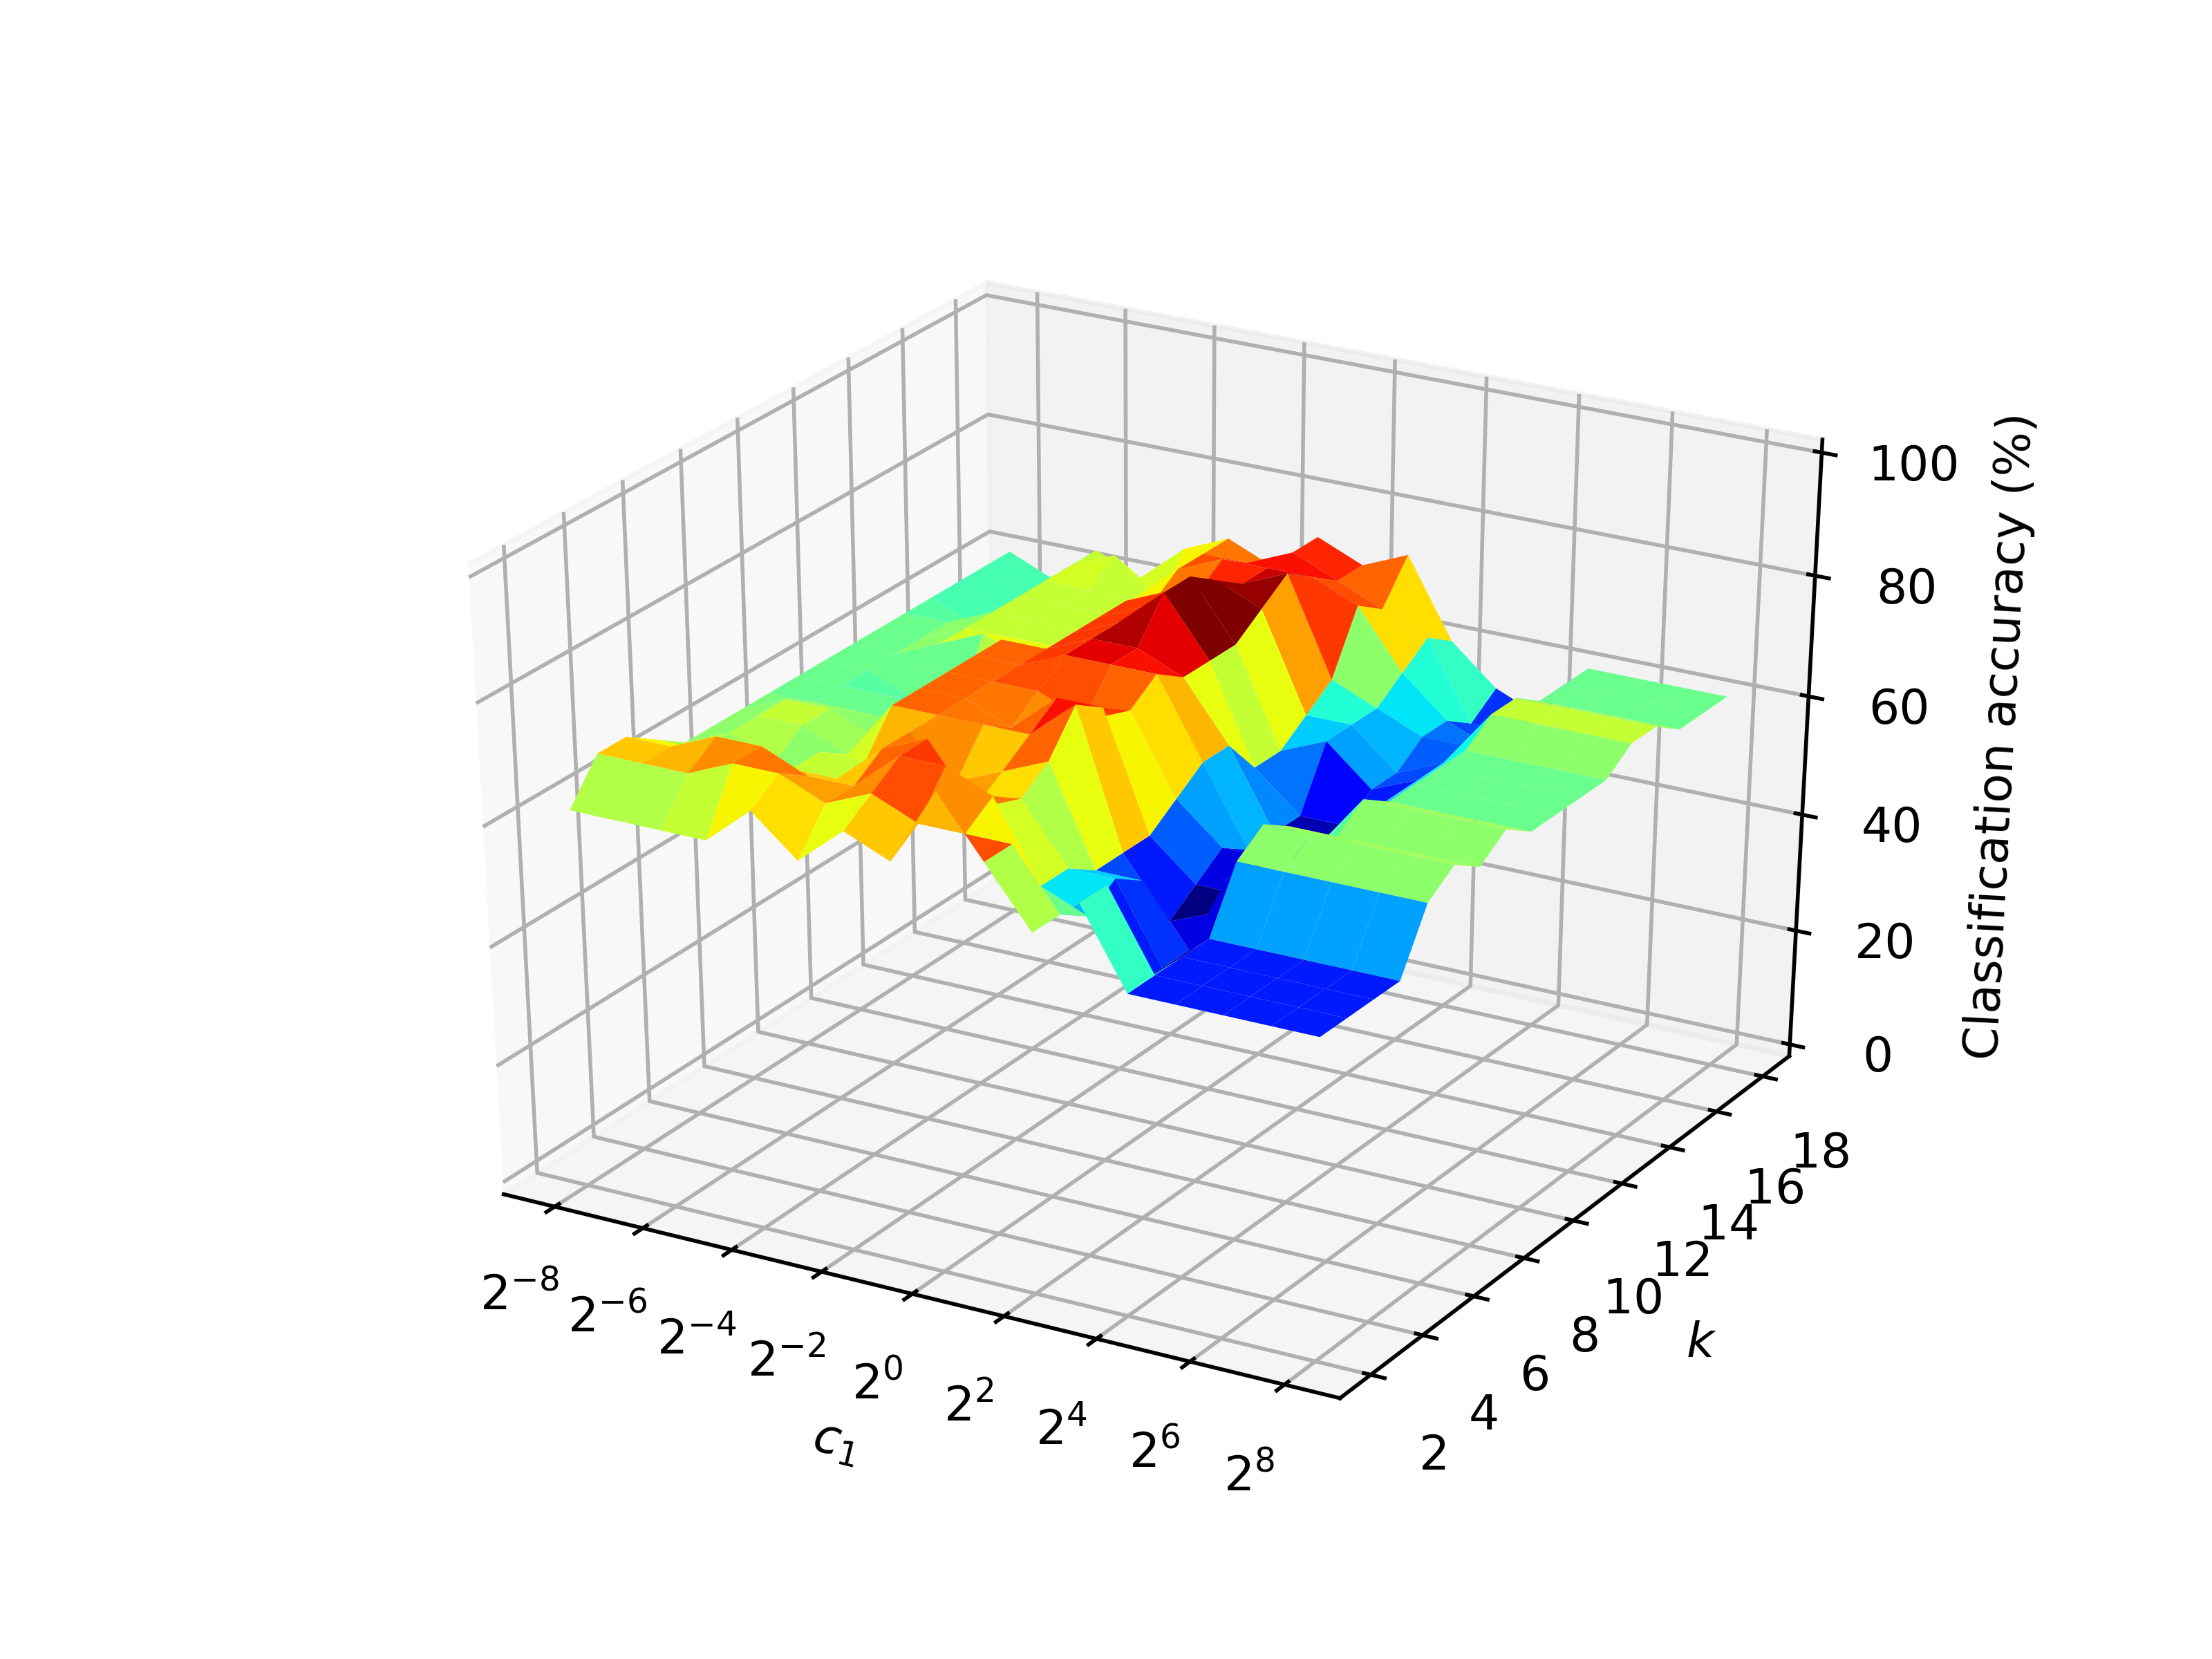
\includegraphics[width=0.5\textwidth]{RKNN-TSVM-Hep-C_1_k}}
	\caption{عملکرد نسخه خطی روش \lr{RKNN-TSVM} روی پارامترهای مختلف $c_{1}$ و $k$}
	\label{fig:RKNN-TSVM-Aust-Hep-C_1_k}
\end{figure}

برای هر مجموعه داده، در این آزمایش، تعداد حالت‌های پارامترهای $c_{1}$ $c_{2}$، و $k$ برابر با 17 است. بطوریکه تعداد ترکیبات $(c_{1},c_{2})$ و $(c_{1}, k)$ مساوی با 289 می‌باشد. شکل \ref{fig:RKNN-TSVM-Aust-Hep-C_1_2} عملکرد نسخه خطی روش روی پارامترهای مختلف $c_{1}$ و $c_{2}$ نشان می‌دهد. همانطور در این شکل نشان داده شده است، مقادیر پارامتر $c_{2}$ دقت دسته‌بندی روش \lr{RKNN-TSVM} را بهبود می‌دهد. بنابراین می‌توان نتیجه گرفت که ریسک ساختاری دقت روش ‍پیشنهادی (\lr{RKNN-TSVM}) را بهتر می‌کند.

شکل \ref{fig:RKNN-TSVM-Aust-Hep-C_1_k} عملکرد نسخه خطی روش \lr{RKNN-TSVM} روی مقادیر پارامترهای $c_{1}$ و $k$ را نشان می‌دهد. همانطور که در این شکل مشخص شده است، عملکرد روش \lr{RKNN-TSVM} به پارامتر $k$ نیز وابسته است. به عنوان مثال، افزایش مقدار پارامتر $k$ منجر به بهبود دقت روش پیشنهادی روی مجموعه داده \lr{Hepatitis} شده است. به طور خلاصه، آزمایش‌های این بخش نشان می‌دهد که دقت روش پیشنهادی (\lr{RKNN-TSVM}) وابسته به انتخاب بهینه پارامترهایش است.

\subsubsection{آزمایش با مجموعه داده \lr{NDC}}\label{sec:5:3:3:5}
به منظور بررسی سرعت آموزش روش \lr{RKNN-TSVM} بر روی مجموعه داده‌های بزرگ، آزمایش بر روی مجموعه داده \lr{NDC} \cite{musicant1998} صورت گرفته است. مشخصات مجموعه داده‌های \lr{NDC} در جدول \ref{tab:5} نشان داده شده است. جهت آزمایش با مجموعه داده \lr{NDC}، پارامتر $C$ برای تمام روش برابر با یک است. در نسخه غیر خطی از تابع \lr{RBF} با پارامتر $\sigma=2^{-15}$ استفاده شده است. همچنین پارامتر  $k$ برای روش‌های \lr{WLTSVM} و \lr{RKNN-TSVM} برابر با 5 است. 

جدول \ref{tab:11} مقایسه زمان آموزش روش‌های \lr{TSVM}،\lr{WLTSVM} و \lr{RKNN-TSVM} با تابع هسته خطی را نشان می‌دهد. مشابه روش \lr{TSVM}، روش \lr{TBSVM} دو مسئله دوگان را برای بدست آوردن مدل خروجی حل می‌کند. بنابراین زمان آموزش روش \lr{TBSVM} در این آزمایش آورده نشده است. ستون آخر نسبت تسریع الگوریتم \lr{LDMDBA} را نشان می‌دهد که به این صورت تعریف می‌شود: 
\begin{align*}
%\small
\textrm{نسبت تسریع} = \frac{\textrm{زمان آموزش روش \lr{RKNN-TSVM(FSA)}}}{\textrm{زمان آموزش روش \lr{RKNN-TSVM(LDMDBA)}}}
\end{align*}

نتایج در جدول \ref{tab:11} نشان می‌دهد که الگوریتم \lr{LDMDBA} سرعت آموزش روش پیشنهادی را به طور قابل توجه‌ای بهبود داده است. بطوریکه با افزایش تعداد نمونه‌های آموزشی، نسبت تسریع الگوریتم \lr{LDMDBA} بیشتر می‌شود. برای مثال، روش پیشنهادی با الگوریتم \lr{LDMDBA} از روش پیشنهادی با الگوریتم \lr{FSA} روی مجموعه داده \lr{NDC-25K} حدود $3.25$ سریع‌تر است. همچنین سرعت آموزش نسخه خطی روش \lr{RKNN-TSVM} با الگوریتم \lr{LDMDBA} بسیار نزدیک به نسخه خطی \lr{TSVM} می‌باشد. بطوریکه نسخه خطی روش پیشنهادی از  نسخه خطی \lr{TSVM} روی مجموعه داده \lr{NDC-50K} کمی سریع‌تر است. زیرا روش پیشنهادی دو مسئله دوگان با اندازه کوچک‌تر حل می‌کند. به عبارت دیگر فقط نمونه‌های حاشیه‌ای در مسئله دوگان نقش دارند.

\begin{table*}[!t]
	\small
	\centering
	\caption{مقایسه زمان آموزش روش \lr{RKNN-TSVM} با سایر روش روی مجموعه داده \lr{NDC} با تابع هسته خطی}
	\ra{1.3} % Space between rows
	\begin{threeparttable}
		\begin{tabular}{l c c c c c}
			\toprule
			% after \\: \hline or \cline{col1-col2} \cline{col3-col4} ...
			مجموعه داده & \lr{TSVM} & \lr{WLTSVM} & \lr{RKNN-TSVM(FSA)} & \lr{RKNN-TSVM(LDMDBA)} & \\
			& زمان اجرا & زمان اجرا & زمان اجرا & زمان اجرا  & نسبت تسریع \\
			\midrule
			%NDC-700 & 0.019 & 0.047 & 0.042 & 0.032 & 1.31\\ 
			%NDC-900 & 0.031 & 0.079 & 0.065 & 0.042 & 1.55\\ 
			\lr{NDC-1K} & $0.064$ & $0.092$ & $0.079$ & $0.052$ & $1.52$\\ 
			\lr{NDC-2K} & $0.12$ & $0.36$ & $0.292$ & $0.19$ & $1.54$\\ 
			\lr{NDC-3K} & $0.26$ & $0.84$ & $0.662$ & $0.295$ & $2.24$\\ 
			\lr{NDC-4K} & $0.422$ & $1.476$ & $1.192$ & $0.562$ & $2.12$ \\
			\lr{NDC-5K} & $0.693$ & $2.397$ & $1.884$ & $0.828$ & $2.28$\\
			\lr{NDC-10K} & $2.556$ & $9.872$ & $7.628$ & $2.727$  & $2.8$ \\
			\lr{NDC-25K} & $17.606$ & $68.893$ & $52.867$ & $16.25$  & $3.25$\\
			\lr{NDC-50K} & $70.1$ & \tnote{\lr{a}} & \tnote{\lr{a}} & $64.433$  & -\\
			\bottomrule
		\end{tabular}
		\begin{tablenotes}
			\item[\lr{a}] آزمایش به دلیل کمبود حافظه خاتمه یافته است.
		\end{tablenotes}
	\end{threeparttable}
	\label{tab:11}
\end{table*}

\begin{table*}[!t]
	\small
	\centering
\caption{مقایسه زمان آموزش روش \lr{RKNN-TSVM} با سایر روش روی مجموعه داده \lr{NDC} با تابع هسته \lr{RBF}}
	\ra{1.3} % Space between rows
	\begin{threeparttable}
		\begin{tabular}{l c c c c c}
			\toprule
			% after \\: \hline or \cline{col1-col2} \cline{col3-col4} ...
			مجموعه داده & \lr{TSVM} & \lr{WLTSVM} & \lr{RKNN-TSVM(FSA)} & \lr{RKNN-TSVM(LDMDBA)} & \\
			& زمان اجرا & زمان اجرا & زمان اجرا & زمان اجرا  & نسبت تسریع\\
			\midrule
			%NDC-700 & 0.102 & 0.315 & 0.309 & 0.273 & 1.13 \\ 
			%NDC-900 & 0.161 & 0.611 & 0.591 & 0.454 & 1.3 \\ 
			\lr{NDC-1K} & $0.203$ & $0.803$ & $0.807$ & $0.555$ & $1.45$\\ 
			\lr{NDC-2K} & $0.983$ & $5.731$ & $5.729$ & $2.442$ & $2.35$\\ 
			\lr{NDC-3K} & $2.74$ & $18.225$ & $18.599$ & $6.465$ & $2.88$\\
			\lr{NDC-4K} & $5.896$ & $42.234$ & $41.784$ & $12.485$ & $3.35$\\ 
			\lr{NDC-5K} & $10.328$ & $84.188$ & $82.507$ & $21.14$ & $3.9$\\
			\lr{NDC-10K}\textsuperscript{\lr{b}} & $4.605$ & $67.626$ & $64.721$ & $8.606$ & $7.52$\\
			\lr{NDC-25K}\textsuperscript{\lr{b}} & $31.459$ & $983.678$ & $963.341$ & $67.485$  & $14.27$\\
			\lr{NDC-50K}\textsuperscript{\lr{b}} & $186.761$ & \tnote{\lr{a}} & \tnote{\lr{a}} & $357.942$  & -\\
			\bottomrule
		\end{tabular}
		\begin{tablenotes}
			\item[\lr{a}]  اجرای روش به دلیل زیاد بودن زمان آزمایش خاتمه یافته است.
			\item[\lr{b}] از تابع هسته مستطیلی با اندازه 10 درصد نمونه‌های آموزشی استفاده شده است.
		\end{tablenotes}
	\end{threeparttable}
	\label{tab:12}
\end{table*}

جدول \ref{tab:12} مقایسه زمان آموزش روش‌های \lr{TSVM}،\lr{WLTSVM} و \lr{RKNN-TSVM} با تابع هسته \lr{RBF} را نشان می‌دهد. نتایج با تابع هسته غیر خطی نشان می‌دهد که روش پیشنهادی با الگوریتم \lr{LDMDBA} از روش \lr{WLTSVM}  و روش \lr{RKNN-TSVM} با الگوریتم  \lr{FSA} بسیار سریع‌تر است. بطوریکه بیشترین نسبت تسریع با الگوریتم \lr{LDMDBA} مساوی با 14 برابر می‌باشد. با وجود اینکه از تابع هسته تقلیل یافته برای مجموعه داده‌های بزرگ از 5 هزار نمونه استفاده شده است،  روش \lr{TSVM} همچنان حدود 2 برابر سریع‌تر از روش پیشنهادی با الگوریتم \lr{LDMDBA} است. زیرا روش پیشنهادی با الگوریتم \lr{LDMDBA} و تابع هسته تقلیل یافته $(n \times \bar{n})$ علاوه بر پیدا کردن نزدیک‌ترین همسایه‌های تمام نمونه‌ها، دو مسئله دوگان نیز حل می‌کند.

نتایج روی مجموعه داده \lr{NDC} با تابع هسته \lr{RBF} این فرضیه را تایید می‌کند که الگوریتم \lr{LDMDBA} برای نسخه غیر خطی روش  \lr{RKNN-TSVM} مناسب است. زمان اجرای این الگوریتم روی داده‌های با ابعاد بالا بسیار بهتر از الگوریتم \lr{FSA} می‌باشد. به طور خلاصه، روش \lr{RKNN-TSVM} با الگوریتم \lr{LDMDBA} نسبت به روش \lr{WLTSVM} روی مجموعه داده‌های بزرگ از نظر زمان اجرا بسیار بهتر عمل می‌کند.

\section{جمع‌بندی}\label{sec:5:4}
در این فصل، دو دسته‌بند پیشنهادی یعنی \lr{KNN-LSTSVM} و \lr{RKNN-TSVM} مورد بررسی و ارزیابی قرار گرفت. روش \lr{KNN-LSTSVM} مزیت‌های اصلی دو روش \lr{WLTSVM} و \lr{LSTSVM} را دارد که عبارتند از:
\begin{enumerate}
	\item مشابه روش \lr{WLTSVM}، اطلاعات شباهت نمونه‌ها را با ساخت گراف نزدیک‌ترین همسایه در مسئله بهینه‌سازی لحاظ می‌کند. بطوریکه به هر نمونه بر اساس شمارش تعداد همسایه‌های نزدیکش وزن داده می‌شود. همچنین نمونه‌های حاشیه‌ای هر کلاس نیز با استفاده از گراف ساخته شده مشخص می‌گردد.  نتایج بر روی مجموعه داده‌های مصنوعی (بخش \ref{sec:5:2:2}) و واقعی (بخش \ref{sec:5:2:3}) نشان می‌دهد دقت مدل خروجی نسبت به روش \lr{LSTSVM} بهبود یافته است .
	\item مشابه روش \lr{LSTSVM}، قید مسئله بهینه‌سازی در تابع هدف جایگذاری می‌شود. بطوریکه مدل خروجی با حل کردن دو دستگاه معادلات خطی بدست می‌آید. در حالی‌که در روش  \lr{WLTSVM} دو مسئله دوگان حل می‌شود. نتایج ارزیابی روی مجموعه داده‌های بزرگ  (بخش \ref{sec:5:2:4}) نشان می‌دهد که سرعت آموزش نسبت به روش \lr{WLTSVM} بسیار افزایش یافته است.    
\end{enumerate}

روش پیشنهادی دوم یعنی \lr{RKNN-TSVM} روش \lr{WLTSVM} را از نظر دقت و سرعت آموزش بهبود داده است:
\begin{enumerate}
	\itemsep0em
	\item \lr{RKNN-TSVM} برخلاف روش  \lr{WLTSVM} به یک نمونه براساس فاصله نزدیک‌ترین همسایه‌هایش از نمونه مورد نظر وزن می‌دهد. همچنین روش پیشنهادی ریسک ساختاری را در مسئله بهینه سازی کمینه می‌کند. نتایج بر روی مجموعه داده‌های مصنوعی  (بخش \ref{sec:5:3:3:1}) و واقعی (بخش  \ref{sec:5:3:3:2}) نشان می‌دهد که دقت دسته‌بندی و تعمیم‌پذیری روش پیشنهادی نسبت به روش \lr{WLTSVM} بهبود یافته است.
	\item محاسبه گراف نزدیک‌ترین همسایه جهت وزن‌دهی به نمونه‌ها، یک چالش در روش پیشنهادی است. به منظور حل کردن این چالش، الگوریتم  \lr{LDMDBA} به منظور سرعت بخشیدن به فرآیند پیدا کردن نزدیک‌ترین همسایه‌های نمونه‌ها استفاده شده است. نتایج بر روی مجموعه داده‌های بزرگ نشان می‌دهد که الگوریتم  \lr{LDMDBA} سرعت آموزش روش پیشنهادی را برای هر دو نسخه خطی و غیر خطی به طور قابل    توجه‌ای افزایش داده است. بطوریکه سرعت یادگیری تا 14 برابر نسبت به روش \lr{WLTSVM} سریع‌تر شده است.
\end{enumerate}



% Conclusion

\chapter{نتیجه‌گیری و پژوهش‌های آینده}\label{ch:6}

\section{مقدمه}\label{sec:6:1}
در این فصل، ابتدا ویژگی‌های دسته‌بندهای پیشنهادی مرور می‌شود. سپس یافته‌های مهم این پژوهش به طور خلاصه بیان می‌شود. در آخر، پیشنهاد هایی برای پژوهش‌های آینده بیان می‌گردد.

\section{مروری بر دسته‌بندهای پیشنهادی}\label{sec:6:2}
هدف اصلی این پژوهش، ارائه یک دسته‌بند مبتنی بر ماشین بردار پشتیبان دو قلو است که بتواند دقت و تعمیم‌پذیری مطلوبی در برابر داده‌های نویزی و پرت داشته باشد. بدین منظور دو دسته‌بند \lr{KNN-LSTSVM} و \lr{RKNN-TSVM} به ترتیب در فصول \ref{ch:3} و \ref{ch:4} ارائه شد.

دسته‌بند \lr{KNN-LSTSVM} \cite{mir2018} با ایده گرفتن از روش \lr{WLTSVM} گراف نزدیک‌ترین همسایه را برای تمام نمونه‌های آموزشی ایجاد می‌کند. سپس با استفاده از گراف درون کلاسی $W_{w}$ به نمونه‌ها بر اساس شماری تعداد همسایه‌های نزدیک‌شان وزن می‌دهد و همچنین با بکارگیری گراف برون کلاسی $W_{b}$، نمونه‌های حاشیه‌ای هر کلاس را مشخص می‌کند. بطوریکه دقت و تعمیم‌پذیری روش \lr{KNN-LSTSVM} نسبت به روش \lr{TSVM} با وجود داده‌های نویزی بهتر است. به منظور افزایش سرعت یادگیری و آموزش، روش \lr{KNN-LSTSVM} همانند روش \lr{LSTSVM} قید مسئله بهینه‌سازی را در تابع هدف جایگذاری می‌کند. بطوریکه مدل خروجی با حل کردن دو دستگاه معادلات خطی بدست می‌آید. دسته‌بند پیشنهادی در بخش \ref{sec:5:2} مورد ارزیابی و بررسی قرار گرفت. نتایج نشان می‌دهد که روش پیشنهادی نسبت به روش \lr{TSVM} از نظر دقت دسته‌بندی و سرعت یادگیری به طور قابل توجه‌ای بهتر می‌باشد.

در ادامه، دسته‌بند \lr{RKNN-TSVM} با هدف برطرف کردن مشکلات روش \lr{WLTSVM} ارائه شده است. روش پیشنهادی  سه مزیت نسبت به روش  \lr{WLTSVM} دارد که عبارتند از:
\begin{enumerate}
	\item روش پیشنهادی به نمونه‌ها بر اساس فاصله از نزدیک‌ترین همسایه‌شان وزن می‌دهد. برای مثال، اگر  فاصله نزدیکترین همسایه‌های یک نمونه از آن بسیار کم باشد، وزن بیشتری به این نمونه نسبت داده می‌شود. این شیوه وزن‌دهی نمونه‌های پرتراکم را بهتر  از روش  \lr{WLTSVM}شناسایی می‌کند.
	\item روش پیشنهادی \lr{RKNN-TSVM} برخلاف روش \lr{WLTSVM} ریسک ساختاری را کمینه می‌کند. زیرا جمله رگولارسیون به مسائل بهینه‌سازی روش پیشنهادی اضافه شده است. بطوریکه مانند روش  \lr{SVM} حاشیه بیشینه می‌گردد. کمینه کردن ریسک ساختاری در روش پیشنهادی باعث بهبود تعمیم‌پذیری آن شده است.
	\item سرعت یادگیری روش  \lr{WLTSVM}به دلیل محاسبه گراف نزدیک‌ترین همسایه برای مجموعه داده‌های بزرگ بسیار کاهش می‌یابد. با  این حال روش پیشنهادی از الگوریتم \lr{LDMDBA} برای ساخت گراف نزدیک‌ترین همسایه استفاده می‌کند. مرتبه زمانی این الگوریتم برابر با   $\mathcal{O}(\log nm\log m)$ است. بطوریکه سرعت یادگیری روش پیشنهادی نسبت به روش \lr{WLTSVM} برای مجموعه داده‌های بزرگ به طور قابل    توجه‌ای سریعتر است. 
\end{enumerate} 

نتایج بدست آمده در بخش \ref{sec:5:3}، مزیت‌های دسته‌بند \lr{RKNN-TSVM} نسبت به روش \lr{WLTSVM} را تایید می‌کند.

\section{مروری بر یافته‌های این پژوهش}\label{sec:6:3}
در فصل \ref{ch:5}، دو دسته‌بند پیشنهادی یعنی \lr{KNN-LSTSVM} و \lr{RKNN-TSVM} به طور جامع بررسی و ارزیابی شده است. در این بخش یافته‌های مهم و اصلی این پژوهش براساس نتایج ارزیابی به طور خلاصه در زیر بیان شده است.
\begin{itemize}[label=$\bullet$]
	\item روش‌های  \lr{KNN-LSTSVM} و  \lr{WLTSVM} با در نظر گرفتن گراف درون کلاسی در مسئله بهینه‌سازی‌شان به نمونه‌های آموزشی وزن می‌دهند. بطوریکه مدل خروجی نسبت به نمونه‌های پرت و نویزی حساسیت کمتری خواهد داشت. در نتیجه دقت و تعمیم‌پذیری مدل خروجی افزایش می‌یابد.
	\item روش‌های  \lr{LSTSVM} و  \lr{KNN-LSTSVM} با استفاده از تکنیک کمترین مربعات، قید مسئله بهینه‌سازی را در تابع هدف جایگذاری می‌کنند. بدین ترتیب مدل خروجی با حل کردن دو دستگاه معادلات خطی بدست می‌آید. فرآیند یادگیری در این گونه روش‌ها برای مجموعه داده‌های بزرگ بسیار سریع است.
	\item روش‌های \lr{WLTSVM} و  \lr{RKNN-TSVM} با در نظر گرفتن گراف برون کلاسی در مسائل بهینه‌سازی‌شان، نمونه‌های حاشیه‌ای هر کلاس را مشخص می‌کنند. بطوریکه ابرصفحه به جای تمام نمونه‌های کلاس مقابل، فقط از نمونه‌های حاشیها‌‌‌ی کلاس مقابل حداکثر فاصله ممکن را می‌گیرد. در نتیجه ابعاد مسئله بهینه‌سازی دوگان کوچکتر می‌شود. در نتیجه مرتبه زمانی دسته‌بند بهبود می‌یابد.
	\item روش پیشنهادی  \lr{RKNN-TSVM} همانند روش  \lr{TBSVM} ریسک ساختاری را کمینه می‌کند. بطوریکه مسائل بهینه‌سازی در این  روش‌ها مثبت معین است و از شرایط ماتریس منفرد جلوگیری شده است. با این حال کمینه کردن ریسک ساختاری منجر به معرفی یک پارامتر جدید به دسته‌بند می‌شود. از طرفی تنظیم کردن این پارامتر تعمیم‌پذیری مدل خروجی را بهبود داده است. از طرف دیگر، معرفی این پارامتر باعث افزایش بار محاسباتی جستجوی پارامترهای بهینه می‌شود. 
	\item روش  \lr{WLTSVM} براساس شمارش تعداد همسایه‌های نزدیک به یک نمونه وزن می‌دهد. در حالی‌که روش پیشنهادی  \lr{RKNN-TSVM} به یک نمونه براساس فاصله بین آن نمونه و نزدیک‌ترین همسایه‌هایش وزن می‌دهد. بطوریکه ماتریس وزن شامل اعداد بین بازه   $\left[0,1\right]$ است. این نوع شیوه وزن‌دهی باعث شناسایی بهتر نمونه‌های پرتراکم در فضای ویژگی می‌شود و همچنین نمونه‌های پرت و نویزی بهتر از روش \lr{WLTSVM} مشخص می‌شوند. نتایج نشان داده است که این نوع شیوه وزن‌دهی دقت دسته‌بند  را بهبود می‌دهد.
	\item با وجود اینکه روش پیشنهادی   \lr{RKNN-TSVM}با در نظر گرفتن نمونه‌های حاشیه‌ای، دو مسئله دوگان با ابعاد کوچک‌تر را حل می‌کند. محاسبه گراف نزدیک‌ترین همسایه سرعت یادگیری روش پیشنهادی را به طور قابل توجه‌ای کاهش می‌دهد. الگوریتم  \lr{LDMDBA}به منظور بهبود سرعت فرآیند ساخت گراف نزدیک‌ترین همسایه بکار گرفته شده است. نتایج آزمایش بر روی مجموعه داده‌های بزرگ نشان می‌دهد که این الگوریتم سرعت یادگیری روش پیشهادی را حداکثر تا ۱۴ برابر بهبود داده است.
\end{itemize}

\section{پیشنهادها}\label{sec:6:4}
موارد زیر به عنوان موضوع پژوهش‌های آینده پیشنهاد می‌شود.
\begin{itemize}[label=$\bullet$]
	\item دسته‌بند  \lr{KNN-LSTSVM} از الگوریتم  \lr{FSA} برای ساخت گراف نزدیک‌ترین همسایه استفاده می‌کند. بطوریکه سرعت یادگیری این دسته‌بند برای مجموعه داده‌های بزرگ به طورمحسوسی کاهش می‌یابد. بکارگیری الگوریتم  \lr{LDMDBA} می‌تواند سرعت یادگیری دسته‌بند را به طور قابل توجه‌ای بهبود دهد.
	\item چهار پارامتر برای دست‌یابی به دقت مطلوب در نسخه خطی روش پیشنهادی  \lr{RKNN-TSVM} باید تنظیم گردد. بطوریکه تعداد پارامترها در نسخه غیر خطی به ۵ افزایش می‌یابد.  بنابراین  پیدا کردن پارامترهای بهینه بسیار زمان‌بر است. بکارگیری الگوریتم‌های جستجو مانند الگوریتم‌های تکاملی می‌تواند فرایند جستجوی پارامترهای بهینه را بهبود دهد.
	\item معکوس ماتریس برای بدست آوردن مدل خروجی در هر دو دسته‌بند پیشنهادی یعنی \lr{KNN-LSTSVM} و \lr{RKNN-TSVM}  اجتناب ناپذیر است. بطوریکه مرتبه زمانی معکوس ماتریس  برابر با $\mathcal{O}(m^{3})$ است. بنابراین سرعت یادگیری دسته‌بند برای مجموعه داده‌های بسیار بزرگ به شدت کاهش می‌یابد. بدست آوردن مدل خروجی بدون عمل معکوس ماتریس می‌تواند موضوع پژوهش آینده باشد.
	\item دسته‌بندهای پیشنهادی را می‌توان برای مسائل مختلف مانند تشخیص بیماری‌ها و دسته‌بندی متن استفاده کرد. داده‌های واقعی در این گونه مسائل معمولا دارای نویز و نمونه‌های پرت هستند. استفاده از دسته‌بندهای پیشنهادی می‌تواند دقت دسته‌بندی در مسائل ذکر شده را بهبود دهد.  
\end{itemize}



% Papers

\phantomsection
\addcontentsline{toc}{chapter}{مقاله‌های مستخرج از پایان‌نامه}

\chapter*{مقاله‌های مستخرج از پایان‌نامه}

\section*{مجله}
\begin{LTR}
	\begin{itemize}[label=$\bullet$]
		\item \lr{KNN-based least squares twin support vector machine for pattern classification, Applied Intelligence, vol.48, pp.4551–4564, Dec 2018}
		\item \lr{An enhanced KNN-based twin support vector machine with
			stable learning rules, Neural Computing and Applications (Under review)}
		\item \lr{LightTwinSVM: A simple and fast implementation of standard twin support vector machine classier, The Journal of Open Source Software (Submitted).}
	\end{itemize}
\end{LTR}

\begin{itemize}[label=$\bullet$]
	\item دسته‌بندی سبک‌های یادگیری با استفاده از ویژگی‌های رفتاری و ماشین بردار پشتیبان دو قلو، مجله فناوری آموزش (پذیرفته شده در آبان ۱۳۹۷)
\end{itemize}

\section*{کنفرانس}
\begin{itemize}[label=$\bullet$]
	\item نظرکاوی خودکار نقد فیلم‌ها با رویکرد مقاوم‌سازی ماشین بردار پشتیبان، چهارمین همایش ملی زبان‌شناسی رایانشی، تهران، پژوهشگاه علوم انسانی و مطالعات فرهنگی، بهمن ۱۳۹۶
	\item پیش‌بینی ابعاد شخصیتی یادگیرندگان در محیط یادگیری الکترونیکی با استفاده از ماشین بردار پشتیبان دو قلو کمترین مربعات، دومین کنفرانس بین‌المللی پژوهش‌های دانش بنیان در مهندسی کامپیوتر و فناوری اطلاعات، تهران، دانشگاه علامه طباطبائی، شهریور ۱۳۹۶
	\item تحلیل احساس نظرات فیلم‌ها با استفاده از ماشین بردار پیشتیبان دو قلو کمترین مربعات، اولین کنفرانس ملی اصول مهندسی برق و کامپیوتر، تهران، دانشگاه پیام نور، تیر ۱۳۹۶
\end{itemize}

% References
% References

% Add references to TOC
\addcontentsline{toc}{section}{مراجع}

\bibliographystyle{ieeetr-fa}
\bibliography{Ref}


% Glossaries
\printglossary
\printabbreviation

% Change lines space after glossary
\baselineskip=0.9cm

% English abstract
% English Abstract
\pagestyle{plain}

\phantomsection
\addcontentsline{toc}{chapter}{چکیده انگلیسی}

\begin{latin}
	
\section*{Abstract}
In the past decade, machine learning has been used for solving problems with complex patterns. Classification is one of the main learning types which solves problems such as face recognition, text classification, and disease recognition. Support vector machine (SVM) is a state-of-the-art classification method which has good generalization and accuracy. In recent years, classifiers based on SVM have been proposed. Among these are twin support vector machine (TSVM) which has received more attention. The central idea of TSVM is to find two non-parallel hyperplanes for binary classification. Therefore, it solves two smaller-sized Quadratic Programming Problems (QPPs) as opposed to one large QPP in standard SVM. As a result, TSVM is four times faster than standard SVM in theory. Even though TSVM has better prediction accuracy and time complexity than SVM, it has several drawbacks such as high sensitivity to outliers and noise, overfitting, and high computational cost for large datasets. In this study with the aim of addressing the drawbacks, we propose two classifiers, called KNN-based least squares twin support vector machine (KNN-LSTSVM) and a regularized KNN-based twin support vector machine (RKNN-TSVM). The proposed KNN-LSTSVM and RKNN-TSVM classifiers construct K-nearest neighbor graph to give weight to each training samples. Also, margin points of each class are determined using these graphs. This further makes the proposed classifiers more robust to noise and outliers than standard TSVM. The proposed classifiers were comprehensively evaluated on synthetic and benchmark datasets. The experimental results validate the effectiveness of proposed KNN-LTSVM and RKNN-TSVM in terms of classification accuracy and computational time.
	
\vspace{2cm}
\noindent \textbf{Keywords:}
Twin support vector machine, Nearest neighbor graph, Least squares, Structural risk, Classification 
	
\end{latin}

% English title page
% English title page

\thispagestyle{empty}

\begin{center}
	
	\begin{latin}
		
		{\LARGE \bf ISLAMIC AZAD UNIVERSITY}
		\\[1cm]
		{\Large North Tehran Branch}
		\\[1cm]
		{\Large "M.Sc" Thesis}
		\\[2cm]
		
		{\Large Research Title}
		\\[.5cm]
		{ Robust Twin Support Vector Machine for Noisy Data}
		\\[1cm]
		{\Large Supervisor}
		\\[.5cm]
		{Jalal A. Nasiri}
		\\[1cm]
		{\Large Consulting Supervisor}
		\\[.5cm]
		{Somayeh Fatahi}
		\\[1cm]
		{\Large By}
		\\[.5cm]
		{A. Mir}
		\\[1cm]
		2018
		
	\end{latin}
\end{center}


\end{document}